\documentclass[twoside]{book}

% Packages required by doxygen
\usepackage{fixltx2e}
\usepackage{calc}
\usepackage{doxygen}
\usepackage{graphicx}
\usepackage[utf8]{inputenc}
\usepackage{makeidx}
\usepackage{multicol}
\usepackage{multirow}
\PassOptionsToPackage{warn}{textcomp}
\usepackage{textcomp}
\usepackage[nointegrals]{wasysym}
\usepackage[table]{xcolor}

% Font selection
\usepackage[T1]{fontenc}
\usepackage{mathptmx}
\usepackage[scaled=.90]{helvet}
\usepackage{courier}
\usepackage{amssymb}
\usepackage{sectsty}
\renewcommand{\familydefault}{\sfdefault}
\allsectionsfont{%
  \fontseries{bc}\selectfont%
  \color{darkgray}%
}
\renewcommand{\DoxyLabelFont}{%
  \fontseries{bc}\selectfont%
  \color{darkgray}%
}
\newcommand{\+}{\discretionary{\mbox{\scriptsize$\hookleftarrow$}}{}{}}

% Page & text layout
\usepackage{geometry}
\geometry{%
  a4paper,%
  top=2.5cm,%
  bottom=2.5cm,%
  left=2.5cm,%
  right=2.5cm%
}
\tolerance=750
\hfuzz=15pt
\hbadness=750
\setlength{\emergencystretch}{15pt}
\setlength{\parindent}{0cm}
\setlength{\parskip}{0.2cm}
\makeatletter
\renewcommand{\paragraph}{%
  \@startsection{paragraph}{4}{0ex}{-1.0ex}{1.0ex}{%
    \normalfont\normalsize\bfseries\SS@parafont%
  }%
}
\renewcommand{\subparagraph}{%
  \@startsection{subparagraph}{5}{0ex}{-1.0ex}{1.0ex}{%
    \normalfont\normalsize\bfseries\SS@subparafont%
  }%
}
\makeatother

% Headers & footers
\usepackage{fancyhdr}
\pagestyle{fancyplain}
\fancyhead[LE]{\fancyplain{}{\bfseries\thepage}}
\fancyhead[CE]{\fancyplain{}{}}
\fancyhead[RE]{\fancyplain{}{\bfseries\leftmark}}
\fancyhead[LO]{\fancyplain{}{\bfseries\rightmark}}
\fancyhead[CO]{\fancyplain{}{}}
\fancyhead[RO]{\fancyplain{}{\bfseries\thepage}}
\fancyfoot[LE]{\fancyplain{}{}}
\fancyfoot[CE]{\fancyplain{}{}}
\fancyfoot[RE]{\fancyplain{}{\bfseries\scriptsize Generated on Sun Nov 16 2014 19\+:52\+:47 for Net\+Suite\+: Net\+Clamp, Net\+Sim, and Net\+Fit by Doxygen }}
\fancyfoot[LO]{\fancyplain{}{\bfseries\scriptsize Generated on Sun Nov 16 2014 19\+:52\+:47 for Net\+Suite\+: Net\+Clamp, Net\+Sim, and Net\+Fit by Doxygen }}
\fancyfoot[CO]{\fancyplain{}{}}
\fancyfoot[RO]{\fancyplain{}{}}
\renewcommand{\footrulewidth}{0.4pt}
\renewcommand{\chaptermark}[1]{%
  \markboth{#1}{}%
}
\renewcommand{\sectionmark}[1]{%
  \markright{\thesection\ #1}%
}

% Indices & bibliography
\usepackage{natbib}
\usepackage[titles]{tocloft}
\setcounter{tocdepth}{3}
\setcounter{secnumdepth}{5}
\makeindex

% Hyperlinks (required, but should be loaded last)
\usepackage{ifpdf}
\ifpdf
  \usepackage[pdftex,pagebackref=true]{hyperref}
\else
  \usepackage[ps2pdf,pagebackref=true]{hyperref}
\fi
\hypersetup{%
  colorlinks=true,%
  linkcolor=blue,%
  citecolor=blue,%
  unicode%
}

% Custom commands
\newcommand{\clearemptydoublepage}{%
  \newpage{\pagestyle{empty}\cleardoublepage}%
}


%===== C O N T E N T S =====

\begin{document}

% Titlepage & ToC
\hypersetup{pageanchor=false,
             bookmarks=true,
             bookmarksnumbered=true,
             pdfencoding=unicode
            }
\pagenumbering{roman}
\begin{titlepage}
\vspace*{7cm}
\begin{center}%
{\Large Net\+Suite\+: Net\+Clamp, Net\+Sim, and Net\+Fit }\\
\vspace*{1cm}
{\large Generated by Doxygen 1.8.8}\\
\vspace*{0.5cm}
{\small Sun Nov 16 2014 19:52:47}\\
\end{center}
\end{titlepage}
\clearemptydoublepage
\tableofcontents
\clearemptydoublepage
\pagenumbering{arabic}
\hypersetup{pageanchor=true}

%--- Begin generated contents ---
\chapter{Main Page}
\label{index}\hypertarget{index}{}{\bfseries  (C) Copyright 2010-\/2013 E. Brady Trexler and Kladiusz R. Weiss} ~\newline
~\newline
 ( \href{http://www.gothamsci.com}{\tt http\+://www.\+gothamsci.\+com} , ebtrexler (at) gothamsci.\+com )

( \href{http://www.mountsinai.org/profiles/klaudiusz-r-weiss}{\tt http\+://www.\+mountsinai.\+org/profiles/klaudiusz-\/r-\/weiss} )

~\newline
~\newline
 Coding practices\+:

This is a C++ application.

Classnames are prefixed with T, as in T\+Class\+Name, to denote a new Type. Most class data members have private access and are \char`\"{}got\char`\"{} and \char`\"{}set\char`\"{} by the \+\_\+\+\_\+property (closure) keyword, or public get and set methods. Private data members are prefixed with F for Field (eg. F\+Name).

Sotware Divisions\+:
\begin{DoxyEnumerate}
\item Class framework for cellular connections that handles wiring up network and saving/loading from disk. Future expansion of model with derived classes does not need to be concerned with plumbing, only the math and calculations.
\item Class framework(s) for data acquisition. These classes will provide public interfaces that are the same regardless of the hardware and drivers used.
\item Class framework for user interface. Currently implemented in Borland (Embarcadero) C++ Builder (R\+A\+D Studio 2010)
\end{DoxyEnumerate}

~\newline
~\newline
 \hypertarget{index_RTFramework}{}\section{$\ast$$\ast$$\ast$$\ast$$\ast$$\ast$$\ast$\+Overview of Real Time Network Class Framework$\ast$$\ast$$\ast$$\ast$$\ast$$\ast$$\ast$}\label{index_RTFramework}
Implements a set of serializable base classes that describe a cellular network. Each class has a member function called Update that takes a time step (in ms) (and if necessary the membrane voltages (in m\+V) of the cell or the pre and post synaptic cells), and returns the current to inject (in n\+A).

Design considerations\+:~\newline

\begin{DoxyItemize}
\item The class framework is designed to be independent of data acquisition hardware.
\item The class framework is designed to be thread safe.
\item Derived classes can implement calculations as desired.
\item The class framework is designed to be used with a G\+U\+I, but does not specify how it should be implemented.
\item Object creation and destruction (memory management) occurs by use of boost\+::shared\+\_\+ptr.
\item Applications that use this framework should keep with the convention of
\begin{DoxyItemize}
\item milli\+Volts (m\+V)
\item nano\+Amperes (n\+A)
\item micro\+Siemens (u\+S)
\item nano\+Farads (n\+F) and
\item milliseconds (ms)
\end{DoxyItemize}as units for computation.
\end{DoxyItemize}

{\bfseries  Class organization } 
\begin{DoxyPre}
       \hyperlink{class_t_network}{TNetwork}            // owns all others and the master Update function
       |      |            // handles object creation and deletion
     \hyperlink{class_t_cell}{TCell}    |
       |      |
  \hyperlink{class_t_synapse}{TSynapse} - \hyperlink{class_t_cell}{TCell}        // \hyperlink{class_t_cell}{TCell} owns \hyperlink{class_t_synapse}{TSynapse} and vice versa
       |      |  |
    \hyperlink{class_t_current}{TCurrent}  | \hyperlink{class_t_current}{TCurrent}   // derive from \hyperlink{class_t_current}{TCurrent} to implement new flavors
              |            // synapses and cells have \hyperlink{class_t_current}{TCurrent} arrays
              |
           \hyperlink{class_t_electrode}{TElectrode}      // Allows injection of arbitrary current
\end{DoxyPre}
\hypertarget{index_Derived}{}\subsection{\#\#\#\#\+Derived classes implementing network functionality\#\#\#\#}\label{index_Derived}
Currents\+:~\newline
 \hyperlink{class_t_h_h_kinetics_factor}{T\+H\+H\+Kinetics\+Factor} ~\newline
 \hyperlink{class_t_h_h_current}{T\+H\+H\+Current} ~\newline
 \hyperlink{class_t_h_h2_current}{T\+H\+H2\+Current} ~\newline
 \hyperlink{class_t_gap_junction_current}{T\+Gap\+Junction\+Current} ~\newline
 Calculations for above currents are based on dynamicclamp software from Farzan Nadim's laboratory~\newline
 ( \href{http://stg.rutgers.edu/farzan/}{\tt http\+://stg.\+rutgers.\+edu/farzan/} , farzan (at) njit.\+edu ~\newline
 -- See Tohidi and Nadim 2009 J Neurosci. and Willms et al 1999 J Comp Neurosci. ~\newline
~\newline
 \hyperlink{class_t_voltage_clamp___p_i_d___current}{T\+Voltage\+Clamp\+\_\+\+P\+I\+D\+\_\+\+Current}~\newline
 ~\newline
 ~\newline
 Synapses\+:~\newline
 \hyperlink{class_t_gen_bi_dir_synapse}{T\+Gen\+Bi\+Dir\+Synapse} ~\newline
 \hyperlink{class_t_gap_junction_synapse}{T\+Gap\+Junction\+Synapse} ~\newline
 ~\newline
 Cells\+:~\newline
 \hyperlink{class_t_biological_cell}{T\+Biological\+Cell} ~\newline
 \hyperlink{class_t_model_cell}{T\+Model\+Cell} ~\newline
 \hyperlink{class_t_playback_cell}{T\+Playback\+Cell}~\newline
 ~\newline
 Electrodes\+: ~\newline
 \hyperlink{class_t_injection_electrode}{T\+Injection\+Electrode} ~\newline
 \hyperlink{class_t_playback_electrode}{T\+Playback\+Electrode} ~\newline
 
\chapter{Hierarchical Index}
\section{Class Hierarchy}
This inheritance list is sorted roughly, but not completely, alphabetically\+:\begin{DoxyCompactList}
\item \contentsline{section}{Model\+Fitting\+Module}{\pageref{class_model_fitting_module}}{}
\item \contentsline{section}{Monot\+Cubic\+Interpolator}{\pageref{class_monot_cubic_interpolator}}{}
\item \contentsline{section}{Net\+Description\+Struct}{\pageref{struct_net_description_struct}}{}
\item \contentsline{section}{T\+Cell\+Position}{\pageref{struct_t_cell_position}}{}
\item \contentsline{section}{T\+Data\+Logger}{\pageref{class_t_data_logger}}{}
\item T\+Form\begin{DoxyCompactList}
\item \contentsline{section}{T\+Biological\+Cell\+Form}{\pageref{class_t_biological_cell_form}}{}
\item \contentsline{section}{T\+Copy\+Currents\+Form}{\pageref{class_t_copy_currents_form}}{}
\item \contentsline{section}{T\+Gap\+Junction\+Synapse\+Form}{\pageref{class_t_gap_junction_synapse_form}}{}
\item \contentsline{section}{T\+Gen\+Bi\+Dir\+Synapse\+Form}{\pageref{class_t_gen_bi_dir_synapse_form}}{}
\item \contentsline{section}{T\+G\+J\+Current\+Form}{\pageref{class_t_g_j_current_form}}{}
\item \contentsline{section}{T\+G\+U\+I\+\_\+\+Circle\+Perimeter\+Form}{\pageref{class_t_g_u_i___circle_perimeter_form}}{}
\item \contentsline{section}{T\+G\+U\+I\+\_\+\+Square\+Lattice\+Form}{\pageref{class_t_g_u_i___square_lattice_form}}{}
\item \contentsline{section}{T\+H\+H2\+Current\+Form}{\pageref{class_t_h_h2_current_form}}{}
\item \contentsline{section}{T\+H\+H\+Current\+Form}{\pageref{class_t_h_h_current_form}}{}
\item \contentsline{section}{T\+Injection\+Electrode\+Form}{\pageref{class_t_injection_electrode_form}}{}
\item \contentsline{section}{T\+Model\+Cell\+Form}{\pageref{class_t_model_cell_form}}{}
\item \contentsline{section}{T\+Network\+G\+U\+I}{\pageref{class_t_network_g_u_i}}{}
\item \contentsline{section}{T\+Periodicity\+Form}{\pageref{class_t_periodicity_form}}{}
\item \contentsline{section}{T\+Playback\+Cell\+Form}{\pageref{class_t_playback_cell_form}}{}
\item \contentsline{section}{T\+Playback\+Current\+Form}{\pageref{class_t_playback_current_form}}{}
\item \contentsline{section}{T\+Playback\+Electrode\+Form}{\pageref{class_t_playback_electrode_form}}{}
\item \contentsline{section}{T\+Playback\+Waveform\+Form}{\pageref{class_t_playback_waveform_form}}{}
\item \contentsline{section}{T\+Run\+Dynamic\+Clamp\+Form}{\pageref{class_t_run_dynamic_clamp_form}}{}
\item \contentsline{section}{T\+Voltage\+Clamp\+\_\+\+P\+I\+D\+\_\+\+Current\+Form}{\pageref{class_t_voltage_clamp___p_i_d___current_form}}{}
\item \contentsline{section}{T\+Voltage\+Clamp\+Fit\+Form}{\pageref{class_t_voltage_clamp_fit_form}}{}
\end{DoxyCompactList}
\item \contentsline{section}{T\+Model\+Base}{\pageref{class_t_model_base}}{}
\begin{DoxyCompactList}
\item \contentsline{section}{T\+H\+H\+Current\+Model}{\pageref{class_t_h_h_current_model}}{}
\end{DoxyCompactList}
\item \contentsline{section}{T\+Rational\+Fraction}{\pageref{struct_t_rational_fraction}}{}
\item \contentsline{section}{T\+R\+T\+Base}{\pageref{class_t_r_t_base}}{}
\begin{DoxyCompactList}
\item \contentsline{section}{T\+Current}{\pageref{class_t_current}}{}
\begin{DoxyCompactList}
\item \contentsline{section}{T\+Gap\+Junction\+Current}{\pageref{class_t_gap_junction_current}}{}
\item \contentsline{section}{T\+H\+H2\+Current}{\pageref{class_t_h_h2_current}}{}
\item \contentsline{section}{T\+H\+H\+Current}{\pageref{class_t_h_h_current}}{}
\begin{DoxyCompactList}
\item \contentsline{section}{T\+H\+H\+Linear\+Piecewise\+Current}{\pageref{class_t_h_h_linear_piecewise_current}}{}
\end{DoxyCompactList}
\item \contentsline{section}{T\+Playback\+Current}{\pageref{class_t_playback_current}}{}
\item \contentsline{section}{T\+Voltage\+Clamp\+\_\+\+P\+I\+D\+\_\+\+Current}{\pageref{class_t_voltage_clamp___p_i_d___current}}{}
\end{DoxyCompactList}
\item \contentsline{section}{T\+Current\+User}{\pageref{class_t_current_user}}{}
\begin{DoxyCompactList}
\item \contentsline{section}{T\+Cell}{\pageref{class_t_cell}}{}
\begin{DoxyCompactList}
\item \contentsline{section}{T\+Biological\+Cell}{\pageref{class_t_biological_cell}}{}
\item \contentsline{section}{T\+Model\+Cell}{\pageref{class_t_model_cell}}{}
\item \contentsline{section}{T\+Playback\+Cell}{\pageref{class_t_playback_cell}}{}
\end{DoxyCompactList}
\item \contentsline{section}{T\+Synapse}{\pageref{class_t_synapse}}{}
\begin{DoxyCompactList}
\item \contentsline{section}{T\+Gap\+Junction\+Synapse}{\pageref{class_t_gap_junction_synapse}}{}
\item \contentsline{section}{T\+Gen\+Bi\+Dir\+Synapse}{\pageref{class_t_gen_bi_dir_synapse}}{}
\end{DoxyCompactList}
\end{DoxyCompactList}
\item \contentsline{section}{T\+Electrode}{\pageref{class_t_electrode}}{}
\begin{DoxyCompactList}
\item \contentsline{section}{T\+Injection\+Electrode}{\pageref{class_t_injection_electrode}}{}
\item \contentsline{section}{T\+Playback\+Electrode}{\pageref{class_t_playback_electrode}}{}
\end{DoxyCompactList}
\item \contentsline{section}{T\+H\+H\+Kinetics\+Factor}{\pageref{class_t_h_h_kinetics_factor}}{}
\begin{DoxyCompactList}
\item \contentsline{section}{T\+H\+H\+Linear\+Piecewise\+Kinetics\+Factor}{\pageref{class_t_h_h_linear_piecewise_kinetics_factor}}{}
\end{DoxyCompactList}
\item \contentsline{section}{T\+Network}{\pageref{class_t_network}}{}
\item \contentsline{section}{T\+Playback\+Waveform}{\pageref{class_t_playback_waveform}}{}
\end{DoxyCompactList}
\end{DoxyCompactList}

\chapter{Class Index}
\section{Class List}
Here are the classes, structs, unions and interfaces with brief descriptions\+:\begin{DoxyCompactList}
\item\contentsline{section}{\hyperlink{class_model_fitting_module}{Model\+Fitting\+Module} }{\pageref{class_model_fitting_module}}{}
\item\contentsline{section}{\hyperlink{class_monot_cubic_interpolator}{Monot\+Cubic\+Interpolator} \\*Represents one dimensional function f with single valued argument x that can be interpolated using monotone cubic interpolation }{\pageref{class_monot_cubic_interpolator}}{}
\item\contentsline{section}{\hyperlink{struct_net_description_struct}{Net\+Description\+Struct} \\*Used for communication with G\+U\+I and D\+A\+Q sections }{\pageref{struct_net_description_struct}}{}
\item\contentsline{section}{\hyperlink{class_t_biological_cell}{T\+Biological\+Cell} \\*Derived class that implements \char`\"{}dynamically clamped\char`\"{} cell }{\pageref{class_t_biological_cell}}{}
\item\contentsline{section}{\hyperlink{class_t_biological_cell_form}{T\+Biological\+Cell\+Form} \\*G\+U\+I editor for \hyperlink{class_t_biological_cell}{T\+Biological\+Cell} }{\pageref{class_t_biological_cell_form}}{}
\item\contentsline{section}{\hyperlink{class_t_cell}{T\+Cell} \\*Base class for biological and model and other specialized cells }{\pageref{class_t_cell}}{}
\item\contentsline{section}{\hyperlink{struct_t_cell_position}{T\+Cell\+Position} \\*Class to facilitate drawing of networks as cells arranged evenly around a circle }{\pageref{struct_t_cell_position}}{}
\item\contentsline{section}{\hyperlink{class_t_copy_currents_form}{T\+Copy\+Currents\+Form} \\*G\+U\+I class for copying currents from one cell to one or many others }{\pageref{class_t_copy_currents_form}}{}
\item\contentsline{section}{\hyperlink{class_t_current}{T\+Current} \\*Base class for all intrinsic and synaptic currents }{\pageref{class_t_current}}{}
\item\contentsline{section}{\hyperlink{class_t_current_user}{T\+Current\+User} \\*Base class for derived classes such as \hyperlink{class_t_synapse}{T\+Synapse} and \hyperlink{class_t_cell}{T\+Cell} that have T\+Current-\/derived children }{\pageref{class_t_current_user}}{}
\item\contentsline{section}{\hyperlink{class_t_data_logger}{T\+Data\+Logger} \\*Simulation data logging class }{\pageref{class_t_data_logger}}{}
\item\contentsline{section}{\hyperlink{class_t_electrode}{T\+Electrode} \\*Base class designed to function as a simple current injecting electrode }{\pageref{class_t_electrode}}{}
\item\contentsline{section}{\hyperlink{class_t_gap_junction_current}{T\+Gap\+Junction\+Current} \\*Implements a current for an electrical synapse }{\pageref{class_t_gap_junction_current}}{}
\item\contentsline{section}{\hyperlink{class_t_gap_junction_synapse}{T\+Gap\+Junction\+Synapse} \\*Specialized synapse with two T\+G\+J\+Currents, one for each direction }{\pageref{class_t_gap_junction_synapse}}{}
\item\contentsline{section}{\hyperlink{class_t_gap_junction_synapse_form}{T\+Gap\+Junction\+Synapse\+Form} \\*G\+U\+I editor for \hyperlink{class_t_gap_junction_synapse}{T\+Gap\+Junction\+Synapse} }{\pageref{class_t_gap_junction_synapse_form}}{}
\item\contentsline{section}{\hyperlink{class_t_gen_bi_dir_synapse}{T\+Gen\+Bi\+Dir\+Synapse} \\*Implements a bidirectional synapse between two cells }{\pageref{class_t_gen_bi_dir_synapse}}{}
\item\contentsline{section}{\hyperlink{class_t_gen_bi_dir_synapse_form}{T\+Gen\+Bi\+Dir\+Synapse\+Form} \\*G\+U\+I editor for \hyperlink{class_t_gen_bi_dir_synapse}{T\+Gen\+Bi\+Dir\+Synapse} }{\pageref{class_t_gen_bi_dir_synapse_form}}{}
\item\contentsline{section}{\hyperlink{class_t_g_j_current_form}{T\+G\+J\+Current\+Form} \\*G\+U\+I Editor for \hyperlink{class_t_gap_junction_current}{T\+Gap\+Junction\+Current} }{\pageref{class_t_g_j_current_form}}{}
\item\contentsline{section}{\hyperlink{class_t_g_u_i___circle_perimeter_form}{T\+G\+U\+I\+\_\+\+Circle\+Perimeter\+Form} \\*G\+U\+I class to display the network as cells arranged evenly around a circle }{\pageref{class_t_g_u_i___circle_perimeter_form}}{}
\item\contentsline{section}{\hyperlink{class_t_g_u_i___square_lattice_form}{T\+G\+U\+I\+\_\+\+Square\+Lattice\+Form} \\*G\+U\+I class to display the network as cells arranged evenly in a grid }{\pageref{class_t_g_u_i___square_lattice_form}}{}
\item\contentsline{section}{\hyperlink{class_t_h_h2_current}{T\+H\+H2\+Current} \\*Implementation of Hodgkin-\/\+Huxley type current with Tohidi-\/\+Nadim shortcuts }{\pageref{class_t_h_h2_current}}{}
\item\contentsline{section}{\hyperlink{class_t_h_h2_current_form}{T\+H\+H2\+Current\+Form} \\*G\+U\+I editor for \hyperlink{class_t_h_h2_current}{T\+H\+H2\+Current} }{\pageref{class_t_h_h2_current_form}}{}
\item\contentsline{section}{\hyperlink{class_t_h_h_current}{T\+H\+H\+Current} \\*Implementation of Hodgkin-\/\+Huxley type current with Tohidi-\/\+Nadim shortcuts }{\pageref{class_t_h_h_current}}{}
\item\contentsline{section}{\hyperlink{class_t_h_h_current_form}{T\+H\+H\+Current\+Form} \\*G\+U\+I editor for \hyperlink{class_t_h_h_current}{T\+H\+H\+Current} }{\pageref{class_t_h_h_current_form}}{}
\item\contentsline{section}{\hyperlink{class_t_h_h_current_model}{T\+H\+H\+Current\+Model} }{\pageref{class_t_h_h_current_model}}{}
\item\contentsline{section}{\hyperlink{class_t_h_h_kinetics_factor}{T\+H\+H\+Kinetics\+Factor} \\*Kinetic factor used by \hyperlink{class_t_h_h_current}{T\+H\+H\+Current} }{\pageref{class_t_h_h_kinetics_factor}}{}
\item\contentsline{section}{\hyperlink{class_t_h_h_linear_piecewise_current}{T\+H\+H\+Linear\+Piecewise\+Current} \\*Implementation of Hodgkin-\/\+Huxley type current with Tohidi-\/\+Nadim shortcuts }{\pageref{class_t_h_h_linear_piecewise_current}}{}
\item\contentsline{section}{\hyperlink{class_t_h_h_linear_piecewise_kinetics_factor}{T\+H\+H\+Linear\+Piecewise\+Kinetics\+Factor} \\*Kinetic factor used by \hyperlink{class_t_h_h_linear_piecewise_current}{T\+H\+H\+Linear\+Piecewise\+Current} }{\pageref{class_t_h_h_linear_piecewise_kinetics_factor}}{}
\item\contentsline{section}{\hyperlink{class_t_injection_electrode}{T\+Injection\+Electrode} \\*Implementation of a simple square-\/wave current pulse }{\pageref{class_t_injection_electrode}}{}
\item\contentsline{section}{\hyperlink{class_t_injection_electrode_form}{T\+Injection\+Electrode\+Form} \\*G\+U\+I Editor for \hyperlink{class_t_injection_electrode}{T\+Injection\+Electrode} }{\pageref{class_t_injection_electrode_form}}{}
\item\contentsline{section}{\hyperlink{class_t_model_base}{T\+Model\+Base} }{\pageref{class_t_model_base}}{}
\item\contentsline{section}{\hyperlink{class_t_model_cell}{T\+Model\+Cell} \\*Implements a cell whose voltage is updated by numerical integration }{\pageref{class_t_model_cell}}{}
\item\contentsline{section}{\hyperlink{class_t_model_cell_form}{T\+Model\+Cell\+Form} \\*G\+U\+I editor for \hyperlink{class_t_model_cell}{T\+Model\+Cell} }{\pageref{class_t_model_cell_form}}{}
\item\contentsline{section}{\hyperlink{class_t_network}{T\+Network} \\*Complete class that handles network creation, editing and running of simulations }{\pageref{class_t_network}}{}
\item\contentsline{section}{\hyperlink{class_t_network_g_u_i}{T\+Network\+G\+U\+I} \\*Graphical interface for creating, editing, and running a network }{\pageref{class_t_network_g_u_i}}{}
\item\contentsline{section}{\hyperlink{class_t_periodicity_form}{T\+Periodicity\+Form} \\*G\+U\+I Editor for periodicity settings of various currents }{\pageref{class_t_periodicity_form}}{}
\item\contentsline{section}{\hyperlink{class_t_playback_cell}{T\+Playback\+Cell} \\*Derived class that implements model cell that plays back pre-\/recorded Vm }{\pageref{class_t_playback_cell}}{}
\item\contentsline{section}{\hyperlink{class_t_playback_cell_form}{T\+Playback\+Cell\+Form} \\*G\+U\+I Editor for \hyperlink{class_t_playback_cell}{T\+Playback\+Cell} }{\pageref{class_t_playback_cell_form}}{}
\item\contentsline{section}{\hyperlink{class_t_playback_current}{T\+Playback\+Current} \\*Implements a current for an electrical synapse }{\pageref{class_t_playback_current}}{}
\item\contentsline{section}{\hyperlink{class_t_playback_current_form}{T\+Playback\+Current\+Form} }{\pageref{class_t_playback_current_form}}{}
\item\contentsline{section}{\hyperlink{class_t_playback_electrode}{T\+Playback\+Electrode} \\*Derived class that implements an electrode that plays back pre-\/recorded waveform as n\+A }{\pageref{class_t_playback_electrode}}{}
\item\contentsline{section}{\hyperlink{class_t_playback_electrode_form}{T\+Playback\+Electrode\+Form} \\*G\+U\+I Editor for \hyperlink{class_t_playback_electrode}{T\+Playback\+Electrode} }{\pageref{class_t_playback_electrode_form}}{}
\item\contentsline{section}{\hyperlink{class_t_playback_waveform}{T\+Playback\+Waveform} \\*Derived class that loads and stores pre-\/recorded waveforms }{\pageref{class_t_playback_waveform}}{}
\item\contentsline{section}{\hyperlink{class_t_playback_waveform_form}{T\+Playback\+Waveform\+Form} \\*G\+U\+I Editor for \hyperlink{class_t_playback_waveform}{T\+Playback\+Waveform} }{\pageref{class_t_playback_waveform_form}}{}
\item\contentsline{section}{\hyperlink{struct_t_rational_fraction}{T\+Rational\+Fraction} \\*Used by R\+A\+R\+N -\/rational approximation to given real number }{\pageref{struct_t_rational_fraction}}{}
\item\contentsline{section}{\hyperlink{class_t_r_t_base}{T\+R\+T\+Base} \\*Base class for all derived classes used in the network }{\pageref{class_t_r_t_base}}{}
\item\contentsline{section}{\hyperlink{class_t_run_dynamic_clamp_form}{T\+Run\+Dynamic\+Clamp\+Form} \\*Graphical interface for running simulation or dynamic clamp or hybrid }{\pageref{class_t_run_dynamic_clamp_form}}{}
\item\contentsline{section}{\hyperlink{class_t_synapse}{T\+Synapse} \\*Base class for current containers that facilitate communication between cells }{\pageref{class_t_synapse}}{}
\item\contentsline{section}{\hyperlink{class_t_voltage_clamp___p_i_d___current}{T\+Voltage\+Clamp\+\_\+\+P\+I\+D\+\_\+\+Current} \\*Implementation of current designed to clamp a cells voltage to a command potential }{\pageref{class_t_voltage_clamp___p_i_d___current}}{}
\item\contentsline{section}{\hyperlink{class_t_voltage_clamp___p_i_d___current_form}{T\+Voltage\+Clamp\+\_\+\+P\+I\+D\+\_\+\+Current\+Form} \\*G\+U\+I editor for \hyperlink{class_t_voltage_clamp___p_i_d___current}{T\+Voltage\+Clamp\+\_\+\+P\+I\+D\+\_\+\+Current} }{\pageref{class_t_voltage_clamp___p_i_d___current_form}}{}
\item\contentsline{section}{\hyperlink{class_t_voltage_clamp_fit_form}{T\+Voltage\+Clamp\+Fit\+Form} }{\pageref{class_t_voltage_clamp_fit_form}}{}
\end{DoxyCompactList}

\chapter{Class Documentation}
\hypertarget{class_model_fitting_module}{\section{Model\+Fitting\+Module Class Reference}
\label{class_model_fitting_module}\index{Model\+Fitting\+Module@{Model\+Fitting\+Module}}
}
\subsection*{Public Member Functions}
\begin{DoxyCompactItemize}
\item 
\hypertarget{class_model_fitting_module_ad56e2fcb33a8eceecdd624d5dcc7707e}{int \+\_\+\+\_\+fastcall {\bfseries Fit} (\hyperlink{class_t_model_base}{T\+Model\+Base} \&model)}\label{class_model_fitting_module_ad56e2fcb33a8eceecdd624d5dcc7707e}

\end{DoxyCompactItemize}
\subsection*{Public Attributes}
\begin{DoxyCompactItemize}
\item 
\hypertarget{class_model_fitting_module_a2098daaf20fb71506cc48b05756368fc}{int {\bfseries error}}\label{class_model_fitting_module_a2098daaf20fb71506cc48b05756368fc}

\item 
\hypertarget{class_model_fitting_module_a0d46075f9a379565a611dd039ca1814b}{int {\bfseries info}}\label{class_model_fitting_module_a0d46075f9a379565a611dd039ca1814b}

\item 
\hypertarget{class_model_fitting_module_a4f5bd2b9fa4cbe079ecb60d69e8aab79}{bool {\bfseries Terminated}}\label{class_model_fitting_module_a4f5bd2b9fa4cbe079ecb60d69e8aab79}

\end{DoxyCompactItemize}


The documentation for this class was generated from the following files\+:\begin{DoxyCompactItemize}
\item 
Fit\+\_\+\+Levenberg\+Maquardt.\+h\item 
Fit\+\_\+\+Levenberg\+Maquardt.\+cpp\end{DoxyCompactItemize}

\hypertarget{class_monot_cubic_interpolator}{\section{Monot\+Cubic\+Interpolator Class Reference}
\label{class_monot_cubic_interpolator}\index{Monot\+Cubic\+Interpolator@{Monot\+Cubic\+Interpolator}}
}


Represents one dimensional function f with single valued argument x that can be interpolated using monotone cubic interpolation.  




{\ttfamily \#include $<$Monot\+Cubic\+Interpolator.\+h$>$}

\subsection*{Public Member Functions}
\begin{DoxyCompactItemize}
\item 
\+\_\+\+\_\+fastcall \hyperlink{class_monot_cubic_interpolator_ac71ea20790dafcdf9e863fda380d13e9}{Monot\+Cubic\+Interpolator} (const std\+::string \&datafilename)  throw (const char$\ast$)
\item 
\+\_\+\+\_\+fastcall \hyperlink{class_monot_cubic_interpolator_adfb7eebaa3307aacfa5a9573a67ec29a}{Monot\+Cubic\+Interpolator} (const char $\ast$datafilename)  throw (const char$\ast$)
\item 
\+\_\+\+\_\+fastcall \hyperlink{class_monot_cubic_interpolator_a4ee0d3c7c478b5e2746915bae6983341}{Monot\+Cubic\+Interpolator} (const char $\ast$datafilename, int x\+Column, int f\+Column)  throw (const char$\ast$)
\item 
\+\_\+\+\_\+fastcall \hyperlink{class_monot_cubic_interpolator_a958dd49cc3ce71ea810412de9c6fac9e}{Monot\+Cubic\+Interpolator} (const std\+::string \&datafilename, int x\+Column, int f\+Column)  throw (const char$\ast$)
\item 
\+\_\+\+\_\+fastcall \hyperlink{class_monot_cubic_interpolator_ae28e801bbc8e9c0a15cab5469f14ef46}{Monot\+Cubic\+Interpolator} (const std\+::vector$<$ double $>$ \&x, const std\+::vector$<$ double $>$ \&f)
\item 
\+\_\+\+\_\+fastcall \hyperlink{class_monot_cubic_interpolator_a1e41c54d95a685e58474b28916bb5c92}{Monot\+Cubic\+Interpolator} (double $\ast$x, double $\ast$f, unsigned long size)
\item 
\+\_\+\+\_\+fastcall \hyperlink{class_monot_cubic_interpolator_ad09819b7952a9eeef9815ec99315c0f3}{Monot\+Cubic\+Interpolator} (double xinterval, double $\ast$f, unsigned long size)
\item 
\+\_\+\+\_\+fastcall \hyperlink{class_monot_cubic_interpolator_afbcec8e7d6f3a244feec7d469ad92876}{Monot\+Cubic\+Interpolator} ()
\item 
bool \+\_\+\+\_\+fastcall \hyperlink{class_monot_cubic_interpolator_a66e8edca34bee56a92719d7d46aca7c3}{read} (const std\+::string \&datafilename)
\item 
bool \+\_\+\+\_\+fastcall \hyperlink{class_monot_cubic_interpolator_a44fe66eb09f1412f94bbcb29c4abca33}{read} (const std\+::string \&datafilename, int x\+Column, int f\+Column)
\item 
double \hyperlink{class_monot_cubic_interpolator_a5972ee0cd4866c46e289e507124c491e}{operator()} (double x) const 
\item 
double \+\_\+\+\_\+fastcall \hyperlink{class_monot_cubic_interpolator_a2d0311c6420c493cce042dd7bfb61270}{evaluate} (double x) const   throw (const char$\ast$)
\item 
double \+\_\+\+\_\+fastcall \hyperlink{class_monot_cubic_interpolator_aad63f86e674e25fbbaed04a556a80ef6}{evaluate} (double x, double \&errorestimate\+\_\+output) const 
\item 
std\+::pair$<$ double, double $>$\\*
 \+\_\+\+\_\+fastcall \hyperlink{class_monot_cubic_interpolator_a360e0936f3fb3aba30f04c3431dee583}{get\+Minimum\+X} () const 
\item 
std\+::pair$<$ double, double $>$\\*
 \+\_\+\+\_\+fastcall \hyperlink{class_monot_cubic_interpolator_a4f176fc0844759f53f0fbd34dcdd860f}{get\+Maximum\+X} () const 
\item 
std\+::pair$<$ double, double $>$\\*
 \+\_\+\+\_\+fastcall \hyperlink{class_monot_cubic_interpolator_a02050a8bda87e7d046373d672290e090}{get\+Maximum\+F} () const   throw (const char$\ast$)
\item 
std\+::pair$<$ double, double $>$\\*
 \+\_\+\+\_\+fastcall \hyperlink{class_monot_cubic_interpolator_abb3a4d7238087088fe520a6b61445983}{get\+Minimum\+F} () const   throw (const char$\ast$)
\item 
std\+::vector$<$ double $>$ \+\_\+\+\_\+fastcall \hyperlink{class_monot_cubic_interpolator_adb7f87b270ad93c8eb25a8bdbbe82344}{get\+\_\+x\+Vector} () const 
\item 
std\+::vector$<$ double $>$ \+\_\+\+\_\+fastcall \hyperlink{class_monot_cubic_interpolator_a60ae1a75018d1f92938681e78d4a1543}{get\+\_\+f\+Vector} () const 
\item 
void \+\_\+\+\_\+fastcall \hyperlink{class_monot_cubic_interpolator_a4050aca200ad7dfb4c7c34decb5f02fd}{scale\+Data} (double factor)
\item 
bool \+\_\+\+\_\+fastcall \hyperlink{class_monot_cubic_interpolator_a284ed1b74b2b6effae3077c48e90d1eb}{is\+Strictly\+Monotone} ()
\item 
bool \hyperlink{class_monot_cubic_interpolator_a9a403ebce5b791c191e9759cb2de46d6}{is\+Monotone} () const 
\item 
bool \+\_\+\+\_\+fastcall \hyperlink{class_monot_cubic_interpolator_a14bd06b27c82c5605d1a2e2306e035a2}{is\+Strictly\+Increasing} ()
\item 
bool \+\_\+\+\_\+fastcall \hyperlink{class_monot_cubic_interpolator_a0ad22910052b23e0f6d4a69e5d127145}{is\+Monotone\+Increasing} () const 
\item 
bool \+\_\+\+\_\+fastcall \hyperlink{class_monot_cubic_interpolator_a3808c6619217119dddbb293b5ec9cd7b}{is\+Strictly\+Decreasing} ()
\item 
bool \+\_\+\+\_\+fastcall \hyperlink{class_monot_cubic_interpolator_a16053d8c0ea7c13670d9bdeaf5e12f88}{is\+Monotone\+Decreasing} () const 
\item 
void \+\_\+\+\_\+fastcall \hyperlink{class_monot_cubic_interpolator_ac7f577558983cba8354d48cc63ed03e9}{add\+Pair} (double newx, double newf)  throw (const char$\ast$)
\item 
std\+::pair$<$ double, double $>$\\*
 \+\_\+\+\_\+fastcall \hyperlink{class_monot_cubic_interpolator_afac0f94e1b1ac2e09faa4701bd5c7972}{get\+Missing\+X} () const   throw (const char$\ast$)
\item 
std\+::string \+\_\+\+\_\+fastcall \hyperlink{class_monot_cubic_interpolator_a4c7fe5a8f84b602eb18393bea9c20edd}{to\+String} () const 
\item 
int \hyperlink{class_monot_cubic_interpolator_abbed9ff41f6068bfa96da109761cfe00}{get\+Size} () const 
\item 
void \+\_\+\+\_\+fastcall \hyperlink{class_monot_cubic_interpolator_ac8ace480576f6eea1cf061c40ff1df4d}{chop\+Flat\+Endpoints} (const double)
\item 
void \+\_\+\+\_\+fastcall \hyperlink{class_monot_cubic_interpolator_aa08aaef97ba3547175bb15d7a55c5611}{chop\+Flat\+Endpoints} ()
\item 
void \+\_\+\+\_\+fastcall \hyperlink{class_monot_cubic_interpolator_ac4ca43c828d4a9ad4b15cf5fd808b152}{shrink\+Flat\+Areas} (const double)
\item 
void \hyperlink{class_monot_cubic_interpolator_afec063b4c7537300ed99905d025c0ef6}{shrink\+Flat\+Areas} ()
\end{DoxyCompactItemize}


\subsection{Detailed Description}
Represents one dimensional function f with single valued argument x that can be interpolated using monotone cubic interpolation. 

Class to represent a one-\/dimensional function f with single-\/valued argument x. The function is represented by a table of function values. Interpolation between table values is cubic and monotonicity preserving if input values are monotonous.

Outside x\+\_\+min and x\+\_\+max, the class will extrapolate using the constant f(x\+\_\+min) or f(x\+\_\+max).

Extra functionality\+:
\begin{DoxyItemize}
\item Can return (x\+\_\+1+x\+\_\+2)/2 where x\+\_\+1 and x\+\_\+2 are such that abs(f(x\+\_\+1) -\/ f(x\+\_\+2)) is maximized. This is used to determine where one should calculate a new value for increased accuracy in the current function
\end{DoxyItemize}

Monotonicity preserving cubic interpolation algorithm is taken from Fritsch and Carlson, \char`\"{}\+Monotone piecewise cubic interpolation\char`\"{}, S\+I\+A\+M J. Numer. Anal. 17, 238--246, no. 2,

\$\+Id\$

Algorithm also described here\+: \href{http://en.wikipedia.org/wiki/Monotone_cubic_interpolation}{\tt http\+://en.\+wikipedia.\+org/wiki/\+Monotone\+\_\+cubic\+\_\+interpolation}

\begin{DoxyAuthor}{Author}
Håvard Berland $<$havb (at) statoil.\+com$>$, December 2006 
\end{DoxyAuthor}


\subsection{Constructor \& Destructor Documentation}
\hypertarget{class_monot_cubic_interpolator_ac71ea20790dafcdf9e863fda380d13e9}{\index{Monot\+Cubic\+Interpolator@{Monot\+Cubic\+Interpolator}!Monot\+Cubic\+Interpolator@{Monot\+Cubic\+Interpolator}}
\index{Monot\+Cubic\+Interpolator@{Monot\+Cubic\+Interpolator}!Monot\+Cubic\+Interpolator@{Monot\+Cubic\+Interpolator}}
\subsubsection[{Monot\+Cubic\+Interpolator}]{\setlength{\rightskip}{0pt plus 5cm}\+\_\+\+\_\+fastcall Monot\+Cubic\+Interpolator\+::\+Monot\+Cubic\+Interpolator (
\begin{DoxyParamCaption}
\item[{const std\+::string \&}]{datafilename}
\end{DoxyParamCaption}
) throw  const char $\ast$) \hspace{0.3cm}{\ttfamily [inline]}}}\label{class_monot_cubic_interpolator_ac71ea20790dafcdf9e863fda380d13e9}

\begin{DoxyParams}{Parameters}
{\em datafilename} & A datafile with the x values and the corresponding f(x) values\\
\hline
\end{DoxyParams}
Accepts a filename as input and parses this file for two-\/column floating point data, interpreting the data as representing function values x and f(x).

Ignores all lines not conforming to $<$whitespace$>$$<$float$>$$<$whitespace$>$$<$float$>$$<$whatever$>$$<$newline$>$ \hypertarget{class_monot_cubic_interpolator_adfb7eebaa3307aacfa5a9573a67ec29a}{\index{Monot\+Cubic\+Interpolator@{Monot\+Cubic\+Interpolator}!Monot\+Cubic\+Interpolator@{Monot\+Cubic\+Interpolator}}
\index{Monot\+Cubic\+Interpolator@{Monot\+Cubic\+Interpolator}!Monot\+Cubic\+Interpolator@{Monot\+Cubic\+Interpolator}}
\subsubsection[{Monot\+Cubic\+Interpolator}]{\setlength{\rightskip}{0pt plus 5cm}\+\_\+\+\_\+fastcall Monot\+Cubic\+Interpolator\+::\+Monot\+Cubic\+Interpolator (
\begin{DoxyParamCaption}
\item[{const char $\ast$}]{datafilename}
\end{DoxyParamCaption}
) throw  const char $\ast$) \hspace{0.3cm}{\ttfamily [inline]}}}\label{class_monot_cubic_interpolator_adfb7eebaa3307aacfa5a9573a67ec29a}

\begin{DoxyParams}{Parameters}
{\em datafilename} & A datafile with the x values and the corresponding f(x) values\\
\hline
\end{DoxyParams}
Accepts a filename as input and parses this file for two-\/column floating point data, interpreting the data as representing function values x and f(x).

Ignores all lines not conforming to $<$whitespace$>$$<$float$>$$<$whitespace$>$$<$float$>$$<$whatever$>$$<$newline$>$

All commas in the file will be treated as spaces when parsing. \hypertarget{class_monot_cubic_interpolator_a4ee0d3c7c478b5e2746915bae6983341}{\index{Monot\+Cubic\+Interpolator@{Monot\+Cubic\+Interpolator}!Monot\+Cubic\+Interpolator@{Monot\+Cubic\+Interpolator}}
\index{Monot\+Cubic\+Interpolator@{Monot\+Cubic\+Interpolator}!Monot\+Cubic\+Interpolator@{Monot\+Cubic\+Interpolator}}
\subsubsection[{Monot\+Cubic\+Interpolator}]{\setlength{\rightskip}{0pt plus 5cm}\+\_\+\+\_\+fastcall Monot\+Cubic\+Interpolator\+::\+Monot\+Cubic\+Interpolator (
\begin{DoxyParamCaption}
\item[{const char $\ast$}]{datafilename, }
\item[{int}]{x\+Column, }
\item[{int}]{f\+Column}
\end{DoxyParamCaption}
) throw  const char $\ast$) \hspace{0.3cm}{\ttfamily [inline]}}}\label{class_monot_cubic_interpolator_a4ee0d3c7c478b5e2746915bae6983341}

\begin{DoxyParams}{Parameters}
{\em datafilename} & data file \\
\hline
{\em X\+Column} & x values \\
\hline
{\em f\+Column} & f values\\
\hline
\end{DoxyParams}
Accepts a filename as input, and parses the chosen columns in that file. \hypertarget{class_monot_cubic_interpolator_a958dd49cc3ce71ea810412de9c6fac9e}{\index{Monot\+Cubic\+Interpolator@{Monot\+Cubic\+Interpolator}!Monot\+Cubic\+Interpolator@{Monot\+Cubic\+Interpolator}}
\index{Monot\+Cubic\+Interpolator@{Monot\+Cubic\+Interpolator}!Monot\+Cubic\+Interpolator@{Monot\+Cubic\+Interpolator}}
\subsubsection[{Monot\+Cubic\+Interpolator}]{\setlength{\rightskip}{0pt plus 5cm}\+\_\+\+\_\+fastcall Monot\+Cubic\+Interpolator\+::\+Monot\+Cubic\+Interpolator (
\begin{DoxyParamCaption}
\item[{const std\+::string \&}]{datafilename, }
\item[{int}]{x\+Column, }
\item[{int}]{f\+Column}
\end{DoxyParamCaption}
) throw  const char $\ast$) \hspace{0.3cm}{\ttfamily [inline]}}}\label{class_monot_cubic_interpolator_a958dd49cc3ce71ea810412de9c6fac9e}

\begin{DoxyParams}{Parameters}
{\em datafilename} & data file \\
\hline
{\em X\+Column} & x values \\
\hline
{\em f\+Column} & f values\\
\hline
\end{DoxyParams}
Accepts a filename as input, and parses the chosen columns in that file. \hypertarget{class_monot_cubic_interpolator_ae28e801bbc8e9c0a15cab5469f14ef46}{\index{Monot\+Cubic\+Interpolator@{Monot\+Cubic\+Interpolator}!Monot\+Cubic\+Interpolator@{Monot\+Cubic\+Interpolator}}
\index{Monot\+Cubic\+Interpolator@{Monot\+Cubic\+Interpolator}!Monot\+Cubic\+Interpolator@{Monot\+Cubic\+Interpolator}}
\subsubsection[{Monot\+Cubic\+Interpolator}]{\setlength{\rightskip}{0pt plus 5cm}\+\_\+\+\_\+fastcall Monot\+Cubic\+Interpolator\+::\+Monot\+Cubic\+Interpolator (
\begin{DoxyParamCaption}
\item[{const std\+::vector$<$ double $>$ \&}]{x, }
\item[{const std\+::vector$<$ double $>$ \&}]{f}
\end{DoxyParamCaption}
)}}\label{class_monot_cubic_interpolator_ae28e801bbc8e9c0a15cab5469f14ef46}

\begin{DoxyParams}{Parameters}
{\em x} & vector of x values \\
\hline
{\em f} & vector of corresponding f values\\
\hline
\end{DoxyParams}
Accepts two equal-\/length vectors as input for constructing the interpolation object. First vector is the x-\/values, the second vector is the function values \hypertarget{class_monot_cubic_interpolator_a1e41c54d95a685e58474b28916bb5c92}{\index{Monot\+Cubic\+Interpolator@{Monot\+Cubic\+Interpolator}!Monot\+Cubic\+Interpolator@{Monot\+Cubic\+Interpolator}}
\index{Monot\+Cubic\+Interpolator@{Monot\+Cubic\+Interpolator}!Monot\+Cubic\+Interpolator@{Monot\+Cubic\+Interpolator}}
\subsubsection[{Monot\+Cubic\+Interpolator}]{\setlength{\rightskip}{0pt plus 5cm}\+\_\+\+\_\+fastcall Monot\+Cubic\+Interpolator\+::\+Monot\+Cubic\+Interpolator (
\begin{DoxyParamCaption}
\item[{double $\ast$}]{x, }
\item[{double $\ast$}]{f, }
\item[{unsigned long}]{size}
\end{DoxyParamCaption}
)}}\label{class_monot_cubic_interpolator_a1e41c54d95a685e58474b28916bb5c92}

\begin{DoxyParams}{Parameters}
{\em x} & array of x values \\
\hline
{\em f} & array of corresponding f values \\
\hline
{\em size} & number of samples in f and x\\
\hline
\end{DoxyParams}
Accepts two equal-\/length arrays as input for constructing the interpolation object. First array is the x-\/values, the second array is the function values \hypertarget{class_monot_cubic_interpolator_ad09819b7952a9eeef9815ec99315c0f3}{\index{Monot\+Cubic\+Interpolator@{Monot\+Cubic\+Interpolator}!Monot\+Cubic\+Interpolator@{Monot\+Cubic\+Interpolator}}
\index{Monot\+Cubic\+Interpolator@{Monot\+Cubic\+Interpolator}!Monot\+Cubic\+Interpolator@{Monot\+Cubic\+Interpolator}}
\subsubsection[{Monot\+Cubic\+Interpolator}]{\setlength{\rightskip}{0pt plus 5cm}\+\_\+\+\_\+fastcall Monot\+Cubic\+Interpolator\+::\+Monot\+Cubic\+Interpolator (
\begin{DoxyParamCaption}
\item[{double}]{xinterval, }
\item[{double $\ast$}]{f, }
\item[{unsigned long}]{size}
\end{DoxyParamCaption}
)}}\label{class_monot_cubic_interpolator_ad09819b7952a9eeef9815ec99315c0f3}

\begin{DoxyParams}{Parameters}
{\em xinterval} & x values spacing \\
\hline
{\em f} & array of corresponding f values \\
\hline
{\em size} & number of samples in f\\
\hline
\end{DoxyParams}
Accepts array of samples and their x spacing as input for constructing the interpolation object. \hypertarget{class_monot_cubic_interpolator_afbcec8e7d6f3a244feec7d469ad92876}{\index{Monot\+Cubic\+Interpolator@{Monot\+Cubic\+Interpolator}!Monot\+Cubic\+Interpolator@{Monot\+Cubic\+Interpolator}}
\index{Monot\+Cubic\+Interpolator@{Monot\+Cubic\+Interpolator}!Monot\+Cubic\+Interpolator@{Monot\+Cubic\+Interpolator}}
\subsubsection[{Monot\+Cubic\+Interpolator}]{\setlength{\rightskip}{0pt plus 5cm}\+\_\+\+\_\+fastcall Monot\+Cubic\+Interpolator\+::\+Monot\+Cubic\+Interpolator (
\begin{DoxyParamCaption}
{}
\end{DoxyParamCaption}
)\hspace{0.3cm}{\ttfamily [inline]}}}\label{class_monot_cubic_interpolator_afbcec8e7d6f3a244feec7d469ad92876}
No input, an empty function object is created.

This object must be treated with care until populated. 

\subsection{Member Function Documentation}
\hypertarget{class_monot_cubic_interpolator_ac7f577558983cba8354d48cc63ed03e9}{\index{Monot\+Cubic\+Interpolator@{Monot\+Cubic\+Interpolator}!add\+Pair@{add\+Pair}}
\index{add\+Pair@{add\+Pair}!Monot\+Cubic\+Interpolator@{Monot\+Cubic\+Interpolator}}
\subsubsection[{add\+Pair}]{\setlength{\rightskip}{0pt plus 5cm}void \+\_\+\+\_\+fastcall Monot\+Cubic\+Interpolator\+::add\+Pair (
\begin{DoxyParamCaption}
\item[{double}]{newx, }
\item[{double}]{newf}
\end{DoxyParamCaption}
) throw  const char $\ast$) }}\label{class_monot_cubic_interpolator_ac7f577558983cba8354d48cc63ed03e9}

\begin{DoxyParams}{Parameters}
{\em newx} & New x point \\
\hline
{\em newf} & New f(x) point\\
\hline
\end{DoxyParams}
Adds a new datapoint to the function.

This causes all the derivatives at all points of the functions to be recomputed and then adjusted for monotone cubic interpolation. If this function ever enters a critical part of any code, the locality of the algorithm for monotone adjustment must be exploited. \hypertarget{class_monot_cubic_interpolator_ac8ace480576f6eea1cf061c40ff1df4d}{\index{Monot\+Cubic\+Interpolator@{Monot\+Cubic\+Interpolator}!chop\+Flat\+Endpoints@{chop\+Flat\+Endpoints}}
\index{chop\+Flat\+Endpoints@{chop\+Flat\+Endpoints}!Monot\+Cubic\+Interpolator@{Monot\+Cubic\+Interpolator}}
\subsubsection[{chop\+Flat\+Endpoints}]{\setlength{\rightskip}{0pt plus 5cm}void \+\_\+\+\_\+fastcall Monot\+Cubic\+Interpolator\+::chop\+Flat\+Endpoints (
\begin{DoxyParamCaption}
\item[{const double}]{epsilon}
\end{DoxyParamCaption}
)}}\label{class_monot_cubic_interpolator_ac8ace480576f6eea1cf061c40ff1df4d}
Checks if the function curve is flat at the endpoints, chop off endpoint data points if that is the case.

The notion of \char`\"{}flat\char`\"{} is determined by the input parameter \char`\"{}epsilon\char`\"{} Values whose difference are less than epsilon are regarded as equal.

This is implemented to be able to obtain a strictly monotone curve from a data set that is strictly monotone except at the endpoints.

Example\+: The data points (1,3), (2,3), (3,4), (4,5), (5,5), (6,5) will become (2,3), (3,4), (4,5)

Assumes at least 3 datapoints. If less than three, this function is a noop. \hypertarget{class_monot_cubic_interpolator_aa08aaef97ba3547175bb15d7a55c5611}{\index{Monot\+Cubic\+Interpolator@{Monot\+Cubic\+Interpolator}!chop\+Flat\+Endpoints@{chop\+Flat\+Endpoints}}
\index{chop\+Flat\+Endpoints@{chop\+Flat\+Endpoints}!Monot\+Cubic\+Interpolator@{Monot\+Cubic\+Interpolator}}
\subsubsection[{chop\+Flat\+Endpoints}]{\setlength{\rightskip}{0pt plus 5cm}void \+\_\+\+\_\+fastcall Monot\+Cubic\+Interpolator\+::chop\+Flat\+Endpoints (
\begin{DoxyParamCaption}
{}
\end{DoxyParamCaption}
)\hspace{0.3cm}{\ttfamily [inline]}}}\label{class_monot_cubic_interpolator_aa08aaef97ba3547175bb15d7a55c5611}
Wrapper function for \hyperlink{class_monot_cubic_interpolator_ac8ace480576f6eea1cf061c40ff1df4d}{chop\+Flat\+Endpoints(const double)} providing a default epsilon parameter \hypertarget{class_monot_cubic_interpolator_a2d0311c6420c493cce042dd7bfb61270}{\index{Monot\+Cubic\+Interpolator@{Monot\+Cubic\+Interpolator}!evaluate@{evaluate}}
\index{evaluate@{evaluate}!Monot\+Cubic\+Interpolator@{Monot\+Cubic\+Interpolator}}
\subsubsection[{evaluate}]{\setlength{\rightskip}{0pt plus 5cm}double \+\_\+\+\_\+fastcall Monot\+Cubic\+Interpolator\+::evaluate (
\begin{DoxyParamCaption}
\item[{double}]{x}
\end{DoxyParamCaption}
) const throw  const char $\ast$) }}\label{class_monot_cubic_interpolator_a2d0311c6420c493cce042dd7bfb61270}

\begin{DoxyParams}{Parameters}
{\em x} & x value\\
\hline
\end{DoxyParams}
Returns f(x) for given x (input). Interpolates (monotone cubic or linearly) if necessary.

Extrapolates using the constants f(x\+\_\+min) or f(x\+\_\+max) if input x is outside (x\+\_\+min, x\+\_\+max)

\begin{DoxyReturn}{Returns}
f(x) for a given x 
\end{DoxyReturn}
\hypertarget{class_monot_cubic_interpolator_aad63f86e674e25fbbaed04a556a80ef6}{\index{Monot\+Cubic\+Interpolator@{Monot\+Cubic\+Interpolator}!evaluate@{evaluate}}
\index{evaluate@{evaluate}!Monot\+Cubic\+Interpolator@{Monot\+Cubic\+Interpolator}}
\subsubsection[{evaluate}]{\setlength{\rightskip}{0pt plus 5cm}double \+\_\+\+\_\+fastcall Monot\+Cubic\+Interpolator\+::evaluate (
\begin{DoxyParamCaption}
\item[{double}]{x, }
\item[{double \&}]{errorestimate\+\_\+output}
\end{DoxyParamCaption}
) const}}\label{class_monot_cubic_interpolator_aad63f86e674e25fbbaed04a556a80ef6}

\begin{DoxyParams}{Parameters}
{\em x} & x value \\
\hline
{\em errorestimate\+\_\+output} & Returns f(x) and an error estimate for given x (input).\\
\hline
\end{DoxyParams}
Interpolates (linearly) if necessary.

Throws an exception if extrapolation would be necessary for evaluation. We do not want to do extrapolation (yet).

The error estimate for x1 $<$ x $<$ x2 is (x2 -\/ x1)$^\wedge$2/8 $\ast$ f''(x) where f''(x) is evaluated using the stencil (1 -\/2 1) using either (x0, x1, x2) or (x1, x2, x3);

Throws an exception if the table contains only two x-\/values.

N\+O\+T I\+M\+P\+L\+E\+M\+E\+N\+T\+E\+D Y\+E\+T! \hypertarget{class_monot_cubic_interpolator_a60ae1a75018d1f92938681e78d4a1543}{\index{Monot\+Cubic\+Interpolator@{Monot\+Cubic\+Interpolator}!get\+\_\+f\+Vector@{get\+\_\+f\+Vector}}
\index{get\+\_\+f\+Vector@{get\+\_\+f\+Vector}!Monot\+Cubic\+Interpolator@{Monot\+Cubic\+Interpolator}}
\subsubsection[{get\+\_\+f\+Vector}]{\setlength{\rightskip}{0pt plus 5cm}vector$<$ double $>$ \+\_\+\+\_\+fastcall Monot\+Cubic\+Interpolator\+::get\+\_\+f\+Vector (
\begin{DoxyParamCaption}
{}
\end{DoxyParamCaption}
) const}}\label{class_monot_cubic_interpolator_a60ae1a75018d1f92938681e78d4a1543}
Provide a copy of tghe function data as a vector

Unspecified order, but corresponds to get\+\_\+x\+Vector

\begin{DoxyReturn}{Returns}
f values as a vector 
\end{DoxyReturn}
\hypertarget{class_monot_cubic_interpolator_adb7f87b270ad93c8eb25a8bdbbe82344}{\index{Monot\+Cubic\+Interpolator@{Monot\+Cubic\+Interpolator}!get\+\_\+x\+Vector@{get\+\_\+x\+Vector}}
\index{get\+\_\+x\+Vector@{get\+\_\+x\+Vector}!Monot\+Cubic\+Interpolator@{Monot\+Cubic\+Interpolator}}
\subsubsection[{get\+\_\+x\+Vector}]{\setlength{\rightskip}{0pt plus 5cm}vector$<$ double $>$ \+\_\+\+\_\+fastcall Monot\+Cubic\+Interpolator\+::get\+\_\+x\+Vector (
\begin{DoxyParamCaption}
{}
\end{DoxyParamCaption}
) const}}\label{class_monot_cubic_interpolator_adb7f87b270ad93c8eb25a8bdbbe82344}
Provide a copy of the x-\/data as a vector

Unspecified order, but corresponds to get\+\_\+f\+Vector.

\begin{DoxyReturn}{Returns}
x values as a vector 
\end{DoxyReturn}
\hypertarget{class_monot_cubic_interpolator_a02050a8bda87e7d046373d672290e090}{\index{Monot\+Cubic\+Interpolator@{Monot\+Cubic\+Interpolator}!get\+Maximum\+F@{get\+Maximum\+F}}
\index{get\+Maximum\+F@{get\+Maximum\+F}!Monot\+Cubic\+Interpolator@{Monot\+Cubic\+Interpolator}}
\subsubsection[{get\+Maximum\+F}]{\setlength{\rightskip}{0pt plus 5cm}pair$<$ double, double $>$ \+\_\+\+\_\+fastcall Monot\+Cubic\+Interpolator\+::get\+Maximum\+F (
\begin{DoxyParamCaption}
{}
\end{DoxyParamCaption}
) const throw  const char $\ast$) }}\label{class_monot_cubic_interpolator_a02050a8bda87e7d046373d672290e090}
Maximum f-\/value, returns both x and f in a pair.

\begin{DoxyReturn}{Returns}
x value corresponding to maximum f value 

maximum f value 
\end{DoxyReturn}
\hypertarget{class_monot_cubic_interpolator_a4f176fc0844759f53f0fbd34dcdd860f}{\index{Monot\+Cubic\+Interpolator@{Monot\+Cubic\+Interpolator}!get\+Maximum\+X@{get\+Maximum\+X}}
\index{get\+Maximum\+X@{get\+Maximum\+X}!Monot\+Cubic\+Interpolator@{Monot\+Cubic\+Interpolator}}
\subsubsection[{get\+Maximum\+X}]{\setlength{\rightskip}{0pt plus 5cm}std\+::pair$<$double,double$>$ \+\_\+\+\_\+fastcall Monot\+Cubic\+Interpolator\+::get\+Maximum\+X (
\begin{DoxyParamCaption}
{}
\end{DoxyParamCaption}
) const\hspace{0.3cm}{\ttfamily [inline]}}}\label{class_monot_cubic_interpolator_a4f176fc0844759f53f0fbd34dcdd860f}
Maximum x-\/value, returns both x and f in a pair.

\begin{DoxyReturn}{Returns}
maximum x value 

f(maximum x value) 
\end{DoxyReturn}
\hypertarget{class_monot_cubic_interpolator_abb3a4d7238087088fe520a6b61445983}{\index{Monot\+Cubic\+Interpolator@{Monot\+Cubic\+Interpolator}!get\+Minimum\+F@{get\+Minimum\+F}}
\index{get\+Minimum\+F@{get\+Minimum\+F}!Monot\+Cubic\+Interpolator@{Monot\+Cubic\+Interpolator}}
\subsubsection[{get\+Minimum\+F}]{\setlength{\rightskip}{0pt plus 5cm}pair$<$ double, double $>$ \+\_\+\+\_\+fastcall Monot\+Cubic\+Interpolator\+::get\+Minimum\+F (
\begin{DoxyParamCaption}
{}
\end{DoxyParamCaption}
) const throw  const char $\ast$) }}\label{class_monot_cubic_interpolator_abb3a4d7238087088fe520a6b61445983}
Minimum f-\/value, returns both x and f in a pair

\begin{DoxyReturn}{Returns}
x value corresponding to minimal f value 

minimum f value 
\end{DoxyReturn}
\hypertarget{class_monot_cubic_interpolator_a360e0936f3fb3aba30f04c3431dee583}{\index{Monot\+Cubic\+Interpolator@{Monot\+Cubic\+Interpolator}!get\+Minimum\+X@{get\+Minimum\+X}}
\index{get\+Minimum\+X@{get\+Minimum\+X}!Monot\+Cubic\+Interpolator@{Monot\+Cubic\+Interpolator}}
\subsubsection[{get\+Minimum\+X}]{\setlength{\rightskip}{0pt plus 5cm}std\+::pair$<$double,double$>$ \+\_\+\+\_\+fastcall Monot\+Cubic\+Interpolator\+::get\+Minimum\+X (
\begin{DoxyParamCaption}
{}
\end{DoxyParamCaption}
) const\hspace{0.3cm}{\ttfamily [inline]}}}\label{class_monot_cubic_interpolator_a360e0936f3fb3aba30f04c3431dee583}
Minimum x-\/value, returns both x and f in a pair.

\begin{DoxyReturn}{Returns}
minimum x value 

f(minimum x value) 
\end{DoxyReturn}
\hypertarget{class_monot_cubic_interpolator_afac0f94e1b1ac2e09faa4701bd5c7972}{\index{Monot\+Cubic\+Interpolator@{Monot\+Cubic\+Interpolator}!get\+Missing\+X@{get\+Missing\+X}}
\index{get\+Missing\+X@{get\+Missing\+X}!Monot\+Cubic\+Interpolator@{Monot\+Cubic\+Interpolator}}
\subsubsection[{get\+Missing\+X}]{\setlength{\rightskip}{0pt plus 5cm}pair$<$ double, double $>$ \+\_\+\+\_\+fastcall Monot\+Cubic\+Interpolator\+::get\+Missing\+X (
\begin{DoxyParamCaption}
{}
\end{DoxyParamCaption}
) const throw  const char $\ast$) }}\label{class_monot_cubic_interpolator_afac0f94e1b1ac2e09faa4701bd5c7972}
Returns an x-\/value that is believed to yield the best improvement in global accuracy for the interpolation if computed.

Searches for the largest jump in f-\/values, and returns a x value being the average of the two x-\/values representing the f-\/value-\/jump.

\begin{DoxyReturn}{Returns}
New x value beleived to yield the best improvement in global accuracy 

Maximal difference 
\end{DoxyReturn}
\hypertarget{class_monot_cubic_interpolator_abbed9ff41f6068bfa96da109761cfe00}{\index{Monot\+Cubic\+Interpolator@{Monot\+Cubic\+Interpolator}!get\+Size@{get\+Size}}
\index{get\+Size@{get\+Size}!Monot\+Cubic\+Interpolator@{Monot\+Cubic\+Interpolator}}
\subsubsection[{get\+Size}]{\setlength{\rightskip}{0pt plus 5cm}int Monot\+Cubic\+Interpolator\+::get\+Size (
\begin{DoxyParamCaption}
{}
\end{DoxyParamCaption}
) const\hspace{0.3cm}{\ttfamily [inline]}}}\label{class_monot_cubic_interpolator_abbed9ff41f6068bfa96da109761cfe00}
\begin{DoxyReturn}{Returns}
Number of datapoint pairs in this object 
\end{DoxyReturn}
\hypertarget{class_monot_cubic_interpolator_a9a403ebce5b791c191e9759cb2de46d6}{\index{Monot\+Cubic\+Interpolator@{Monot\+Cubic\+Interpolator}!is\+Monotone@{is\+Monotone}}
\index{is\+Monotone@{is\+Monotone}!Monot\+Cubic\+Interpolator@{Monot\+Cubic\+Interpolator}}
\subsubsection[{is\+Monotone}]{\setlength{\rightskip}{0pt plus 5cm}bool Monot\+Cubic\+Interpolator\+::is\+Monotone (
\begin{DoxyParamCaption}
{}
\end{DoxyParamCaption}
) const\hspace{0.3cm}{\ttfamily [inline]}}}\label{class_monot_cubic_interpolator_a9a403ebce5b791c191e9759cb2de46d6}
Determines if the current function-\/value-\/data is monotone.

\begin{DoxyReturn}{Returns}
True if f(x) is monotone, else False 
\end{DoxyReturn}
\hypertarget{class_monot_cubic_interpolator_a16053d8c0ea7c13670d9bdeaf5e12f88}{\index{Monot\+Cubic\+Interpolator@{Monot\+Cubic\+Interpolator}!is\+Monotone\+Decreasing@{is\+Monotone\+Decreasing}}
\index{is\+Monotone\+Decreasing@{is\+Monotone\+Decreasing}!Monot\+Cubic\+Interpolator@{Monot\+Cubic\+Interpolator}}
\subsubsection[{is\+Monotone\+Decreasing}]{\setlength{\rightskip}{0pt plus 5cm}bool \+\_\+\+\_\+fastcall Monot\+Cubic\+Interpolator\+::is\+Monotone\+Decreasing (
\begin{DoxyParamCaption}
{}
\end{DoxyParamCaption}
) const\hspace{0.3cm}{\ttfamily [inline]}}}\label{class_monot_cubic_interpolator_a16053d8c0ea7c13670d9bdeaf5e12f88}
Determines if the current function-\/value-\/data is monotone and decreasing

\begin{DoxyReturn}{Returns}
True if f(x) is monotone and decreasing, else False 
\end{DoxyReturn}
\hypertarget{class_monot_cubic_interpolator_a0ad22910052b23e0f6d4a69e5d127145}{\index{Monot\+Cubic\+Interpolator@{Monot\+Cubic\+Interpolator}!is\+Monotone\+Increasing@{is\+Monotone\+Increasing}}
\index{is\+Monotone\+Increasing@{is\+Monotone\+Increasing}!Monot\+Cubic\+Interpolator@{Monot\+Cubic\+Interpolator}}
\subsubsection[{is\+Monotone\+Increasing}]{\setlength{\rightskip}{0pt plus 5cm}bool \+\_\+\+\_\+fastcall Monot\+Cubic\+Interpolator\+::is\+Monotone\+Increasing (
\begin{DoxyParamCaption}
{}
\end{DoxyParamCaption}
) const\hspace{0.3cm}{\ttfamily [inline]}}}\label{class_monot_cubic_interpolator_a0ad22910052b23e0f6d4a69e5d127145}
Determines if the current function-\/value-\/data is monotone and increasing.

\begin{DoxyReturn}{Returns}
True if f(x) is monotone and increasing, else False 
\end{DoxyReturn}
\hypertarget{class_monot_cubic_interpolator_a3808c6619217119dddbb293b5ec9cd7b}{\index{Monot\+Cubic\+Interpolator@{Monot\+Cubic\+Interpolator}!is\+Strictly\+Decreasing@{is\+Strictly\+Decreasing}}
\index{is\+Strictly\+Decreasing@{is\+Strictly\+Decreasing}!Monot\+Cubic\+Interpolator@{Monot\+Cubic\+Interpolator}}
\subsubsection[{is\+Strictly\+Decreasing}]{\setlength{\rightskip}{0pt plus 5cm}bool \+\_\+\+\_\+fastcall Monot\+Cubic\+Interpolator\+::is\+Strictly\+Decreasing (
\begin{DoxyParamCaption}
{}
\end{DoxyParamCaption}
)\hspace{0.3cm}{\ttfamily [inline]}}}\label{class_monot_cubic_interpolator_a3808c6619217119dddbb293b5ec9cd7b}
Determines if the current function-\/value-\/data is strictly decreasing. This is a utility function for outsiders if they want to invert the data for example.

\begin{DoxyReturn}{Returns}
True if f(x) is strictly decreasing, else False 
\end{DoxyReturn}
\hypertarget{class_monot_cubic_interpolator_a14bd06b27c82c5605d1a2e2306e035a2}{\index{Monot\+Cubic\+Interpolator@{Monot\+Cubic\+Interpolator}!is\+Strictly\+Increasing@{is\+Strictly\+Increasing}}
\index{is\+Strictly\+Increasing@{is\+Strictly\+Increasing}!Monot\+Cubic\+Interpolator@{Monot\+Cubic\+Interpolator}}
\subsubsection[{is\+Strictly\+Increasing}]{\setlength{\rightskip}{0pt plus 5cm}bool \+\_\+\+\_\+fastcall Monot\+Cubic\+Interpolator\+::is\+Strictly\+Increasing (
\begin{DoxyParamCaption}
{}
\end{DoxyParamCaption}
)\hspace{0.3cm}{\ttfamily [inline]}}}\label{class_monot_cubic_interpolator_a14bd06b27c82c5605d1a2e2306e035a2}
Determines if the current function-\/value-\/data is strictly increasing. This is a utility function for outsiders if they want to invert the data for example.

\begin{DoxyReturn}{Returns}
True if f(x) is strictly increasing, else False 
\end{DoxyReturn}
\hypertarget{class_monot_cubic_interpolator_a284ed1b74b2b6effae3077c48e90d1eb}{\index{Monot\+Cubic\+Interpolator@{Monot\+Cubic\+Interpolator}!is\+Strictly\+Monotone@{is\+Strictly\+Monotone}}
\index{is\+Strictly\+Monotone@{is\+Strictly\+Monotone}!Monot\+Cubic\+Interpolator@{Monot\+Cubic\+Interpolator}}
\subsubsection[{is\+Strictly\+Monotone}]{\setlength{\rightskip}{0pt plus 5cm}bool \+\_\+\+\_\+fastcall Monot\+Cubic\+Interpolator\+::is\+Strictly\+Monotone (
\begin{DoxyParamCaption}
{}
\end{DoxyParamCaption}
)\hspace{0.3cm}{\ttfamily [inline]}}}\label{class_monot_cubic_interpolator_a284ed1b74b2b6effae3077c48e90d1eb}
Determines if the current function-\/value-\/data is strictly monotone. This is a utility function for outsiders if they want to invert the data for example.

\begin{DoxyReturn}{Returns}
True if f(x) is strictly monotone, else False 
\end{DoxyReturn}
\hypertarget{class_monot_cubic_interpolator_a5972ee0cd4866c46e289e507124c491e}{\index{Monot\+Cubic\+Interpolator@{Monot\+Cubic\+Interpolator}!operator()@{operator()}}
\index{operator()@{operator()}!Monot\+Cubic\+Interpolator@{Monot\+Cubic\+Interpolator}}
\subsubsection[{operator()}]{\setlength{\rightskip}{0pt plus 5cm}double Monot\+Cubic\+Interpolator\+::operator() (
\begin{DoxyParamCaption}
\item[{double}]{x}
\end{DoxyParamCaption}
) const\hspace{0.3cm}{\ttfamily [inline]}}}\label{class_monot_cubic_interpolator_a5972ee0cd4866c46e289e507124c491e}

\begin{DoxyParams}{Parameters}
{\em x} & x value\\
\hline
\end{DoxyParams}
Returns f(x) for given x (input). Interpolates (monotone cubic or linearly) if necessary.

Extrapolates using the constants f(x\+\_\+min) or f(x\+\_\+max) if input x is outside (x\+\_\+min, x\+\_\+max)

\begin{DoxyReturn}{Returns}
f(x) for a given x 
\end{DoxyReturn}
\hypertarget{class_monot_cubic_interpolator_a66e8edca34bee56a92719d7d46aca7c3}{\index{Monot\+Cubic\+Interpolator@{Monot\+Cubic\+Interpolator}!read@{read}}
\index{read@{read}!Monot\+Cubic\+Interpolator@{Monot\+Cubic\+Interpolator}}
\subsubsection[{read}]{\setlength{\rightskip}{0pt plus 5cm}bool \+\_\+\+\_\+fastcall Monot\+Cubic\+Interpolator\+::read (
\begin{DoxyParamCaption}
\item[{const std\+::string \&}]{datafilename}
\end{DoxyParamCaption}
)\hspace{0.3cm}{\ttfamily [inline]}}}\label{class_monot_cubic_interpolator_a66e8edca34bee56a92719d7d46aca7c3}

\begin{DoxyParams}{Parameters}
{\em datafilename} & A datafile with the x values and the corresponding f(x) values\\
\hline
\end{DoxyParams}
Accepts a filename as input and parses this file for two-\/column floating point data, interpreting the data as representing function values x and f(x).

returns true on success

All commas in file will be treated as spaces when parsing

Ignores all lines not conforming to $<$whitespace$>$$<$float$>$$<$whitespace$>$$<$float$>$$<$whatever$>$$<$newline$>$ \hypertarget{class_monot_cubic_interpolator_a44fe66eb09f1412f94bbcb29c4abca33}{\index{Monot\+Cubic\+Interpolator@{Monot\+Cubic\+Interpolator}!read@{read}}
\index{read@{read}!Monot\+Cubic\+Interpolator@{Monot\+Cubic\+Interpolator}}
\subsubsection[{read}]{\setlength{\rightskip}{0pt plus 5cm}bool \+\_\+\+\_\+fastcall Monot\+Cubic\+Interpolator\+::read (
\begin{DoxyParamCaption}
\item[{const std\+::string \&}]{datafilename, }
\item[{int}]{x\+Column, }
\item[{int}]{f\+Column}
\end{DoxyParamCaption}
)}}\label{class_monot_cubic_interpolator_a44fe66eb09f1412f94bbcb29c4abca33}

\begin{DoxyParams}{Parameters}
{\em datafilename} & data file \\
\hline
{\em X\+Column} & x values \\
\hline
{\em f\+Column} & f values\\
\hline
\end{DoxyParams}
Accepts a filename as input, and parses the chosen columns in that file. \hypertarget{class_monot_cubic_interpolator_a4050aca200ad7dfb4c7c34decb5f02fd}{\index{Monot\+Cubic\+Interpolator@{Monot\+Cubic\+Interpolator}!scale\+Data@{scale\+Data}}
\index{scale\+Data@{scale\+Data}!Monot\+Cubic\+Interpolator@{Monot\+Cubic\+Interpolator}}
\subsubsection[{scale\+Data}]{\setlength{\rightskip}{0pt plus 5cm}void \+\_\+\+\_\+fastcall Monot\+Cubic\+Interpolator\+::scale\+Data (
\begin{DoxyParamCaption}
\item[{double}]{factor}
\end{DoxyParamCaption}
)}}\label{class_monot_cubic_interpolator_a4050aca200ad7dfb4c7c34decb5f02fd}

\begin{DoxyParams}{Parameters}
{\em factor} & Scaling constant\\
\hline
\end{DoxyParams}
Scale all the function value data by a constant \hypertarget{class_monot_cubic_interpolator_ac4ca43c828d4a9ad4b15cf5fd808b152}{\index{Monot\+Cubic\+Interpolator@{Monot\+Cubic\+Interpolator}!shrink\+Flat\+Areas@{shrink\+Flat\+Areas}}
\index{shrink\+Flat\+Areas@{shrink\+Flat\+Areas}!Monot\+Cubic\+Interpolator@{Monot\+Cubic\+Interpolator}}
\subsubsection[{shrink\+Flat\+Areas}]{\setlength{\rightskip}{0pt plus 5cm}void \+\_\+\+\_\+fastcall Monot\+Cubic\+Interpolator\+::shrink\+Flat\+Areas (
\begin{DoxyParamCaption}
\item[{const double}]{epsilon}
\end{DoxyParamCaption}
)}}\label{class_monot_cubic_interpolator_ac4ca43c828d4a9ad4b15cf5fd808b152}
If function is monotone, but not strictly monotone, this function will remove datapoints from intervals with zero derivative so that the curve become strictly monotone.

Example The data points (1,2), (2,3), (3,4), (4,4), (5,5), (6,6) will become (1,2), (2,3), (3,4), (5,5), (6,6)

Assumes at least two datapoints, if one or zero datapoint, this is a noop. \hypertarget{class_monot_cubic_interpolator_afec063b4c7537300ed99905d025c0ef6}{\index{Monot\+Cubic\+Interpolator@{Monot\+Cubic\+Interpolator}!shrink\+Flat\+Areas@{shrink\+Flat\+Areas}}
\index{shrink\+Flat\+Areas@{shrink\+Flat\+Areas}!Monot\+Cubic\+Interpolator@{Monot\+Cubic\+Interpolator}}
\subsubsection[{shrink\+Flat\+Areas}]{\setlength{\rightskip}{0pt plus 5cm}void Monot\+Cubic\+Interpolator\+::shrink\+Flat\+Areas (
\begin{DoxyParamCaption}
{}
\end{DoxyParamCaption}
)\hspace{0.3cm}{\ttfamily [inline]}}}\label{class_monot_cubic_interpolator_afec063b4c7537300ed99905d025c0ef6}
Wrapper function for \hyperlink{class_monot_cubic_interpolator_ac4ca43c828d4a9ad4b15cf5fd808b152}{shrink\+Flat\+Areas(const double)} providing a default epsilon parameter \hypertarget{class_monot_cubic_interpolator_a4c7fe5a8f84b602eb18393bea9c20edd}{\index{Monot\+Cubic\+Interpolator@{Monot\+Cubic\+Interpolator}!to\+String@{to\+String}}
\index{to\+String@{to\+String}!Monot\+Cubic\+Interpolator@{Monot\+Cubic\+Interpolator}}
\subsubsection[{to\+String}]{\setlength{\rightskip}{0pt plus 5cm}string \+\_\+\+\_\+fastcall Monot\+Cubic\+Interpolator\+::to\+String (
\begin{DoxyParamCaption}
{}
\end{DoxyParamCaption}
) const}}\label{class_monot_cubic_interpolator_a4c7fe5a8f84b602eb18393bea9c20edd}
Constructs a string containing the data in a table

\begin{DoxyReturn}{Returns}
a string containing the data in a table 
\end{DoxyReturn}


The documentation for this class was generated from the following files\+:\begin{DoxyCompactItemize}
\item 
Monot\+Cubic\+Interpolator.\+h\item 
Monot\+Cubic\+Interpolator.\+cpp\end{DoxyCompactItemize}

\hypertarget{struct_net_description_struct}{\section{Net\+Description\+Struct Struct Reference}
\label{struct_net_description_struct}\index{Net\+Description\+Struct@{Net\+Description\+Struct}}
}


used for communication with G\+U\+I and D\+A\+Q sections  




{\ttfamily \#include $<$R\+T\+\_\+\+Network.\+h$>$}

\subsection*{Public Attributes}
\begin{DoxyCompactItemize}
\item 
\hypertarget{struct_net_description_struct_adcaadbd56a486f45a2a76496ac0bad9d}{std\+::wstring {\bfseries A\+I\+Chans}}\label{struct_net_description_struct_adcaadbd56a486f45a2a76496ac0bad9d}

\item 
\hypertarget{struct_net_description_struct_aa332faceb8a357fe11ff3127850cc956}{std\+::wstring {\bfseries A\+O\+Chans}}\label{struct_net_description_struct_aa332faceb8a357fe11ff3127850cc956}

\item 
\hypertarget{struct_net_description_struct_aa7711975fe6c8618c5bd360ae6c4303a}{int {\bfseries Num\+V\+Dep\+Cells}}\label{struct_net_description_struct_aa7711975fe6c8618c5bd360ae6c4303a}

\item 
\hypertarget{struct_net_description_struct_a178764beaed428b54d6b9629420421de}{int {\bfseries Num\+Time\+Cells}}\label{struct_net_description_struct_a178764beaed428b54d6b9629420421de}

\end{DoxyCompactItemize}


\subsection{Detailed Description}
used for communication with G\+U\+I and D\+A\+Q sections 

The documentation for this struct was generated from the following file\+:\begin{DoxyCompactItemize}
\item 
R\+T\+\_\+\+Network.\+h\end{DoxyCompactItemize}

\hypertarget{class_t_biological_cell}{\section{T\+Biological\+Cell Class Reference}
\label{class_t_biological_cell}\index{T\+Biological\+Cell@{T\+Biological\+Cell}}
}


Derived class that implements \char`\"{}dynamically clamped\char`\"{} cell.  


Inheritance diagram for T\+Biological\+Cell\+:\begin{figure}[H]
\begin{center}
\leavevmode
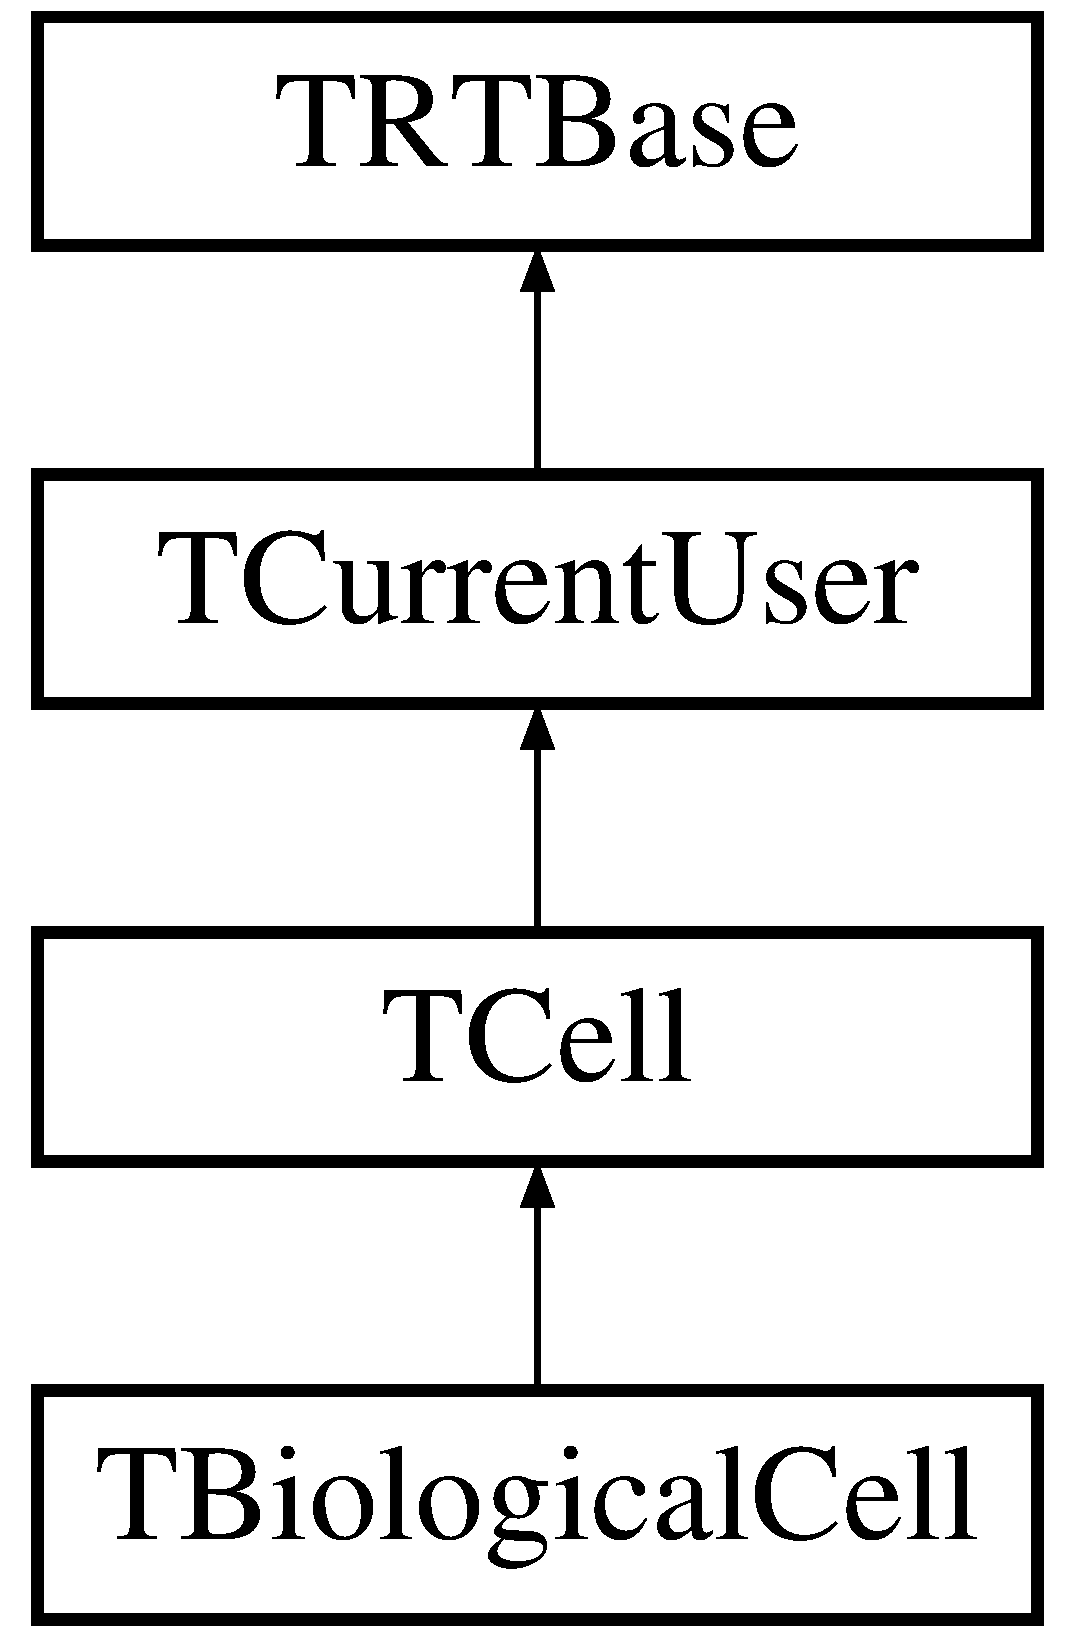
\includegraphics[height=4.000000cm]{class_t_biological_cell}
\end{center}
\end{figure}
\subsection*{Public Member Functions}
\begin{DoxyCompactItemize}
\item 
virtual void $\ast$const \+\_\+\+\_\+fastcall \hyperlink{class_t_biological_cell_a35a6350ccd6c518944f15902edc1c608}{Get\+Edit\+Form} ()
\item 
\hypertarget{class_t_biological_cell_a48bf395e0823aca37b48c5027cd525e2}{virtual void \+\_\+\+\_\+fastcall \hyperlink{class_t_biological_cell_a48bf395e0823aca37b48c5027cd525e2}{Populate\+Edit\+Form} ()}\label{class_t_biological_cell_a48bf395e0823aca37b48c5027cd525e2}

\begin{DoxyCompactList}\small\item\em Interface for derived classes, called by G\+U\+I to update V\+C\+L form components. \end{DoxyCompactList}\item 
\hypertarget{class_t_biological_cell_a5dcafb440645c90d2783e571dcdb06df}{virtual bool \+\_\+\+\_\+fastcall \hyperlink{class_t_biological_cell_a5dcafb440645c90d2783e571dcdb06df}{Validate\+Edit\+Form} ()}\label{class_t_biological_cell_a5dcafb440645c90d2783e571dcdb06df}

\begin{DoxyCompactList}\small\item\em Interface for derived classes, called by G\+U\+I to read V\+C\+L form values. \end{DoxyCompactList}\item 
\hypertarget{class_t_biological_cell_a8f09d1b52670bdff61c8beacb56ceacc}{\+\_\+\+\_\+fastcall \hyperlink{class_t_biological_cell_a8f09d1b52670bdff61c8beacb56ceacc}{T\+Biological\+Cell} ()}\label{class_t_biological_cell_a8f09d1b52670bdff61c8beacb56ceacc}

\begin{DoxyCompactList}\small\item\em Default constructor. \end{DoxyCompactList}\item 
\hypertarget{class_t_biological_cell_a53193dc5afdaa91fa5a51d5c1fefc579}{\+\_\+\+\_\+fastcall \hyperlink{class_t_biological_cell_a53193dc5afdaa91fa5a51d5c1fefc579}{T\+Biological\+Cell} (const std\+::wstring \&name)}\label{class_t_biological_cell_a53193dc5afdaa91fa5a51d5c1fefc579}

\begin{DoxyCompactList}\small\item\em Specialized constructor. \end{DoxyCompactList}\item 
\hypertarget{class_t_biological_cell_a84b78f66ee93ad556dfd08d3c6bb86ab}{\+\_\+\+\_\+fastcall \hyperlink{class_t_biological_cell_a84b78f66ee93ad556dfd08d3c6bb86ab}{T\+Biological\+Cell} (const \hyperlink{class_t_biological_cell}{T\+Biological\+Cell} \&source)}\label{class_t_biological_cell_a84b78f66ee93ad556dfd08d3c6bb86ab}

\begin{DoxyCompactList}\small\item\em Copy constructor. \end{DoxyCompactList}\item 
\hypertarget{class_t_biological_cell_a3f2c8a0990ea1c461341a9290add4cc9}{\hyperlink{class_t_biological_cell}{T\+Biological\+Cell} \& \hyperlink{class_t_biological_cell_a3f2c8a0990ea1c461341a9290add4cc9}{operator=} (const \hyperlink{class_t_biological_cell}{T\+Biological\+Cell} \&source)}\label{class_t_biological_cell_a3f2c8a0990ea1c461341a9290add4cc9}

\begin{DoxyCompactList}\small\item\em Overloaded assignment operator. \end{DoxyCompactList}\item 
\hypertarget{class_t_biological_cell_a05e8945af2d83f4a7c4d10227af62c00}{virtual double \+\_\+\+\_\+fastcall \hyperlink{class_t_biological_cell_a05e8945af2d83f4a7c4d10227af62c00}{Set\+Vm} (double \hyperlink{class_t_cell_afd81f2fd923ffbfa5ea7eda2c50693d1}{Vm})}\label{class_t_biological_cell_a05e8945af2d83f4a7c4d10227af62c00}

\begin{DoxyCompactList}\small\item\em Sets the membrane voltage. \end{DoxyCompactList}\item 
\hypertarget{class_t_biological_cell_a1d4ee3bb8f2896a4184ee41e2eb9abb4}{virtual double \+\_\+\+\_\+fastcall \hyperlink{class_t_biological_cell_a1d4ee3bb8f2896a4184ee41e2eb9abb4}{Calc\+Vm} (double step)}\label{class_t_biological_cell_a1d4ee3bb8f2896a4184ee41e2eb9abb4}

\begin{DoxyCompactList}\small\item\em overridden, but not used because cell is voltage dependent \end{DoxyCompactList}\item 
\hypertarget{class_t_biological_cell_ab862a6ed960895ffbc1b38c56955f447}{bool \+\_\+\+\_\+fastcall \hyperlink{class_t_biological_cell_ab862a6ed960895ffbc1b38c56955f447}{Is\+Voltage\+Dependent} ()}\label{class_t_biological_cell_ab862a6ed960895ffbc1b38c56955f447}

\begin{DoxyCompactList}\small\item\em Returns true, because this cell needs voltage set by \hyperlink{class_t_biological_cell_a05e8945af2d83f4a7c4d10227af62c00}{Set\+Vm()} \end{DoxyCompactList}\item 
\hypertarget{class_t_biological_cell_a01a90abdda47cd3258a28027c52b26ac}{virtual double \+\_\+\+\_\+fastcall \hyperlink{class_t_biological_cell_a01a90abdda47cd3258a28027c52b26ac}{Do\+Update} (double step)}\label{class_t_biological_cell_a01a90abdda47cd3258a28027c52b26ac}

\begin{DoxyCompactList}\small\item\em Worker function that updates the current -- overrides \hyperlink{class_t_cell_a676e15babd5f58f19577a362f01400a3}{T\+Cell\+::\+Do\+Update} to allow for current limits. \end{DoxyCompactList}\item 
\hypertarget{class_t_biological_cell_af4c430a48bebb23cafd778587c82d910}{bool \+\_\+\+\_\+fastcall \hyperlink{class_t_biological_cell_af4c430a48bebb23cafd778587c82d910}{Initialize} (bool Reset)}\label{class_t_biological_cell_af4c430a48bebb23cafd778587c82d910}

\begin{DoxyCompactList}\small\item\em pure virtual function for resetting before networking run \end{DoxyCompactList}\item 
const std\+::wstring \&\+\_\+\+\_\+fastcall \hyperlink{class_t_biological_cell_a7006d17ad9b7cdfa4b637d32a3c6b0b5}{Class\+Key} () const 
\begin{DoxyCompactList}\small\item\em Returns string used to register class with factory. \end{DoxyCompactList}\item 
\hypertarget{class_t_biological_cell_ac4f22e1821048a61f0cf8df7f1f3b971}{virtual const bool \+\_\+\+\_\+fastcall \hyperlink{class_t_biological_cell_ac4f22e1821048a61f0cf8df7f1f3b971}{Accepts\+Currents} () const }\label{class_t_biological_cell_ac4f22e1821048a61f0cf8df7f1f3b971}

\begin{DoxyCompactList}\small\item\em Informs caller whether can accept currents or not. \end{DoxyCompactList}\end{DoxyCompactItemize}
\subsection*{Friends}
\begin{DoxyCompactItemize}
\item 
\hypertarget{class_t_biological_cell_ac98d07dd8f7b70e16ccb9a01abf56b9c}{class \hyperlink{class_t_biological_cell_ac98d07dd8f7b70e16ccb9a01abf56b9c}{boost\+::serialization\+::access}}\label{class_t_biological_cell_ac98d07dd8f7b70e16ccb9a01abf56b9c}

\begin{DoxyCompactList}\small\item\em Required for serialization and saving networks to disk. \end{DoxyCompactList}\end{DoxyCompactItemize}
\subsection*{Additional Inherited Members}


\subsection{Detailed Description}
Derived class that implements \char`\"{}dynamically clamped\char`\"{} cell. 

\hyperlink{class_t_biological_cell_a05e8945af2d83f4a7c4d10227af62c00}{Set\+Vm()} called to update membrane voltage. Then all \hyperlink{class_t_cell_ab65843b9b3021e0d2e614edb4ac1a18e}{Update()} is called so that intrinsic currents, synaptic currents, and electrode currents are calculated and summed. This value is used by data acquisition classes to inject current.

\begin{DoxyAuthor}{Author}
E. Brady Trexler $<$ebtrexler (at) gothamsci.\+com$>$, 2011 -\/ 2013 
\end{DoxyAuthor}


\subsection{Member Function Documentation}
\hypertarget{class_t_biological_cell_a7006d17ad9b7cdfa4b637d32a3c6b0b5}{\index{T\+Biological\+Cell@{T\+Biological\+Cell}!Class\+Key@{Class\+Key}}
\index{Class\+Key@{Class\+Key}!T\+Biological\+Cell@{T\+Biological\+Cell}}
\subsubsection[{Class\+Key}]{\setlength{\rightskip}{0pt plus 5cm}const std\+::wstring\& \+\_\+\+\_\+fastcall T\+Biological\+Cell\+::\+Class\+Key (
\begin{DoxyParamCaption}
{}
\end{DoxyParamCaption}
) const\hspace{0.3cm}{\ttfamily [inline]}, {\ttfamily [virtual]}}}\label{class_t_biological_cell_a7006d17ad9b7cdfa4b637d32a3c6b0b5}


Returns string used to register class with factory. 

Users of class factories must also tell the class the key they used when registering the class. See factory.\+h 

Implements \hyperlink{class_t_r_t_base_a6083fd510cbcb00faa85e5934fc3c18e}{T\+R\+T\+Base}.

\hypertarget{class_t_biological_cell_a35a6350ccd6c518944f15902edc1c608}{\index{T\+Biological\+Cell@{T\+Biological\+Cell}!Get\+Edit\+Form@{Get\+Edit\+Form}}
\index{Get\+Edit\+Form@{Get\+Edit\+Form}!T\+Biological\+Cell@{T\+Biological\+Cell}}
\subsubsection[{Get\+Edit\+Form}]{\setlength{\rightskip}{0pt plus 5cm}virtual void$\ast$ const \+\_\+\+\_\+fastcall T\+Biological\+Cell\+::\+Get\+Edit\+Form (
\begin{DoxyParamCaption}
{}
\end{DoxyParamCaption}
)\hspace{0.3cm}{\ttfamily [inline]}, {\ttfamily [virtual]}}}\label{class_t_biological_cell_a35a6350ccd6c518944f15902edc1c608}
Interface for derived classes, returns pointer to G\+U\+I object for editing members. Callers must cast pointer to the correct object. 

Implements \hyperlink{class_t_r_t_base_ab83e520005e20ee71f98f3e85e1ee6d4}{T\+R\+T\+Base}.



The documentation for this class was generated from the following file\+:\begin{DoxyCompactItemize}
\item 
G\+U\+I\+\_\+\+R\+T\+\_\+\+Edit\+\_\+\+Biological\+Cell.\+cpp\end{DoxyCompactItemize}

\hypertarget{class_t_biological_cell_form}{\section{T\+Biological\+Cell\+Form Class Reference}
\label{class_t_biological_cell_form}\index{T\+Biological\+Cell\+Form@{T\+Biological\+Cell\+Form}}
}


G\+U\+I editor for \hyperlink{class_t_biological_cell}{T\+Biological\+Cell}.  




{\ttfamily \#include $<$G\+U\+I\+\_\+\+R\+T\+\_\+\+Edit\+\_\+\+Biological\+Cell.\+h$>$}

Inheritance diagram for T\+Biological\+Cell\+Form\+:\begin{figure}[H]
\begin{center}
\leavevmode
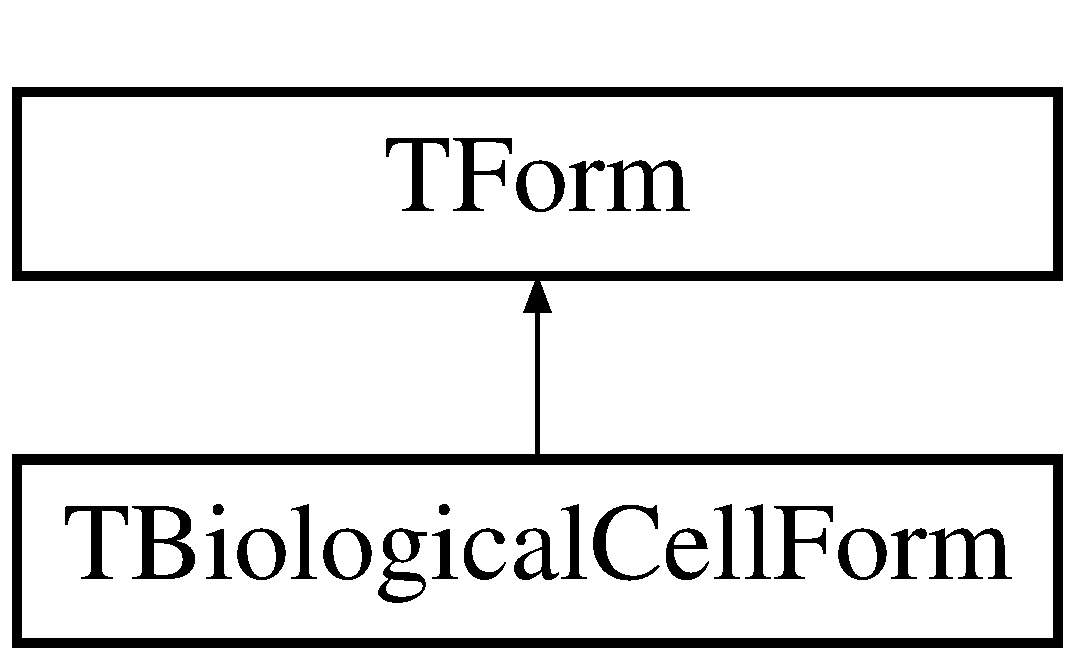
\includegraphics[height=2.000000cm]{class_t_biological_cell_form}
\end{center}
\end{figure}
\subsection*{Public Member Functions}
\begin{DoxyCompactItemize}
\item 
\hypertarget{class_t_biological_cell_form_afa19b9480377ba095705a7d98a6df242}{void \+\_\+\+\_\+fastcall {\bfseries Amp\+Gain\+Edit\+Key\+Press} (T\+Object $\ast$Sender, wchar\+\_\+t \&Key)}\label{class_t_biological_cell_form_afa19b9480377ba095705a7d98a6df242}

\item 
\hypertarget{class_t_biological_cell_form_aaf79b53ff9990460bce5ed4372ef1308}{void \+\_\+\+\_\+fastcall {\bfseries Network\+Gain\+Edit\+Key\+Press} (T\+Object $\ast$Sender, wchar\+\_\+t \&Key)}\label{class_t_biological_cell_form_aaf79b53ff9990460bce5ed4372ef1308}

\item 
\hypertarget{class_t_biological_cell_form_a6555268063a64cbab5a554f924aaee15}{void \+\_\+\+\_\+fastcall {\bfseries lbx\+A\+I\+A\+O\+Channels\+Click} (T\+Object $\ast$Sender)}\label{class_t_biological_cell_form_a6555268063a64cbab5a554f924aaee15}

\item 
\hypertarget{class_t_biological_cell_form_a0baaeb2ba369f54d62dc5d93b8c09e0c}{void \+\_\+\+\_\+fastcall {\bfseries Pos\+Neg\+Limit\+Edit\+Key\+Press} (T\+Object $\ast$Sender, wchar\+\_\+t \&Key)}\label{class_t_biological_cell_form_a0baaeb2ba369f54d62dc5d93b8c09e0c}

\item 
\hypertarget{class_t_biological_cell_form_a478835755a005cfba0a3b946c7579270}{\+\_\+\+\_\+fastcall {\bfseries T\+Biological\+Cell\+Form} (T\+Component $\ast$Owner)}\label{class_t_biological_cell_form_a478835755a005cfba0a3b946c7579270}

\end{DoxyCompactItemize}
\subsection*{Public Attributes}
\begin{DoxyCompactItemize}
\item 
\hypertarget{class_t_biological_cell_form_a4151817215aa06dbd9c65ce6e877d038}{T\+Label $\ast$ {\bfseries Label6}}\label{class_t_biological_cell_form_a4151817215aa06dbd9c65ce6e877d038}

\item 
\hypertarget{class_t_biological_cell_form_aeb84e1643f88b35b9c4d318f05d7c5d2}{T\+List\+Box $\ast$ {\bfseries lbx\+A\+I\+Channels}}\label{class_t_biological_cell_form_aeb84e1643f88b35b9c4d318f05d7c5d2}

\item 
\hypertarget{class_t_biological_cell_form_a2453775b644cd2009be052474c7b7bd9}{T\+Label $\ast$ {\bfseries Label7}}\label{class_t_biological_cell_form_a2453775b644cd2009be052474c7b7bd9}

\item 
\hypertarget{class_t_biological_cell_form_adee2f042629707931045d2d716cc0d9f}{T\+List\+Box $\ast$ {\bfseries lbx\+A\+O\+Channels}}\label{class_t_biological_cell_form_adee2f042629707931045d2d716cc0d9f}

\item 
\hypertarget{class_t_biological_cell_form_a0e68ece48e29f11b2646cb77dae19a0a}{T\+Label $\ast$ {\bfseries Label1}}\label{class_t_biological_cell_form_a0e68ece48e29f11b2646cb77dae19a0a}

\item 
\hypertarget{class_t_biological_cell_form_ab050952fd68857b49501c4ffb175e6b3}{T\+Label $\ast$ {\bfseries Label2}}\label{class_t_biological_cell_form_ab050952fd68857b49501c4ffb175e6b3}

\item 
\hypertarget{class_t_biological_cell_form_a3f8acbaa94296c682261d8c416f4a749}{T\+Label $\ast$ {\bfseries Label3}}\label{class_t_biological_cell_form_a3f8acbaa94296c682261d8c416f4a749}

\item 
\hypertarget{class_t_biological_cell_form_a316960037945a79be67a25739c51af1b}{T\+Label $\ast$ {\bfseries Label4}}\label{class_t_biological_cell_form_a316960037945a79be67a25739c51af1b}

\item 
\hypertarget{class_t_biological_cell_form_a56040dabf7b19f32450040d1fe735202}{T\+Edit $\ast$ {\bfseries A\+I\+Gain\+Edit}}\label{class_t_biological_cell_form_a56040dabf7b19f32450040d1fe735202}

\item 
\hypertarget{class_t_biological_cell_form_aa951699926b4d124e80e506b39f796ea}{T\+Edit $\ast$ {\bfseries A\+O\+Gain\+Edit}}\label{class_t_biological_cell_form_aa951699926b4d124e80e506b39f796ea}

\item 
\hypertarget{class_t_biological_cell_form_ad91293468d6062ae4ae8ef1103ec4d0e}{T\+Label $\ast$ {\bfseries Label5}}\label{class_t_biological_cell_form_ad91293468d6062ae4ae8ef1103ec4d0e}

\item 
\hypertarget{class_t_biological_cell_form_af6f581c85f7330d622dc02a2c1f5cb57}{T\+Edit $\ast$ {\bfseries A\+D\+C\+Gain\+Edit}}\label{class_t_biological_cell_form_af6f581c85f7330d622dc02a2c1f5cb57}

\item 
\hypertarget{class_t_biological_cell_form_ae9f04c6b09cd1efc1a499d918877f24e}{T\+Label $\ast$ {\bfseries Label8}}\label{class_t_biological_cell_form_ae9f04c6b09cd1efc1a499d918877f24e}

\item 
\hypertarget{class_t_biological_cell_form_a58a9e6d96198fcddd8c6cd0b42949273}{T\+Edit $\ast$ {\bfseries D\+A\+C\+Gain\+Edit}}\label{class_t_biological_cell_form_a58a9e6d96198fcddd8c6cd0b42949273}

\item 
\hypertarget{class_t_biological_cell_form_a7b2e9ba55dea0289d3895373bab5289a}{T\+Label $\ast$ {\bfseries Label9}}\label{class_t_biological_cell_form_a7b2e9ba55dea0289d3895373bab5289a}

\item 
\hypertarget{class_t_biological_cell_form_aaa4a21719e62c7d65d5f957b69f71122}{T\+Panel $\ast$ {\bfseries Panel1}}\label{class_t_biological_cell_form_aaa4a21719e62c7d65d5f957b69f71122}

\item 
\hypertarget{class_t_biological_cell_form_a58526eddac62e22db84f761b5ace7e03}{T\+Panel $\ast$ {\bfseries Panel2}}\label{class_t_biological_cell_form_a58526eddac62e22db84f761b5ace7e03}

\item 
\hypertarget{class_t_biological_cell_form_a63fa28ca9aee45465cf62056316b2d1a}{T\+Label $\ast$ {\bfseries Label10}}\label{class_t_biological_cell_form_a63fa28ca9aee45465cf62056316b2d1a}

\item 
\hypertarget{class_t_biological_cell_form_a8c4cc8fc2eefad18c90b9d2615e48165}{T\+Label $\ast$ {\bfseries Label11}}\label{class_t_biological_cell_form_a8c4cc8fc2eefad18c90b9d2615e48165}

\item 
\hypertarget{class_t_biological_cell_form_a4ae380569b7b7885ac5260e613ec3452}{T\+Label $\ast$ {\bfseries Label12}}\label{class_t_biological_cell_form_a4ae380569b7b7885ac5260e613ec3452}

\item 
\hypertarget{class_t_biological_cell_form_adba374de4b673ac141ceea5ac563adc0}{T\+Edit $\ast$ {\bfseries Pos\+Limit\+Edit}}\label{class_t_biological_cell_form_adba374de4b673ac141ceea5ac563adc0}

\item 
\hypertarget{class_t_biological_cell_form_a6643cacc641ee2b4de0c6c5a7b7e9a0b}{T\+Edit $\ast$ {\bfseries Neg\+Limit\+Edit}}\label{class_t_biological_cell_form_a6643cacc641ee2b4de0c6c5a7b7e9a0b}

\item 
\hypertarget{class_t_biological_cell_form_a2e255332b76a7e91fa2a61577d29d19d}{T\+Label $\ast$ {\bfseries Label13}}\label{class_t_biological_cell_form_a2e255332b76a7e91fa2a61577d29d19d}

\item 
\hypertarget{class_t_biological_cell_form_ac17b732fdc51516bf96f960eea1eed0e}{T\+Label $\ast$ {\bfseries Label14}}\label{class_t_biological_cell_form_ac17b732fdc51516bf96f960eea1eed0e}

\item 
\hypertarget{class_t_biological_cell_form_a2ef94b84caa3e94b597ecccac07f6e7b}{\hyperlink{class_t_biological_cell}{T\+Biological\+Cell} $\ast$ {\bfseries Biological\+Cell}}\label{class_t_biological_cell_form_a2ef94b84caa3e94b597ecccac07f6e7b}

\end{DoxyCompactItemize}


\subsection{Detailed Description}
G\+U\+I editor for \hyperlink{class_t_biological_cell}{T\+Biological\+Cell}. 

\begin{DoxyAuthor}{Author}
E. Brady Trexler $<$ebtrexler (at) gothamsci.\+com$>$, 2011 -\/ 2013 
\end{DoxyAuthor}


The documentation for this class was generated from the following files\+:\begin{DoxyCompactItemize}
\item 
G\+U\+I\+\_\+\+R\+T\+\_\+\+Edit\+\_\+\+Biological\+Cell.\+h\item 
G\+U\+I\+\_\+\+R\+T\+\_\+\+Edit\+\_\+\+Biological\+Cell.\+cpp\end{DoxyCompactItemize}

\hypertarget{class_t_cell}{\section{T\+Cell Class Reference}
\label{class_t_cell}\index{T\+Cell@{T\+Cell}}
}


Base class for biological and model and other specialized cells.  




{\ttfamily \#include $<$R\+T\+\_\+\+Cell.\+h$>$}

Inheritance diagram for T\+Cell\+:\begin{figure}[H]
\begin{center}
\leavevmode
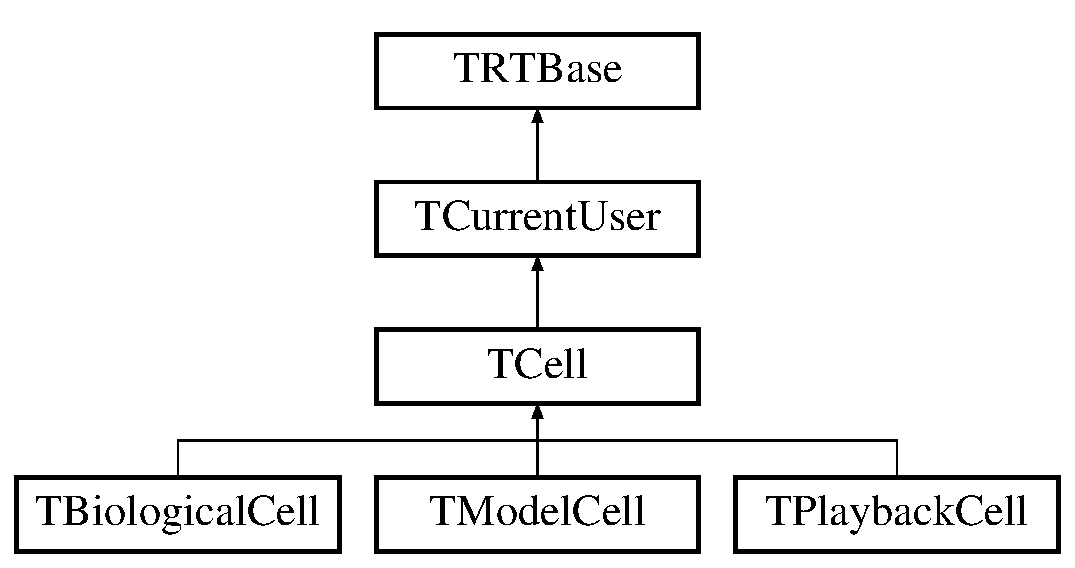
\includegraphics[height=4.000000cm]{class_t_cell}
\end{center}
\end{figure}
\subsection*{Public Member Functions}
\begin{DoxyCompactItemize}
\item 
\hypertarget{class_t_cell_a21058e4555fbca0016550e81acfe85b7}{virtual std\+::wstring \+\_\+\+\_\+fastcall \hyperlink{class_t_cell_a21058e4555fbca0016550e81acfe85b7}{A\+I\+Channel} ()}\label{class_t_cell_a21058e4555fbca0016550e81acfe85b7}

\begin{DoxyCompactList}\small\item\em Returns the Analog Input Channel for this cell, if assigned. \end{DoxyCompactList}\item 
\hypertarget{class_t_cell_aff448a0cbbe96e528d59518b9cd20075}{virtual std\+::wstring \+\_\+\+\_\+fastcall \hyperlink{class_t_cell_aff448a0cbbe96e528d59518b9cd20075}{A\+O\+Channel} ()}\label{class_t_cell_aff448a0cbbe96e528d59518b9cd20075}

\begin{DoxyCompactList}\small\item\em Returns the Analog Output Channel for this cell, if assigned. \end{DoxyCompactList}\item 
\hypertarget{class_t_cell_a3a3f8f9d1da6b19cbb0e7faa9d8fe36b}{virtual double \+\_\+\+\_\+fastcall \hyperlink{class_t_cell_a3a3f8f9d1da6b19cbb0e7faa9d8fe36b}{A\+I\+Gain} ()}\label{class_t_cell_a3a3f8f9d1da6b19cbb0e7faa9d8fe36b}

\begin{DoxyCompactList}\small\item\em Returns the Analog Input Gain for this cell, if assigned. \end{DoxyCompactList}\item 
\hypertarget{class_t_cell_acacc3c2214db5f5593ad87d3255c0946}{virtual double \+\_\+\+\_\+fastcall \hyperlink{class_t_cell_acacc3c2214db5f5593ad87d3255c0946}{A\+O\+Gain} ()}\label{class_t_cell_acacc3c2214db5f5593ad87d3255c0946}

\begin{DoxyCompactList}\small\item\em Returns the Analog Output Gain for this cell, if assigned. \end{DoxyCompactList}\item 
\hypertarget{class_t_cell_a98c54f012c9f9b55294d3f055af7be33}{virtual double \+\_\+\+\_\+fastcall \hyperlink{class_t_cell_a98c54f012c9f9b55294d3f055af7be33}{I} ()}\label{class_t_cell_a98c54f012c9f9b55294d3f055af7be33}

\begin{DoxyCompactList}\small\item\em Returns the current value of the calculated current. \end{DoxyCompactList}\item 
\hypertarget{class_t_cell_afd81f2fd923ffbfa5ea7eda2c50693d1}{virtual double \+\_\+\+\_\+fastcall \hyperlink{class_t_cell_afd81f2fd923ffbfa5ea7eda2c50693d1}{Vm} ()}\label{class_t_cell_afd81f2fd923ffbfa5ea7eda2c50693d1}

\begin{DoxyCompactList}\small\item\em Returns the stored value of the membrane potential. \end{DoxyCompactList}\item 
\hypertarget{class_t_cell_a8b7f6098ca372dac0b4b45c361bcaa64}{virtual double \+\_\+\+\_\+fastcall \hyperlink{class_t_cell_a8b7f6098ca372dac0b4b45c361bcaa64}{Set\+Vm} (double \hyperlink{class_t_cell_afd81f2fd923ffbfa5ea7eda2c50693d1}{Vm})=0}\label{class_t_cell_a8b7f6098ca372dac0b4b45c361bcaa64}

\begin{DoxyCompactList}\small\item\em Sets membrane voltage -- must be overriden. \end{DoxyCompactList}\item 
\hypertarget{class_t_cell_a052db3a15a6d2c93b475fc71198c46c7}{virtual double \+\_\+\+\_\+fastcall \hyperlink{class_t_cell_a052db3a15a6d2c93b475fc71198c46c7}{Calc\+Vm} (double step)=0}\label{class_t_cell_a052db3a15a6d2c93b475fc71198c46c7}

\begin{DoxyCompactList}\small\item\em Calculates membrane voltage -- must be overridden. \end{DoxyCompactList}\item 
\hypertarget{class_t_cell_abbdbd5f05d4ae7ec2a311444416072de}{virtual bool \+\_\+\+\_\+fastcall \hyperlink{class_t_cell_abbdbd5f05d4ae7ec2a311444416072de}{Is\+Voltage\+Dependent} ()=0}\label{class_t_cell_abbdbd5f05d4ae7ec2a311444416072de}

\begin{DoxyCompactList}\small\item\em Used to classify cell as biological (true) or other (false) \end{DoxyCompactList}\item 
\hypertarget{class_t_cell_a676e15babd5f58f19577a362f01400a3}{virtual double \+\_\+\+\_\+fastcall \hyperlink{class_t_cell_a676e15babd5f58f19577a362f01400a3}{Do\+Update} (double step)}\label{class_t_cell_a676e15babd5f58f19577a362f01400a3}

\begin{DoxyCompactList}\small\item\em Worker function that updates the current -- no need to override. \end{DoxyCompactList}\item 
double \+\_\+\+\_\+fastcall \hyperlink{class_t_cell_ab65843b9b3021e0d2e614edb4ac1a18e}{Update} (double step)
\begin{DoxyCompactList}\small\item\em Checks if Active, and if so, calls Do\+Update to calculate the new current. \end{DoxyCompactList}\item 
\hypertarget{class_t_cell_ad3dc989fecc587656dfc2f8570dfe772}{virtual const \hyperlink{class_t_current}{T\+Current} $\ast$\+\_\+\+\_\+fastcall \hyperlink{class_t_cell_ad3dc989fecc587656dfc2f8570dfe772}{Add\+Current} (\hyperlink{class_t_current}{T\+Current} $\ast$const c, \hyperlink{class_t_cell}{T\+Cell} $\ast$cell=N\+U\+L\+L)}\label{class_t_cell_ad3dc989fecc587656dfc2f8570dfe772}

\begin{DoxyCompactList}\small\item\em Adds a \hyperlink{class_t_current}{T\+Current} $\ast$ to the array of Currents. \end{DoxyCompactList}\item 
\hypertarget{class_t_cell_af0d4c09293bffc70c99f12de3500edc4}{virtual void \+\_\+\+\_\+fastcall \hyperlink{class_t_cell_af0d4c09293bffc70c99f12de3500edc4}{Remove\+Current} (\hyperlink{class_t_current}{T\+Current} $\ast$c)}\label{class_t_cell_af0d4c09293bffc70c99f12de3500edc4}

\begin{DoxyCompactList}\small\item\em Removes a \hyperlink{class_t_current}{T\+Current} $\ast$ from the array of Currents. \end{DoxyCompactList}\item 
\hypertarget{class_t_cell_a010e6020a66c58784a97c7acbbf51c96}{virtual const T\+Currents\+Array \\*
\+\_\+\+\_\+fastcall \hyperlink{class_t_cell_a010e6020a66c58784a97c7acbbf51c96}{Get\+Currents} () const }\label{class_t_cell_a010e6020a66c58784a97c7acbbf51c96}

\begin{DoxyCompactList}\small\item\em Returns the array of Currents. \end{DoxyCompactList}\item 
\hypertarget{class_t_cell_a64b8f989fa47f0ee79942f5b9d2cafa8}{void \+\_\+\+\_\+fastcall \hyperlink{class_t_cell_a64b8f989fa47f0ee79942f5b9d2cafa8}{Clear\+Currents} ()}\label{class_t_cell_a64b8f989fa47f0ee79942f5b9d2cafa8}

\begin{DoxyCompactList}\small\item\em Deletes all currents from the cell. \end{DoxyCompactList}\item 
\hypertarget{class_t_cell_a4d5ecf99d9b4ec0f08d43eac2cbe1b54}{virtual const bool \+\_\+\+\_\+fastcall \hyperlink{class_t_cell_a4d5ecf99d9b4ec0f08d43eac2cbe1b54}{Accepts\+Currents} () const =0}\label{class_t_cell_a4d5ecf99d9b4ec0f08d43eac2cbe1b54}

\begin{DoxyCompactList}\small\item\em Informs caller whether can accept currents or not. \end{DoxyCompactList}\item 
\hypertarget{class_t_cell_a9b2c6a2758b286d456a46dbf917e6c72}{virtual const \hyperlink{class_t_synapse}{T\+Synapse} $\ast$\+\_\+\+\_\+fastcall \hyperlink{class_t_cell_a9b2c6a2758b286d456a46dbf917e6c72}{Add\+Synapse} (\hyperlink{class_t_synapse}{T\+Synapse} $\ast$s)}\label{class_t_cell_a9b2c6a2758b286d456a46dbf917e6c72}

\begin{DoxyCompactList}\small\item\em Adds a \hyperlink{class_t_synapse}{T\+Synapse} $\ast$ to the array of Synapses. \end{DoxyCompactList}\item 
\hypertarget{class_t_cell_aec972dfd296c80ab77b8bfcfab5746dd}{virtual void \+\_\+\+\_\+fastcall \hyperlink{class_t_cell_aec972dfd296c80ab77b8bfcfab5746dd}{Remove\+Synapse} (\hyperlink{class_t_synapse}{T\+Synapse} $\ast$s)}\label{class_t_cell_aec972dfd296c80ab77b8bfcfab5746dd}

\begin{DoxyCompactList}\small\item\em Removes a \hyperlink{class_t_synapse}{T\+Synapse} $\ast$ from the array of Synapses. \end{DoxyCompactList}\item 
\hypertarget{class_t_cell_a1382dc952b5116fa6dfd12b9b184c734}{virtual const T\+Synapses\+Array \\*
\+\_\+\+\_\+fastcall \hyperlink{class_t_cell_a1382dc952b5116fa6dfd12b9b184c734}{Get\+Synapses} () const }\label{class_t_cell_a1382dc952b5116fa6dfd12b9b184c734}

\begin{DoxyCompactList}\small\item\em Returns the array of Synapses. \end{DoxyCompactList}\item 
\hypertarget{class_t_cell_ab80546f10ffdac768ec2ec51924fda32}{virtual const \hyperlink{class_t_electrode}{T\+Electrode} \\*
$\ast$\+\_\+\+\_\+fastcall \hyperlink{class_t_cell_ab80546f10ffdac768ec2ec51924fda32}{Add\+Electrode} (\hyperlink{class_t_electrode}{T\+Electrode} $\ast$e)}\label{class_t_cell_ab80546f10ffdac768ec2ec51924fda32}

\begin{DoxyCompactList}\small\item\em Adds a \hyperlink{class_t_electrode}{T\+Electrode} $\ast$ to the array of Electrodes. \end{DoxyCompactList}\item 
\hypertarget{class_t_cell_a75dcebc4e5e9e6363193931c286b61bf}{virtual void \+\_\+\+\_\+fastcall \hyperlink{class_t_cell_a75dcebc4e5e9e6363193931c286b61bf}{Remove\+Electrode} (\hyperlink{class_t_electrode}{T\+Electrode} $\ast$e)}\label{class_t_cell_a75dcebc4e5e9e6363193931c286b61bf}

\begin{DoxyCompactList}\small\item\em Removes a \hyperlink{class_t_electrode}{T\+Electrode} $\ast$ from the array of Electrodes. \end{DoxyCompactList}\item 
\hypertarget{class_t_cell_a87793cac2e21de67e5892363418f84f3}{virtual const T\+Electrodes\+Array \\*
\+\_\+\+\_\+fastcall \hyperlink{class_t_cell_a87793cac2e21de67e5892363418f84f3}{Get\+Electrodes} () const }\label{class_t_cell_a87793cac2e21de67e5892363418f84f3}

\begin{DoxyCompactList}\small\item\em Returns the array of Electrodes. \end{DoxyCompactList}\item 
\hypertarget{class_t_cell_a0d30cc0ed0f9f6e558011e5ee5b6abfd}{\+\_\+\+\_\+fastcall \hyperlink{class_t_cell_a0d30cc0ed0f9f6e558011e5ee5b6abfd}{T\+Cell} ()}\label{class_t_cell_a0d30cc0ed0f9f6e558011e5ee5b6abfd}

\begin{DoxyCompactList}\small\item\em Default constructor. \end{DoxyCompactList}\item 
\hypertarget{class_t_cell_ad5dd987fa88c278edf15aad34ffef153}{\+\_\+\+\_\+fastcall \hyperlink{class_t_cell_ad5dd987fa88c278edf15aad34ffef153}{T\+Cell} (const std\+::wstring \&name)}\label{class_t_cell_ad5dd987fa88c278edf15aad34ffef153}

\begin{DoxyCompactList}\small\item\em Specialized constructor. \end{DoxyCompactList}\item 
\hypertarget{class_t_cell_a1a02301a30115d7c52b5fdbb0e6fedf0}{\+\_\+\+\_\+fastcall \hyperlink{class_t_cell_a1a02301a30115d7c52b5fdbb0e6fedf0}{T\+Cell} (const \hyperlink{class_t_cell}{T\+Cell} \&source)}\label{class_t_cell_a1a02301a30115d7c52b5fdbb0e6fedf0}

\begin{DoxyCompactList}\small\item\em Copy constructor. \end{DoxyCompactList}\item 
\hypertarget{class_t_cell_a440399879aa0643cf8d72b5137c6937f}{\hyperlink{class_t_cell}{T\+Cell} \& \hyperlink{class_t_cell_a440399879aa0643cf8d72b5137c6937f}{operator=} (const \hyperlink{class_t_cell}{T\+Cell} \&source)}\label{class_t_cell_a440399879aa0643cf8d72b5137c6937f}

\begin{DoxyCompactList}\small\item\em Overloaded assignment operator. \end{DoxyCompactList}\end{DoxyCompactItemize}
\subsection*{Protected Member Functions}
\begin{DoxyCompactItemize}
\item 
\hypertarget{class_t_cell_a30a737eed36e2927d8889f913e3a4c3a}{virtual void const \+\_\+\+\_\+fastcall \hyperlink{class_t_cell_a30a737eed36e2927d8889f913e3a4c3a}{Write\+To\+Stream} (ostream \&stream) const }\label{class_t_cell_a30a737eed36e2927d8889f913e3a4c3a}

\begin{DoxyCompactList}\small\item\em Writes data members to a stream. \end{DoxyCompactList}\item 
\hypertarget{class_t_cell_a9d7aacc69150c73ce6f3a0773cb2ae2e}{void const \+\_\+\+\_\+fastcall \hyperlink{class_t_cell_a9d7aacc69150c73ce6f3a0773cb2ae2e}{Read\+From\+Stream} (istream \&stream)}\label{class_t_cell_a9d7aacc69150c73ce6f3a0773cb2ae2e}

\begin{DoxyCompactList}\small\item\em Reads data members from a stream. \end{DoxyCompactList}\end{DoxyCompactItemize}
\subsection*{Protected Attributes}
\begin{DoxyCompactItemize}
\item 
\hypertarget{class_t_cell_a602de7c2375475244dbde16fc32863db}{std\+::wstring {\bfseries F\+A\+I\+Channel}}\label{class_t_cell_a602de7c2375475244dbde16fc32863db}

\item 
\hypertarget{class_t_cell_a538983b268916cbed077d82b8a2d478c}{std\+::wstring {\bfseries F\+A\+O\+Channel}}\label{class_t_cell_a538983b268916cbed077d82b8a2d478c}

\item 
\hypertarget{class_t_cell_aef8b4ac3536dcb9a0b100452500d5a6a}{double {\bfseries F\+A\+I\+Gain}}\label{class_t_cell_aef8b4ac3536dcb9a0b100452500d5a6a}

\item 
\hypertarget{class_t_cell_a7794f29d89012e170e50fbe116d7afd1}{double {\bfseries F\+A\+O\+Gain}}\label{class_t_cell_a7794f29d89012e170e50fbe116d7afd1}

\item 
\hypertarget{class_t_cell_ac83e5843dfdaff29d20bd6fe3c1c1b22}{double {\bfseries F\+\_\+\+Vm}}\label{class_t_cell_ac83e5843dfdaff29d20bd6fe3c1c1b22}

\item 
\hypertarget{class_t_cell_a16116f4581383ebf84d3d8d0650afe60}{double {\bfseries F\+\_\+\+I}}\label{class_t_cell_a16116f4581383ebf84d3d8d0650afe60}

\end{DoxyCompactItemize}
\subsection*{Friends}
\begin{DoxyCompactItemize}
\item 
\hypertarget{class_t_cell_ac98d07dd8f7b70e16ccb9a01abf56b9c}{class \hyperlink{class_t_cell_ac98d07dd8f7b70e16ccb9a01abf56b9c}{boost\+::serialization\+::access}}\label{class_t_cell_ac98d07dd8f7b70e16ccb9a01abf56b9c}

\begin{DoxyCompactList}\small\item\em Required for serialization and saving networks to disk. \end{DoxyCompactList}\end{DoxyCompactItemize}


\subsection{Detailed Description}
Base class for biological and model and other specialized cells. 

\hyperlink{class_t_cell}{T\+Cell} owns one array each of Currents, Electrodes, and Synapses. \hyperlink{class_t_cell}{T\+Cell}'s \hyperlink{class_t_cell_a676e15babd5f58f19577a362f01400a3}{Do\+Update(double step)} member function calls the Update functions of its Currents, Electrodes, and Synapses in a loop, summing each contribution to calculate the total current and storing the value. \hyperlink{class_t_cell}{T\+Cell} has a virtual member function--$>$ bool \hyperlink{class_t_cell_a052db3a15a6d2c93b475fc71198c46c7}{Calc\+Vm()} that will allow derived cells such as \hyperlink{class_t_model_cell}{T\+Model\+Cell} and \hyperlink{class_t_playback_cell}{T\+Playback\+Cell} to update F\+\_\+\+Vm independently of data acquisition. In addition, \hyperlink{class_t_cell_a052db3a15a6d2c93b475fc71198c46c7}{Calc\+Vm()} can be used to compare against the sampled Vm from biological cells to find a best fit for the membrane capacitance of model cells.

\begin{DoxyAuthor}{Author}
E. Brady Trexler $<$ebtrexler (at) gothamsci.\+com$>$, 2011 -\/ 2013 
\end{DoxyAuthor}


\subsection{Member Function Documentation}
\hypertarget{class_t_cell_ab65843b9b3021e0d2e614edb4ac1a18e}{\index{T\+Cell@{T\+Cell}!Update@{Update}}
\index{Update@{Update}!T\+Cell@{T\+Cell}}
\subsubsection[{Update}]{\setlength{\rightskip}{0pt plus 5cm}double \+\_\+\+\_\+fastcall T\+Cell\+::\+Update (
\begin{DoxyParamCaption}
\item[{double}]{step}
\end{DoxyParamCaption}
)}}\label{class_t_cell_ab65843b9b3021e0d2e614edb4ac1a18e}


Checks if Active, and if so, calls Do\+Update to calculate the new current. 

Before calling Update, caller must \hyperlink{class_t_cell_a8b7f6098ca372dac0b4b45c361bcaa64}{Set\+Vm()} or \hyperlink{class_t_cell_a052db3a15a6d2c93b475fc71198c46c7}{Calc\+Vm()}. 

The documentation for this class was generated from the following files\+:\begin{DoxyCompactItemize}
\item 
R\+T\+\_\+\+Cell.\+h\item 
R\+T\+\_\+\+Cell.\+cpp\end{DoxyCompactItemize}

\hypertarget{struct_t_cell_position}{\section{T\+Cell\+Position Struct Reference}
\label{struct_t_cell_position}\index{T\+Cell\+Position@{T\+Cell\+Position}}
}


Class to facilitate drawing of networks as cells arranged evenly around a circle.  




{\ttfamily \#include $<$G\+U\+I\+\_\+\+Circle\+Perimeter\+Editor.\+h$>$}

\subsection*{Public Attributes}
\begin{DoxyCompactItemize}
\item 
\hypertarget{struct_t_cell_position_a9403569f9d252768c68f14e11fa866d8}{double {\bfseries X}}\label{struct_t_cell_position_a9403569f9d252768c68f14e11fa866d8}

\item 
\hypertarget{struct_t_cell_position_a7f80d7def2e0467a29dbaf827185d7da}{double {\bfseries Y}}\label{struct_t_cell_position_a7f80d7def2e0467a29dbaf827185d7da}

\item 
\hypertarget{struct_t_cell_position_a69fcd1a26b436ca9b904d99cac217035}{double {\bfseries angle}}\label{struct_t_cell_position_a69fcd1a26b436ca9b904d99cac217035}

\end{DoxyCompactItemize}


\subsection{Detailed Description}
Class to facilitate drawing of networks as cells arranged evenly around a circle. 

\begin{DoxyAuthor}{Author}
E. Brady Trexler $<$ebtrexler (at) gothamsci.\+com$>$, 2011 -\/ 2013 
\end{DoxyAuthor}


The documentation for this struct was generated from the following file\+:\begin{DoxyCompactItemize}
\item 
G\+U\+I\+\_\+\+Circle\+Perimeter\+Editor.\+h\end{DoxyCompactItemize}

\hypertarget{class_t_copy_currents_form}{\section{T\+Copy\+Currents\+Form Class Reference}
\label{class_t_copy_currents_form}\index{T\+Copy\+Currents\+Form@{T\+Copy\+Currents\+Form}}
}


G\+U\+I class for copying currents from one cell to one or many others.  




{\ttfamily \#include $<$G\+U\+I\+\_\+\+Copy\+Currents\+Form.\+h$>$}

Inheritance diagram for T\+Copy\+Currents\+Form\+:\begin{figure}[H]
\begin{center}
\leavevmode
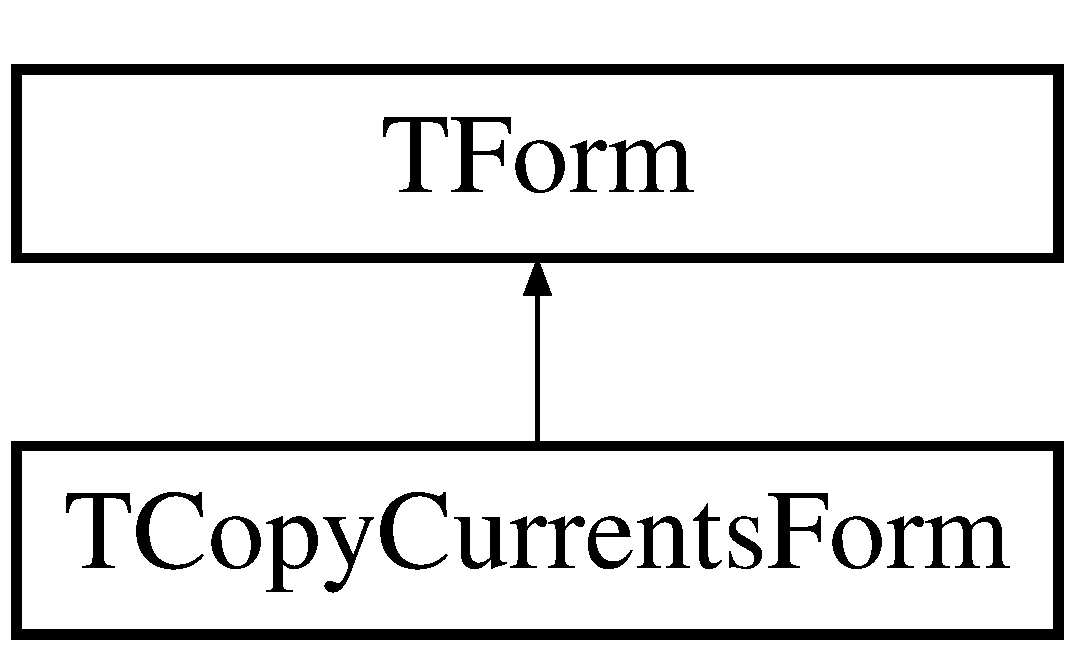
\includegraphics[height=2.000000cm]{class_t_copy_currents_form}
\end{center}
\end{figure}
\subsection*{Public Member Functions}
\begin{DoxyCompactItemize}
\item 
\hypertarget{class_t_copy_currents_form_a1149e37ecf8669f6988ce052ee9b37ea}{\+\_\+\+\_\+fastcall {\bfseries T\+Copy\+Currents\+Form} (T\+Component $\ast$Owner)}\label{class_t_copy_currents_form_a1149e37ecf8669f6988ce052ee9b37ea}

\end{DoxyCompactItemize}
\subsection*{Public Attributes}
\begin{DoxyCompactItemize}
\item 
\hypertarget{class_t_copy_currents_form_ada9a1f5ae852e881ac216a13282fbb74}{T\+Combo\+Box $\ast$ {\bfseries Copy\+From\+Combo\+Box}}\label{class_t_copy_currents_form_ada9a1f5ae852e881ac216a13282fbb74}

\item 
\hypertarget{class_t_copy_currents_form_ad601405abe7f41fe9bccc4e8a605bde5}{T\+List\+Box $\ast$ {\bfseries Copy\+To\+List\+Box}}\label{class_t_copy_currents_form_ad601405abe7f41fe9bccc4e8a605bde5}

\item 
\hypertarget{class_t_copy_currents_form_acd3c1305a949333e82e9fbdd7adc3794}{T\+Label $\ast$ {\bfseries Label1}}\label{class_t_copy_currents_form_acd3c1305a949333e82e9fbdd7adc3794}

\item 
\hypertarget{class_t_copy_currents_form_afa580bb34184774832d65916cab53614}{T\+Label $\ast$ {\bfseries Label2}}\label{class_t_copy_currents_form_afa580bb34184774832d65916cab53614}

\item 
\hypertarget{class_t_copy_currents_form_aec09380d417659ddb88da495d7d9ee1b}{T\+Button $\ast$ {\bfseries Button1}}\label{class_t_copy_currents_form_aec09380d417659ddb88da495d7d9ee1b}

\item 
\hypertarget{class_t_copy_currents_form_a898b4d631ac5b2377b22e06af1748f30}{T\+Button $\ast$ {\bfseries Button2}}\label{class_t_copy_currents_form_a898b4d631ac5b2377b22e06af1748f30}

\item 
\hypertarget{class_t_copy_currents_form_a38a1815841bf4b1d5d6e52ba1192b35e}{T\+List\+Box $\ast$ {\bfseries To\+Names\+List\+Box}}\label{class_t_copy_currents_form_a38a1815841bf4b1d5d6e52ba1192b35e}

\item 
\hypertarget{class_t_copy_currents_form_a3e18c2da6973bf19e53868eb2141d46e}{T\+Check\+Box $\ast$ {\bfseries Clear\+Then\+Copy\+Check\+Box}}\label{class_t_copy_currents_form_a3e18c2da6973bf19e53868eb2141d46e}

\end{DoxyCompactItemize}


\subsection{Detailed Description}
G\+U\+I class for copying currents from one cell to one or many others. 

\begin{DoxyAuthor}{Author}
E. Brady Trexler $<$ebtrexler (at) gothamsci.\+com$>$, 2011 -\/ 2013 
\end{DoxyAuthor}


The documentation for this class was generated from the following files\+:\begin{DoxyCompactItemize}
\item 
G\+U\+I\+\_\+\+Copy\+Currents\+Form.\+h\item 
G\+U\+I\+\_\+\+Copy\+Currents\+Form.\+cpp\end{DoxyCompactItemize}

\hypertarget{class_t_current}{\section{T\+Current Class Reference}
\label{class_t_current}\index{T\+Current@{T\+Current}}
}


Base class for all intrinsic and synaptic currents.  




{\ttfamily \#include $<$R\+T\+\_\+\+Current.\+h$>$}

Inheritance diagram for T\+Current\+:\begin{figure}[H]
\begin{center}
\leavevmode
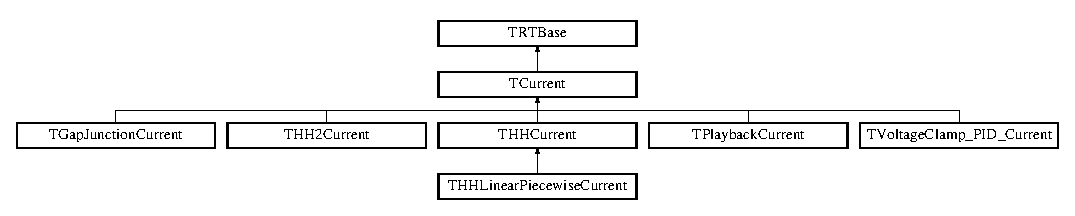
\includegraphics[height=2.461539cm]{class_t_current}
\end{center}
\end{figure}
\subsection*{Public Member Functions}
\begin{DoxyCompactItemize}
\item 
\hypertarget{class_t_current_adca3b88eb3a366b9beb2c7e1bc128b5e}{const bool \+\_\+\+\_\+fastcall \hyperlink{class_t_current_adca3b88eb3a366b9beb2c7e1bc128b5e}{Is\+Periodic} () const }\label{class_t_current_adca3b88eb3a366b9beb2c7e1bc128b5e}

\begin{DoxyCompactList}\small\item\em Gets if current is modulated according to set periodicity params. \end{DoxyCompactList}\item 
\hypertarget{class_t_current_ac7bd1741a0d5048d7e4cd3bae0a15c59}{void \+\_\+\+\_\+fastcall \hyperlink{class_t_current_ac7bd1741a0d5048d7e4cd3bae0a15c59}{Set\+Periodic} (bool isperiodic)}\label{class_t_current_ac7bd1741a0d5048d7e4cd3bae0a15c59}

\begin{DoxyCompactList}\small\item\em Sets if current is modulated according to set periodicity params. \end{DoxyCompactList}\item 
\hypertarget{class_t_current_ad5c709fa160f92c4e277d762861041df}{const double \+\_\+\+\_\+fastcall \hyperlink{class_t_current_ad5c709fa160f92c4e277d762861041df}{Get\+Period} () const }\label{class_t_current_ad5c709fa160f92c4e277d762861041df}

\begin{DoxyCompactList}\small\item\em Gets the period in ms. \end{DoxyCompactList}\item 
\hypertarget{class_t_current_a2945ddc6bc5adf79ce91f89d65d35c6f}{void \+\_\+\+\_\+fastcall \hyperlink{class_t_current_a2945ddc6bc5adf79ce91f89d65d35c6f}{Set\+Period} (double period)}\label{class_t_current_a2945ddc6bc5adf79ce91f89d65d35c6f}

\begin{DoxyCompactList}\small\item\em Sets the period in ms. \end{DoxyCompactList}\item 
\hypertarget{class_t_current_a43746954efbc4bd1c72002aafe2bb07e}{const int \+\_\+\+\_\+fastcall \hyperlink{class_t_current_a43746954efbc4bd1c72002aafe2bb07e}{Get\+Wave\+Type} () const }\label{class_t_current_a43746954efbc4bd1c72002aafe2bb07e}

\begin{DoxyCompactList}\small\item\em Gets the period type -- square or sine. \end{DoxyCompactList}\item 
\hypertarget{class_t_current_a5647d6bf68c5d83957fa1c4201ae0c7f}{void \+\_\+\+\_\+fastcall \hyperlink{class_t_current_a5647d6bf68c5d83957fa1c4201ae0c7f}{Set\+Wave\+Type} (int wavetype)}\label{class_t_current_a5647d6bf68c5d83957fa1c4201ae0c7f}

\begin{DoxyCompactList}\small\item\em Sets the period type -- square or sine. \end{DoxyCompactList}\item 
\hypertarget{class_t_current_a252da7976039d425984a0acae22e8ffe}{const double \+\_\+\+\_\+fastcall \hyperlink{class_t_current_a252da7976039d425984a0acae22e8ffe}{Get\+Duty\+Cycle} () const }\label{class_t_current_a252da7976039d425984a0acae22e8ffe}

\begin{DoxyCompactList}\small\item\em Gets the duty cycle. \end{DoxyCompactList}\item 
\hypertarget{class_t_current_a24857c138d97851171ab6d8c8b7f34ce}{void \+\_\+\+\_\+fastcall \hyperlink{class_t_current_a24857c138d97851171ab6d8c8b7f34ce}{Set\+Duty\+Cycle} (double dutycycle)}\label{class_t_current_a24857c138d97851171ab6d8c8b7f34ce}

\begin{DoxyCompactList}\small\item\em Sets the duty cycle. \end{DoxyCompactList}\item 
\hypertarget{class_t_current_abaad09485880f0d1ec6cbb187587dc84}{const double \+\_\+\+\_\+fastcall \hyperlink{class_t_current_abaad09485880f0d1ec6cbb187587dc84}{Get\+Initial\+Delay} () const }\label{class_t_current_abaad09485880f0d1ec6cbb187587dc84}

\begin{DoxyCompactList}\small\item\em Sets the initial delay before waveform starts. \end{DoxyCompactList}\item 
\hypertarget{class_t_current_a4135c18e9c3b325ab4fb42e1e5117f9a}{void \+\_\+\+\_\+fastcall \hyperlink{class_t_current_a4135c18e9c3b325ab4fb42e1e5117f9a}{Set\+Initial\+Delay} (double initdelay)}\label{class_t_current_a4135c18e9c3b325ab4fb42e1e5117f9a}

\begin{DoxyCompactList}\small\item\em Gets the initial delay before waveform starts. \end{DoxyCompactList}\item 
\hypertarget{class_t_current_a1080e570003adc1e93ee8b75175ec312}{const double \+\_\+\+\_\+fastcall \hyperlink{class_t_current_a1080e570003adc1e93ee8b75175ec312}{Get\+Triangle\+Phase} () const }\label{class_t_current_a1080e570003adc1e93ee8b75175ec312}

\begin{DoxyCompactList}\small\item\em Sets the midpoint of the triangle wave. \end{DoxyCompactList}\item 
\hypertarget{class_t_current_a9fb121eff3c41cd1327ed46e4b83a4e8}{void \+\_\+\+\_\+fastcall \hyperlink{class_t_current_a9fb121eff3c41cd1327ed46e4b83a4e8}{Set\+Triangle\+Phase} (double phase)}\label{class_t_current_a9fb121eff3c41cd1327ed46e4b83a4e8}

\begin{DoxyCompactList}\small\item\em Gets the initial delay before waveform starts. \end{DoxyCompactList}\item 
\hypertarget{class_t_current_a4c4f8cb5f3f51c673296569476e63c4c}{const bool \+\_\+\+\_\+fastcall \hyperlink{class_t_current_a4c4f8cb5f3f51c673296569476e63c4c}{Is\+Param\+Logging\+Enabled} () const }\label{class_t_current_a4c4f8cb5f3f51c673296569476e63c4c}

\begin{DoxyCompactList}\small\item\em Determines if parameter logging to a stream is enabled. \end{DoxyCompactList}\item 
\hypertarget{class_t_current_a097338089fff277379b76021f1b2921e}{void \+\_\+\+\_\+fastcall \hyperlink{class_t_current_a097338089fff277379b76021f1b2921e}{Set\+Param\+Logging\+Enabled} (bool enabled)}\label{class_t_current_a097338089fff277379b76021f1b2921e}

\begin{DoxyCompactList}\small\item\em Determines if parameter logging to a stream is enabled. \end{DoxyCompactList}\item 
void \+\_\+\+\_\+fastcall \hyperlink{class_t_current_aa1a3048a0b415cdcf82e9138e7d5f767}{Write\+Param\+Logging\+Header} (\hyperlink{class_t_data_logger}{T\+Data\+Logger} \&log) const 
\begin{DoxyCompactList}\small\item\em Writes tab-\/delimited column names for paramter logging to supplied stream. \end{DoxyCompactList}\item 
virtual bool \+\_\+\+\_\+fastcall \hyperlink{class_t_current_a00c70d232ae85a9841d8d07e5770b7bd}{Initialize} (bool reset)
\begin{DoxyCompactList}\small\item\em Sets Elapsed\+Time to zero. Must be called before first Update. \end{DoxyCompactList}\item 
\hypertarget{class_t_current_acfbd183ae13073406964b9cd826e780c}{double \+\_\+\+\_\+fastcall \hyperlink{class_t_current_acfbd183ae13073406964b9cd826e780c}{Elapsed\+Time} () const }\label{class_t_current_acfbd183ae13073406964b9cd826e780c}

\begin{DoxyCompactList}\small\item\em Returns the time since last call to Initialize. \end{DoxyCompactList}\item 
\hypertarget{class_t_current_acc5b4bf46750821c5a75e42278c38929}{\hyperlink{class_t_current_user}{T\+Current\+User} $\ast$const \hyperlink{class_t_current_acc5b4bf46750821c5a75e42278c38929}{Owner} () const }\label{class_t_current_acc5b4bf46750821c5a75e42278c38929}

\begin{DoxyCompactList}\small\item\em Returns pointer to the \hyperlink{class_t_synapse}{T\+Synapse} or \hyperlink{class_t_cell}{T\+Cell} (\hyperlink{class_t_current_user}{T\+Current\+User}) that owns this current. \end{DoxyCompactList}\item 
\hypertarget{class_t_current_a31d02f0a83f4f46906a20b4c18866d99}{double \+\_\+\+\_\+fastcall \hyperlink{class_t_current_a31d02f0a83f4f46906a20b4c18866d99}{Update} (double step, double Vkin, double Vdrv)}\label{class_t_current_a31d02f0a83f4f46906a20b4c18866d99}

\begin{DoxyCompactList}\small\item\em Checks if Active, and calls Do\+Update accordingly. \end{DoxyCompactList}\item 
\hypertarget{class_t_current_a90a256bc0bc0a5cd2411a2e4fa3863d0}{\+\_\+\+\_\+fastcall \hyperlink{class_t_current_a90a256bc0bc0a5cd2411a2e4fa3863d0}{T\+Current} ()}\label{class_t_current_a90a256bc0bc0a5cd2411a2e4fa3863d0}

\begin{DoxyCompactList}\small\item\em Default constructor. \end{DoxyCompactList}\item 
\+\_\+\+\_\+fastcall \hyperlink{class_t_current_a162cdbe72be968f6dbff36bfb2643698}{T\+Current} (\hyperlink{class_t_current_user}{T\+Current\+User} $\ast$const owner)
\begin{DoxyCompactList}\small\item\em Specialized constructor 1. \end{DoxyCompactList}\item 
\+\_\+\+\_\+fastcall \hyperlink{class_t_current_abd0a72489ac0f717ad9e19a75e853070}{T\+Current} (\hyperlink{class_t_current_user}{T\+Current\+User} $\ast$const owner, const std\+::wstring \&name)
\begin{DoxyCompactList}\small\item\em Specialized constructor 2. \end{DoxyCompactList}\item 
\hypertarget{class_t_current_a572a41bebba6b97202060f8e2dddc33d}{\+\_\+\+\_\+fastcall \hyperlink{class_t_current_a572a41bebba6b97202060f8e2dddc33d}{T\+Current} (const \hyperlink{class_t_current}{T\+Current} \&source)}\label{class_t_current_a572a41bebba6b97202060f8e2dddc33d}

\begin{DoxyCompactList}\small\item\em copy constructor \end{DoxyCompactList}\item 
\hypertarget{class_t_current_ad4e0c2e5b10357c4437860aa3d45603d}{\hyperlink{class_t_current}{T\+Current} \& \hyperlink{class_t_current_ad4e0c2e5b10357c4437860aa3d45603d}{operator=} (const \hyperlink{class_t_current}{T\+Current} \&source)}\label{class_t_current_ad4e0c2e5b10357c4437860aa3d45603d}

\begin{DoxyCompactList}\small\item\em overloaded assignment operator \end{DoxyCompactList}\item 
\hypertarget{class_t_current_a891b889e072fe9fba8862fc342171af7}{virtual void const \+\_\+\+\_\+fastcall \hyperlink{class_t_current_a891b889e072fe9fba8862fc342171af7}{Write\+To\+Stream} (ostream \&stream) const }\label{class_t_current_a891b889e072fe9fba8862fc342171af7}

\begin{DoxyCompactList}\small\item\em Writes data members to a stream. \end{DoxyCompactList}\item 
\hypertarget{class_t_current_acf46ecef416e6d98cfdfe3e257664ca2}{virtual void const \+\_\+\+\_\+fastcall \hyperlink{class_t_current_acf46ecef416e6d98cfdfe3e257664ca2}{Read\+From\+Stream} (istream \&stream)}\label{class_t_current_acf46ecef416e6d98cfdfe3e257664ca2}

\begin{DoxyCompactList}\small\item\em Reads data members from a stream. \end{DoxyCompactList}\item 
virtual void \+\_\+\+\_\+fastcall \hyperlink{class_t_current_aebcea46c23969845718fca06e1504a9d}{Copy\+Params\+From} (const \hyperlink{class_t_current}{T\+Current} $\ast$const source)=0
\begin{DoxyCompactList}\small\item\em Override in derived classes to allow copying currents between cells. \end{DoxyCompactList}\end{DoxyCompactItemize}
\subsection*{Protected Member Functions}
\begin{DoxyCompactItemize}
\item 
virtual double \+\_\+\+\_\+fastcall \hyperlink{class_t_current_a6b07a3089608de995a40899e517a6bbf}{Period\+Gain} (double step)
\begin{DoxyCompactList}\small\item\em Determines a gain from 0 to 1 dependent upon elapsed time and period params. \end{DoxyCompactList}\item 
virtual double \+\_\+\+\_\+fastcall \hyperlink{class_t_current_a36d89025eb424f6905fef945c9ae4fa7}{Do\+Update} (double step, double Vkin, double Vdrv, std\+::vector$<$ double $>$ \&params)=0
\begin{DoxyCompactList}\small\item\em Override in derived classes to implement calculations. \end{DoxyCompactList}\item 
virtual const void \+\_\+\+\_\+fastcall \hyperlink{class_t_current_ab49cb51723efade5eec00fa78fad7ad8}{Get\+Param\+Log\+Header} (std\+::vector$<$ std\+::string $>$ \&params) const =0
\begin{DoxyCompactList}\small\item\em Supplies column names for parameter logging. \end{DoxyCompactList}\end{DoxyCompactItemize}
\subsection*{Friends}
\begin{DoxyCompactItemize}
\item 
\hypertarget{class_t_current_ac98d07dd8f7b70e16ccb9a01abf56b9c}{class \hyperlink{class_t_current_ac98d07dd8f7b70e16ccb9a01abf56b9c}{boost\+::serialization\+::access}}\label{class_t_current_ac98d07dd8f7b70e16ccb9a01abf56b9c}

\begin{DoxyCompactList}\small\item\em Required for serialization and saving networks to disk. \end{DoxyCompactList}\end{DoxyCompactItemize}


\subsection{Detailed Description}
Base class for all intrinsic and synaptic currents. 

\hyperlink{class_t_current}{T\+Current} is the polymorphic workhorse. It has a virtual member function, T\+Current\+::\+Do\+Update(step, Vkin, Vdrv), that allows two voltages to determine the current response. Vkin governs kinetics/conductance, whereas Vdrv governs the driving force. \hyperlink{class_t_current_a36d89025eb424f6905fef945c9ae4fa7}{T\+Current\+::\+Do\+Update} is called by the nonvirtual \hyperlink{class_t_current_a31d02f0a83f4f46906a20b4c18866d99}{T\+Current\+::\+Update}, which first verifies that the current is active, then multiplies the current obtained from Do\+Update by a periodically changing gain.

The two voltage parameters allow for the same class to serve as both an intrinsic cellular current or a synaptic current. For example, when a synapse updates its currents, it might call Update(step, Vpre, Vpost), where the Vkin paramter is set by the presynaptic cell's membrane potential (Vpre) and the Vdrv paramter is set by the postsynaptic cell's membrane potential (Vpost). Intrinsic cellular currents might call Update(step, Vm,   Vm), with the cell's membrane potential passed for both parameters.

{\bfseries  --Derived classes must override Do\+Update(step, Vkin, Vdrv) and return the new current value based on the passed parameters. --Derived classes must handle parameter logging in Do\+Write\+Param\+Logging\+Header() and \hyperlink{class_t_current_a36d89025eb424f6905fef945c9ae4fa7}{Do\+Update()}. \hyperlink{class_t_current}{T\+Current} handles writing G (conductance) and I (current). }

\begin{DoxyAuthor}{Author}
E. Brady Trexler $<$ebtrexler (at) gothamsci.\+com$>$, 2011 -\/ 2014 
\end{DoxyAuthor}


\subsection{Constructor \& Destructor Documentation}
\hypertarget{class_t_current_a162cdbe72be968f6dbff36bfb2643698}{\index{T\+Current@{T\+Current}!T\+Current@{T\+Current}}
\index{T\+Current@{T\+Current}!T\+Current@{T\+Current}}
\subsubsection[{T\+Current}]{\setlength{\rightskip}{0pt plus 5cm}\+\_\+\+\_\+fastcall T\+Current\+::\+T\+Current (
\begin{DoxyParamCaption}
\item[{{\bf T\+Current\+User} $\ast$const}]{owner}
\end{DoxyParamCaption}
)}}\label{class_t_current_a162cdbe72be968f6dbff36bfb2643698}


Specialized constructor 1. 

\hyperlink{class_t_current_user}{T\+Current\+User} $\ast$owner is the parent (synapse or cell) \hypertarget{class_t_current_abd0a72489ac0f717ad9e19a75e853070}{\index{T\+Current@{T\+Current}!T\+Current@{T\+Current}}
\index{T\+Current@{T\+Current}!T\+Current@{T\+Current}}
\subsubsection[{T\+Current}]{\setlength{\rightskip}{0pt plus 5cm}\+\_\+\+\_\+fastcall T\+Current\+::\+T\+Current (
\begin{DoxyParamCaption}
\item[{{\bf T\+Current\+User} $\ast$const}]{owner, }
\item[{const std\+::wstring \&}]{name}
\end{DoxyParamCaption}
)}}\label{class_t_current_abd0a72489ac0f717ad9e19a75e853070}


Specialized constructor 2. 

\hyperlink{class_t_current_user}{T\+Current\+User} $\ast$owner is the parent (synapse or cell) 

\subsection{Member Function Documentation}
\hypertarget{class_t_current_aebcea46c23969845718fca06e1504a9d}{\index{T\+Current@{T\+Current}!Copy\+Params\+From@{Copy\+Params\+From}}
\index{Copy\+Params\+From@{Copy\+Params\+From}!T\+Current@{T\+Current}}
\subsubsection[{Copy\+Params\+From}]{\setlength{\rightskip}{0pt plus 5cm}virtual void \+\_\+\+\_\+fastcall T\+Current\+::\+Copy\+Params\+From (
\begin{DoxyParamCaption}
\item[{const {\bf T\+Current} $\ast$const}]{source}
\end{DoxyParamCaption}
)\hspace{0.3cm}{\ttfamily [pure virtual]}}}\label{class_t_current_aebcea46c23969845718fca06e1504a9d}


Override in derived classes to allow copying currents between cells. 

This method is like the assignment operator, but \hyperlink{class_t_r_t_base_a2da78a149d3253738c69e2b180975819}{T\+R\+T\+Base\+::\+Name} and T\+Cell\+::\+Owner are not copied. 

Implemented in \hyperlink{class_t_h_h2_current_a54794ac19d18ec1f9cba53210bca4cf5}{T\+H\+H2\+Current}, \hyperlink{class_t_voltage_clamp___p_i_d___current_ad58bd13fd1a388cd9091644ec47d907e}{T\+Voltage\+Clamp\+\_\+\+P\+I\+D\+\_\+\+Current}, \hyperlink{class_t_h_h_linear_piecewise_current_a884f539c84bd751b9411078cc70cca21}{T\+H\+H\+Linear\+Piecewise\+Current}, \hyperlink{class_t_playback_current_a08245f2df509f42674f4c2a1eb5b6cf5}{T\+Playback\+Current}, \hyperlink{class_t_h_h_current_a3461a18c4cce4cfc3108791184bf7d3e}{T\+H\+H\+Current}, and \hyperlink{class_t_gap_junction_current_a238e55936013f301a51b163678c18651}{T\+Gap\+Junction\+Current}.

\hypertarget{class_t_current_a36d89025eb424f6905fef945c9ae4fa7}{\index{T\+Current@{T\+Current}!Do\+Update@{Do\+Update}}
\index{Do\+Update@{Do\+Update}!T\+Current@{T\+Current}}
\subsubsection[{Do\+Update}]{\setlength{\rightskip}{0pt plus 5cm}virtual double \+\_\+\+\_\+fastcall T\+Current\+::\+Do\+Update (
\begin{DoxyParamCaption}
\item[{double}]{step, }
\item[{double}]{Vkin, }
\item[{double}]{Vdrv, }
\item[{std\+::vector$<$ double $>$ \&}]{params}
\end{DoxyParamCaption}
)\hspace{0.3cm}{\ttfamily [protected]}, {\ttfamily [pure virtual]}}}\label{class_t_current_a36d89025eb424f6905fef945c9ae4fa7}


Override in derived classes to implement calculations. 


\begin{DoxyParams}{Parameters}
{\em step} & = milliseconds passed since last call \\
\hline
{\em Vkin} & = voltage governing kinetics of conductance \\
\hline
{\em Vdrv} & = voltage governing ionic flow through conductance \\
\hline
{\em params} & = vector of calculated parameters for logging \\
\hline
\end{DoxyParams}


Implemented in \hyperlink{class_t_h_h2_current_a7c7b9b8ce1ce38565abc9caca3d65ab3}{T\+H\+H2\+Current}, \hyperlink{class_t_voltage_clamp___p_i_d___current_af90e17c7b0f0dbc81040bdc99de4a6e8}{T\+Voltage\+Clamp\+\_\+\+P\+I\+D\+\_\+\+Current}, \hyperlink{class_t_playback_current_abc30d522f008c19b885a09390f298a94}{T\+Playback\+Current}, \hyperlink{class_t_h_h_linear_piecewise_current_a7607b43e63ba9761d083aba7c25edfd6}{T\+H\+H\+Linear\+Piecewise\+Current}, \hyperlink{class_t_h_h_current_acaa8176752a6ccc45611d0c80b1a971a}{T\+H\+H\+Current}, and \hyperlink{class_t_gap_junction_current_afe17510f53a732d0499ea704433d69a3}{T\+Gap\+Junction\+Current}.

\hypertarget{class_t_current_ab49cb51723efade5eec00fa78fad7ad8}{\index{T\+Current@{T\+Current}!Get\+Param\+Log\+Header@{Get\+Param\+Log\+Header}}
\index{Get\+Param\+Log\+Header@{Get\+Param\+Log\+Header}!T\+Current@{T\+Current}}
\subsubsection[{Get\+Param\+Log\+Header}]{\setlength{\rightskip}{0pt plus 5cm}virtual const void \+\_\+\+\_\+fastcall T\+Current\+::\+Get\+Param\+Log\+Header (
\begin{DoxyParamCaption}
\item[{std\+::vector$<$ std\+::string $>$ \&}]{params}
\end{DoxyParamCaption}
) const\hspace{0.3cm}{\ttfamily [protected]}, {\ttfamily [pure virtual]}}}\label{class_t_current_ab49cb51723efade5eec00fa78fad7ad8}


Supplies column names for parameter logging. 


\begin{DoxyParams}{Parameters}
{\em params} & = vector of parameter names for logging Override in derived classes to add their parameters to the header \\
\hline
\end{DoxyParams}


Implemented in \hyperlink{class_t_h_h2_current_a3c372c52efdd52caff8dec2387e2378b}{T\+H\+H2\+Current}, \hyperlink{class_t_voltage_clamp___p_i_d___current_aaee131d46d549beb65a598df66a73965}{T\+Voltage\+Clamp\+\_\+\+P\+I\+D\+\_\+\+Current}, \hyperlink{class_t_h_h_current_aff79f9a9aa07c2496fcabe97f2ce04a9}{T\+H\+H\+Current}, \hyperlink{class_t_playback_current_acc4966648d397dfb5c368eef25249170}{T\+Playback\+Current}, and \hyperlink{class_t_gap_junction_current_a6cf61f4dad13d5c48004d058d70675cb}{T\+Gap\+Junction\+Current}.

\hypertarget{class_t_current_a00c70d232ae85a9841d8d07e5770b7bd}{\index{T\+Current@{T\+Current}!Initialize@{Initialize}}
\index{Initialize@{Initialize}!T\+Current@{T\+Current}}
\subsubsection[{Initialize}]{\setlength{\rightskip}{0pt plus 5cm}bool \+\_\+\+\_\+fastcall T\+Current\+::\+Initialize (
\begin{DoxyParamCaption}
\item[{bool}]{reset}
\end{DoxyParamCaption}
)\hspace{0.3cm}{\ttfamily [virtual]}}}\label{class_t_current_a00c70d232ae85a9841d8d07e5770b7bd}


Sets Elapsed\+Time to zero. Must be called before first Update. 


\begin{DoxyParams}{Parameters}
{\em reset} & = flag for derived classes \\
\hline
\end{DoxyParams}


Implements \hyperlink{class_t_r_t_base_a50d3183e5a738cfbb5bbd8b0cb7c5f89}{T\+R\+T\+Base}.



Reimplemented in \hyperlink{class_t_h_h2_current_aec9a01bd50e5695d3ab16c58e4c4b2a5}{T\+H\+H2\+Current}, \hyperlink{class_t_playback_current_a547567293caf240658b64a6f89d55737}{T\+Playback\+Current}, \hyperlink{class_t_voltage_clamp___p_i_d___current_a36cfc961ad7b9440318f73fe2ef23e55}{T\+Voltage\+Clamp\+\_\+\+P\+I\+D\+\_\+\+Current}, \hyperlink{class_t_h_h_current_a4a20db9ff660cafb7d7d05399315f530}{T\+H\+H\+Current}, and \hyperlink{class_t_gap_junction_current_a1cc5bf812766be4c91a656aef30c9cfd}{T\+Gap\+Junction\+Current}.

\hypertarget{class_t_current_a6b07a3089608de995a40899e517a6bbf}{\index{T\+Current@{T\+Current}!Period\+Gain@{Period\+Gain}}
\index{Period\+Gain@{Period\+Gain}!T\+Current@{T\+Current}}
\subsubsection[{Period\+Gain}]{\setlength{\rightskip}{0pt plus 5cm}double \+\_\+\+\_\+fastcall T\+Current\+::\+Period\+Gain (
\begin{DoxyParamCaption}
\item[{double}]{step}
\end{DoxyParamCaption}
)\hspace{0.3cm}{\ttfamily [protected]}, {\ttfamily [virtual]}}}\label{class_t_current_a6b07a3089608de995a40899e517a6bbf}


Determines a gain from 0 to 1 dependent upon elapsed time and period params. 


\begin{DoxyParams}{Parameters}
{\em step} & = milliseconds passed since last call \\
\hline
\end{DoxyParams}
\hypertarget{class_t_current_aa1a3048a0b415cdcf82e9138e7d5f767}{\index{T\+Current@{T\+Current}!Write\+Param\+Logging\+Header@{Write\+Param\+Logging\+Header}}
\index{Write\+Param\+Logging\+Header@{Write\+Param\+Logging\+Header}!T\+Current@{T\+Current}}
\subsubsection[{Write\+Param\+Logging\+Header}]{\setlength{\rightskip}{0pt plus 5cm}void \+\_\+\+\_\+fastcall T\+Current\+::\+Write\+Param\+Logging\+Header (
\begin{DoxyParamCaption}
\item[{{\bf T\+Data\+Logger} \&}]{log}
\end{DoxyParamCaption}
) const}}\label{class_t_current_aa1a3048a0b415cdcf82e9138e7d5f767}


Writes tab-\/delimited column names for paramter logging to supplied stream. 

This method writes G (conductance) and I (current) to a tab delimited log, then calls Get\+Param\+Log\+Header(std\+::vector $<$std\+::string$>$) from derived class. 

The documentation for this class was generated from the following files\+:\begin{DoxyCompactItemize}
\item 
R\+T\+\_\+\+Current.\+h\item 
R\+T\+\_\+\+Current.\+cpp\end{DoxyCompactItemize}

\hypertarget{class_t_current_user}{\section{T\+Current\+User Class Reference}
\label{class_t_current_user}\index{T\+Current\+User@{T\+Current\+User}}
}


Base class for derived classes such as \hyperlink{class_t_synapse}{T\+Synapse} and \hyperlink{class_t_cell}{T\+Cell} that have T\+Current-\/derived children.  




{\ttfamily \#include $<$R\+T\+\_\+\+Current\+User.\+h$>$}

Inheritance diagram for T\+Current\+User\+:\begin{figure}[H]
\begin{center}
\leavevmode
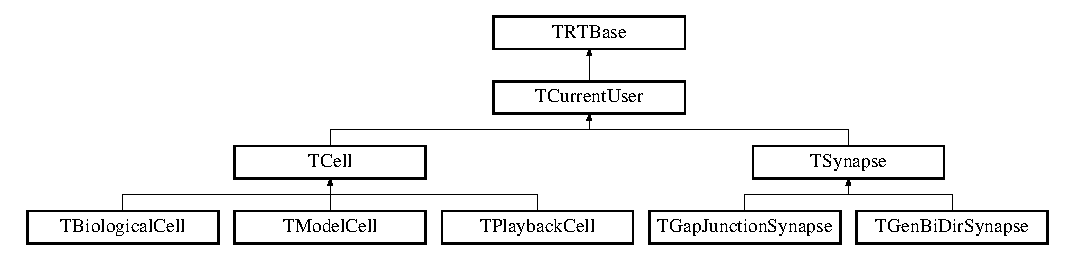
\includegraphics[height=3.047619cm]{class_t_current_user}
\end{center}
\end{figure}
\subsection*{Public Member Functions}
\begin{DoxyCompactItemize}
\item 
virtual const \hyperlink{class_t_current}{T\+Current} $\ast$\+\_\+\+\_\+fastcall \hyperlink{class_t_current_user_a79db0c0c69ec346073feb748f28717f4}{Add\+Current} (\hyperlink{class_t_current}{T\+Current} $\ast$const c, \hyperlink{class_t_cell}{T\+Cell} $\ast$const to\+Cell=N\+U\+L\+L)=0
\begin{DoxyCompactList}\small\item\em Adds a \hyperlink{class_t_current}{T\+Current} $\ast$ to the array of currents in derived class. \end{DoxyCompactList}\item 
virtual void \+\_\+\+\_\+fastcall \hyperlink{class_t_current_user_a957583067328b5a251b8d6cacb6ab279}{Remove\+Current} (\hyperlink{class_t_current}{T\+Current} $\ast$c)=0
\begin{DoxyCompactList}\small\item\em Removes current from class. \end{DoxyCompactList}\item 
\hypertarget{class_t_current_user_ae1c34202d2fe001c392fd1485ec4f3a1}{\+\_\+\+\_\+fastcall \hyperlink{class_t_current_user_ae1c34202d2fe001c392fd1485ec4f3a1}{T\+Current\+User} ()}\label{class_t_current_user_ae1c34202d2fe001c392fd1485ec4f3a1}

\begin{DoxyCompactList}\small\item\em Default constructor. \end{DoxyCompactList}\item 
\hypertarget{class_t_current_user_a6644613131515a0b0529b0c9e7facffb}{\+\_\+\+\_\+fastcall \hyperlink{class_t_current_user_a6644613131515a0b0529b0c9e7facffb}{T\+Current\+User} (const std\+::wstring \&name, const bool active)}\label{class_t_current_user_a6644613131515a0b0529b0c9e7facffb}

\begin{DoxyCompactList}\small\item\em Specialized constructor. \end{DoxyCompactList}\item 
\hypertarget{class_t_current_user_a7360161e482e0f8035df59402ac7ec13}{\+\_\+\+\_\+fastcall \hyperlink{class_t_current_user_a7360161e482e0f8035df59402ac7ec13}{T\+Current\+User} (const \hyperlink{class_t_current_user}{T\+Current\+User} \&source)}\label{class_t_current_user_a7360161e482e0f8035df59402ac7ec13}

\begin{DoxyCompactList}\small\item\em copy constructor \end{DoxyCompactList}\item 
\hypertarget{class_t_current_user_a35f78ca5240120864a9371a4cc61c225}{\hyperlink{class_t_current_user}{T\+Current\+User} \& \hyperlink{class_t_current_user_a35f78ca5240120864a9371a4cc61c225}{operator=} (const \hyperlink{class_t_current_user}{T\+Current\+User} \&source)}\label{class_t_current_user_a35f78ca5240120864a9371a4cc61c225}

\begin{DoxyCompactList}\small\item\em overloaded assignment operator \end{DoxyCompactList}\end{DoxyCompactItemize}
\subsection*{Friends}
\begin{DoxyCompactItemize}
\item 
\hypertarget{class_t_current_user_ac98d07dd8f7b70e16ccb9a01abf56b9c}{class \hyperlink{class_t_current_user_ac98d07dd8f7b70e16ccb9a01abf56b9c}{boost\+::serialization\+::access}}\label{class_t_current_user_ac98d07dd8f7b70e16ccb9a01abf56b9c}

\begin{DoxyCompactList}\small\item\em Required for serialization and saving networks to disk. \end{DoxyCompactList}\end{DoxyCompactItemize}
\subsection*{Additional Inherited Members}


\subsection{Detailed Description}
Base class for derived classes such as \hyperlink{class_t_synapse}{T\+Synapse} and \hyperlink{class_t_cell}{T\+Cell} that have T\+Current-\/derived children. 

\begin{DoxyAuthor}{Author}
E. Brady Trexler $<$ebtrexler (at) gothamsci.\+com$>$, 2011 -\/ 2013 
\end{DoxyAuthor}


\subsection{Member Function Documentation}
\hypertarget{class_t_current_user_a79db0c0c69ec346073feb748f28717f4}{\index{T\+Current\+User@{T\+Current\+User}!Add\+Current@{Add\+Current}}
\index{Add\+Current@{Add\+Current}!T\+Current\+User@{T\+Current\+User}}
\subsubsection[{Add\+Current}]{\setlength{\rightskip}{0pt plus 5cm}virtual const {\bf T\+Current}$\ast$ \+\_\+\+\_\+fastcall T\+Current\+User\+::\+Add\+Current (
\begin{DoxyParamCaption}
\item[{{\bf T\+Current} $\ast$const}]{c, }
\item[{{\bf T\+Cell} $\ast$const}]{to\+Cell = {\ttfamily NULL}}
\end{DoxyParamCaption}
)\hspace{0.3cm}{\ttfamily [pure virtual]}}}\label{class_t_current_user_a79db0c0c69ec346073feb748f28717f4}


Adds a \hyperlink{class_t_current}{T\+Current} $\ast$ to the array of currents in derived class. 

Pure virtual --$>$ class is abstract and can only serve as base class derived classes must override and implement


\begin{DoxyParams}{Parameters}
{\em c} & is pointer to \hyperlink{class_t_current}{T\+Current} derived class \\
\hline
{\em to\+Cell} & is a pointer to the cell affected by this current \\
\hline
\end{DoxyParams}


Implemented in \hyperlink{class_t_playback_cell_aa6230016ea05dc27519729aa7bc38c0f}{T\+Playback\+Cell}, \hyperlink{class_t_cell_ad3dc989fecc587656dfc2f8570dfe772}{T\+Cell}, and \hyperlink{class_t_synapse_a40391153a81e8b475c56ba9a9df9fcfc}{T\+Synapse}.

\hypertarget{class_t_current_user_a957583067328b5a251b8d6cacb6ab279}{\index{T\+Current\+User@{T\+Current\+User}!Remove\+Current@{Remove\+Current}}
\index{Remove\+Current@{Remove\+Current}!T\+Current\+User@{T\+Current\+User}}
\subsubsection[{Remove\+Current}]{\setlength{\rightskip}{0pt plus 5cm}virtual void \+\_\+\+\_\+fastcall T\+Current\+User\+::\+Remove\+Current (
\begin{DoxyParamCaption}
\item[{{\bf T\+Current} $\ast$}]{c}
\end{DoxyParamCaption}
)\hspace{0.3cm}{\ttfamily [pure virtual]}}}\label{class_t_current_user_a957583067328b5a251b8d6cacb6ab279}


Removes current from class. 

Pure virtual --$>$ class is abstract and can only serve as base class derived classes must override and implement 

Implemented in \hyperlink{class_t_cell_af0d4c09293bffc70c99f12de3500edc4}{T\+Cell}, and \hyperlink{class_t_synapse_a21516d391133b6be97c4a63320563f0a}{T\+Synapse}.



The documentation for this class was generated from the following files\+:\begin{DoxyCompactItemize}
\item 
R\+T\+\_\+\+Current\+User.\+h\item 
R\+T\+\_\+\+Current\+User.\+cpp\end{DoxyCompactItemize}

\hypertarget{class_t_data_logger}{\section{T\+Data\+Logger Class Reference}
\label{class_t_data_logger}\index{T\+Data\+Logger@{T\+Data\+Logger}}
}


Simulation data logging class.  




{\ttfamily \#include $<$datalogger.\+h$>$}

\subsection*{Public Member Functions}
\begin{DoxyCompactItemize}
\item 
\hypertarget{class_t_data_logger_aa858b1a2ebb24c593ffd447f54e34962}{std\+::ostringstream \& \hyperlink{class_t_data_logger_aa858b1a2ebb24c593ffd447f54e34962}{Get\+Stream} ()}\label{class_t_data_logger_aa858b1a2ebb24c593ffd447f54e34962}

\begin{DoxyCompactList}\small\item\em Returns the internal stream. \end{DoxyCompactList}\item 
\hypertarget{class_t_data_logger_a5f364699ffadaed989b8b0069fecbe6d}{std\+::ostringstream \& {\bfseries Write\+To} (const wchar\+\_\+t $\ast$filename)}\label{class_t_data_logger_a5f364699ffadaed989b8b0069fecbe6d}

\item 
\hypertarget{class_t_data_logger_a4a14dfd82f7839f7a87f471be754b2e5}{std\+::ostringstream \& {\bfseries Reset} ()}\label{class_t_data_logger_a4a14dfd82f7839f7a87f471be754b2e5}

\end{DoxyCompactItemize}
\subsection*{Protected Attributes}
\begin{DoxyCompactItemize}
\item 
\hypertarget{class_t_data_logger_a8e010eed75ef9fc31a3df855e056449e}{std\+::ostringstream {\bfseries os}}\label{class_t_data_logger_a8e010eed75ef9fc31a3df855e056449e}

\end{DoxyCompactItemize}
\subsection*{Friends}
\begin{DoxyCompactItemize}
\item 
\hypertarget{class_t_data_logger_a50ceac6f24eeb145e75822ca7a0bb697}{{\footnotesize template$<$typename T $>$ }\\\hyperlink{class_t_data_logger}{T\+Data\+Logger} \& {\bfseries operator$<$$<$} (\hyperlink{class_t_data_logger}{T\+Data\+Logger} \&logger, const T \&t)}\label{class_t_data_logger_a50ceac6f24eeb145e75822ca7a0bb697}

\item 
\hypertarget{class_t_data_logger_aac169f84ef7aa88fbfe52dfbf93bf987}{\hyperlink{class_t_data_logger}{T\+Data\+Logger} \& {\bfseries operator$<$$<$} (\hyperlink{class_t_data_logger}{T\+Data\+Logger} \&logger, std\+::ostream \&($\ast$pf)(std\+::ostream \&))}\label{class_t_data_logger_aac169f84ef7aa88fbfe52dfbf93bf987}

\end{DoxyCompactItemize}


\subsection{Detailed Description}
Simulation data logging class. 

Class to facilitate logging of model variables to a file for analysis after a run/simulation

\begin{DoxyAuthor}{Author}
E. Brady Trexler $<$ebtrexler (at) gothamsci.\+com$>$, 2011 -\/ 2013 
\end{DoxyAuthor}


The documentation for this class was generated from the following file\+:\begin{DoxyCompactItemize}
\item 
datalogger.\+h\end{DoxyCompactItemize}

\hypertarget{class_t_electrode}{\section{T\+Electrode Class Reference}
\label{class_t_electrode}\index{T\+Electrode@{T\+Electrode}}
}


Base class designed to function as a simple current injecting electrode.  




{\ttfamily \#include $<$R\+T\+\_\+\+Electrode.\+h$>$}

Inheritance diagram for T\+Electrode\+:\begin{figure}[H]
\begin{center}
\leavevmode
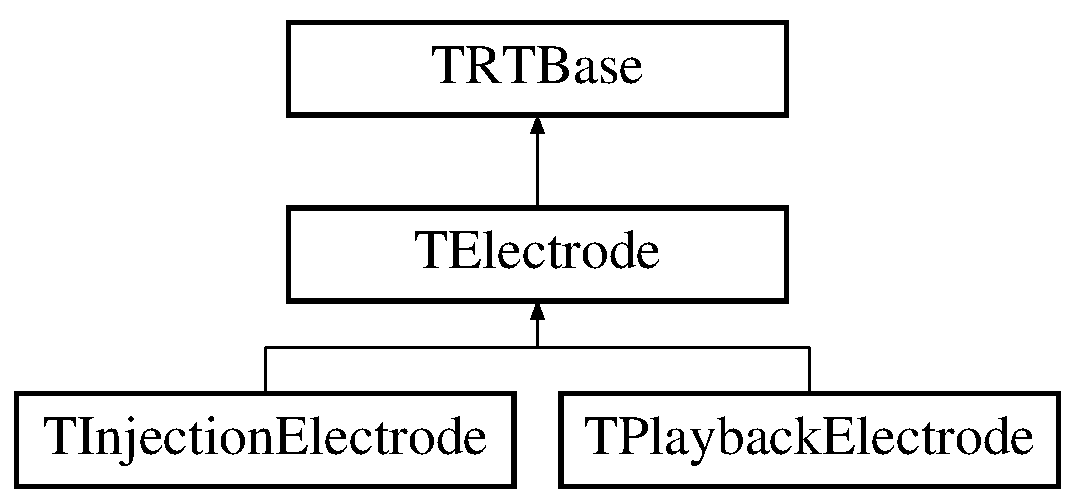
\includegraphics[height=3.000000cm]{class_t_electrode}
\end{center}
\end{figure}
\subsection*{Public Member Functions}
\begin{DoxyCompactItemize}
\item 
\hypertarget{class_t_electrode_ae19b5798e468ff9b6c8519d391e9d2f3}{\hyperlink{class_t_cell}{T\+Cell} $\ast$const \+\_\+\+\_\+fastcall \hyperlink{class_t_electrode_ae19b5798e468ff9b6c8519d391e9d2f3}{Owner} () const }\label{class_t_electrode_ae19b5798e468ff9b6c8519d391e9d2f3}

\begin{DoxyCompactList}\small\item\em Returns the cell \char`\"{}impaled\char`\"{} by this current injecting electrode. \end{DoxyCompactList}\item 
\hypertarget{class_t_electrode_add43f5bb0a835ca9650312de714597db}{double \+\_\+\+\_\+fastcall \hyperlink{class_t_electrode_add43f5bb0a835ca9650312de714597db}{Elapsed\+Time} () const }\label{class_t_electrode_add43f5bb0a835ca9650312de714597db}

\begin{DoxyCompactList}\small\item\em Returns the time since last call to Initialize. \end{DoxyCompactList}\item 
\hypertarget{class_t_electrode_a5f5711cfc03619d470acbe5669e59930}{virtual bool \+\_\+\+\_\+fastcall \hyperlink{class_t_electrode_a5f5711cfc03619d470acbe5669e59930}{Initialize} (bool Reset)=0}\label{class_t_electrode_a5f5711cfc03619d470acbe5669e59930}

\begin{DoxyCompactList}\small\item\em Must override but can call default implementation \hyperlink{class_t_electrode_a5f5711cfc03619d470acbe5669e59930}{T\+Electrode\+::\+Initialize()};. \end{DoxyCompactList}\item 
\hypertarget{class_t_electrode_a3b535fa8d277cf8245f99900fc32ce99}{virtual double \+\_\+\+\_\+fastcall \hyperlink{class_t_electrode_a3b535fa8d277cf8245f99900fc32ce99}{Do\+Update} (double step)=0}\label{class_t_electrode_a3b535fa8d277cf8245f99900fc32ce99}

\begin{DoxyCompactList}\small\item\em Calculates current to inject, must override. \end{DoxyCompactList}\item 
\hypertarget{class_t_electrode_adf2007f7c7031a2d37d83fc87e47a214}{double \+\_\+\+\_\+fastcall \hyperlink{class_t_electrode_adf2007f7c7031a2d37d83fc87e47a214}{Update} (double step)}\label{class_t_electrode_adf2007f7c7031a2d37d83fc87e47a214}

\begin{DoxyCompactList}\small\item\em Updates Elapsed\+Time and calls Do\+Update if Active()==true. \end{DoxyCompactList}\item 
\hypertarget{class_t_electrode_a235d27bb3952e33f3a8e6496e3e2c8f0}{\+\_\+\+\_\+fastcall \hyperlink{class_t_electrode_a235d27bb3952e33f3a8e6496e3e2c8f0}{T\+Electrode} ()}\label{class_t_electrode_a235d27bb3952e33f3a8e6496e3e2c8f0}

\begin{DoxyCompactList}\small\item\em Default constructor. \end{DoxyCompactList}\item 
\hypertarget{class_t_electrode_abf72342739309a48a52037b684517099}{\+\_\+\+\_\+fastcall \hyperlink{class_t_electrode_abf72342739309a48a52037b684517099}{T\+Electrode} (\hyperlink{class_t_cell}{T\+Cell} $\ast$const owner, const std\+::wstring \&name)}\label{class_t_electrode_abf72342739309a48a52037b684517099}

\begin{DoxyCompactList}\small\item\em Specialized constructor. \end{DoxyCompactList}\item 
\hypertarget{class_t_electrode_a18e2f0d510f33cf19a1e62c94ad268b0}{\+\_\+\+\_\+fastcall \hyperlink{class_t_electrode_a18e2f0d510f33cf19a1e62c94ad268b0}{T\+Electrode} (const \hyperlink{class_t_electrode}{T\+Electrode} \&source)}\label{class_t_electrode_a18e2f0d510f33cf19a1e62c94ad268b0}

\begin{DoxyCompactList}\small\item\em Copy constructor. \end{DoxyCompactList}\item 
\hypertarget{class_t_electrode_a6686955e016c2bcea88c70d5b8a03b07}{\hyperlink{class_t_electrode}{T\+Electrode} \& \hyperlink{class_t_electrode_a6686955e016c2bcea88c70d5b8a03b07}{operator=} (const \hyperlink{class_t_electrode}{T\+Electrode} \&source)}\label{class_t_electrode_a6686955e016c2bcea88c70d5b8a03b07}

\begin{DoxyCompactList}\small\item\em Overloaded assignment operator. \end{DoxyCompactList}\end{DoxyCompactItemize}
\subsection*{Friends}
\begin{DoxyCompactItemize}
\item 
\hypertarget{class_t_electrode_ac98d07dd8f7b70e16ccb9a01abf56b9c}{class {\bfseries boost\+::serialization\+::access}}\label{class_t_electrode_ac98d07dd8f7b70e16ccb9a01abf56b9c}

\end{DoxyCompactItemize}
\subsection*{Additional Inherited Members}


\subsection{Detailed Description}
Base class designed to function as a simple current injecting electrode. 

It has virtual Do\+Update(step) that calculates a current based on arbitrary parameters set in derived classes. Do\+Update(step) must be overridden. Descendents of \hyperlink{class_t_electrode}{T\+Electrode} can use its Elapsed\+Time to help define a time dependent waveform.

{\bfseries  --Derived classes must override Do\+Update(step) and return the new current value. }

\begin{DoxyAuthor}{Author}
E. Brady Trexler $<$ebtrexler (at) gothamsci.\+com$>$, 2011 -\/ 2013 
\end{DoxyAuthor}


The documentation for this class was generated from the following files\+:\begin{DoxyCompactItemize}
\item 
R\+T\+\_\+\+Electrode.\+h\item 
R\+T\+\_\+\+Electrode.\+cpp\end{DoxyCompactItemize}

\hypertarget{class_t_gap_junction_current}{\section{T\+Gap\+Junction\+Current Class Reference}
\label{class_t_gap_junction_current}\index{T\+Gap\+Junction\+Current@{T\+Gap\+Junction\+Current}}
}


Implements a current for an electrical synapse.  




{\ttfamily \#include $<$G\+U\+I\+\_\+\+R\+T\+\_\+\+Edit\+\_\+\+G\+J\+Current.\+h$>$}

Inheritance diagram for T\+Gap\+Junction\+Current\+:\begin{figure}[H]
\begin{center}
\leavevmode
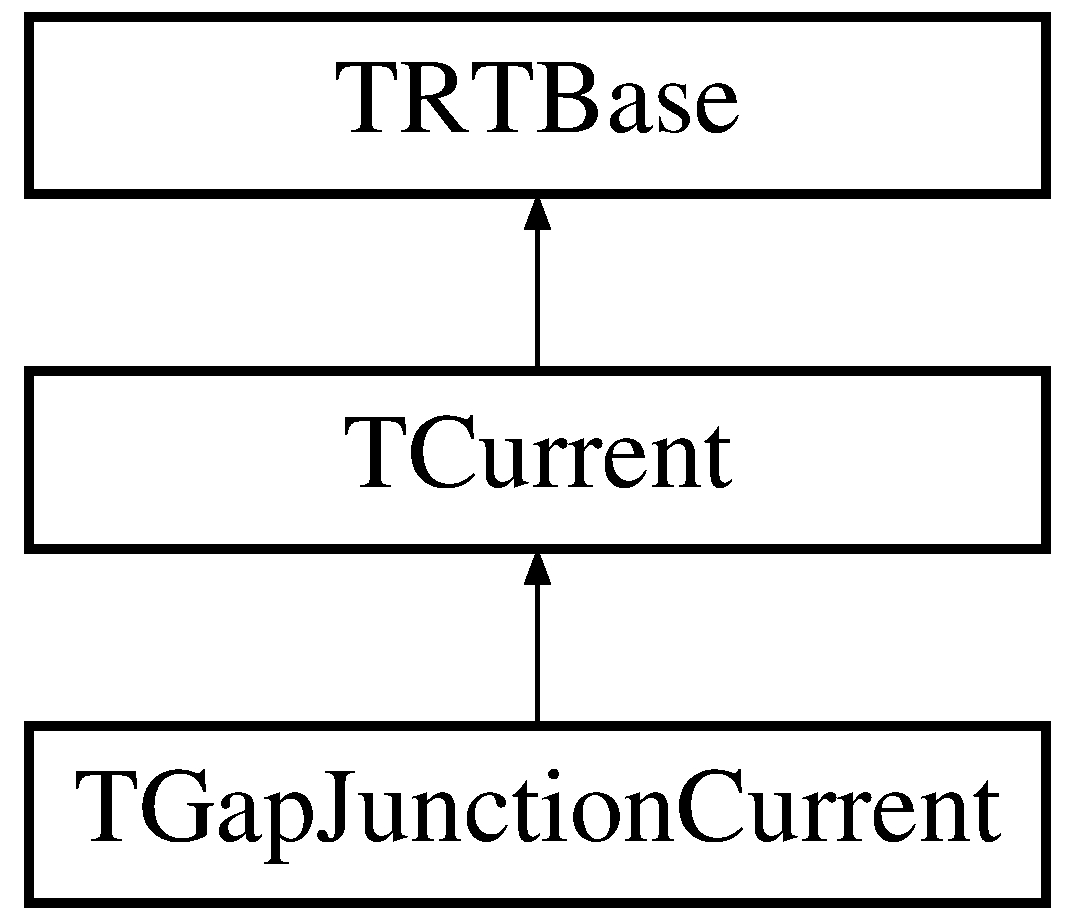
\includegraphics[height=3.000000cm]{class_t_gap_junction_current}
\end{center}
\end{figure}
\subsection*{Public Member Functions}
\begin{DoxyCompactItemize}
\item 
\hypertarget{class_t_gap_junction_current_a919aed5682ef44e406ddce156bd3ba8f}{const double \+\_\+\+\_\+fastcall {\bfseries Gmax} ()}\label{class_t_gap_junction_current_a919aed5682ef44e406ddce156bd3ba8f}

\item 
\hypertarget{class_t_gap_junction_current_a040d4dc75f830644d35ea750e3b62d9e}{void \+\_\+\+\_\+fastcall {\bfseries Set\+Gmax} (double set)}\label{class_t_gap_junction_current_a040d4dc75f830644d35ea750e3b62d9e}

\item 
virtual double \+\_\+\+\_\+fastcall \hyperlink{class_t_gap_junction_current_afe17510f53a732d0499ea704433d69a3}{Do\+Update} (double step, double Vpre, double Vpost, std\+::vector$<$ double $>$ \&params)
\begin{DoxyCompactList}\small\item\em Override in derived classes to implement calculations. \end{DoxyCompactList}\item 
\hypertarget{class_t_gap_junction_current_a27c5c0af154986ba413247df1eb1f8b1}{virtual void \+\_\+\+\_\+fastcall \hyperlink{class_t_gap_junction_current_a27c5c0af154986ba413247df1eb1f8b1}{Populate\+Edit\+Form} ()}\label{class_t_gap_junction_current_a27c5c0af154986ba413247df1eb1f8b1}

\begin{DoxyCompactList}\small\item\em Interface for derived classes, called by G\+U\+I to update V\+C\+L form components. \end{DoxyCompactList}\item 
\hypertarget{class_t_gap_junction_current_a5dba9768c2c9dcf91617cf906ef53bda}{virtual bool \+\_\+\+\_\+fastcall \hyperlink{class_t_gap_junction_current_a5dba9768c2c9dcf91617cf906ef53bda}{Validate\+Edit\+Form} ()}\label{class_t_gap_junction_current_a5dba9768c2c9dcf91617cf906ef53bda}

\begin{DoxyCompactList}\small\item\em Interface for derived classes, called by G\+U\+I to read V\+C\+L form values. \end{DoxyCompactList}\item 
virtual void $\ast$const \+\_\+\+\_\+fastcall \hyperlink{class_t_gap_junction_current_a778ffd1b6c6d72562ad03fa42ef6b55f}{Get\+Edit\+Form} ()
\item 
virtual bool \+\_\+\+\_\+fastcall \hyperlink{class_t_gap_junction_current_a1cc5bf812766be4c91a656aef30c9cfd}{Initialize} (bool Reset)
\begin{DoxyCompactList}\small\item\em Sets Elapsed\+Time to zero. Must be called before first Update. \end{DoxyCompactList}\item 
virtual const std\+::wstring \\*
\&\+\_\+\+\_\+fastcall \hyperlink{class_t_gap_junction_current_af3f5986036ba62eb9d4441e72ccff617}{Class\+Key} () const 
\begin{DoxyCompactList}\small\item\em Returns string used to register class with factory. \end{DoxyCompactList}\item 
\hypertarget{class_t_gap_junction_current_a7b9831ba7c1a350ed719c01f45d8e87f}{\+\_\+\+\_\+fastcall \hyperlink{class_t_gap_junction_current_a7b9831ba7c1a350ed719c01f45d8e87f}{T\+Gap\+Junction\+Current} ()}\label{class_t_gap_junction_current_a7b9831ba7c1a350ed719c01f45d8e87f}

\begin{DoxyCompactList}\small\item\em Default Constructor. \end{DoxyCompactList}\item 
\hypertarget{class_t_gap_junction_current_afcda6e38e4703cf4d6cee205aff8b379}{\+\_\+\+\_\+fastcall \hyperlink{class_t_gap_junction_current_afcda6e38e4703cf4d6cee205aff8b379}{T\+Gap\+Junction\+Current} (\hyperlink{class_t_current_user}{T\+Current\+User} $\ast$owner, const std\+::wstring \&name)}\label{class_t_gap_junction_current_afcda6e38e4703cf4d6cee205aff8b379}

\begin{DoxyCompactList}\small\item\em Specialized Constructor 2 param. \end{DoxyCompactList}\item 
\hypertarget{class_t_gap_junction_current_a41a9c4ad281f266b6d09772d558e2308}{\+\_\+\+\_\+fastcall \hyperlink{class_t_gap_junction_current_a41a9c4ad281f266b6d09772d558e2308}{T\+Gap\+Junction\+Current} (const std\+::wstring \&name)}\label{class_t_gap_junction_current_a41a9c4ad281f266b6d09772d558e2308}

\begin{DoxyCompactList}\small\item\em Specialized Constructor 1 param. \end{DoxyCompactList}\item 
\hypertarget{class_t_gap_junction_current_affe7bbea52d44aa0b6b9bc39df1dcfac}{\+\_\+\+\_\+fastcall \hyperlink{class_t_gap_junction_current_affe7bbea52d44aa0b6b9bc39df1dcfac}{T\+Gap\+Junction\+Current} (const \hyperlink{class_t_gap_junction_current}{T\+Gap\+Junction\+Current} \&source)}\label{class_t_gap_junction_current_affe7bbea52d44aa0b6b9bc39df1dcfac}

\begin{DoxyCompactList}\small\item\em copy constructor \end{DoxyCompactList}\item 
\hypertarget{class_t_gap_junction_current_ac2de0534921e92e81b188fca317f01a4}{\hyperlink{class_t_gap_junction_current}{T\+Gap\+Junction\+Current} \& \hyperlink{class_t_gap_junction_current_ac2de0534921e92e81b188fca317f01a4}{operator=} (const \hyperlink{class_t_gap_junction_current}{T\+Gap\+Junction\+Current} \&source)}\label{class_t_gap_junction_current_ac2de0534921e92e81b188fca317f01a4}

\begin{DoxyCompactList}\small\item\em overloaded assignment operator \end{DoxyCompactList}\item 
\hypertarget{class_t_gap_junction_current_a238e55936013f301a51b163678c18651}{virtual void \+\_\+\+\_\+fastcall \hyperlink{class_t_gap_junction_current_a238e55936013f301a51b163678c18651}{Copy\+Params\+From} (const \hyperlink{class_t_current}{T\+Current} $\ast$const source)}\label{class_t_gap_junction_current_a238e55936013f301a51b163678c18651}

\begin{DoxyCompactList}\small\item\em overloaded method for duplicating currents without complete assignment \end{DoxyCompactList}\end{DoxyCompactItemize}
\subsection*{Protected Member Functions}
\begin{DoxyCompactItemize}
\item 
\hypertarget{class_t_gap_junction_current_a0a2cf2b5493b5552a7d9ce831f4a9e7d}{virtual void const \+\_\+\+\_\+fastcall \hyperlink{class_t_gap_junction_current_a0a2cf2b5493b5552a7d9ce831f4a9e7d}{Write\+To\+Stream} (ostream \&stream) const }\label{class_t_gap_junction_current_a0a2cf2b5493b5552a7d9ce831f4a9e7d}

\begin{DoxyCompactList}\small\item\em Writes data members to a stream. \end{DoxyCompactList}\item 
\hypertarget{class_t_gap_junction_current_aabaa3a51eb6a2bb6481283d18150971d}{virtual void const \+\_\+\+\_\+fastcall \hyperlink{class_t_gap_junction_current_aabaa3a51eb6a2bb6481283d18150971d}{Read\+From\+Stream} (istream \&stream)}\label{class_t_gap_junction_current_aabaa3a51eb6a2bb6481283d18150971d}

\begin{DoxyCompactList}\small\item\em Reads data members from a stream. \end{DoxyCompactList}\item 
const void \+\_\+\+\_\+fastcall \hyperlink{class_t_gap_junction_current_a6cf61f4dad13d5c48004d058d70675cb}{Get\+Param\+Log\+Header} (std\+::vector$<$ std\+::string $>$ \&params) const 
\begin{DoxyCompactList}\small\item\em Supplies column names for parameter logging. \end{DoxyCompactList}\end{DoxyCompactItemize}
\subsection*{Friends}
\begin{DoxyCompactItemize}
\item 
\hypertarget{class_t_gap_junction_current_ac98d07dd8f7b70e16ccb9a01abf56b9c}{class {\bfseries boost\+::serialization\+::access}}\label{class_t_gap_junction_current_ac98d07dd8f7b70e16ccb9a01abf56b9c}

\end{DoxyCompactItemize}


\subsection{Detailed Description}
Implements a current for an electrical synapse. 

\begin{DoxyAuthor}{Author}
E. Brady Trexler $<$ebtrexler (at) gothamsci.\+com$>$, 2011 -\/ 2013 
\end{DoxyAuthor}


\subsection{Member Function Documentation}
\hypertarget{class_t_gap_junction_current_af3f5986036ba62eb9d4441e72ccff617}{\index{T\+Gap\+Junction\+Current@{T\+Gap\+Junction\+Current}!Class\+Key@{Class\+Key}}
\index{Class\+Key@{Class\+Key}!T\+Gap\+Junction\+Current@{T\+Gap\+Junction\+Current}}
\subsubsection[{Class\+Key}]{\setlength{\rightskip}{0pt plus 5cm}const std\+::wstring \&\+\_\+\+\_\+fastcall T\+Gap\+Junction\+Current\+::\+Class\+Key (
\begin{DoxyParamCaption}
{}
\end{DoxyParamCaption}
) const\hspace{0.3cm}{\ttfamily [virtual]}}}\label{class_t_gap_junction_current_af3f5986036ba62eb9d4441e72ccff617}


Returns string used to register class with factory. 

Users of class factories must also tell the class the key they used when registering the class. See factory.\+h 

Implements \hyperlink{class_t_r_t_base_a6083fd510cbcb00faa85e5934fc3c18e}{T\+R\+T\+Base}.

\hypertarget{class_t_gap_junction_current_afe17510f53a732d0499ea704433d69a3}{\index{T\+Gap\+Junction\+Current@{T\+Gap\+Junction\+Current}!Do\+Update@{Do\+Update}}
\index{Do\+Update@{Do\+Update}!T\+Gap\+Junction\+Current@{T\+Gap\+Junction\+Current}}
\subsubsection[{Do\+Update}]{\setlength{\rightskip}{0pt plus 5cm}double \+\_\+\+\_\+fastcall T\+Gap\+Junction\+Current\+::\+Do\+Update (
\begin{DoxyParamCaption}
\item[{double}]{step, }
\item[{double}]{Vkin, }
\item[{double}]{Vdrv, }
\item[{std\+::vector$<$ double $>$ \&}]{params}
\end{DoxyParamCaption}
)\hspace{0.3cm}{\ttfamily [virtual]}}}\label{class_t_gap_junction_current_afe17510f53a732d0499ea704433d69a3}


Override in derived classes to implement calculations. 


\begin{DoxyParams}{Parameters}
{\em step} & = milliseconds passed since last call \\
\hline
{\em Vkin} & = voltage governing kinetics of conductance \\
\hline
{\em Vdrv} & = voltage governing ionic flow through conductance \\
\hline
{\em params} & = vector of calculated parameters for logging \\
\hline
\end{DoxyParams}


Implements \hyperlink{class_t_current_a36d89025eb424f6905fef945c9ae4fa7}{T\+Current}.

\hypertarget{class_t_gap_junction_current_a778ffd1b6c6d72562ad03fa42ef6b55f}{\index{T\+Gap\+Junction\+Current@{T\+Gap\+Junction\+Current}!Get\+Edit\+Form@{Get\+Edit\+Form}}
\index{Get\+Edit\+Form@{Get\+Edit\+Form}!T\+Gap\+Junction\+Current@{T\+Gap\+Junction\+Current}}
\subsubsection[{Get\+Edit\+Form}]{\setlength{\rightskip}{0pt plus 5cm}void $\ast$const \+\_\+\+\_\+fastcall T\+Gap\+Junction\+Current\+::\+Get\+Edit\+Form (
\begin{DoxyParamCaption}
{}
\end{DoxyParamCaption}
)\hspace{0.3cm}{\ttfamily [virtual]}}}\label{class_t_gap_junction_current_a778ffd1b6c6d72562ad03fa42ef6b55f}
Interface for derived classes, returns pointer to G\+U\+I object for editing members. Callers must cast pointer to the correct object. 

Implements \hyperlink{class_t_r_t_base_ab83e520005e20ee71f98f3e85e1ee6d4}{T\+R\+T\+Base}.

\hypertarget{class_t_gap_junction_current_a6cf61f4dad13d5c48004d058d70675cb}{\index{T\+Gap\+Junction\+Current@{T\+Gap\+Junction\+Current}!Get\+Param\+Log\+Header@{Get\+Param\+Log\+Header}}
\index{Get\+Param\+Log\+Header@{Get\+Param\+Log\+Header}!T\+Gap\+Junction\+Current@{T\+Gap\+Junction\+Current}}
\subsubsection[{Get\+Param\+Log\+Header}]{\setlength{\rightskip}{0pt plus 5cm}const void \+\_\+\+\_\+fastcall T\+Gap\+Junction\+Current\+::\+Get\+Param\+Log\+Header (
\begin{DoxyParamCaption}
\item[{std\+::vector$<$ std\+::string $>$ \&}]{params}
\end{DoxyParamCaption}
) const\hspace{0.3cm}{\ttfamily [protected]}, {\ttfamily [virtual]}}}\label{class_t_gap_junction_current_a6cf61f4dad13d5c48004d058d70675cb}


Supplies column names for parameter logging. 


\begin{DoxyParams}{Parameters}
{\em params} & = vector of parameter names for logging Override in derived classes to add their parameters to the header \\
\hline
\end{DoxyParams}


Implements \hyperlink{class_t_current_ab49cb51723efade5eec00fa78fad7ad8}{T\+Current}.

\hypertarget{class_t_gap_junction_current_a1cc5bf812766be4c91a656aef30c9cfd}{\index{T\+Gap\+Junction\+Current@{T\+Gap\+Junction\+Current}!Initialize@{Initialize}}
\index{Initialize@{Initialize}!T\+Gap\+Junction\+Current@{T\+Gap\+Junction\+Current}}
\subsubsection[{Initialize}]{\setlength{\rightskip}{0pt plus 5cm}bool \+\_\+\+\_\+fastcall T\+Gap\+Junction\+Current\+::\+Initialize (
\begin{DoxyParamCaption}
\item[{bool}]{reset}
\end{DoxyParamCaption}
)\hspace{0.3cm}{\ttfamily [virtual]}}}\label{class_t_gap_junction_current_a1cc5bf812766be4c91a656aef30c9cfd}


Sets Elapsed\+Time to zero. Must be called before first Update. 


\begin{DoxyParams}{Parameters}
{\em reset} & = flag for derived classes \\
\hline
\end{DoxyParams}


Reimplemented from \hyperlink{class_t_current_a00c70d232ae85a9841d8d07e5770b7bd}{T\+Current}.



The documentation for this class was generated from the following files\+:\begin{DoxyCompactItemize}
\item 
G\+U\+I\+\_\+\+R\+T\+\_\+\+Edit\+\_\+\+G\+J\+Current.\+h\item 
G\+U\+I\+\_\+\+R\+T\+\_\+\+Edit\+\_\+\+G\+J\+Current.\+cpp\end{DoxyCompactItemize}

\hypertarget{class_t_gap_junction_synapse}{\section{T\+Gap\+Junction\+Synapse Class Reference}
\label{class_t_gap_junction_synapse}\index{T\+Gap\+Junction\+Synapse@{T\+Gap\+Junction\+Synapse}}
}


Specialized synapse with two T\+G\+J\+Currents, one for each direction.  


Inheritance diagram for T\+Gap\+Junction\+Synapse\+:\begin{figure}[H]
\begin{center}
\leavevmode
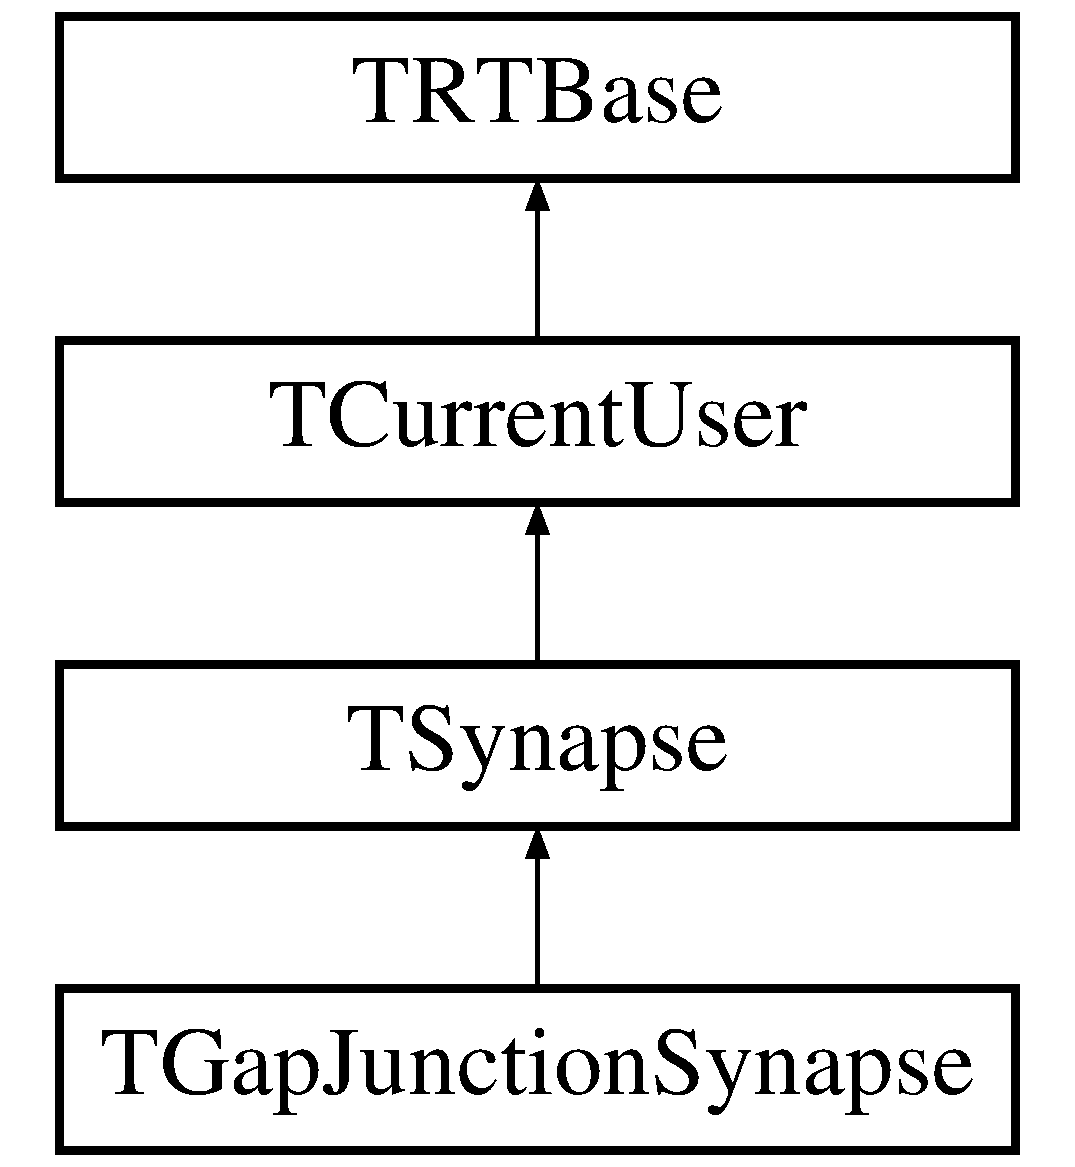
\includegraphics[height=4.000000cm]{class_t_gap_junction_synapse}
\end{center}
\end{figure}
\subsection*{Public Member Functions}
\begin{DoxyCompactItemize}
\item 
\hypertarget{class_t_gap_junction_synapse_ac390f959c2916d6ae385e3f01c796b30}{bool \+\_\+\+\_\+fastcall \hyperlink{class_t_gap_junction_synapse_ac390f959c2916d6ae385e3f01c796b30}{Initialize} (bool Reset)}\label{class_t_gap_junction_synapse_ac390f959c2916d6ae385e3f01c796b30}

\begin{DoxyCompactList}\small\item\em Overrides pure virtual but does nothing. \end{DoxyCompactList}\item 
\hypertarget{class_t_gap_junction_synapse_a989c5cef0289a16b63be18a6300ec64f}{virtual void \+\_\+\+\_\+fastcall \hyperlink{class_t_gap_junction_synapse_a989c5cef0289a16b63be18a6300ec64f}{Populate\+Edit\+Form} ()}\label{class_t_gap_junction_synapse_a989c5cef0289a16b63be18a6300ec64f}

\begin{DoxyCompactList}\small\item\em Interface for derived classes, called by G\+U\+I to update V\+C\+L form components. \end{DoxyCompactList}\item 
\hypertarget{class_t_gap_junction_synapse_af6fba5424b52b27f07553ecfde48f656}{virtual bool \+\_\+\+\_\+fastcall \hyperlink{class_t_gap_junction_synapse_af6fba5424b52b27f07553ecfde48f656}{Validate\+Edit\+Form} ()}\label{class_t_gap_junction_synapse_af6fba5424b52b27f07553ecfde48f656}

\begin{DoxyCompactList}\small\item\em Interface for derived classes, called by G\+U\+I to read V\+C\+L form values. \end{DoxyCompactList}\item 
virtual void $\ast$const \+\_\+\+\_\+fastcall \hyperlink{class_t_gap_junction_synapse_ad1bfccafcf7a340e61d76e9ffa340b63}{Get\+Edit\+Form} ()
\item 
const std\+::wstring \&\+\_\+\+\_\+fastcall \hyperlink{class_t_gap_junction_synapse_abe213c6289ba13e7ca700132fd3f9793}{Class\+Key} () const 
\begin{DoxyCompactList}\small\item\em Returns string used to register class with factory. \end{DoxyCompactList}\item 
\hypertarget{class_t_gap_junction_synapse_aed197bd35857a9933634533872edd262}{\+\_\+\+\_\+fastcall \hyperlink{class_t_gap_junction_synapse_aed197bd35857a9933634533872edd262}{T\+Gap\+Junction\+Synapse} ()}\label{class_t_gap_junction_synapse_aed197bd35857a9933634533872edd262}

\begin{DoxyCompactList}\small\item\em Default Constructor. \end{DoxyCompactList}\item 
\hypertarget{class_t_gap_junction_synapse_a39441e7b583baef4952344ab36bf024b}{\+\_\+\+\_\+fastcall \hyperlink{class_t_gap_junction_synapse_a39441e7b583baef4952344ab36bf024b}{T\+Gap\+Junction\+Synapse} (const std\+::wstring \&name, \hyperlink{class_t_cell}{T\+Cell} $\ast$const pre, \hyperlink{class_t_cell}{T\+Cell} $\ast$const post)}\label{class_t_gap_junction_synapse_a39441e7b583baef4952344ab36bf024b}

\begin{DoxyCompactList}\small\item\em Specialized Constructor. \end{DoxyCompactList}\item 
\hypertarget{class_t_gap_junction_synapse_aad3159733caef0ddcef738d3eb6e8ea2}{\+\_\+\+\_\+fastcall \hyperlink{class_t_gap_junction_synapse_aad3159733caef0ddcef738d3eb6e8ea2}{T\+Gap\+Junction\+Synapse} (const \hyperlink{class_t_gap_junction_synapse}{T\+Gap\+Junction\+Synapse} \&source)}\label{class_t_gap_junction_synapse_aad3159733caef0ddcef738d3eb6e8ea2}

\begin{DoxyCompactList}\small\item\em Copy Constructor. \end{DoxyCompactList}\item 
\hypertarget{class_t_gap_junction_synapse_a5a6165019f4f0040834942b6cb7a4687}{\+\_\+\+\_\+fastcall \hyperlink{class_t_gap_junction_synapse_a5a6165019f4f0040834942b6cb7a4687}{T\+Gap\+Junction\+Synapse} (const \hyperlink{class_t_gap_junction_synapse}{T\+Gap\+Junction\+Synapse} \&source, \hyperlink{class_t_cell}{T\+Cell} $\ast$const new\+Pre, \hyperlink{class_t_cell}{T\+Cell} $\ast$const new\+Post)}\label{class_t_gap_junction_synapse_a5a6165019f4f0040834942b6cb7a4687}

\begin{DoxyCompactList}\small\item\em \char`\"{}duplicate properties with new cells\char`\"{} constructor \end{DoxyCompactList}\item 
\hypertarget{class_t_gap_junction_synapse_ad8c58ce3dd34eb796357d34a6873ade4}{\hyperlink{class_t_gap_junction_synapse}{T\+Gap\+Junction\+Synapse} \& \hyperlink{class_t_gap_junction_synapse_ad8c58ce3dd34eb796357d34a6873ade4}{operator=} (const \hyperlink{class_t_gap_junction_synapse}{T\+Gap\+Junction\+Synapse} \&source)}\label{class_t_gap_junction_synapse_ad8c58ce3dd34eb796357d34a6873ade4}

\begin{DoxyCompactList}\small\item\em Overloaded assignment operator. \end{DoxyCompactList}\end{DoxyCompactItemize}
\subsection*{Friends}
\begin{DoxyCompactItemize}
\item 
\hypertarget{class_t_gap_junction_synapse_ac98d07dd8f7b70e16ccb9a01abf56b9c}{class {\bfseries boost\+::serialization\+::access}}\label{class_t_gap_junction_synapse_ac98d07dd8f7b70e16ccb9a01abf56b9c}

\end{DoxyCompactItemize}
\subsection*{Additional Inherited Members}


\subsection{Detailed Description}
Specialized synapse with two T\+G\+J\+Currents, one for each direction. 

\begin{DoxyAuthor}{Author}
E. Brady Trexler $<$ebtrexler (at) gothamsci.\+com$>$, 2011 -\/ 2013 
\end{DoxyAuthor}


\subsection{Member Function Documentation}
\hypertarget{class_t_gap_junction_synapse_abe213c6289ba13e7ca700132fd3f9793}{\index{T\+Gap\+Junction\+Synapse@{T\+Gap\+Junction\+Synapse}!Class\+Key@{Class\+Key}}
\index{Class\+Key@{Class\+Key}!T\+Gap\+Junction\+Synapse@{T\+Gap\+Junction\+Synapse}}
\subsubsection[{Class\+Key}]{\setlength{\rightskip}{0pt plus 5cm}const std\+::wstring\& \+\_\+\+\_\+fastcall T\+Gap\+Junction\+Synapse\+::\+Class\+Key (
\begin{DoxyParamCaption}
{}
\end{DoxyParamCaption}
) const\hspace{0.3cm}{\ttfamily [inline]}, {\ttfamily [virtual]}}}\label{class_t_gap_junction_synapse_abe213c6289ba13e7ca700132fd3f9793}


Returns string used to register class with factory. 

Users of class factories must also tell the class the key they used when registering the class. See factory.\+h 

Implements \hyperlink{class_t_r_t_base_a6083fd510cbcb00faa85e5934fc3c18e}{T\+R\+T\+Base}.

\hypertarget{class_t_gap_junction_synapse_ad1bfccafcf7a340e61d76e9ffa340b63}{\index{T\+Gap\+Junction\+Synapse@{T\+Gap\+Junction\+Synapse}!Get\+Edit\+Form@{Get\+Edit\+Form}}
\index{Get\+Edit\+Form@{Get\+Edit\+Form}!T\+Gap\+Junction\+Synapse@{T\+Gap\+Junction\+Synapse}}
\subsubsection[{Get\+Edit\+Form}]{\setlength{\rightskip}{0pt plus 5cm}virtual void$\ast$ const \+\_\+\+\_\+fastcall T\+Gap\+Junction\+Synapse\+::\+Get\+Edit\+Form (
\begin{DoxyParamCaption}
{}
\end{DoxyParamCaption}
)\hspace{0.3cm}{\ttfamily [inline]}, {\ttfamily [virtual]}}}\label{class_t_gap_junction_synapse_ad1bfccafcf7a340e61d76e9ffa340b63}
Interface for derived classes, returns pointer to G\+U\+I object for editing members. Callers must cast pointer to the correct object. 

Implements \hyperlink{class_t_r_t_base_ab83e520005e20ee71f98f3e85e1ee6d4}{T\+R\+T\+Base}.



The documentation for this class was generated from the following file\+:\begin{DoxyCompactItemize}
\item 
G\+U\+I\+\_\+\+R\+T\+\_\+\+Edit\+\_\+\+G\+J\+Synapse.\+cpp\end{DoxyCompactItemize}

\hypertarget{class_t_gap_junction_synapse_form}{\section{T\+Gap\+Junction\+Synapse\+Form Class Reference}
\label{class_t_gap_junction_synapse_form}\index{T\+Gap\+Junction\+Synapse\+Form@{T\+Gap\+Junction\+Synapse\+Form}}
}


G\+U\+I editor for \hyperlink{class_t_gap_junction_synapse}{T\+Gap\+Junction\+Synapse}.  




{\ttfamily \#include $<$G\+U\+I\+\_\+\+R\+T\+\_\+\+Edit\+\_\+\+G\+J\+Synapse.\+h$>$}

Inheritance diagram for T\+Gap\+Junction\+Synapse\+Form\+:\begin{figure}[H]
\begin{center}
\leavevmode
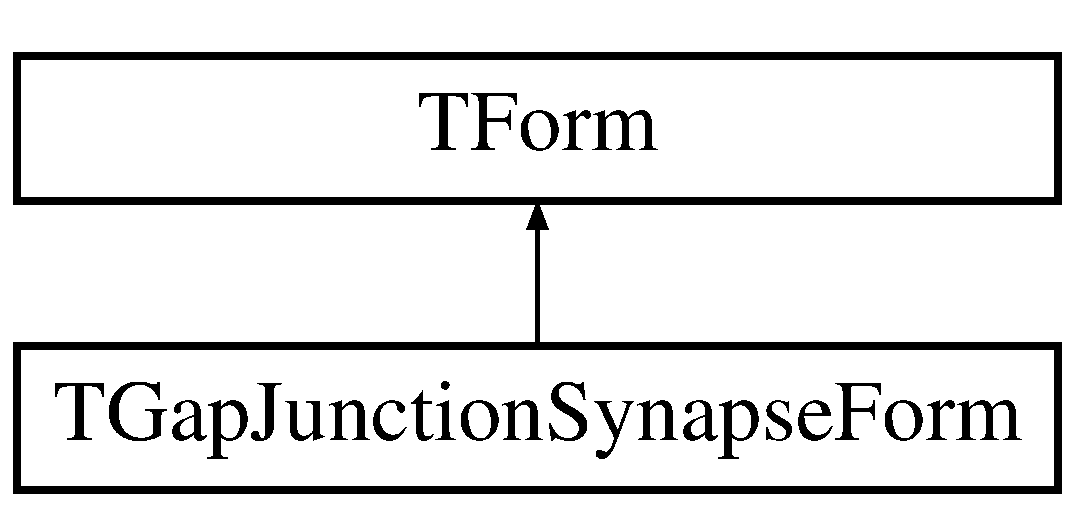
\includegraphics[height=2.000000cm]{class_t_gap_junction_synapse_form}
\end{center}
\end{figure}
\subsection*{Public Member Functions}
\begin{DoxyCompactItemize}
\item 
\hypertarget{class_t_gap_junction_synapse_form_a4ee482a0f47eb61697dd235c4b2d0517}{\+\_\+\+\_\+fastcall {\bfseries T\+Gap\+Junction\+Synapse\+Form} (T\+Component $\ast$Owner)}\label{class_t_gap_junction_synapse_form_a4ee482a0f47eb61697dd235c4b2d0517}

\end{DoxyCompactItemize}
\subsection*{Public Attributes}
\begin{DoxyCompactItemize}
\item 
\hypertarget{class_t_gap_junction_synapse_form_a0b7aef4edb14bd866b8302c7516a45e2}{T\+Group\+Box $\ast$ {\bfseries Group\+Box1}}\label{class_t_gap_junction_synapse_form_a0b7aef4edb14bd866b8302c7516a45e2}

\item 
\hypertarget{class_t_gap_junction_synapse_form_a6b1b55bbe0f87f81ad8cc6ed4c2b0d0c}{T\+Panel $\ast$ {\bfseries Panel1}}\label{class_t_gap_junction_synapse_form_a6b1b55bbe0f87f81ad8cc6ed4c2b0d0c}

\item 
\hypertarget{class_t_gap_junction_synapse_form_a24b399fcc515a4df0c78f98985561bb5}{T\+Group\+Box $\ast$ {\bfseries Group\+Box2}}\label{class_t_gap_junction_synapse_form_a24b399fcc515a4df0c78f98985561bb5}

\item 
\hypertarget{class_t_gap_junction_synapse_form_a63a81abf58ffed566dacd8a285ede1e2}{T\+Panel $\ast$ {\bfseries Panel2}}\label{class_t_gap_junction_synapse_form_a63a81abf58ffed566dacd8a285ede1e2}

\item 
\hypertarget{class_t_gap_junction_synapse_form_af3abdda14fac4735ed075a15730b847a}{\hyperlink{class_t_g_j_current_form}{T\+G\+J\+Current\+Form} $\ast$ {\bfseries Pre\+To\+Post\+Form}}\label{class_t_gap_junction_synapse_form_af3abdda14fac4735ed075a15730b847a}

\item 
\hypertarget{class_t_gap_junction_synapse_form_a336e0fd04c208767a9ab1b087a958230}{\hyperlink{class_t_g_j_current_form}{T\+G\+J\+Current\+Form} $\ast$ {\bfseries Post\+To\+Pre\+Form}}\label{class_t_gap_junction_synapse_form_a336e0fd04c208767a9ab1b087a958230}

\end{DoxyCompactItemize}


\subsection{Detailed Description}
G\+U\+I editor for \hyperlink{class_t_gap_junction_synapse}{T\+Gap\+Junction\+Synapse}. 

\begin{DoxyAuthor}{Author}
E. Brady Trexler $<$ebtrexler (at) gothamsci.\+com$>$, 2011 -\/ 2013 
\end{DoxyAuthor}


The documentation for this class was generated from the following files\+:\begin{DoxyCompactItemize}
\item 
G\+U\+I\+\_\+\+R\+T\+\_\+\+Edit\+\_\+\+G\+J\+Synapse.\+h\item 
G\+U\+I\+\_\+\+R\+T\+\_\+\+Edit\+\_\+\+G\+J\+Synapse.\+cpp\end{DoxyCompactItemize}

\hypertarget{class_t_gen_bi_dir_synapse}{\section{T\+Gen\+Bi\+Dir\+Synapse Class Reference}
\label{class_t_gen_bi_dir_synapse}\index{T\+Gen\+Bi\+Dir\+Synapse@{T\+Gen\+Bi\+Dir\+Synapse}}
}


Implements a bidirectional synapse between two cells.  


Inheritance diagram for T\+Gen\+Bi\+Dir\+Synapse\+:\begin{figure}[H]
\begin{center}
\leavevmode
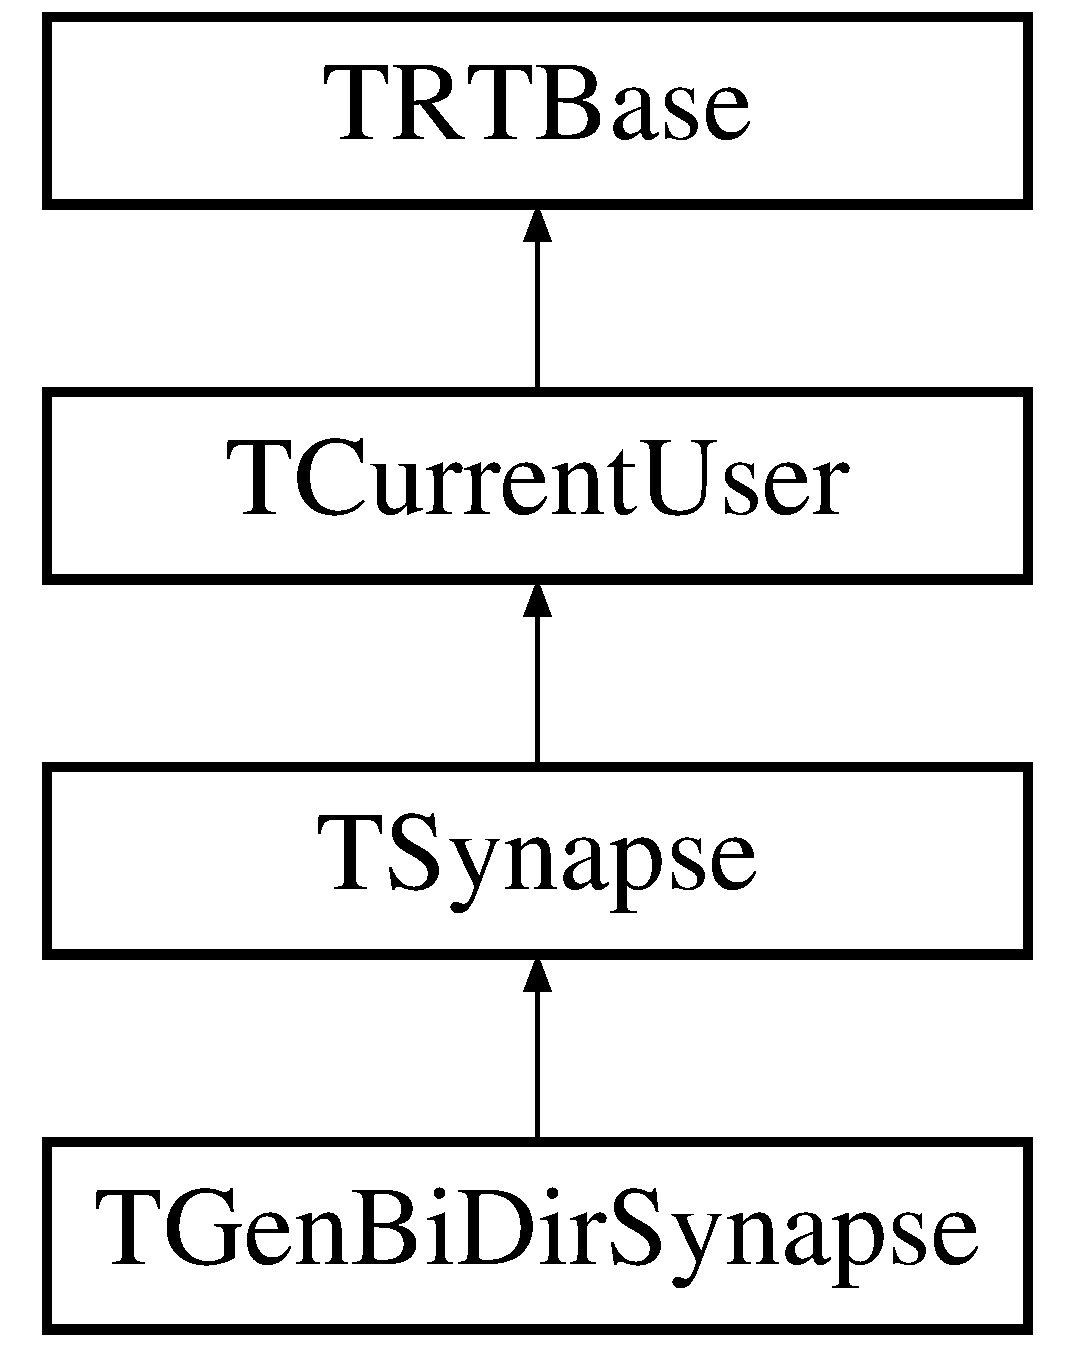
\includegraphics[height=4.000000cm]{class_t_gen_bi_dir_synapse}
\end{center}
\end{figure}
\subsection*{Public Member Functions}
\begin{DoxyCompactItemize}
\item 
\hypertarget{class_t_gen_bi_dir_synapse_a8fa1e97923bdd2c10c300994bd669bfe}{bool \+\_\+\+\_\+fastcall \hyperlink{class_t_gen_bi_dir_synapse_a8fa1e97923bdd2c10c300994bd669bfe}{Initialize} (bool Reset)}\label{class_t_gen_bi_dir_synapse_a8fa1e97923bdd2c10c300994bd669bfe}

\begin{DoxyCompactList}\small\item\em Overrides pure virtual but does nothing. \end{DoxyCompactList}\item 
\hypertarget{class_t_gen_bi_dir_synapse_a372a2931ff3b8fff61c1d61ffdf9ecf1}{virtual void \+\_\+\+\_\+fastcall \hyperlink{class_t_gen_bi_dir_synapse_a372a2931ff3b8fff61c1d61ffdf9ecf1}{Populate\+Edit\+Form} ()}\label{class_t_gen_bi_dir_synapse_a372a2931ff3b8fff61c1d61ffdf9ecf1}

\begin{DoxyCompactList}\small\item\em Interface for derived classes, called by G\+U\+I to update V\+C\+L form components. \end{DoxyCompactList}\item 
\hypertarget{class_t_gen_bi_dir_synapse_ae0a649033ee575e0d0dc0166db02214a}{virtual bool \+\_\+\+\_\+fastcall \hyperlink{class_t_gen_bi_dir_synapse_ae0a649033ee575e0d0dc0166db02214a}{Validate\+Edit\+Form} ()}\label{class_t_gen_bi_dir_synapse_ae0a649033ee575e0d0dc0166db02214a}

\begin{DoxyCompactList}\small\item\em Interface for derived classes, called by G\+U\+I to read V\+C\+L form values. \end{DoxyCompactList}\item 
virtual void $\ast$const \+\_\+\+\_\+fastcall \hyperlink{class_t_gen_bi_dir_synapse_ada612e93b0d7a24ea55201e364bdf7cd}{Get\+Edit\+Form} ()
\item 
const std\+::wstring \&\+\_\+\+\_\+fastcall \hyperlink{class_t_gen_bi_dir_synapse_a7a704a5acb3ec4a36487a762fe87f784}{Class\+Key} () const 
\begin{DoxyCompactList}\small\item\em Returns string used to register class with factory. \end{DoxyCompactList}\item 
\hypertarget{class_t_gen_bi_dir_synapse_a9c9ddea96dcb18cfe9f47ae5c5cae29b}{\+\_\+\+\_\+fastcall \hyperlink{class_t_gen_bi_dir_synapse_a9c9ddea96dcb18cfe9f47ae5c5cae29b}{T\+Gen\+Bi\+Dir\+Synapse} ()}\label{class_t_gen_bi_dir_synapse_a9c9ddea96dcb18cfe9f47ae5c5cae29b}

\begin{DoxyCompactList}\small\item\em Default constructor. \end{DoxyCompactList}\item 
\hypertarget{class_t_gen_bi_dir_synapse_ad203d4920f37fb6bd4e1b84d857956f8}{\+\_\+\+\_\+fastcall \hyperlink{class_t_gen_bi_dir_synapse_ad203d4920f37fb6bd4e1b84d857956f8}{T\+Gen\+Bi\+Dir\+Synapse} (const std\+::wstring \&name, \hyperlink{class_t_cell}{T\+Cell} $\ast$const pre, \hyperlink{class_t_cell}{T\+Cell} $\ast$const post)}\label{class_t_gen_bi_dir_synapse_ad203d4920f37fb6bd4e1b84d857956f8}

\begin{DoxyCompactList}\small\item\em Specialized constructor. \end{DoxyCompactList}\item 
\hypertarget{class_t_gen_bi_dir_synapse_a6ea172aa2c8b0ce676caa4f91e52a224}{\+\_\+\+\_\+fastcall \hyperlink{class_t_gen_bi_dir_synapse_a6ea172aa2c8b0ce676caa4f91e52a224}{T\+Gen\+Bi\+Dir\+Synapse} (const \hyperlink{class_t_gen_bi_dir_synapse}{T\+Gen\+Bi\+Dir\+Synapse} \&source)}\label{class_t_gen_bi_dir_synapse_a6ea172aa2c8b0ce676caa4f91e52a224}

\begin{DoxyCompactList}\small\item\em Copy constructor. \end{DoxyCompactList}\item 
\hypertarget{class_t_gen_bi_dir_synapse_afe8e90216eb7cc5c8123216a64788383}{\+\_\+\+\_\+fastcall \hyperlink{class_t_gen_bi_dir_synapse_afe8e90216eb7cc5c8123216a64788383}{T\+Gen\+Bi\+Dir\+Synapse} (const \hyperlink{class_t_gen_bi_dir_synapse}{T\+Gen\+Bi\+Dir\+Synapse} \&source, \hyperlink{class_t_cell}{T\+Cell} $\ast$const new\+Pre, \hyperlink{class_t_cell}{T\+Cell} $\ast$const new\+Post)}\label{class_t_gen_bi_dir_synapse_afe8e90216eb7cc5c8123216a64788383}

\begin{DoxyCompactList}\small\item\em \char`\"{}\+Duplicate properties with new cells\char`\"{} constructor \end{DoxyCompactList}\item 
\hypertarget{class_t_gen_bi_dir_synapse_ad949c89ba1e3ea34ca26c85912669597}{\hyperlink{class_t_gen_bi_dir_synapse}{T\+Gen\+Bi\+Dir\+Synapse} \& \hyperlink{class_t_gen_bi_dir_synapse_ad949c89ba1e3ea34ca26c85912669597}{operator=} (const \hyperlink{class_t_gen_bi_dir_synapse}{T\+Gen\+Bi\+Dir\+Synapse} \&source)}\label{class_t_gen_bi_dir_synapse_ad949c89ba1e3ea34ca26c85912669597}

\begin{DoxyCompactList}\small\item\em Overloaded assignment operator. \end{DoxyCompactList}\end{DoxyCompactItemize}
\subsection*{Friends}
\begin{DoxyCompactItemize}
\item 
\hypertarget{class_t_gen_bi_dir_synapse_ac98d07dd8f7b70e16ccb9a01abf56b9c}{class {\bfseries boost\+::serialization\+::access}}\label{class_t_gen_bi_dir_synapse_ac98d07dd8f7b70e16ccb9a01abf56b9c}

\end{DoxyCompactItemize}
\subsection*{Additional Inherited Members}


\subsection{Detailed Description}
Implements a bidirectional synapse between two cells. 

\begin{DoxyAuthor}{Author}
E. Brady Trexler $<$ebtrexler (at) gothamsci.\+com$>$, 2011 -\/ 2013 
\end{DoxyAuthor}


\subsection{Member Function Documentation}
\hypertarget{class_t_gen_bi_dir_synapse_a7a704a5acb3ec4a36487a762fe87f784}{\index{T\+Gen\+Bi\+Dir\+Synapse@{T\+Gen\+Bi\+Dir\+Synapse}!Class\+Key@{Class\+Key}}
\index{Class\+Key@{Class\+Key}!T\+Gen\+Bi\+Dir\+Synapse@{T\+Gen\+Bi\+Dir\+Synapse}}
\subsubsection[{Class\+Key}]{\setlength{\rightskip}{0pt plus 5cm}const std\+::wstring\& \+\_\+\+\_\+fastcall T\+Gen\+Bi\+Dir\+Synapse\+::\+Class\+Key (
\begin{DoxyParamCaption}
{}
\end{DoxyParamCaption}
) const\hspace{0.3cm}{\ttfamily [inline]}, {\ttfamily [virtual]}}}\label{class_t_gen_bi_dir_synapse_a7a704a5acb3ec4a36487a762fe87f784}


Returns string used to register class with factory. 

Users of class factories must also tell the class the key they used when registering the class. See factory.\+h 

Implements \hyperlink{class_t_r_t_base_a6083fd510cbcb00faa85e5934fc3c18e}{T\+R\+T\+Base}.

\hypertarget{class_t_gen_bi_dir_synapse_ada612e93b0d7a24ea55201e364bdf7cd}{\index{T\+Gen\+Bi\+Dir\+Synapse@{T\+Gen\+Bi\+Dir\+Synapse}!Get\+Edit\+Form@{Get\+Edit\+Form}}
\index{Get\+Edit\+Form@{Get\+Edit\+Form}!T\+Gen\+Bi\+Dir\+Synapse@{T\+Gen\+Bi\+Dir\+Synapse}}
\subsubsection[{Get\+Edit\+Form}]{\setlength{\rightskip}{0pt plus 5cm}virtual void$\ast$ const \+\_\+\+\_\+fastcall T\+Gen\+Bi\+Dir\+Synapse\+::\+Get\+Edit\+Form (
\begin{DoxyParamCaption}
{}
\end{DoxyParamCaption}
)\hspace{0.3cm}{\ttfamily [inline]}, {\ttfamily [virtual]}}}\label{class_t_gen_bi_dir_synapse_ada612e93b0d7a24ea55201e364bdf7cd}
Interface for derived classes, returns pointer to G\+U\+I object for editing members. Callers must cast pointer to the correct object. 

Implements \hyperlink{class_t_r_t_base_ab83e520005e20ee71f98f3e85e1ee6d4}{T\+R\+T\+Base}.



The documentation for this class was generated from the following file\+:\begin{DoxyCompactItemize}
\item 
G\+U\+I\+\_\+\+R\+T\+\_\+\+Edit\+\_\+\+Gen\+Bi\+Dir\+Synapse.\+cpp\end{DoxyCompactItemize}

\hypertarget{class_t_gen_bi_dir_synapse_form}{\section{T\+Gen\+Bi\+Dir\+Synapse\+Form Class Reference}
\label{class_t_gen_bi_dir_synapse_form}\index{T\+Gen\+Bi\+Dir\+Synapse\+Form@{T\+Gen\+Bi\+Dir\+Synapse\+Form}}
}


G\+U\+I editor for \hyperlink{class_t_gen_bi_dir_synapse}{T\+Gen\+Bi\+Dir\+Synapse}.  




{\ttfamily \#include $<$G\+U\+I\+\_\+\+R\+T\+\_\+\+Edit\+\_\+\+Gen\+Bi\+Dir\+Synapse.\+h$>$}

Inheritance diagram for T\+Gen\+Bi\+Dir\+Synapse\+Form\+:\begin{figure}[H]
\begin{center}
\leavevmode
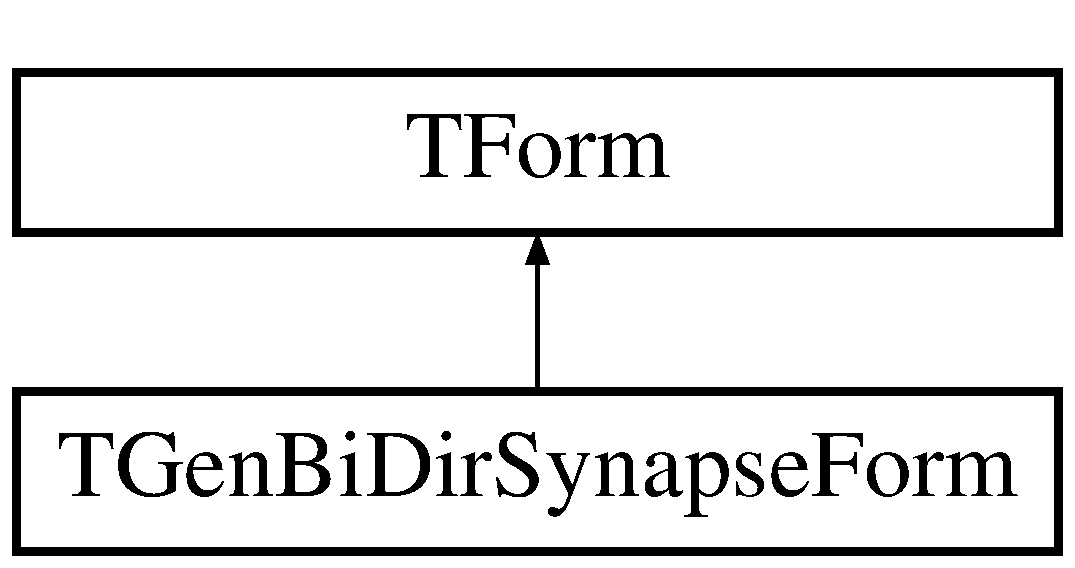
\includegraphics[height=2.000000cm]{class_t_gen_bi_dir_synapse_form}
\end{center}
\end{figure}
\subsection*{Public Member Functions}
\begin{DoxyCompactItemize}
\item 
\hypertarget{class_t_gen_bi_dir_synapse_form_ac04375e74b45855f22ebd0b9ee71b39a}{\+\_\+\+\_\+fastcall {\bfseries T\+Gen\+Bi\+Dir\+Synapse\+Form} (T\+Component $\ast$Owner)}\label{class_t_gen_bi_dir_synapse_form_ac04375e74b45855f22ebd0b9ee71b39a}

\end{DoxyCompactItemize}
\subsection*{Public Attributes}
\begin{DoxyCompactItemize}
\item 
\hypertarget{class_t_gen_bi_dir_synapse_form_a747363dcb7341daf908324bf0c54dd70}{T\+Label $\ast$ {\bfseries Label1}}\label{class_t_gen_bi_dir_synapse_form_a747363dcb7341daf908324bf0c54dd70}

\item 
\hypertarget{class_t_gen_bi_dir_synapse_form_a5e693794dc5a8563d042e7aafaa57dfd}{T\+Label $\ast$ {\bfseries Label2}}\label{class_t_gen_bi_dir_synapse_form_a5e693794dc5a8563d042e7aafaa57dfd}

\item 
\hypertarget{class_t_gen_bi_dir_synapse_form_a4a5c5e98b77b14a72c0bdb17b1d5e155}{\hyperlink{class_t_gen_bi_dir_synapse}{T\+Gen\+Bi\+Dir\+Synapse} $\ast$ {\bfseries Gen\+Bi\+Dir\+Synapse}}\label{class_t_gen_bi_dir_synapse_form_a4a5c5e98b77b14a72c0bdb17b1d5e155}

\end{DoxyCompactItemize}


\subsection{Detailed Description}
G\+U\+I editor for \hyperlink{class_t_gen_bi_dir_synapse}{T\+Gen\+Bi\+Dir\+Synapse}. 

\begin{DoxyAuthor}{Author}
E. Brady Trexler $<$ebtrexler (at) gothamsci.\+com$>$, 2011 -\/ 2013 
\end{DoxyAuthor}


The documentation for this class was generated from the following files\+:\begin{DoxyCompactItemize}
\item 
G\+U\+I\+\_\+\+R\+T\+\_\+\+Edit\+\_\+\+Gen\+Bi\+Dir\+Synapse.\+h\item 
G\+U\+I\+\_\+\+R\+T\+\_\+\+Edit\+\_\+\+Gen\+Bi\+Dir\+Synapse.\+cpp\end{DoxyCompactItemize}

\hypertarget{class_t_g_j_current_form}{\section{T\+G\+J\+Current\+Form Class Reference}
\label{class_t_g_j_current_form}\index{T\+G\+J\+Current\+Form@{T\+G\+J\+Current\+Form}}
}


G\+U\+I Editor for \hyperlink{class_t_gap_junction_current}{T\+Gap\+Junction\+Current}.  




{\ttfamily \#include $<$G\+U\+I\+\_\+\+R\+T\+\_\+\+Edit\+\_\+\+G\+J\+Current.\+h$>$}

Inheritance diagram for T\+G\+J\+Current\+Form\+:\begin{figure}[H]
\begin{center}
\leavevmode
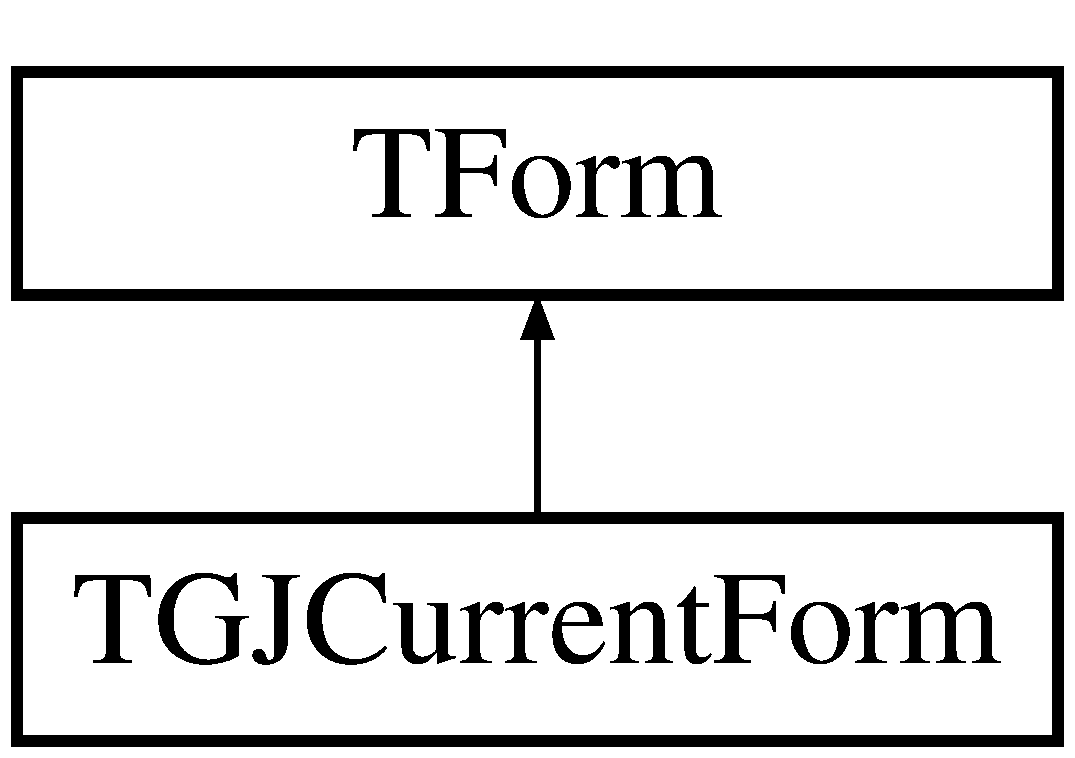
\includegraphics[height=2.000000cm]{class_t_g_j_current_form}
\end{center}
\end{figure}
\subsection*{Public Member Functions}
\begin{DoxyCompactItemize}
\item 
\hypertarget{class_t_g_j_current_form_a87634c2344adc1506087353f7bdd3e91}{void \+\_\+\+\_\+fastcall {\bfseries Edit1\+Key\+Press} (T\+Object $\ast$Sender, wchar\+\_\+t \&Key)}\label{class_t_g_j_current_form_a87634c2344adc1506087353f7bdd3e91}

\item 
\hypertarget{class_t_g_j_current_form_aa1ce2b1f52aec3b0fb1c1bcb78fc0e29}{\+\_\+\+\_\+fastcall {\bfseries T\+G\+J\+Current\+Form} (T\+Component $\ast$Owner)}\label{class_t_g_j_current_form_aa1ce2b1f52aec3b0fb1c1bcb78fc0e29}

\end{DoxyCompactItemize}
\subsection*{Public Attributes}
\begin{DoxyCompactItemize}
\item 
\hypertarget{class_t_g_j_current_form_a404d5114c80a0d9807c20cec17d3adfa}{T\+Label $\ast$ {\bfseries Label1}}\label{class_t_g_j_current_form_a404d5114c80a0d9807c20cec17d3adfa}

\item 
\hypertarget{class_t_g_j_current_form_adaeec92c812d0c2f51452253778974bc}{T\+Edit $\ast$ {\bfseries Edit1}}\label{class_t_g_j_current_form_adaeec92c812d0c2f51452253778974bc}

\item 
\hypertarget{class_t_g_j_current_form_af2b4187cb3820cac1597fddefaa043fd}{T\+Label $\ast$ {\bfseries Label2}}\label{class_t_g_j_current_form_af2b4187cb3820cac1597fddefaa043fd}

\item 
\hypertarget{class_t_g_j_current_form_a8fe2de07f6e52ed84e51ffe434c01627}{\hyperlink{class_t_gap_junction_current}{T\+Gap\+Junction\+Current} $\ast$ {\bfseries G\+J\+Current}}\label{class_t_g_j_current_form_a8fe2de07f6e52ed84e51ffe434c01627}

\end{DoxyCompactItemize}


\subsection{Detailed Description}
G\+U\+I Editor for \hyperlink{class_t_gap_junction_current}{T\+Gap\+Junction\+Current}. 

\begin{DoxyAuthor}{Author}
E. Brady Trexler $<$ebtrexler (at) gothamsci.\+com$>$, 2011 -\/ 2013 
\end{DoxyAuthor}


The documentation for this class was generated from the following files\+:\begin{DoxyCompactItemize}
\item 
G\+U\+I\+\_\+\+R\+T\+\_\+\+Edit\+\_\+\+G\+J\+Current.\+h\item 
G\+U\+I\+\_\+\+R\+T\+\_\+\+Edit\+\_\+\+G\+J\+Current.\+cpp\end{DoxyCompactItemize}

\hypertarget{class_t_g_u_i___circle_perimeter_form}{\section{T\+G\+U\+I\+\_\+\+Circle\+Perimeter\+Form Class Reference}
\label{class_t_g_u_i___circle_perimeter_form}\index{T\+G\+U\+I\+\_\+\+Circle\+Perimeter\+Form@{T\+G\+U\+I\+\_\+\+Circle\+Perimeter\+Form}}
}


G\+U\+I class to display the network as cells arranged evenly around a circle.  




{\ttfamily \#include $<$G\+U\+I\+\_\+\+Circle\+Perimeter\+Editor.\+h$>$}

Inheritance diagram for T\+G\+U\+I\+\_\+\+Circle\+Perimeter\+Form\+:\begin{figure}[H]
\begin{center}
\leavevmode
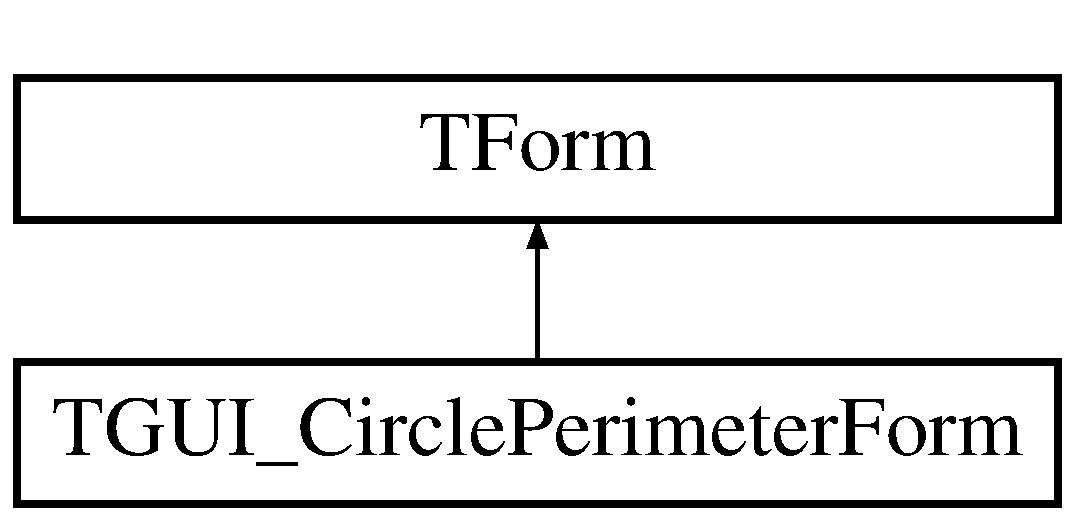
\includegraphics[height=2.000000cm]{class_t_g_u_i___circle_perimeter_form}
\end{center}
\end{figure}
\subsection*{Public Member Functions}
\begin{DoxyCompactItemize}
\item 
\hypertarget{class_t_g_u_i___circle_perimeter_form_af3f4ebc377bfe8579df4930231dd1347}{void \+\_\+\+\_\+fastcall {\bfseries Network\+Paint\+Box32\+Resize} (T\+Object $\ast$Sender)}\label{class_t_g_u_i___circle_perimeter_form_af3f4ebc377bfe8579df4930231dd1347}

\item 
\hypertarget{class_t_g_u_i___circle_perimeter_form_a346821eafb1cc000599d8d4250f97eb8}{void \+\_\+\+\_\+fastcall {\bfseries Network\+Paint\+Box32\+Mouse\+Move} (T\+Object $\ast$Sender, T\+Shift\+State Shift, int X, int Y)}\label{class_t_g_u_i___circle_perimeter_form_a346821eafb1cc000599d8d4250f97eb8}

\item 
\hypertarget{class_t_g_u_i___circle_perimeter_form_ad128d4a37e760d74ebf3091373f3e15e}{void \+\_\+\+\_\+fastcall {\bfseries Network\+Paint\+Box32\+Mouse\+Down} (T\+Object $\ast$Sender, T\+Mouse\+Button Button, T\+Shift\+State Shift, int X, int Y)}\label{class_t_g_u_i___circle_perimeter_form_ad128d4a37e760d74ebf3091373f3e15e}

\item 
\hypertarget{class_t_g_u_i___circle_perimeter_form_aaf875daddf65d68acbc074572ee68596}{void \+\_\+\+\_\+fastcall {\bfseries Form\+Resize} (T\+Object $\ast$Sender)}\label{class_t_g_u_i___circle_perimeter_form_aaf875daddf65d68acbc074572ee68596}

\item 
\hypertarget{class_t_g_u_i___circle_perimeter_form_a09c17990b6741e8455269108ae9f1fa1}{void \+\_\+\+\_\+fastcall {\bfseries Update\+Display} ()}\label{class_t_g_u_i___circle_perimeter_form_a09c17990b6741e8455269108ae9f1fa1}

\item 
\hypertarget{class_t_g_u_i___circle_perimeter_form_ab0bae18e143aeae8728a1cf97f6830b7}{\+\_\+\+\_\+fastcall {\bfseries T\+G\+U\+I\+\_\+\+Circle\+Perimeter\+Form} (T\+Component $\ast$Owner)}\label{class_t_g_u_i___circle_perimeter_form_ab0bae18e143aeae8728a1cf97f6830b7}

\end{DoxyCompactItemize}
\subsection*{Public Attributes}
\begin{DoxyCompactItemize}
\item 
\hypertarget{class_t_g_u_i___circle_perimeter_form_a3f189488faa245c4f4fbe5983c5a24e6}{T\+Paint\+Box32 $\ast$ {\bfseries Network\+Paint\+Box32}}\label{class_t_g_u_i___circle_perimeter_form_a3f189488faa245c4f4fbe5983c5a24e6}

\end{DoxyCompactItemize}


\subsection{Detailed Description}
G\+U\+I class to display the network as cells arranged evenly around a circle. 

\begin{DoxyAuthor}{Author}
E. Brady Trexler $<$ebtrexler (at) gothamsci.\+com$>$, 2011 -\/ 2013 
\end{DoxyAuthor}


The documentation for this class was generated from the following files\+:\begin{DoxyCompactItemize}
\item 
G\+U\+I\+\_\+\+Circle\+Perimeter\+Editor.\+h\item 
G\+U\+I\+\_\+\+Circle\+Perimeter\+Editor.\+cpp\end{DoxyCompactItemize}

\hypertarget{class_t_g_u_i___square_lattice_form}{\section{T\+G\+U\+I\+\_\+\+Square\+Lattice\+Form Class Reference}
\label{class_t_g_u_i___square_lattice_form}\index{T\+G\+U\+I\+\_\+\+Square\+Lattice\+Form@{T\+G\+U\+I\+\_\+\+Square\+Lattice\+Form}}
}


G\+U\+I class to display the network as cells arranged evenly in a grid.  




{\ttfamily \#include $<$G\+U\+I\+\_\+\+Square\+Lattice\+Editor.\+h$>$}

Inheritance diagram for T\+G\+U\+I\+\_\+\+Square\+Lattice\+Form\+:\begin{figure}[H]
\begin{center}
\leavevmode
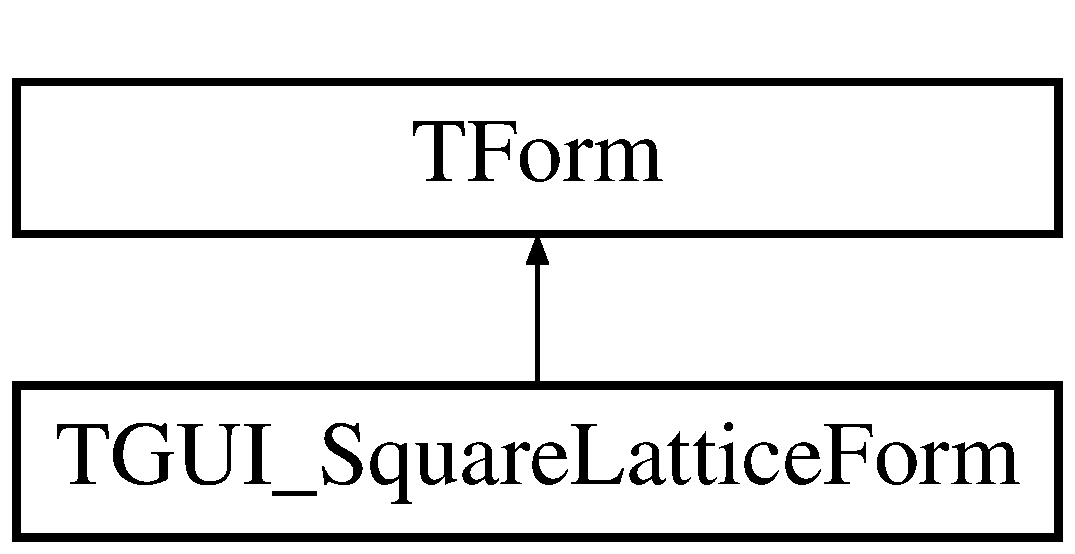
\includegraphics[height=2.000000cm]{class_t_g_u_i___square_lattice_form}
\end{center}
\end{figure}
\subsection*{Public Member Functions}
\begin{DoxyCompactItemize}
\item 
\hypertarget{class_t_g_u_i___square_lattice_form_a4ab9c02ead9e2242ab64920e2acfb0c2}{void \+\_\+\+\_\+fastcall {\bfseries Network\+Paint\+Box32\+Mouse\+Move} (T\+Object $\ast$Sender, T\+Shift\+State Shift, int X, int Y)}\label{class_t_g_u_i___square_lattice_form_a4ab9c02ead9e2242ab64920e2acfb0c2}

\item 
\hypertarget{class_t_g_u_i___square_lattice_form_a3149387afca4cae9338dc3b86b8e090c}{void \+\_\+\+\_\+fastcall {\bfseries Network\+Paint\+Box32\+Mouse\+Down} (T\+Object $\ast$Sender, T\+Mouse\+Button Button, T\+Shift\+State Shift, int X, int Y)}\label{class_t_g_u_i___square_lattice_form_a3149387afca4cae9338dc3b86b8e090c}

\item 
\hypertarget{class_t_g_u_i___square_lattice_form_a3cf1abdd638f931888542a45c7ab2f22}{void \+\_\+\+\_\+fastcall {\bfseries Update\+Display} ()}\label{class_t_g_u_i___square_lattice_form_a3cf1abdd638f931888542a45c7ab2f22}

\item 
\hypertarget{class_t_g_u_i___square_lattice_form_a09b4459eb21fb8c89d48eb0e404fe68d}{\+\_\+\+\_\+fastcall {\bfseries T\+G\+U\+I\+\_\+\+Square\+Lattice\+Form} (T\+Component $\ast$Owner)}\label{class_t_g_u_i___square_lattice_form_a09b4459eb21fb8c89d48eb0e404fe68d}

\end{DoxyCompactItemize}
\subsection*{Public Attributes}
\begin{DoxyCompactItemize}
\item 
\hypertarget{class_t_g_u_i___square_lattice_form_ae5c8a74b0d65b15e50a93748e8e7fd63}{T\+Scroll\+Box $\ast$ {\bfseries Scroll\+Box1}}\label{class_t_g_u_i___square_lattice_form_ae5c8a74b0d65b15e50a93748e8e7fd63}

\item 
\hypertarget{class_t_g_u_i___square_lattice_form_a0c50a6424633ee7c0b083fe5613b16f6}{T\+Paint\+Box32 $\ast$ {\bfseries Network\+Paint\+Box32}}\label{class_t_g_u_i___square_lattice_form_a0c50a6424633ee7c0b083fe5613b16f6}

\end{DoxyCompactItemize}


\subsection{Detailed Description}
G\+U\+I class to display the network as cells arranged evenly in a grid. 

\begin{DoxyAuthor}{Author}
E. Brady Trexler $<$ebtrexler (at) gothamsci.\+com$>$, 2011 -\/ 2013 
\end{DoxyAuthor}


The documentation for this class was generated from the following files\+:\begin{DoxyCompactItemize}
\item 
G\+U\+I\+\_\+\+Square\+Lattice\+Editor.\+h\item 
G\+U\+I\+\_\+\+Square\+Lattice\+Editor.\+cpp\end{DoxyCompactItemize}

\hypertarget{class_t_h_h2_current}{\section{T\+H\+H2\+Current Class Reference}
\label{class_t_h_h2_current}\index{T\+H\+H2\+Current@{T\+H\+H2\+Current}}
}


Implementation of Hodgkin-\/\+Huxley type current with Tohidi-\/\+Nadim shortcuts.  


Inheritance diagram for T\+H\+H2\+Current\+:\begin{figure}[H]
\begin{center}
\leavevmode
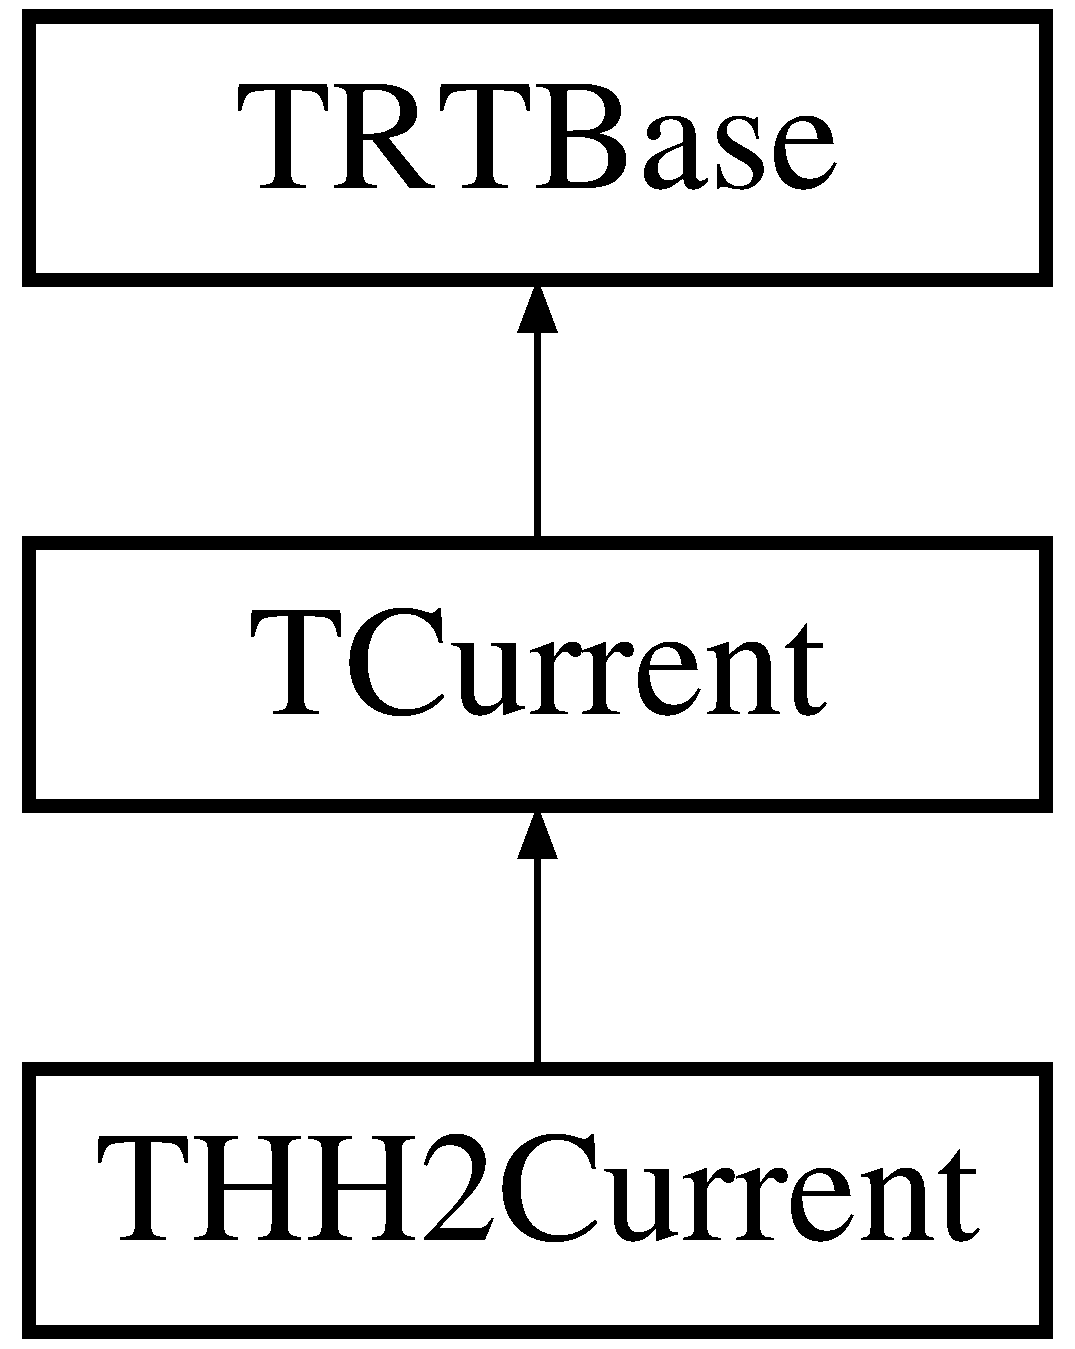
\includegraphics[height=3.000000cm]{class_t_h_h2_current}
\end{center}
\end{figure}
\subsection*{Public Member Functions}
\begin{DoxyCompactItemize}
\item 
\hypertarget{class_t_h_h2_current_a1a74206e21791457b2d88a212c8911b3}{void \+\_\+\+\_\+fastcall {\bfseries Set\+Gmax} (double gmax)}\label{class_t_h_h2_current_a1a74206e21791457b2d88a212c8911b3}

\item 
\hypertarget{class_t_h_h2_current_a57808f5995477893b087c6381c957626}{void \+\_\+\+\_\+fastcall {\bfseries Set\+E} (double erev)}\label{class_t_h_h2_current_a57808f5995477893b087c6381c957626}

\item 
\hypertarget{class_t_h_h2_current_a6c46b837252a9615d2f9cb30949088d7}{void \+\_\+\+\_\+fastcall {\bfseries Set\+Gnoise} (double gnoise)}\label{class_t_h_h2_current_a6c46b837252a9615d2f9cb30949088d7}

\item 
\hypertarget{class_t_h_h2_current_a9bb350baab01c72a7477ec1c354778a4}{double \+\_\+\+\_\+fastcall {\bfseries Get\+Gmax} ()}\label{class_t_h_h2_current_a9bb350baab01c72a7477ec1c354778a4}

\item 
\hypertarget{class_t_h_h2_current_ab37ef56e6ceeea0b0054c79d15a5612a}{double \+\_\+\+\_\+fastcall {\bfseries Get\+E} ()}\label{class_t_h_h2_current_ab37ef56e6ceeea0b0054c79d15a5612a}

\item 
\hypertarget{class_t_h_h2_current_afe78109bb8371fa808f928c7b87dc22e}{double \+\_\+\+\_\+fastcall {\bfseries Get\+Gnoise} ()}\label{class_t_h_h2_current_afe78109bb8371fa808f928c7b87dc22e}

\item 
\hypertarget{class_t_h_h2_current_a2c20ebc20ee04773ee0526cf9562a216}{void \+\_\+\+\_\+fastcall {\bfseries Set\+Gmax2} (double gmax)}\label{class_t_h_h2_current_a2c20ebc20ee04773ee0526cf9562a216}

\item 
\hypertarget{class_t_h_h2_current_a229cb595158f43f4098560d086005ea3}{void \+\_\+\+\_\+fastcall {\bfseries Set\+E2} (double erev)}\label{class_t_h_h2_current_a229cb595158f43f4098560d086005ea3}

\item 
\hypertarget{class_t_h_h2_current_a54f17d790ee8638078a3d07f8eea7b0f}{void \+\_\+\+\_\+fastcall {\bfseries Set\+Gnoise2} (double gnoise)}\label{class_t_h_h2_current_a54f17d790ee8638078a3d07f8eea7b0f}

\item 
\hypertarget{class_t_h_h2_current_ada91730aaaba2b29f580b63ad9b3f240}{double \+\_\+\+\_\+fastcall {\bfseries Get\+Gmax2} ()}\label{class_t_h_h2_current_ada91730aaaba2b29f580b63ad9b3f240}

\item 
\hypertarget{class_t_h_h2_current_ac81e5689edff3393a71cb3e8d0e19e5f}{double \+\_\+\+\_\+fastcall {\bfseries Get\+E2} ()}\label{class_t_h_h2_current_ac81e5689edff3393a71cb3e8d0e19e5f}

\item 
\hypertarget{class_t_h_h2_current_a3eb1393b370fcdb629ca74f6b60d63c7}{double \+\_\+\+\_\+fastcall {\bfseries Get\+Gnoise2} ()}\label{class_t_h_h2_current_a3eb1393b370fcdb629ca74f6b60d63c7}

\item 
bool \+\_\+\+\_\+fastcall \hyperlink{class_t_h_h2_current_aec9a01bd50e5695d3ab16c58e4c4b2a5}{Initialize} (bool Reset)
\begin{DoxyCompactList}\small\item\em Sets Elapsed\+Time to zero. Must be called before first Update. \end{DoxyCompactList}\item 
\hypertarget{class_t_h_h2_current_a8f50ae84c43b83df25bcd203fbe3ebdd}{bool \+\_\+\+\_\+fastcall \hyperlink{class_t_h_h2_current_a8f50ae84c43b83df25bcd203fbe3ebdd}{Restart} (double V)}\label{class_t_h_h2_current_a8f50ae84c43b83df25bcd203fbe3ebdd}

\begin{DoxyCompactList}\small\item\em Initializes kinetic parameters m\+\_\+pre, h\+\_\+pre, n\+\_\+pre, m\+\_\+post, h\+\_\+post, and n\+\_\+post. \end{DoxyCompactList}\item 
const std\+::wstring \&\+\_\+\+\_\+fastcall \hyperlink{class_t_h_h2_current_aede58e5114cd7b8284430badd4c29f3e}{Class\+Key} () const 
\begin{DoxyCompactList}\small\item\em Returns string used to register class with factory. \end{DoxyCompactList}\item 
const void \+\_\+\+\_\+fastcall \hyperlink{class_t_h_h2_current_a3c372c52efdd52caff8dec2387e2378b}{Get\+Param\+Log\+Header} (std\+::vector$<$ std\+::string $>$ \&params) const 
\begin{DoxyCompactList}\small\item\em Supplies column names for parameter logging. \end{DoxyCompactList}\item 
virtual double \+\_\+\+\_\+fastcall \hyperlink{class_t_h_h2_current_a7c7b9b8ce1ce38565abc9caca3d65ab3}{Do\+Update} (double step, double Vkin, double Vdrv, std\+::vector$<$ double $>$ \&params)
\begin{DoxyCompactList}\small\item\em Calculation of H\+H type voltage dependent synaptic current -\/ 3 gates pre and post. \end{DoxyCompactList}\item 
\hypertarget{class_t_h_h2_current_a7434ced3846a8438ab5590a240a6414b}{virtual void \+\_\+\+\_\+fastcall \hyperlink{class_t_h_h2_current_a7434ced3846a8438ab5590a240a6414b}{Populate\+Edit\+Form} ()}\label{class_t_h_h2_current_a7434ced3846a8438ab5590a240a6414b}

\begin{DoxyCompactList}\small\item\em Called by G\+U\+I to synchronize edit form with current values of object params. \end{DoxyCompactList}\item 
\hypertarget{class_t_h_h2_current_aec6192de15f06600102651831fc50676}{bool \hyperlink{class_t_h_h2_current_aec6192de15f06600102651831fc50676}{Kinetic\+Factors\+Validate} (\hyperlink{class_t_h_h_kinetics_factor}{T\+H\+H\+Kinetics\+Factor} \&f, wchar\+\_\+t $\ast$factorname, T\+Value\+List\+Editor $\ast$editor, double \&the\+\_\+exp, wchar\+\_\+t $\ast$exptext)}\label{class_t_h_h2_current_aec6192de15f06600102651831fc50676}

\begin{DoxyCompactList}\small\item\em called by Validate\+Edit\+Form \end{DoxyCompactList}\item 
\hypertarget{class_t_h_h2_current_a298c47cdbab3a2d6054a60d5f433edad}{virtual bool \+\_\+\+\_\+fastcall \hyperlink{class_t_h_h2_current_a298c47cdbab3a2d6054a60d5f433edad}{Validate\+Edit\+Form} ()}\label{class_t_h_h2_current_a298c47cdbab3a2d6054a60d5f433edad}

\begin{DoxyCompactList}\small\item\em Called by G\+U\+I to check if changed values are satisfactory. \end{DoxyCompactList}\item 
\hypertarget{class_t_h_h2_current_a8b78e8e4d6abfe5bac5a8ac256b4e093}{virtual void $\ast$const \+\_\+\+\_\+fastcall \hyperlink{class_t_h_h2_current_a8b78e8e4d6abfe5bac5a8ac256b4e093}{Get\+Edit\+Form} ()}\label{class_t_h_h2_current_a8b78e8e4d6abfe5bac5a8ac256b4e093}

\begin{DoxyCompactList}\small\item\em Returns downcasted T\+H\+H2\+Current\+Form$\ast$ that is used to set values for this object. \end{DoxyCompactList}\item 
\hypertarget{class_t_h_h2_current_ae4d594c506bc6d3eee893604f9aca42b}{\+\_\+\+\_\+fastcall \hyperlink{class_t_h_h2_current_ae4d594c506bc6d3eee893604f9aca42b}{T\+H\+H2\+Current} ()}\label{class_t_h_h2_current_ae4d594c506bc6d3eee893604f9aca42b}

\begin{DoxyCompactList}\small\item\em default constructor \end{DoxyCompactList}\item 
\hypertarget{class_t_h_h2_current_a5fba01d48ccc786ce4328b56019b7c86}{\+\_\+\+\_\+fastcall \hyperlink{class_t_h_h2_current_a5fba01d48ccc786ce4328b56019b7c86}{T\+H\+H2\+Current} (\hyperlink{class_t_current_user}{T\+Current\+User} $\ast$owner, const std\+::wstring \&name)}\label{class_t_h_h2_current_a5fba01d48ccc786ce4328b56019b7c86}

\begin{DoxyCompactList}\small\item\em specialized constructor 2 param \end{DoxyCompactList}\item 
\hypertarget{class_t_h_h2_current_a3886e41d5332d15992aedf3cbfd8d099}{\+\_\+\+\_\+fastcall \hyperlink{class_t_h_h2_current_a3886e41d5332d15992aedf3cbfd8d099}{T\+H\+H2\+Current} (const std\+::wstring \&name)}\label{class_t_h_h2_current_a3886e41d5332d15992aedf3cbfd8d099}

\begin{DoxyCompactList}\small\item\em specialized constructor 1 param \end{DoxyCompactList}\item 
\hypertarget{class_t_h_h2_current_ae4e64c99cbf1340cdc8262c4bccfcbe4}{\+\_\+\+\_\+fastcall \hyperlink{class_t_h_h2_current_ae4e64c99cbf1340cdc8262c4bccfcbe4}{T\+H\+H2\+Current} (const \hyperlink{class_t_h_h2_current}{T\+H\+H2\+Current} \&source)}\label{class_t_h_h2_current_ae4e64c99cbf1340cdc8262c4bccfcbe4}

\begin{DoxyCompactList}\small\item\em copy constructor \end{DoxyCompactList}\item 
\hypertarget{class_t_h_h2_current_a61f3fd3e6cf27271edb52a1aed19be3d}{\hyperlink{class_t_h_h2_current}{T\+H\+H2\+Current} \& \hyperlink{class_t_h_h2_current_a61f3fd3e6cf27271edb52a1aed19be3d}{operator=} (const \hyperlink{class_t_h_h2_current}{T\+H\+H2\+Current} \&source)}\label{class_t_h_h2_current_a61f3fd3e6cf27271edb52a1aed19be3d}

\begin{DoxyCompactList}\small\item\em overloaded assignment operator \end{DoxyCompactList}\item 
\hypertarget{class_t_h_h2_current_a54794ac19d18ec1f9cba53210bca4cf5}{virtual void \+\_\+\+\_\+fastcall \hyperlink{class_t_h_h2_current_a54794ac19d18ec1f9cba53210bca4cf5}{Copy\+Params\+From} (const \hyperlink{class_t_current}{T\+Current} $\ast$const source)}\label{class_t_h_h2_current_a54794ac19d18ec1f9cba53210bca4cf5}

\begin{DoxyCompactList}\small\item\em overloaded method for duplicating currents without complete assignment \end{DoxyCompactList}\end{DoxyCompactItemize}
\subsection*{Public Attributes}
\begin{DoxyCompactItemize}
\item 
\hypertarget{class_t_h_h2_current_a5b74829c0c839cfe13251b3397aa546b}{\+\_\+\+\_\+property double \hyperlink{class_t_h_h2_current_a5b74829c0c839cfe13251b3397aa546b}{p\+\_\+pre} = \{read = F\+\_\+p\+\_\+pre, write = F\+\_\+p\+\_\+pre\}}\label{class_t_h_h2_current_a5b74829c0c839cfe13251b3397aa546b}

\begin{DoxyCompactList}\small\item\em presynaptic activation exponent \end{DoxyCompactList}\item 
\hypertarget{class_t_h_h2_current_a83091d6bba1d4561b0c78d114e3171d5}{\+\_\+\+\_\+property double \hyperlink{class_t_h_h2_current_a83091d6bba1d4561b0c78d114e3171d5}{q\+\_\+pre} = \{read = F\+\_\+q\+\_\+pre, write = F\+\_\+q\+\_\+pre\}}\label{class_t_h_h2_current_a83091d6bba1d4561b0c78d114e3171d5}

\begin{DoxyCompactList}\small\item\em presynaptic inactivation exponent \end{DoxyCompactList}\item 
\hypertarget{class_t_h_h2_current_a6f4db490c5aaa51249cf62c8d385ce61}{\+\_\+\+\_\+property double \hyperlink{class_t_h_h2_current_a6f4db490c5aaa51249cf62c8d385ce61}{r\+\_\+pre} = \{read = F\+\_\+r\+\_\+pre, write = F\+\_\+r\+\_\+pre\}}\label{class_t_h_h2_current_a6f4db490c5aaa51249cf62c8d385ce61}

\begin{DoxyCompactList}\small\item\em presynaptic third param exponent \end{DoxyCompactList}\item 
\hypertarget{class_t_h_h2_current_a26d9308d16a5a093bc03f8c7c038e5fd}{\+\_\+\+\_\+property double \hyperlink{class_t_h_h2_current_a26d9308d16a5a093bc03f8c7c038e5fd}{p\+\_\+post} = \{read = F\+\_\+p\+\_\+post, write = F\+\_\+p\+\_\+post\}}\label{class_t_h_h2_current_a26d9308d16a5a093bc03f8c7c038e5fd}

\begin{DoxyCompactList}\small\item\em postsynaptic activation exponent \end{DoxyCompactList}\item 
\hypertarget{class_t_h_h2_current_af833a70bee269fb98afe6c5106536082}{\+\_\+\+\_\+property double \hyperlink{class_t_h_h2_current_af833a70bee269fb98afe6c5106536082}{q\+\_\+post} = \{read = F\+\_\+q\+\_\+post, write = F\+\_\+q\+\_\+post\}}\label{class_t_h_h2_current_af833a70bee269fb98afe6c5106536082}

\begin{DoxyCompactList}\small\item\em postsynaptic inactivation exponent \end{DoxyCompactList}\item 
\hypertarget{class_t_h_h2_current_afc92a0d4c96ea74bf9d88929b5d7087b}{\+\_\+\+\_\+property double \hyperlink{class_t_h_h2_current_afc92a0d4c96ea74bf9d88929b5d7087b}{r\+\_\+post} = \{read = F\+\_\+r\+\_\+post, write = F\+\_\+r\+\_\+post\}}\label{class_t_h_h2_current_afc92a0d4c96ea74bf9d88929b5d7087b}

\begin{DoxyCompactList}\small\item\em postsynaptic third param exponent \end{DoxyCompactList}\item 
\hypertarget{class_t_h_h2_current_a1a6f4672499821ffb2a1c4f172d9341c}{\+\_\+\+\_\+property double \hyperlink{class_t_h_h2_current_a1a6f4672499821ffb2a1c4f172d9341c}{E} = \{read = Get\+E, write = Set\+E\}}\label{class_t_h_h2_current_a1a6f4672499821ffb2a1c4f172d9341c}

\begin{DoxyCompactList}\small\item\em reversal potential (m\+V) \end{DoxyCompactList}\item 
\hypertarget{class_t_h_h2_current_a297dfe07020e27bff9bf4b4ba520f1e6}{\+\_\+\+\_\+property double \hyperlink{class_t_h_h2_current_a297dfe07020e27bff9bf4b4ba520f1e6}{Gmax} = \{read = Get\+Gmax, write = Set\+Gmax\}}\label{class_t_h_h2_current_a297dfe07020e27bff9bf4b4ba520f1e6}

\begin{DoxyCompactList}\small\item\em mean maximum conductance (u\+S) \end{DoxyCompactList}\item 
\hypertarget{class_t_h_h2_current_a2c75de8014b69355001de11fc3091165}{\+\_\+\+\_\+property double \hyperlink{class_t_h_h2_current_a2c75de8014b69355001de11fc3091165}{Gnoise} = \{read = Get\+Gnoise, write = Set\+Gnoise\}}\label{class_t_h_h2_current_a2c75de8014b69355001de11fc3091165}

\begin{DoxyCompactList}\small\item\em Variation about mean conductance (\%) \end{DoxyCompactList}\item 
\+\_\+\+\_\+property int \hyperlink{class_t_h_h2_current_ae06a0acf968c70a18ad2b9f3a490a131}{Add\+\_\+\+Dont\+\_\+\+Multiply}
\begin{DoxyCompactList}\small\item\em Add conductances rather than multiply. \end{DoxyCompactList}\item 
\hypertarget{class_t_h_h2_current_ad845b98630f025fba797e55a7744c9f0}{\+\_\+\+\_\+property double \hyperlink{class_t_h_h2_current_ad845b98630f025fba797e55a7744c9f0}{E2} = \{read = Get\+E2, write = Set\+E2\}}\label{class_t_h_h2_current_ad845b98630f025fba797e55a7744c9f0}

\begin{DoxyCompactList}\small\item\em reversal potential \#2 (m\+V) \end{DoxyCompactList}\item 
\hypertarget{class_t_h_h2_current_ad518a6e375f6702be1a75b235b1f4b70}{\+\_\+\+\_\+property double \hyperlink{class_t_h_h2_current_ad518a6e375f6702be1a75b235b1f4b70}{Gmax2} = \{read = Get\+Gmax2, write = Set\+Gmax2\}}\label{class_t_h_h2_current_ad518a6e375f6702be1a75b235b1f4b70}

\begin{DoxyCompactList}\small\item\em mean maximum conductance \#2 (u\+S) \end{DoxyCompactList}\item 
\hypertarget{class_t_h_h2_current_a6bebb5c06368b24ce3ff28ac863dca86}{\+\_\+\+\_\+property double \hyperlink{class_t_h_h2_current_a6bebb5c06368b24ce3ff28ac863dca86}{Gnoise2} = \{read = Get\+Gnoise2, write = Set\+Gnoise2\}}\label{class_t_h_h2_current_a6bebb5c06368b24ce3ff28ac863dca86}

\begin{DoxyCompactList}\small\item\em Variation about mean conductance \#2 (\%) \end{DoxyCompactList}\item 
\hypertarget{class_t_h_h2_current_a8062626a434adb2c4176f217785932c4}{\hyperlink{class_t_h_h_kinetics_factor}{T\+H\+H\+Kinetics\+Factor} \hyperlink{class_t_h_h2_current_a8062626a434adb2c4176f217785932c4}{m\+\_\+pre}}\label{class_t_h_h2_current_a8062626a434adb2c4176f217785932c4}

\begin{DoxyCompactList}\small\item\em presynaptic activation kinetic factor \end{DoxyCompactList}\item 
\hypertarget{class_t_h_h2_current_a5401075bf505a9e7f51a9d9458b0a2ed}{\hyperlink{class_t_h_h_kinetics_factor}{T\+H\+H\+Kinetics\+Factor} \hyperlink{class_t_h_h2_current_a5401075bf505a9e7f51a9d9458b0a2ed}{h\+\_\+pre}}\label{class_t_h_h2_current_a5401075bf505a9e7f51a9d9458b0a2ed}

\begin{DoxyCompactList}\small\item\em presynaptic inactivation kinetic factor \end{DoxyCompactList}\item 
\hypertarget{class_t_h_h2_current_a3366e3f7700b429d09e23b97cac0530c}{\hyperlink{class_t_h_h_kinetics_factor}{T\+H\+H\+Kinetics\+Factor} \hyperlink{class_t_h_h2_current_a3366e3f7700b429d09e23b97cac0530c}{n\+\_\+pre}}\label{class_t_h_h2_current_a3366e3f7700b429d09e23b97cac0530c}

\begin{DoxyCompactList}\small\item\em presynaptic third kinetic factor \end{DoxyCompactList}\item 
\hypertarget{class_t_h_h2_current_a5cc7591fe8b43543925b76d6f3324b1d}{\hyperlink{class_t_h_h_kinetics_factor}{T\+H\+H\+Kinetics\+Factor} \hyperlink{class_t_h_h2_current_a5cc7591fe8b43543925b76d6f3324b1d}{m\+\_\+post}}\label{class_t_h_h2_current_a5cc7591fe8b43543925b76d6f3324b1d}

\begin{DoxyCompactList}\small\item\em postsynaptic activation kinetic factor \end{DoxyCompactList}\item 
\hypertarget{class_t_h_h2_current_a3b6c7acdbbcbfb401704407ed6e4777a}{\hyperlink{class_t_h_h_kinetics_factor}{T\+H\+H\+Kinetics\+Factor} \hyperlink{class_t_h_h2_current_a3b6c7acdbbcbfb401704407ed6e4777a}{h\+\_\+post}}\label{class_t_h_h2_current_a3b6c7acdbbcbfb401704407ed6e4777a}

\begin{DoxyCompactList}\small\item\em postsynaptic inactivation kinetic factor \end{DoxyCompactList}\item 
\hypertarget{class_t_h_h2_current_ac875d014e61344e33f89703e65c4d353}{\hyperlink{class_t_h_h_kinetics_factor}{T\+H\+H\+Kinetics\+Factor} \hyperlink{class_t_h_h2_current_ac875d014e61344e33f89703e65c4d353}{n\+\_\+post}}\label{class_t_h_h2_current_ac875d014e61344e33f89703e65c4d353}

\begin{DoxyCompactList}\small\item\em postsynaptic third kinetic factor \end{DoxyCompactList}\end{DoxyCompactItemize}
\subsection*{Protected Member Functions}
\begin{DoxyCompactItemize}
\item 
\hypertarget{class_t_h_h2_current_ac3d319cf12cfa22b570ffa06accc9e88}{virtual void const \+\_\+\+\_\+fastcall \hyperlink{class_t_h_h2_current_ac3d319cf12cfa22b570ffa06accc9e88}{Write\+To\+Stream} (ostream \&stream) const }\label{class_t_h_h2_current_ac3d319cf12cfa22b570ffa06accc9e88}

\begin{DoxyCompactList}\small\item\em Writes data members to a stream. \end{DoxyCompactList}\item 
\hypertarget{class_t_h_h2_current_aab25d91572b98698ede17561073f1e39}{virtual void const \+\_\+\+\_\+fastcall \hyperlink{class_t_h_h2_current_aab25d91572b98698ede17561073f1e39}{Read\+From\+Stream} (istream \&stream)}\label{class_t_h_h2_current_aab25d91572b98698ede17561073f1e39}

\begin{DoxyCompactList}\small\item\em Reads data members from a stream. \end{DoxyCompactList}\end{DoxyCompactItemize}
\subsection*{Friends}
\begin{DoxyCompactItemize}
\item 
\hypertarget{class_t_h_h2_current_ac98d07dd8f7b70e16ccb9a01abf56b9c}{class {\bfseries boost\+::serialization\+::access}}\label{class_t_h_h2_current_ac98d07dd8f7b70e16ccb9a01abf56b9c}

\end{DoxyCompactItemize}


\subsection{Detailed Description}
Implementation of Hodgkin-\/\+Huxley type current with Tohidi-\/\+Nadim shortcuts. 


\begin{DoxyPre}
 Classes \hyperlink{class_t_h_h2_current}{THH2Current} gives ionic current as a function of several kinetic
 parameters and the input voltages V\_kin and V\_drv.  For intrinsic currents
 V\_drv = V\_kin, and for synaptic currents, V\_kin is the voltage of the
 presynaptic cell.\end{DoxyPre}



\begin{DoxyPre}   Computes:               p\_pre      q\_pre      r\_pre
             pre\_gates = m\_pre   *  h\_pre   *  n\_pre\end{DoxyPre}



\begin{DoxyPre}                                     p\_post    q\_post     r\_post
            post\_gates = m\_post  *  h\_post  *  n\_post\end{DoxyPre}



\begin{DoxyPre}            There are two methods to compute the current:\end{DoxyPre}



\begin{DoxyPre}            Multiplication
            I = Gmax * pre\_gates * post\_gates * (V\_drv - E)\end{DoxyPre}



\begin{DoxyPre}            Addition
            I = Gmax * (pre\_gates + post\_gates) * (V\_drv - E)
\end{DoxyPre}


\begin{DoxyAuthor}{Author}
E. Brady Trexler $<$ebtrexler (at) gothamsci.\+com$>$, 2011 -\/ 2013 
\end{DoxyAuthor}


\subsection{Member Function Documentation}
\hypertarget{class_t_h_h2_current_aede58e5114cd7b8284430badd4c29f3e}{\index{T\+H\+H2\+Current@{T\+H\+H2\+Current}!Class\+Key@{Class\+Key}}
\index{Class\+Key@{Class\+Key}!T\+H\+H2\+Current@{T\+H\+H2\+Current}}
\subsubsection[{Class\+Key}]{\setlength{\rightskip}{0pt plus 5cm}const std\+::wstring\& \+\_\+\+\_\+fastcall T\+H\+H2\+Current\+::\+Class\+Key (
\begin{DoxyParamCaption}
{}
\end{DoxyParamCaption}
) const\hspace{0.3cm}{\ttfamily [inline]}, {\ttfamily [virtual]}}}\label{class_t_h_h2_current_aede58e5114cd7b8284430badd4c29f3e}


Returns string used to register class with factory. 

Users of class factories must also tell the class the key they used when registering the class. See factory.\+h 

Implements \hyperlink{class_t_r_t_base_a6083fd510cbcb00faa85e5934fc3c18e}{T\+R\+T\+Base}.

\hypertarget{class_t_h_h2_current_a7c7b9b8ce1ce38565abc9caca3d65ab3}{\index{T\+H\+H2\+Current@{T\+H\+H2\+Current}!Do\+Update@{Do\+Update}}
\index{Do\+Update@{Do\+Update}!T\+H\+H2\+Current@{T\+H\+H2\+Current}}
\subsubsection[{Do\+Update}]{\setlength{\rightskip}{0pt plus 5cm}virtual double \+\_\+\+\_\+fastcall T\+H\+H2\+Current\+::\+Do\+Update (
\begin{DoxyParamCaption}
\item[{double}]{step, }
\item[{double}]{Vkin, }
\item[{double}]{Vdrv, }
\item[{std\+::vector$<$ double $>$ \&}]{params}
\end{DoxyParamCaption}
)\hspace{0.3cm}{\ttfamily [inline]}, {\ttfamily [virtual]}}}\label{class_t_h_h2_current_a7c7b9b8ce1ce38565abc9caca3d65ab3}


Calculation of H\+H type voltage dependent synaptic current -\/ 3 gates pre and post. 


\begin{DoxyPre}
      Computes
                                p\_pre         q\_pre         r\_pre
         pre\_gates =  m\_pre(Vkin) * h\_pre(Vkin) * n\_pre(Vkin)
\begin{DoxyVerb}                     p_post          q_post           r_post
\end{DoxyVerb}

         post\_gates = m\_post(Vdrv)  *  h\_post(Vdrv)  *  n\_post(Vdrv)\end{DoxyPre}



\begin{DoxyPre}      and
         I = Gmax * pre\_gates * post\_gates * (Vdrv - E)
\end{DoxyPre}
 

Implements \hyperlink{class_t_current_a36d89025eb424f6905fef945c9ae4fa7}{T\+Current}.

\hypertarget{class_t_h_h2_current_a3c372c52efdd52caff8dec2387e2378b}{\index{T\+H\+H2\+Current@{T\+H\+H2\+Current}!Get\+Param\+Log\+Header@{Get\+Param\+Log\+Header}}
\index{Get\+Param\+Log\+Header@{Get\+Param\+Log\+Header}!T\+H\+H2\+Current@{T\+H\+H2\+Current}}
\subsubsection[{Get\+Param\+Log\+Header}]{\setlength{\rightskip}{0pt plus 5cm}const void \+\_\+\+\_\+fastcall T\+H\+H2\+Current\+::\+Get\+Param\+Log\+Header (
\begin{DoxyParamCaption}
\item[{std\+::vector$<$ std\+::string $>$ \&}]{params}
\end{DoxyParamCaption}
) const\hspace{0.3cm}{\ttfamily [inline]}, {\ttfamily [virtual]}}}\label{class_t_h_h2_current_a3c372c52efdd52caff8dec2387e2378b}


Supplies column names for parameter logging. 


\begin{DoxyParams}{Parameters}
{\em params} & = vector of parameter names for logging Override in derived classes to add their parameters to the header \\
\hline
\end{DoxyParams}


Implements \hyperlink{class_t_current_ab49cb51723efade5eec00fa78fad7ad8}{T\+Current}.

\hypertarget{class_t_h_h2_current_aec9a01bd50e5695d3ab16c58e4c4b2a5}{\index{T\+H\+H2\+Current@{T\+H\+H2\+Current}!Initialize@{Initialize}}
\index{Initialize@{Initialize}!T\+H\+H2\+Current@{T\+H\+H2\+Current}}
\subsubsection[{Initialize}]{\setlength{\rightskip}{0pt plus 5cm}bool \+\_\+\+\_\+fastcall T\+H\+H2\+Current\+::\+Initialize (
\begin{DoxyParamCaption}
\item[{bool}]{reset}
\end{DoxyParamCaption}
)\hspace{0.3cm}{\ttfamily [inline]}, {\ttfamily [virtual]}}}\label{class_t_h_h2_current_aec9a01bd50e5695d3ab16c58e4c4b2a5}


Sets Elapsed\+Time to zero. Must be called before first Update. 


\begin{DoxyParams}{Parameters}
{\em reset} & = flag for derived classes \\
\hline
\end{DoxyParams}


Reimplemented from \hyperlink{class_t_current_a00c70d232ae85a9841d8d07e5770b7bd}{T\+Current}.



\subsection{Member Data Documentation}
\hypertarget{class_t_h_h2_current_ae06a0acf968c70a18ad2b9f3a490a131}{\index{T\+H\+H2\+Current@{T\+H\+H2\+Current}!Add\+\_\+\+Dont\+\_\+\+Multiply@{Add\+\_\+\+Dont\+\_\+\+Multiply}}
\index{Add\+\_\+\+Dont\+\_\+\+Multiply@{Add\+\_\+\+Dont\+\_\+\+Multiply}!T\+H\+H2\+Current@{T\+H\+H2\+Current}}
\subsubsection[{Add\+\_\+\+Dont\+\_\+\+Multiply}]{\setlength{\rightskip}{0pt plus 5cm}\+\_\+\+\_\+property int T\+H\+H2\+Current\+::\+Add\+\_\+\+Dont\+\_\+\+Multiply}}\label{class_t_h_h2_current_ae06a0acf968c70a18ad2b9f3a490a131}
{\bfseries Initial value\+:}
\begin{DoxyCode}
= \{read = F\_Add\_Dont\_Multiply,
                                                                    write = F\_Add\_Dont\_Multiply\}
\end{DoxyCode}


Add conductances rather than multiply. 



The documentation for this class was generated from the following file\+:\begin{DoxyCompactItemize}
\item 
G\+U\+I\+\_\+\+R\+T\+\_\+\+Edit\+\_\+\+H\+H2\+Current.\+cpp\end{DoxyCompactItemize}

\hypertarget{class_t_h_h2_current_form}{\section{T\+H\+H2\+Current\+Form Class Reference}
\label{class_t_h_h2_current_form}\index{T\+H\+H2\+Current\+Form@{T\+H\+H2\+Current\+Form}}
}


G\+U\+I editor for \hyperlink{class_t_h_h2_current}{T\+H\+H2\+Current}.  




{\ttfamily \#include $<$G\+U\+I\+\_\+\+R\+T\+\_\+\+Edit\+\_\+\+H\+H2\+Current.\+h$>$}

Inheritance diagram for T\+H\+H2\+Current\+Form\+:\begin{figure}[H]
\begin{center}
\leavevmode
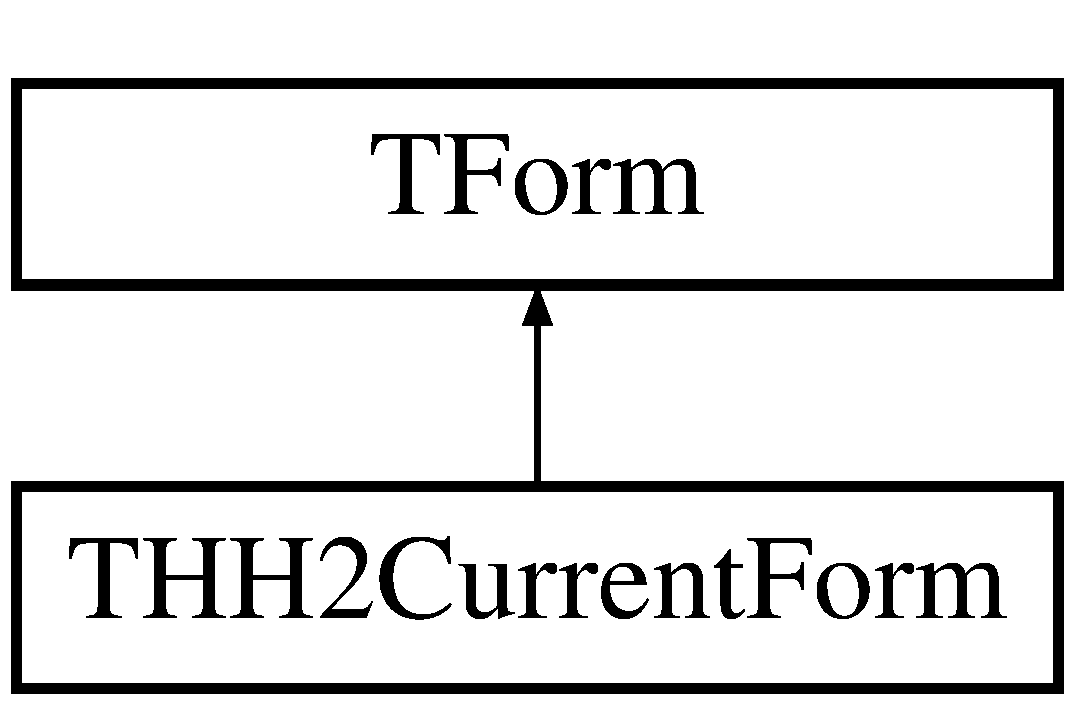
\includegraphics[height=2.000000cm]{class_t_h_h2_current_form}
\end{center}
\end{figure}
\subsection*{Public Member Functions}
\begin{DoxyCompactItemize}
\item 
\hypertarget{class_t_h_h2_current_form_ad93f10ac76f8ff6cc1ee6333775b487f}{void \+\_\+\+\_\+fastcall \hyperlink{class_t_h_h2_current_form_ad93f10ac76f8ff6cc1ee6333775b487f}{Params\+Editors\+\_\+\+Key\+Press} (T\+Object $\ast$Sender, wchar\+\_\+t \&Key)}\label{class_t_h_h2_current_form_ad93f10ac76f8ff6cc1ee6333775b487f}

\begin{DoxyCompactList}\small\item\em Calls Update\+Plots to reflect changes if valid, otherwise no changes accepted. \end{DoxyCompactList}\item 
\hypertarget{class_t_h_h2_current_form_a5f54ce69eef294d3b8e858bd69dca8f0}{void \+\_\+\+\_\+fastcall \hyperlink{class_t_h_h2_current_form_a5f54ce69eef294d3b8e858bd69dca8f0}{Load\+Button\+Click} (T\+Object $\ast$Sender)}\label{class_t_h_h2_current_form_a5f54ce69eef294d3b8e858bd69dca8f0}

\begin{DoxyCompactList}\small\item\em Opens saved parameters from dialog-\/chosen file. \end{DoxyCompactList}\item 
\hypertarget{class_t_h_h2_current_form_a45af940d1fac9b4aa47f363dcc82b576}{void \+\_\+\+\_\+fastcall \hyperlink{class_t_h_h2_current_form_a45af940d1fac9b4aa47f363dcc82b576}{Save\+Button\+Click} (T\+Object $\ast$Sender)}\label{class_t_h_h2_current_form_a45af940d1fac9b4aa47f363dcc82b576}

\begin{DoxyCompactList}\small\item\em Saves parameters to dialog-\/chosen file. \end{DoxyCompactList}\item 
\hypertarget{class_t_h_h2_current_form_a1a95a919832e6ac46f3dbb0d1c34f0ee}{void \+\_\+\+\_\+fastcall {\bfseries Tab\+Control1\+Changing} (T\+Object $\ast$Sender, bool \&Allow\+Change)}\label{class_t_h_h2_current_form_a1a95a919832e6ac46f3dbb0d1c34f0ee}

\item 
\hypertarget{class_t_h_h2_current_form_a460d32fb79ac8386109c3f43af6bc26a}{void \+\_\+\+\_\+fastcall {\bfseries Tab\+Control1\+Change} (T\+Object $\ast$Sender)}\label{class_t_h_h2_current_form_a460d32fb79ac8386109c3f43af6bc26a}

\item 
\hypertarget{class_t_h_h2_current_form_afaaaeff7de4d15315e10f730f2473b13}{void \+\_\+\+\_\+fastcall {\bfseries G\+Calc\+Radio\+Group\+Click} (T\+Object $\ast$Sender)}\label{class_t_h_h2_current_form_afaaaeff7de4d15315e10f730f2473b13}

\item 
\hypertarget{class_t_h_h2_current_form_a28b7fd7d9515c8ef9cd706b9bc8bf435}{void \+\_\+\+\_\+fastcall \hyperlink{class_t_h_h2_current_form_a28b7fd7d9515c8ef9cd706b9bc8bf435}{Update\+Plots} ()}\label{class_t_h_h2_current_form_a28b7fd7d9515c8ef9cd706b9bc8bf435}

\begin{DoxyCompactList}\small\item\em Called when parameter changes need to be reflected in G\+U\+I. \end{DoxyCompactList}\item 
\hypertarget{class_t_h_h2_current_form_ade431854044d6b9454793bb03fbdc727}{\+\_\+\+\_\+fastcall {\bfseries T\+H\+H2\+Current\+Form} (T\+Component $\ast$Owner)}\label{class_t_h_h2_current_form_ade431854044d6b9454793bb03fbdc727}

\end{DoxyCompactItemize}
\subsection*{Public Attributes}
\begin{DoxyCompactItemize}
\item 
\hypertarget{class_t_h_h2_current_form_a80ea7e8f53603b97cdd1b422f096bff3}{T\+Label $\ast$ {\bfseries Label8}}\label{class_t_h_h2_current_form_a80ea7e8f53603b97cdd1b422f096bff3}

\item 
\hypertarget{class_t_h_h2_current_form_abb3915d32903fabaf3370ac91cc561de}{T\+Group\+Box $\ast$ {\bfseries Group\+Box1}}\label{class_t_h_h2_current_form_abb3915d32903fabaf3370ac91cc561de}

\item 
\hypertarget{class_t_h_h2_current_form_a60e4a5d4efdc6e9204db53759f838453}{T\+Panel $\ast$ {\bfseries Panel1}}\label{class_t_h_h2_current_form_a60e4a5d4efdc6e9204db53759f838453}

\item 
\hypertarget{class_t_h_h2_current_form_ac140ffaf73754c043888c43be50ad57a}{T\+Value\+List\+Editor $\ast$ {\bfseries Value\+List\+Editor\+\_\+m}}\label{class_t_h_h2_current_form_ac140ffaf73754c043888c43be50ad57a}

\item 
\hypertarget{class_t_h_h2_current_form_a36293e5f63eb4af935ea686e9b44ab08}{T\+Group\+Box $\ast$ {\bfseries Group\+Box2}}\label{class_t_h_h2_current_form_a36293e5f63eb4af935ea686e9b44ab08}

\item 
\hypertarget{class_t_h_h2_current_form_a0c2aa9683a272b12d0b8cb016c7b5741}{T\+Panel $\ast$ {\bfseries Panel2}}\label{class_t_h_h2_current_form_a0c2aa9683a272b12d0b8cb016c7b5741}

\item 
\hypertarget{class_t_h_h2_current_form_a5ed3717979c2ce49f7934425962d33da}{T\+Value\+List\+Editor $\ast$ {\bfseries Value\+List\+Editor\+\_\+h}}\label{class_t_h_h2_current_form_a5ed3717979c2ce49f7934425962d33da}

\item 
\hypertarget{class_t_h_h2_current_form_a58d2c47b5fb30564ded9469f207627e2}{T\+Multi\+P\+L\+O\+T\+Panel $\ast$ {\bfseries Multi\+P\+L\+O\+T\+Panel1}}\label{class_t_h_h2_current_form_a58d2c47b5fb30564ded9469f207627e2}

\item 
\hypertarget{class_t_h_h2_current_form_a3d0494352a6ddc9cf471867af0c84ed1}{T\+Label $\ast$ {\bfseries Label7}}\label{class_t_h_h2_current_form_a3d0494352a6ddc9cf471867af0c84ed1}

\item 
\hypertarget{class_t_h_h2_current_form_aae3ae64128b421dc85fe359f97da68a8}{T\+Group\+Box $\ast$ {\bfseries Group\+Box3}}\label{class_t_h_h2_current_form_aae3ae64128b421dc85fe359f97da68a8}

\item 
\hypertarget{class_t_h_h2_current_form_aa191c1c9b61cf3ebd3d5b49709e39a68}{T\+Panel $\ast$ {\bfseries Panel3}}\label{class_t_h_h2_current_form_aa191c1c9b61cf3ebd3d5b49709e39a68}

\item 
\hypertarget{class_t_h_h2_current_form_abc28a071680d3b72bfd0814315757168}{T\+Value\+List\+Editor $\ast$ {\bfseries Value\+List\+Editor\+\_\+n}}\label{class_t_h_h2_current_form_abc28a071680d3b72bfd0814315757168}

\item 
\hypertarget{class_t_h_h2_current_form_a7df5d5dcd83a536eafca1a029ca654ea}{T\+Panel $\ast$ {\bfseries Panel4}}\label{class_t_h_h2_current_form_a7df5d5dcd83a536eafca1a029ca654ea}

\item 
\hypertarget{class_t_h_h2_current_form_afea594f233cb89d22ec5e02cca97427a}{T\+Panel $\ast$ {\bfseries Panel5}}\label{class_t_h_h2_current_form_afea594f233cb89d22ec5e02cca97427a}

\item 
\hypertarget{class_t_h_h2_current_form_ac0b573b81c78efd9c56346cc121312f2}{T\+Open\+Dialog $\ast$ {\bfseries Open\+Dialog1}}\label{class_t_h_h2_current_form_ac0b573b81c78efd9c56346cc121312f2}

\item 
\hypertarget{class_t_h_h2_current_form_aa3e4efa388d6450efbba36411b202375}{T\+Save\+Dialog $\ast$ {\bfseries Save\+Dialog1}}\label{class_t_h_h2_current_form_aa3e4efa388d6450efbba36411b202375}

\item 
\hypertarget{class_t_h_h2_current_form_a238fd9c03d8ecc9b48a812ff2c4ecd3b}{T\+Tab\+Control $\ast$ {\bfseries Tab\+Control1}}\label{class_t_h_h2_current_form_a238fd9c03d8ecc9b48a812ff2c4ecd3b}

\item 
\hypertarget{class_t_h_h2_current_form_a5981cd5d7059a1992ef863b12f841824}{T\+Panel $\ast$ {\bfseries Panel6}}\label{class_t_h_h2_current_form_a5981cd5d7059a1992ef863b12f841824}

\item 
\hypertarget{class_t_h_h2_current_form_a04bf203c895c9bdadf7bf6697f95f3aa}{T\+Label $\ast$ {\bfseries Label1}}\label{class_t_h_h2_current_form_a04bf203c895c9bdadf7bf6697f95f3aa}

\item 
\hypertarget{class_t_h_h2_current_form_a63686e7645ec36f881d3c294b6a9ed60}{T\+Label $\ast$ {\bfseries Label2}}\label{class_t_h_h2_current_form_a63686e7645ec36f881d3c294b6a9ed60}

\item 
\hypertarget{class_t_h_h2_current_form_aadad304515982b419c8924760f64b40e}{T\+Label $\ast$ {\bfseries Label3}}\label{class_t_h_h2_current_form_aadad304515982b419c8924760f64b40e}

\item 
\hypertarget{class_t_h_h2_current_form_a5c66b9628705bafeb1f258a3f1129e13}{T\+Label $\ast$ {\bfseries Label4}}\label{class_t_h_h2_current_form_a5c66b9628705bafeb1f258a3f1129e13}

\item 
\hypertarget{class_t_h_h2_current_form_a76c3574852808913a0bffb4895a4824e}{T\+Label $\ast$ {\bfseries Label6}}\label{class_t_h_h2_current_form_a76c3574852808913a0bffb4895a4824e}

\item 
\hypertarget{class_t_h_h2_current_form_a9cc2d513127cee830efcfda66237aa2e}{T\+Edit $\ast$ {\bfseries Gmax\+Edit}}\label{class_t_h_h2_current_form_a9cc2d513127cee830efcfda66237aa2e}

\item 
\hypertarget{class_t_h_h2_current_form_a5bd0fcfcd1060f10977d0b7259219cc1}{T\+Edit $\ast$ {\bfseries Erev\+Edit}}\label{class_t_h_h2_current_form_a5bd0fcfcd1060f10977d0b7259219cc1}

\item 
\hypertarget{class_t_h_h2_current_form_a12ecad1c4cc09a41bb10325204900a4e}{T\+Button $\ast$ {\bfseries Load\+Button}}\label{class_t_h_h2_current_form_a12ecad1c4cc09a41bb10325204900a4e}

\item 
\hypertarget{class_t_h_h2_current_form_a058ff3183e9bbd0755d6852ef3e26c34}{T\+Button $\ast$ {\bfseries Save\+Button}}\label{class_t_h_h2_current_form_a058ff3183e9bbd0755d6852ef3e26c34}

\item 
\hypertarget{class_t_h_h2_current_form_a02bcb4d9a35cbd0d1c2a25bb8e0de1d2}{T\+Edit $\ast$ {\bfseries Gnoise\+Edit}}\label{class_t_h_h2_current_form_a02bcb4d9a35cbd0d1c2a25bb8e0de1d2}

\item 
\hypertarget{class_t_h_h2_current_form_aea1f81e9f2c7ecaa559dd1f97364e3b3}{T\+Panel $\ast$ {\bfseries Panel7}}\label{class_t_h_h2_current_form_aea1f81e9f2c7ecaa559dd1f97364e3b3}

\item 
\hypertarget{class_t_h_h2_current_form_ac1f9b10751b34cc4d15288036dd0f262}{T\+Check\+Box $\ast$ {\bfseries Param\+Logging\+Check\+Box}}\label{class_t_h_h2_current_form_ac1f9b10751b34cc4d15288036dd0f262}

\item 
\hypertarget{class_t_h_h2_current_form_a9bf48934be5f6a9c73ded52bdeeb72f6}{T\+Radio\+Group $\ast$ {\bfseries G\+Calc\+Radio\+Group}}\label{class_t_h_h2_current_form_a9bf48934be5f6a9c73ded52bdeeb72f6}

\item 
\hypertarget{class_t_h_h2_current_form_ad80ad357fb2289fe24d4921fd148e6f4}{\hyperlink{class_t_h_h2_current}{T\+H\+H2\+Current} $\ast$ {\bfseries H\+H2\+Current}}\label{class_t_h_h2_current_form_ad80ad357fb2289fe24d4921fd148e6f4}

\end{DoxyCompactItemize}


\subsection{Detailed Description}
G\+U\+I editor for \hyperlink{class_t_h_h2_current}{T\+H\+H2\+Current}. 

\begin{DoxyAuthor}{Author}
E. Brady Trexler $<$ebtrexler (at) gothamsci.\+com$>$, 2011 -\/ 2013 
\end{DoxyAuthor}


The documentation for this class was generated from the following files\+:\begin{DoxyCompactItemize}
\item 
G\+U\+I\+\_\+\+R\+T\+\_\+\+Edit\+\_\+\+H\+H2\+Current.\+h\item 
G\+U\+I\+\_\+\+R\+T\+\_\+\+Edit\+\_\+\+H\+H2\+Current.\+cpp\end{DoxyCompactItemize}

\hypertarget{class_t_h_h_current}{\section{T\+H\+H\+Current Class Reference}
\label{class_t_h_h_current}\index{T\+H\+H\+Current@{T\+H\+H\+Current}}
}


Implementation of Hodgkin-\/\+Huxley type current with Tohidi-\/\+Nadim shortcuts.  




{\ttfamily \#include $<$R\+T\+\_\+\+H\+H\+Current.\+h$>$}

Inheritance diagram for T\+H\+H\+Current\+:\begin{figure}[H]
\begin{center}
\leavevmode
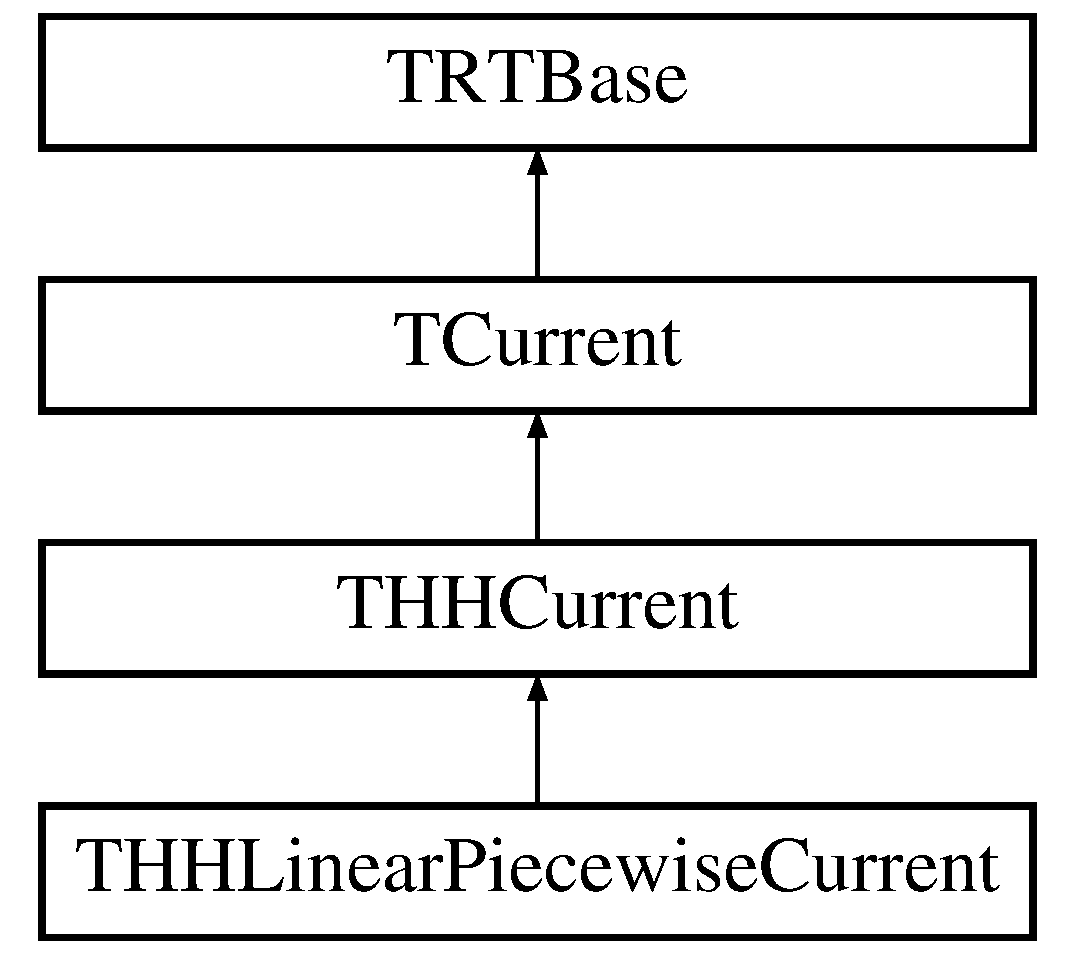
\includegraphics[height=4.000000cm]{class_t_h_h_current}
\end{center}
\end{figure}
\subsection*{Public Member Functions}
\begin{DoxyCompactItemize}
\item 
\hypertarget{class_t_h_h_current_adf34934076fdc9dbe0c2287252e6cd2b}{virtual \hyperlink{class_t_h_h_kinetics_factor}{T\+H\+H\+Kinetics\+Factor} \\*
\&\+\_\+\+\_\+fastcall \hyperlink{class_t_h_h_current_adf34934076fdc9dbe0c2287252e6cd2b}{get\+\_\+m} ()}\label{class_t_h_h_current_adf34934076fdc9dbe0c2287252e6cd2b}

\begin{DoxyCompactList}\small\item\em activation kinetic factor \end{DoxyCompactList}\item 
\hypertarget{class_t_h_h_current_a6c6da3155ae563da18380ad889349187}{virtual \hyperlink{class_t_h_h_kinetics_factor}{T\+H\+H\+Kinetics\+Factor} \\*
\&\+\_\+\+\_\+fastcall \hyperlink{class_t_h_h_current_a6c6da3155ae563da18380ad889349187}{get\+\_\+h} ()}\label{class_t_h_h_current_a6c6da3155ae563da18380ad889349187}

\begin{DoxyCompactList}\small\item\em inactivation kinetic factor \end{DoxyCompactList}\item 
\hypertarget{class_t_h_h_current_a122eaf91312c4bc026f22ed3b29d3ff5}{virtual \hyperlink{class_t_h_h_kinetics_factor}{T\+H\+H\+Kinetics\+Factor} \\*
\&\+\_\+\+\_\+fastcall \hyperlink{class_t_h_h_current_a122eaf91312c4bc026f22ed3b29d3ff5}{get\+\_\+n} ()}\label{class_t_h_h_current_a122eaf91312c4bc026f22ed3b29d3ff5}

\begin{DoxyCompactList}\small\item\em third kinetic factor \end{DoxyCompactList}\item 
bool \+\_\+\+\_\+fastcall \hyperlink{class_t_h_h_current_a4a20db9ff660cafb7d7d05399315f530}{Initialize} (bool Reset)
\begin{DoxyCompactList}\small\item\em Sets Elapsed\+Time to zero. Must be called before first Update. \end{DoxyCompactList}\item 
\hypertarget{class_t_h_h_current_ad754d597753a86b26512ccda217a6790}{bool \+\_\+\+\_\+fastcall \hyperlink{class_t_h_h_current_ad754d597753a86b26512ccda217a6790}{Restart} (double V)}\label{class_t_h_h_current_ad754d597753a86b26512ccda217a6790}

\begin{DoxyCompactList}\small\item\em Initializes kinetic parameters m, h, and n. \end{DoxyCompactList}\item 
const std\+::wstring \&\+\_\+\+\_\+fastcall \hyperlink{class_t_h_h_current_a49049acfa420622d26011f881c432329}{Class\+Key} () const 
\begin{DoxyCompactList}\small\item\em Returns string used to register class with factory. \end{DoxyCompactList}\item 
const void \+\_\+\+\_\+fastcall \hyperlink{class_t_h_h_current_aff79f9a9aa07c2496fcabe97f2ce04a9}{Get\+Param\+Log\+Header} (std\+::vector$<$ std\+::string $>$ \&params) const 
\begin{DoxyCompactList}\small\item\em Supplies column names for parameter logging. \end{DoxyCompactList}\item 
virtual double \+\_\+\+\_\+fastcall \hyperlink{class_t_h_h_current_acaa8176752a6ccc45611d0c80b1a971a}{Do\+Update} (double step, double Vkin, double Vdrv, std\+::vector$<$ double $>$ \&params)
\begin{DoxyCompactList}\small\item\em Calculation of H\+H type current based on two voltages. \end{DoxyCompactList}\item 
\hypertarget{class_t_h_h_current_a6ca4ed77afc56eef5e3bd9ac72c15591}{virtual void \+\_\+\+\_\+fastcall \hyperlink{class_t_h_h_current_a6ca4ed77afc56eef5e3bd9ac72c15591}{Populate\+Edit\+Form} ()}\label{class_t_h_h_current_a6ca4ed77afc56eef5e3bd9ac72c15591}

\begin{DoxyCompactList}\small\item\em Called by G\+U\+I to synchronize edit form with current values of object params. \end{DoxyCompactList}\item 
\hypertarget{class_t_h_h_current_ad147e9579b018f50a6c4244b21e4d105}{virtual bool \+\_\+\+\_\+fastcall \hyperlink{class_t_h_h_current_ad147e9579b018f50a6c4244b21e4d105}{Validate\+Edit\+Form} ()}\label{class_t_h_h_current_ad147e9579b018f50a6c4244b21e4d105}

\begin{DoxyCompactList}\small\item\em Called by G\+U\+I to check if changed values are satisfactory. \end{DoxyCompactList}\item 
\hypertarget{class_t_h_h_current_a3529515fbe5fbcce14fedca3a8db5e04}{virtual void $\ast$const \+\_\+\+\_\+fastcall \hyperlink{class_t_h_h_current_a3529515fbe5fbcce14fedca3a8db5e04}{Get\+Edit\+Form} ()}\label{class_t_h_h_current_a3529515fbe5fbcce14fedca3a8db5e04}

\begin{DoxyCompactList}\small\item\em Returns downcasted T\+H\+H\+Current\+Form$\ast$ that is used to set values for this object. \end{DoxyCompactList}\item 
\hypertarget{class_t_h_h_current_a1cd5d04dc2985d3bd776dbb9e8ed2932}{\+\_\+\+\_\+fastcall \hyperlink{class_t_h_h_current_a1cd5d04dc2985d3bd776dbb9e8ed2932}{T\+H\+H\+Current} ()}\label{class_t_h_h_current_a1cd5d04dc2985d3bd776dbb9e8ed2932}

\begin{DoxyCompactList}\small\item\em default constructor \end{DoxyCompactList}\item 
\hypertarget{class_t_h_h_current_ab1a469b9b65c3a216e956e9542316155}{\+\_\+\+\_\+fastcall \hyperlink{class_t_h_h_current_ab1a469b9b65c3a216e956e9542316155}{T\+H\+H\+Current} (\hyperlink{class_t_current_user}{T\+Current\+User} $\ast$owner, const std\+::wstring \&name)}\label{class_t_h_h_current_ab1a469b9b65c3a216e956e9542316155}

\begin{DoxyCompactList}\small\item\em specialized constructor 2 param \end{DoxyCompactList}\item 
\hypertarget{class_t_h_h_current_a4c14313ed75ec844fbe5c698b1a77d80}{\+\_\+\+\_\+fastcall \hyperlink{class_t_h_h_current_a4c14313ed75ec844fbe5c698b1a77d80}{T\+H\+H\+Current} (const std\+::wstring \&name)}\label{class_t_h_h_current_a4c14313ed75ec844fbe5c698b1a77d80}

\begin{DoxyCompactList}\small\item\em specialized constructor 1 param \end{DoxyCompactList}\item 
\hypertarget{class_t_h_h_current_a43226ed1bcb9c446ecdc8f33365d30e3}{\+\_\+\+\_\+fastcall \hyperlink{class_t_h_h_current_a43226ed1bcb9c446ecdc8f33365d30e3}{T\+H\+H\+Current} (const \hyperlink{class_t_h_h_current}{T\+H\+H\+Current} \&source)}\label{class_t_h_h_current_a43226ed1bcb9c446ecdc8f33365d30e3}

\begin{DoxyCompactList}\small\item\em copy constructor \end{DoxyCompactList}\item 
\hypertarget{class_t_h_h_current_a3b0d3078cf8fddc9b4454eeb8a501a68}{\hyperlink{class_t_h_h_current}{T\+H\+H\+Current} \& \hyperlink{class_t_h_h_current_a3b0d3078cf8fddc9b4454eeb8a501a68}{operator=} (const \hyperlink{class_t_h_h_current}{T\+H\+H\+Current} \&source)}\label{class_t_h_h_current_a3b0d3078cf8fddc9b4454eeb8a501a68}

\begin{DoxyCompactList}\small\item\em overloaded assignment operator \end{DoxyCompactList}\item 
\hypertarget{class_t_h_h_current_a3461a18c4cce4cfc3108791184bf7d3e}{virtual void \+\_\+\+\_\+fastcall \hyperlink{class_t_h_h_current_a3461a18c4cce4cfc3108791184bf7d3e}{Copy\+Params\+From} (const \hyperlink{class_t_current}{T\+Current} $\ast$const source)}\label{class_t_h_h_current_a3461a18c4cce4cfc3108791184bf7d3e}

\begin{DoxyCompactList}\small\item\em overloaded method for duplicating currents without complete assignment \end{DoxyCompactList}\end{DoxyCompactItemize}
\subsection*{Public Attributes}
\begin{DoxyCompactItemize}
\item 
\hypertarget{class_t_h_h_current_aa73d944f399e4c9c35d593a90cae5c69}{\+\_\+\+\_\+property double \hyperlink{class_t_h_h_current_aa73d944f399e4c9c35d593a90cae5c69}{p} = \{read = F\+\_\+p, write = F\+\_\+p\}}\label{class_t_h_h_current_aa73d944f399e4c9c35d593a90cae5c69}

\begin{DoxyCompactList}\small\item\em activation exponent \end{DoxyCompactList}\item 
\hypertarget{class_t_h_h_current_a0b37f38ef5846ae777ae355c4ff9fd58}{\+\_\+\+\_\+property double \hyperlink{class_t_h_h_current_a0b37f38ef5846ae777ae355c4ff9fd58}{q} = \{read = F\+\_\+q, write = F\+\_\+q\}}\label{class_t_h_h_current_a0b37f38ef5846ae777ae355c4ff9fd58}

\begin{DoxyCompactList}\small\item\em inactivation exponent \end{DoxyCompactList}\item 
\hypertarget{class_t_h_h_current_aeb92787a6cc1f7704db0731810f2b3ec}{\+\_\+\+\_\+property double \hyperlink{class_t_h_h_current_aeb92787a6cc1f7704db0731810f2b3ec}{r} = \{read = F\+\_\+r, write = F\+\_\+r\}}\label{class_t_h_h_current_aeb92787a6cc1f7704db0731810f2b3ec}

\begin{DoxyCompactList}\small\item\em third param exponent \end{DoxyCompactList}\item 
\hypertarget{class_t_h_h_current_a1396d7860bf5838e11577389ff9dcd09}{\+\_\+\+\_\+property double \hyperlink{class_t_h_h_current_a1396d7860bf5838e11577389ff9dcd09}{E} = \{read = F\+\_\+\+E, write = F\+\_\+\+E\}}\label{class_t_h_h_current_a1396d7860bf5838e11577389ff9dcd09}

\begin{DoxyCompactList}\small\item\em reversal potential (m\+V) \end{DoxyCompactList}\item 
\hypertarget{class_t_h_h_current_a78154399d225a791f4dfd93546de6903}{\+\_\+\+\_\+property double \hyperlink{class_t_h_h_current_a78154399d225a791f4dfd93546de6903}{Gmax} = \{read = F\+\_\+\+Gmax, write = F\+\_\+\+Gmax\}}\label{class_t_h_h_current_a78154399d225a791f4dfd93546de6903}

\begin{DoxyCompactList}\small\item\em mean maximum conductance (u\+S) \end{DoxyCompactList}\item 
\hypertarget{class_t_h_h_current_a62dbf34311e4c433d6bcfda9497982f9}{\+\_\+\+\_\+property double \hyperlink{class_t_h_h_current_a62dbf34311e4c433d6bcfda9497982f9}{Gnoise} = \{read = F\+\_\+\+Gnoise, write = F\+\_\+\+Gnoise\}}\label{class_t_h_h_current_a62dbf34311e4c433d6bcfda9497982f9}

\begin{DoxyCompactList}\small\item\em Variation about mean conductance (\%) \end{DoxyCompactList}\end{DoxyCompactItemize}
\subsection*{Protected Member Functions}
\begin{DoxyCompactItemize}
\item 
\hypertarget{class_t_h_h_current_a28afc4ddd30bbf6a44855c750a98dc8d}{virtual void const \+\_\+\+\_\+fastcall \hyperlink{class_t_h_h_current_a28afc4ddd30bbf6a44855c750a98dc8d}{Write\+To\+Stream} (ostream \&stream) const }\label{class_t_h_h_current_a28afc4ddd30bbf6a44855c750a98dc8d}

\begin{DoxyCompactList}\small\item\em Writes data members to a stream. \end{DoxyCompactList}\item 
\hypertarget{class_t_h_h_current_a9ade3361c30cf11880d13339f7ae1fad}{virtual void const \+\_\+\+\_\+fastcall \hyperlink{class_t_h_h_current_a9ade3361c30cf11880d13339f7ae1fad}{Read\+From\+Stream} (istream \&stream)}\label{class_t_h_h_current_a9ade3361c30cf11880d13339f7ae1fad}

\begin{DoxyCompactList}\small\item\em Reads data members from a stream. \end{DoxyCompactList}\end{DoxyCompactItemize}
\subsection*{Protected Attributes}
\begin{DoxyCompactItemize}
\item 
\hypertarget{class_t_h_h_current_a8938eaa4d33700d8b2de8a2b7ef918e9}{long {\bfseries idum}}\label{class_t_h_h_current_a8938eaa4d33700d8b2de8a2b7ef918e9}

\end{DoxyCompactItemize}
\subsection*{Friends}
\begin{DoxyCompactItemize}
\item 
\hypertarget{class_t_h_h_current_ac98d07dd8f7b70e16ccb9a01abf56b9c}{class {\bfseries boost\+::serialization\+::access}}\label{class_t_h_h_current_ac98d07dd8f7b70e16ccb9a01abf56b9c}

\end{DoxyCompactItemize}


\subsection{Detailed Description}
Implementation of Hodgkin-\/\+Huxley type current with Tohidi-\/\+Nadim shortcuts. 


\begin{DoxyPre}
 Classes \hyperlink{class_t_h_h_current}{THHCurrent} gives ionic current as a function of several kinetic
 parameters and the input voltages V\_kin and V\_drv.  For intrinsic currents
 V\_drv = V\_kin, and for synaptic currents, V\_kin is the voltage of the
 presynaptic cell.\end{DoxyPre}



\begin{DoxyPre}                      p   q   r
 computes I = Gmax * m * h * n * (V\_drv - E)
\end{DoxyPre}


\begin{DoxyAuthor}{Author}
E. Brady Trexler $<$ebtrexler (at) gothamsci.\+com$>$, 2011 -\/ 2013 
\end{DoxyAuthor}


\subsection{Member Function Documentation}
\hypertarget{class_t_h_h_current_a49049acfa420622d26011f881c432329}{\index{T\+H\+H\+Current@{T\+H\+H\+Current}!Class\+Key@{Class\+Key}}
\index{Class\+Key@{Class\+Key}!T\+H\+H\+Current@{T\+H\+H\+Current}}
\subsubsection[{Class\+Key}]{\setlength{\rightskip}{0pt plus 5cm}const std\+::wstring \&\+\_\+\+\_\+fastcall T\+H\+H\+Current\+::\+Class\+Key (
\begin{DoxyParamCaption}
{}
\end{DoxyParamCaption}
) const\hspace{0.3cm}{\ttfamily [virtual]}}}\label{class_t_h_h_current_a49049acfa420622d26011f881c432329}


Returns string used to register class with factory. 

Users of class factories must also tell the class the key they used when registering the class. See factory.\+h 

Implements \hyperlink{class_t_r_t_base_a6083fd510cbcb00faa85e5934fc3c18e}{T\+R\+T\+Base}.



Reimplemented in \hyperlink{class_t_h_h_linear_piecewise_current_a2f62f65488ad9489bdf671b6fd4dd837}{T\+H\+H\+Linear\+Piecewise\+Current}.

\hypertarget{class_t_h_h_current_acaa8176752a6ccc45611d0c80b1a971a}{\index{T\+H\+H\+Current@{T\+H\+H\+Current}!Do\+Update@{Do\+Update}}
\index{Do\+Update@{Do\+Update}!T\+H\+H\+Current@{T\+H\+H\+Current}}
\subsubsection[{Do\+Update}]{\setlength{\rightskip}{0pt plus 5cm}double \+\_\+\+\_\+fastcall T\+H\+H\+Current\+::\+Do\+Update (
\begin{DoxyParamCaption}
\item[{double}]{step, }
\item[{double}]{Vkin, }
\item[{double}]{Vdrv, }
\item[{std\+::vector$<$ double $>$ \&}]{params}
\end{DoxyParamCaption}
)\hspace{0.3cm}{\ttfamily [virtual]}}}\label{class_t_h_h_current_acaa8176752a6ccc45611d0c80b1a971a}


Calculation of H\+H type current based on two voltages. 


\begin{DoxyPre}
                                     p         q         r
          computes I = Gmax * m(Vkin) * h(Vkin) * n(Vkin) * (Vdrv - E)
\end{DoxyPre}
 

Implements \hyperlink{class_t_current_a36d89025eb424f6905fef945c9ae4fa7}{T\+Current}.



Reimplemented in \hyperlink{class_t_h_h_linear_piecewise_current_a7607b43e63ba9761d083aba7c25edfd6}{T\+H\+H\+Linear\+Piecewise\+Current}.

\hypertarget{class_t_h_h_current_aff79f9a9aa07c2496fcabe97f2ce04a9}{\index{T\+H\+H\+Current@{T\+H\+H\+Current}!Get\+Param\+Log\+Header@{Get\+Param\+Log\+Header}}
\index{Get\+Param\+Log\+Header@{Get\+Param\+Log\+Header}!T\+H\+H\+Current@{T\+H\+H\+Current}}
\subsubsection[{Get\+Param\+Log\+Header}]{\setlength{\rightskip}{0pt plus 5cm}const void \+\_\+\+\_\+fastcall T\+H\+H\+Current\+::\+Get\+Param\+Log\+Header (
\begin{DoxyParamCaption}
\item[{std\+::vector$<$ std\+::string $>$ \&}]{params}
\end{DoxyParamCaption}
) const\hspace{0.3cm}{\ttfamily [virtual]}}}\label{class_t_h_h_current_aff79f9a9aa07c2496fcabe97f2ce04a9}


Supplies column names for parameter logging. 


\begin{DoxyParams}{Parameters}
{\em params} & = vector of parameter names for logging Override in derived classes to add their parameters to the header \\
\hline
\end{DoxyParams}


Implements \hyperlink{class_t_current_ab49cb51723efade5eec00fa78fad7ad8}{T\+Current}.

\hypertarget{class_t_h_h_current_a4a20db9ff660cafb7d7d05399315f530}{\index{T\+H\+H\+Current@{T\+H\+H\+Current}!Initialize@{Initialize}}
\index{Initialize@{Initialize}!T\+H\+H\+Current@{T\+H\+H\+Current}}
\subsubsection[{Initialize}]{\setlength{\rightskip}{0pt plus 5cm}bool \+\_\+\+\_\+fastcall T\+H\+H\+Current\+::\+Initialize (
\begin{DoxyParamCaption}
\item[{bool}]{reset}
\end{DoxyParamCaption}
)\hspace{0.3cm}{\ttfamily [virtual]}}}\label{class_t_h_h_current_a4a20db9ff660cafb7d7d05399315f530}


Sets Elapsed\+Time to zero. Must be called before first Update. 


\begin{DoxyParams}{Parameters}
{\em reset} & = flag for derived classes \\
\hline
\end{DoxyParams}


Reimplemented from \hyperlink{class_t_current_a00c70d232ae85a9841d8d07e5770b7bd}{T\+Current}.



The documentation for this class was generated from the following files\+:\begin{DoxyCompactItemize}
\item 
R\+T\+\_\+\+H\+H\+Current.\+h\item 
R\+T\+\_\+\+H\+H\+Current.\+cpp\end{DoxyCompactItemize}

\hypertarget{class_t_h_h_current_form}{\section{T\+H\+H\+Current\+Form Class Reference}
\label{class_t_h_h_current_form}\index{T\+H\+H\+Current\+Form@{T\+H\+H\+Current\+Form}}
}


G\+U\+I editor for \hyperlink{class_t_h_h_current}{T\+H\+H\+Current}.  




{\ttfamily \#include $<$G\+U\+I\+\_\+\+R\+T\+\_\+\+Edit\+\_\+\+H\+H\+Current.\+h$>$}

Inheritance diagram for T\+H\+H\+Current\+Form\+:\begin{figure}[H]
\begin{center}
\leavevmode
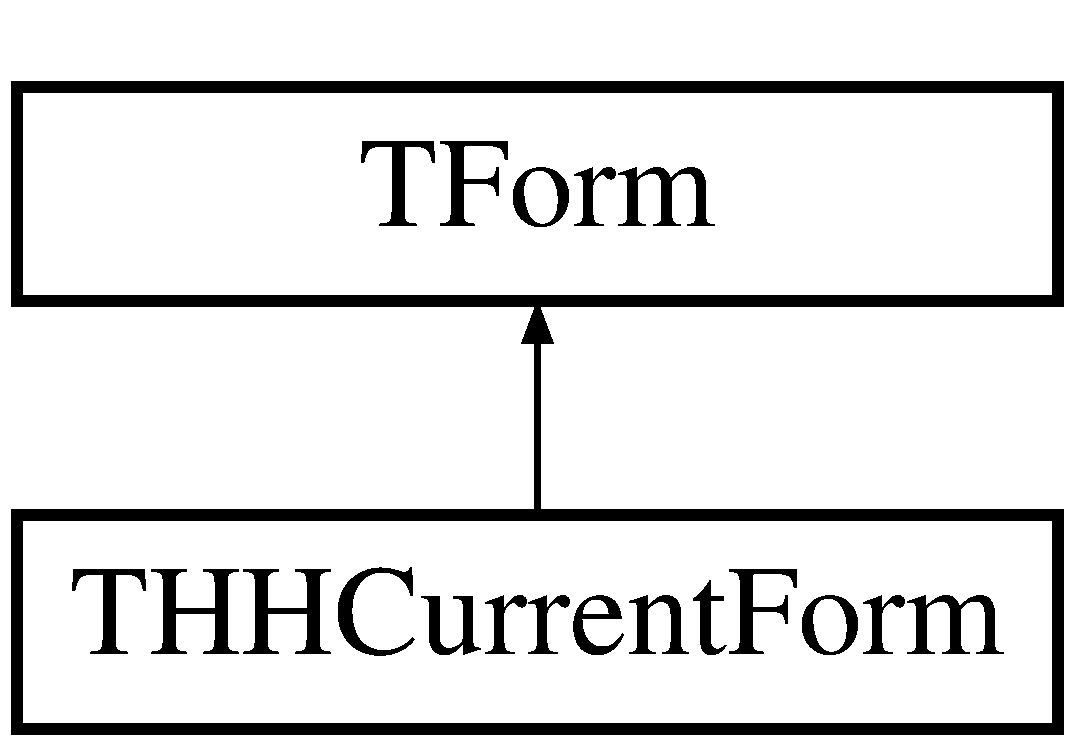
\includegraphics[height=2.000000cm]{class_t_h_h_current_form}
\end{center}
\end{figure}
\subsection*{Public Member Functions}
\begin{DoxyCompactItemize}
\item 
\hypertarget{class_t_h_h_current_form_a1e5dcab20fa6d9eae39835085ac923f0}{void \+\_\+\+\_\+fastcall \hyperlink{class_t_h_h_current_form_a1e5dcab20fa6d9eae39835085ac923f0}{Params\+Editors\+\_\+\+Key\+Press} (T\+Object $\ast$Sender, wchar\+\_\+t \&Key)}\label{class_t_h_h_current_form_a1e5dcab20fa6d9eae39835085ac923f0}

\begin{DoxyCompactList}\small\item\em Calls Update\+Plots to reflect changes if valid, otherwise no changes accepted. \end{DoxyCompactList}\item 
\hypertarget{class_t_h_h_current_form_a7c2279508a7f4d1eb1c2a73c64f75acf}{void \+\_\+\+\_\+fastcall \hyperlink{class_t_h_h_current_form_a7c2279508a7f4d1eb1c2a73c64f75acf}{Load\+Button\+Click} (T\+Object $\ast$Sender)}\label{class_t_h_h_current_form_a7c2279508a7f4d1eb1c2a73c64f75acf}

\begin{DoxyCompactList}\small\item\em Opens saved parameters from dialog-\/chosen file. \end{DoxyCompactList}\item 
\hypertarget{class_t_h_h_current_form_a0e30e6f1106039c94115d0e8b1b8add8}{void \+\_\+\+\_\+fastcall \hyperlink{class_t_h_h_current_form_a0e30e6f1106039c94115d0e8b1b8add8}{Save\+Button\+Click} (T\+Object $\ast$Sender)}\label{class_t_h_h_current_form_a0e30e6f1106039c94115d0e8b1b8add8}

\begin{DoxyCompactList}\small\item\em Saves parameters to dialog-\/chosen file. \end{DoxyCompactList}\item 
\hypertarget{class_t_h_h_current_form_a48809e8ad50543c9e2e293eea6847039}{void \+\_\+\+\_\+fastcall {\bfseries Period\+Edit\+Button\+Click} (T\+Object $\ast$Sender)}\label{class_t_h_h_current_form_a48809e8ad50543c9e2e293eea6847039}

\item 
\hypertarget{class_t_h_h_current_form_a0d9286e27a4db14216faac7ce1f802a2}{void \+\_\+\+\_\+fastcall {\bfseries Use\+Vdrv\+Combo\+Box\+Click} (T\+Object $\ast$Sender)}\label{class_t_h_h_current_form_a0d9286e27a4db14216faac7ce1f802a2}

\item 
\hypertarget{class_t_h_h_current_form_a61b7d438d75f3d595483dc19c11f1a7b}{void \+\_\+\+\_\+fastcall \hyperlink{class_t_h_h_current_form_a61b7d438d75f3d595483dc19c11f1a7b}{Update\+Plots} ()}\label{class_t_h_h_current_form_a61b7d438d75f3d595483dc19c11f1a7b}

\begin{DoxyCompactList}\small\item\em Called when parameter changes need to be reflected in G\+U\+I. \end{DoxyCompactList}\item 
\hypertarget{class_t_h_h_current_form_a31b1200632d593492821cb2f54ce2319}{\+\_\+\+\_\+fastcall \hyperlink{class_t_h_h_current_form_a31b1200632d593492821cb2f54ce2319}{T\+H\+H\+Current\+Form} (T\+Component $\ast$Owner)}\label{class_t_h_h_current_form_a31b1200632d593492821cb2f54ce2319}

\begin{DoxyCompactList}\small\item\em Constructor that builds the form and plots to show params. \end{DoxyCompactList}\end{DoxyCompactItemize}
\subsection*{Public Attributes}
\begin{DoxyCompactItemize}
\item 
\hypertarget{class_t_h_h_current_form_a0fac9b873a7f2d422542f6a7ec7d74d4}{T\+Group\+Box $\ast$ {\bfseries Group\+Box1}}\label{class_t_h_h_current_form_a0fac9b873a7f2d422542f6a7ec7d74d4}

\item 
\hypertarget{class_t_h_h_current_form_aafb019a81b2e9d56fb5b424ab5fdf51e}{T\+Panel $\ast$ {\bfseries Panel1}}\label{class_t_h_h_current_form_aafb019a81b2e9d56fb5b424ab5fdf51e}

\item 
\hypertarget{class_t_h_h_current_form_ab61f0a096aae196111b0923a65a152af}{T\+Value\+List\+Editor $\ast$ {\bfseries Value\+List\+Editor\+\_\+m}}\label{class_t_h_h_current_form_ab61f0a096aae196111b0923a65a152af}

\item 
\hypertarget{class_t_h_h_current_form_ad63b6047704a7c4dec3bf02ef9a83513}{T\+Group\+Box $\ast$ {\bfseries Group\+Box2}}\label{class_t_h_h_current_form_ad63b6047704a7c4dec3bf02ef9a83513}

\item 
\hypertarget{class_t_h_h_current_form_afed927065064065b3178138763fccbe7}{T\+Panel $\ast$ {\bfseries Panel2}}\label{class_t_h_h_current_form_afed927065064065b3178138763fccbe7}

\item 
\hypertarget{class_t_h_h_current_form_a16ca77686ef30a6925b6313b3539411c}{T\+Value\+List\+Editor $\ast$ {\bfseries Value\+List\+Editor\+\_\+h}}\label{class_t_h_h_current_form_a16ca77686ef30a6925b6313b3539411c}

\item 
\hypertarget{class_t_h_h_current_form_a53d70c024e556d69c0bc61f4e63c7e3c}{T\+Label $\ast$ {\bfseries Label1}}\label{class_t_h_h_current_form_a53d70c024e556d69c0bc61f4e63c7e3c}

\item 
\hypertarget{class_t_h_h_current_form_a4f6ba8133879ea576f10cb75413a7d6d}{T\+Label $\ast$ {\bfseries Label2}}\label{class_t_h_h_current_form_a4f6ba8133879ea576f10cb75413a7d6d}

\item 
\hypertarget{class_t_h_h_current_form_aefb08748e9aab83dcb112f3e85b9bc45}{T\+Label $\ast$ {\bfseries Label3}}\label{class_t_h_h_current_form_aefb08748e9aab83dcb112f3e85b9bc45}

\item 
\hypertarget{class_t_h_h_current_form_ad3334edeae3b46c92de618c24c4da9d8}{T\+Label $\ast$ {\bfseries Label4}}\label{class_t_h_h_current_form_ad3334edeae3b46c92de618c24c4da9d8}

\item 
\hypertarget{class_t_h_h_current_form_a071ede513908ac6935e9466f92d20b03}{T\+Edit $\ast$ {\bfseries Gmax\+Edit}}\label{class_t_h_h_current_form_a071ede513908ac6935e9466f92d20b03}

\item 
\hypertarget{class_t_h_h_current_form_a0973e083bbebcd51f499ad00f67b8437}{T\+Edit $\ast$ {\bfseries Erev\+Edit}}\label{class_t_h_h_current_form_a0973e083bbebcd51f499ad00f67b8437}

\item 
\hypertarget{class_t_h_h_current_form_a8b02654ca9924a9a675eb754c83a096b}{T\+Button $\ast$ {\bfseries Load\+Button}}\label{class_t_h_h_current_form_a8b02654ca9924a9a675eb754c83a096b}

\item 
\hypertarget{class_t_h_h_current_form_ae85631cd95fd13f51fc8860714fbcdbd}{T\+Button $\ast$ {\bfseries Save\+Button}}\label{class_t_h_h_current_form_ae85631cd95fd13f51fc8860714fbcdbd}

\item 
\hypertarget{class_t_h_h_current_form_a89c3c40ff820afc1e516f3ce3d60081e}{T\+Multi\+P\+L\+O\+T\+Panel $\ast$ {\bfseries Multi\+Plot\+Panel1}}\label{class_t_h_h_current_form_a89c3c40ff820afc1e516f3ce3d60081e}

\item 
\hypertarget{class_t_h_h_current_form_a9912b46c5293eb9b510aa971e2b87c37}{T\+Group\+Box $\ast$ {\bfseries Group\+Box3}}\label{class_t_h_h_current_form_a9912b46c5293eb9b510aa971e2b87c37}

\item 
\hypertarget{class_t_h_h_current_form_ae465c1f90d7a2cd783a75bafc2a2dc06}{T\+Panel $\ast$ {\bfseries Panel3}}\label{class_t_h_h_current_form_ae465c1f90d7a2cd783a75bafc2a2dc06}

\item 
\hypertarget{class_t_h_h_current_form_a7248ff3ce29f6c1c913fb0f1dcca1d91}{T\+Value\+List\+Editor $\ast$ {\bfseries Value\+List\+Editor\+\_\+n}}\label{class_t_h_h_current_form_a7248ff3ce29f6c1c913fb0f1dcca1d91}

\item 
\hypertarget{class_t_h_h_current_form_abda67e306fc2e67a53dbe973a6f30434}{T\+Label $\ast$ {\bfseries Label5}}\label{class_t_h_h_current_form_abda67e306fc2e67a53dbe973a6f30434}

\item 
\hypertarget{class_t_h_h_current_form_a3fca443996bd126729ce97915bc7dab5}{T\+Open\+Dialog $\ast$ {\bfseries Open\+Dialog1}}\label{class_t_h_h_current_form_a3fca443996bd126729ce97915bc7dab5}

\item 
\hypertarget{class_t_h_h_current_form_a1899940a9ba40db57037327f0d915ed3}{T\+Save\+Dialog $\ast$ {\bfseries Save\+Dialog1}}\label{class_t_h_h_current_form_a1899940a9ba40db57037327f0d915ed3}

\item 
\hypertarget{class_t_h_h_current_form_a132a094e6bfd5f826b8a21f2a1236350}{T\+Edit $\ast$ {\bfseries Gnoise\+Edit}}\label{class_t_h_h_current_form_a132a094e6bfd5f826b8a21f2a1236350}

\item 
\hypertarget{class_t_h_h_current_form_aebf894ced65af134059c44a33d26e868}{T\+Label $\ast$ {\bfseries Label6}}\label{class_t_h_h_current_form_aebf894ced65af134059c44a33d26e868}

\item 
\hypertarget{class_t_h_h_current_form_a8185f33a7a92532e0f94c4625c4e8628}{T\+Label $\ast$ {\bfseries Label7}}\label{class_t_h_h_current_form_a8185f33a7a92532e0f94c4625c4e8628}

\item 
\hypertarget{class_t_h_h_current_form_aa163f4faacd1911131d8fe82af3b79fe}{T\+Label $\ast$ {\bfseries Label8}}\label{class_t_h_h_current_form_aa163f4faacd1911131d8fe82af3b79fe}

\item 
\hypertarget{class_t_h_h_current_form_a40dab153d652b604ec1e14b6f3af9d87}{T\+Panel $\ast$ {\bfseries Panel4}}\label{class_t_h_h_current_form_a40dab153d652b604ec1e14b6f3af9d87}

\item 
\hypertarget{class_t_h_h_current_form_abb8f6d907bd5e49ab8fbf947f271d019}{T\+Panel $\ast$ {\bfseries Panel5}}\label{class_t_h_h_current_form_abb8f6d907bd5e49ab8fbf947f271d019}

\item 
\hypertarget{class_t_h_h_current_form_a24cb0157bc839283cad35c52a4ad8ab7}{T\+Check\+Box $\ast$ {\bfseries Periodic\+Check\+Box}}\label{class_t_h_h_current_form_a24cb0157bc839283cad35c52a4ad8ab7}

\item 
\hypertarget{class_t_h_h_current_form_a1825c671bc80ee3884d7c0dc39904439}{T\+Button $\ast$ {\bfseries Period\+Edit\+Button}}\label{class_t_h_h_current_form_a1825c671bc80ee3884d7c0dc39904439}

\item 
\hypertarget{class_t_h_h_current_form_ad04fb7167ed1511fc086374125492ff9}{T\+Check\+Box $\ast$ {\bfseries Param\+Logging\+Check\+Box}}\label{class_t_h_h_current_form_ad04fb7167ed1511fc086374125492ff9}

\item 
\hypertarget{class_t_h_h_current_form_a87de73b8f08a686e0b18be094ebac998}{T\+Panel $\ast$ {\bfseries Panel6}}\label{class_t_h_h_current_form_a87de73b8f08a686e0b18be094ebac998}

\item 
\hypertarget{class_t_h_h_current_form_a17a84cf0c50393eb2d4cc4b3438c8e67}{T\+Check\+Box $\ast$ {\bfseries Use\+Vdrv\+Combo\+Box}}\label{class_t_h_h_current_form_a17a84cf0c50393eb2d4cc4b3438c8e67}

\item 
\hypertarget{class_t_h_h_current_form_a06eda24da690235897f1c8d933b82d8d}{\hyperlink{class_t_h_h_current}{T\+H\+H\+Current} $\ast$ {\bfseries H\+H\+Current}}\label{class_t_h_h_current_form_a06eda24da690235897f1c8d933b82d8d}

\item 
\hypertarget{class_t_h_h_current_form_a39b4101723007a93a5fc6ccae510eab2}{\hyperlink{class_t_periodicity_form}{T\+Periodicity\+Form} $\ast$ {\bfseries Current\+Period\+Form}}\label{class_t_h_h_current_form_a39b4101723007a93a5fc6ccae510eab2}

\end{DoxyCompactItemize}


\subsection{Detailed Description}
G\+U\+I editor for \hyperlink{class_t_h_h_current}{T\+H\+H\+Current}. 

\begin{DoxyAuthor}{Author}
E. Brady Trexler $<$ebtrexler (at) gothamsci.\+com$>$, 2011 -\/ 2013 
\end{DoxyAuthor}


The documentation for this class was generated from the following files\+:\begin{DoxyCompactItemize}
\item 
G\+U\+I\+\_\+\+R\+T\+\_\+\+Edit\+\_\+\+H\+H\+Current.\+h\item 
G\+U\+I\+\_\+\+R\+T\+\_\+\+Edit\+\_\+\+H\+H\+Current.\+cpp\end{DoxyCompactItemize}

\hypertarget{class_t_h_h_current_model}{\section{T\+H\+H\+Current\+Model Class Reference}
\label{class_t_h_h_current_model}\index{T\+H\+H\+Current\+Model@{T\+H\+H\+Current\+Model}}
}
Inheritance diagram for T\+H\+H\+Current\+Model\+:\begin{figure}[H]
\begin{center}
\leavevmode
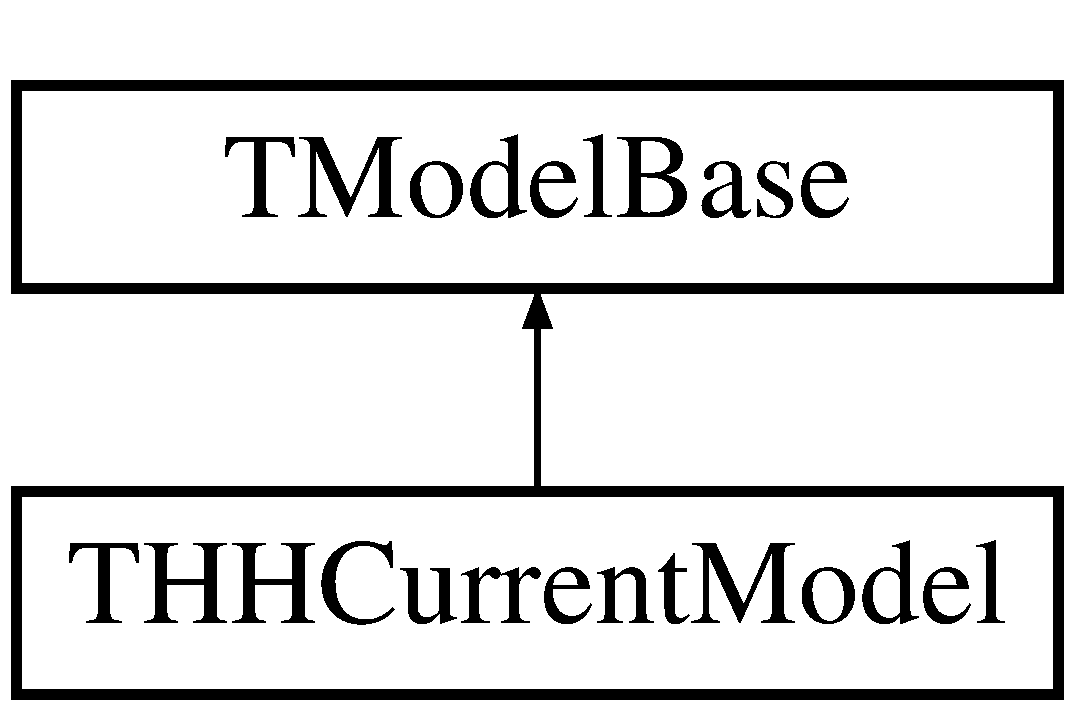
\includegraphics[height=2.000000cm]{class_t_h_h_current_model}
\end{center}
\end{figure}
\subsection*{Public Member Functions}
\begin{DoxyCompactItemize}
\item 
\hypertarget{class_t_h_h_current_model_ae198bcc354862e2cf7b0094da7288ec2}{virtual int \+\_\+\+\_\+fastcall {\bfseries Out\+Fit} ()}\label{class_t_h_h_current_model_ae198bcc354862e2cf7b0094da7288ec2}

\item 
\hypertarget{class_t_h_h_current_model_a4f95f6bb4f4fc3c78347f3794b3ab246}{virtual double \+\_\+\+\_\+fastcall {\bfseries Get\+Chi\+Sq} ()}\label{class_t_h_h_current_model_a4f95f6bb4f4fc3c78347f3794b3ab246}

\item 
\hypertarget{class_t_h_h_current_model_ae561975a3f295965ec98cce52a7d90a5}{virtual int \+\_\+\+\_\+fastcall {\bfseries fit\+Gen} (int $\ast$numdatapoints, int $\ast$numparms, double $\ast$parms, double $\ast$fvec, int $\ast$iflag)}\label{class_t_h_h_current_model_ae561975a3f295965ec98cce52a7d90a5}

\item 
\hypertarget{class_t_h_h_current_model_aa0c6d4dd0c86cd1ba2272e43993e452d}{void \+\_\+\+\_\+fastcall {\bfseries Stuff\+Parms} (double $\ast$parms)}\label{class_t_h_h_current_model_aa0c6d4dd0c86cd1ba2272e43993e452d}

\item 
\hypertarget{class_t_h_h_current_model_aeff8b76dd51218f92ce08e22a3956631}{void \+\_\+\+\_\+fastcall {\bfseries Pop\+To\+Fit\+Parms} ()}\label{class_t_h_h_current_model_aeff8b76dd51218f92ce08e22a3956631}

\item 
\hypertarget{class_t_h_h_current_model_a00edf58566894d52aaaadad98d28c075}{void \+\_\+\+\_\+fastcall {\bfseries Setup} (int currchan, int voltchan)}\label{class_t_h_h_current_model_a00edf58566894d52aaaadad98d28c075}

\item 
\hypertarget{class_t_h_h_current_model_add870dba1a7d86a9031f72ed8a7653f1}{int \+\_\+\+\_\+fastcall {\bfseries i\+Gen} (std\+::vector$<$ double $>$ \&to\+Fill)}\label{class_t_h_h_current_model_add870dba1a7d86a9031f72ed8a7653f1}

\end{DoxyCompactItemize}
\subsection*{Public Attributes}
\begin{DoxyCompactItemize}
\item 
\hypertarget{class_t_h_h_current_model_a89f3e258927c21ad4263cec1d42c3893}{\hyperlink{class_t_playback_waveform}{T\+Playback\+Waveform} $\ast$ {\bfseries Waveform}}\label{class_t_h_h_current_model_a89f3e258927c21ad4263cec1d42c3893}

\item 
\hypertarget{class_t_h_h_current_model_a3d3076f6fca670df64cf98c38ae21800}{\hyperlink{class_t_h_h_current}{T\+H\+H\+Current} $\ast$ {\bfseries Current}}\label{class_t_h_h_current_model_a3d3076f6fca670df64cf98c38ae21800}

\item 
\hypertarget{class_t_h_h_current_model_a08b581933f4643976cedbcca848d3f77}{double {\bfseries Sample\+Rate}}\label{class_t_h_h_current_model_a08b581933f4643976cedbcca848d3f77}

\item 
\hypertarget{class_t_h_h_current_model_ac0b430e2c3c82b5e0c9fdaab4390c2b4}{int {\bfseries Num\+Episodes}}\label{class_t_h_h_current_model_ac0b430e2c3c82b5e0c9fdaab4390c2b4}

\item 
\hypertarget{class_t_h_h_current_model_af91a84197199459314301d81926ea5cd}{int {\bfseries Num\+Points\+Per\+Episode}}\label{class_t_h_h_current_model_af91a84197199459314301d81926ea5cd}

\item 
\hypertarget{class_t_h_h_current_model_af97d27e7a3736d5850046fddebd6e934}{std\+::vector$<$ double $>$ {\bfseries voltdata}}\label{class_t_h_h_current_model_af97d27e7a3736d5850046fddebd6e934}

\item 
\hypertarget{class_t_h_h_current_model_a99fdc6e25ff271ff59aee23a82b51739}{std\+::vector$<$ double $>$ {\bfseries currdata}}\label{class_t_h_h_current_model_a99fdc6e25ff271ff59aee23a82b51739}

\item 
\hypertarget{class_t_h_h_current_model_a235d0be2b3ccf7e3d62d8b8335aba535}{std\+::vector$<$ double $>$ {\bfseries fitdata}}\label{class_t_h_h_current_model_a235d0be2b3ccf7e3d62d8b8335aba535}

\end{DoxyCompactItemize}


The documentation for this class was generated from the following files\+:\begin{DoxyCompactItemize}
\item 
Fit\+\_\+\+H\+H\+Current.\+h\item 
Fit\+\_\+\+H\+H\+Current.\+cpp\end{DoxyCompactItemize}

\hypertarget{class_t_h_h_kinetics_factor}{\section{T\+H\+H\+Kinetics\+Factor Class Reference}
\label{class_t_h_h_kinetics_factor}\index{T\+H\+H\+Kinetics\+Factor@{T\+H\+H\+Kinetics\+Factor}}
}


Kinetic factor used by \hyperlink{class_t_h_h_current}{T\+H\+H\+Current}.  




{\ttfamily \#include $<$R\+T\+\_\+\+H\+H\+Kinetics\+Factor.\+h$>$}

Inheritance diagram for T\+H\+H\+Kinetics\+Factor\+:\begin{figure}[H]
\begin{center}
\leavevmode
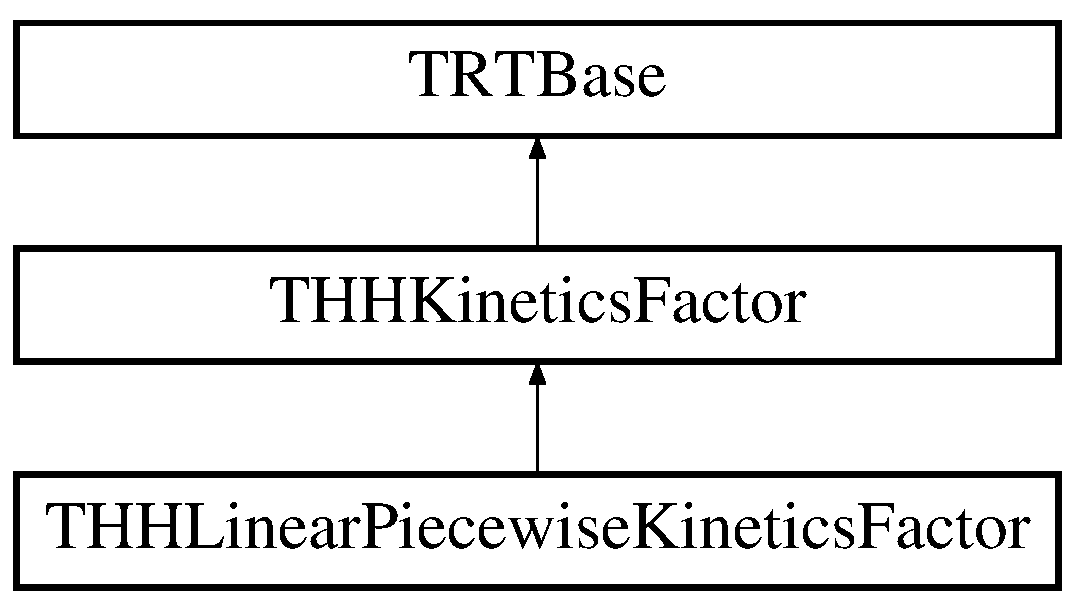
\includegraphics[height=3.000000cm]{class_t_h_h_kinetics_factor}
\end{center}
\end{figure}
\subsection*{Public Member Functions}
\begin{DoxyCompactItemize}
\item 
\hypertarget{class_t_h_h_kinetics_factor_a781fb1bd7d2f85e9193f2f6c4d81d058}{virtual bool \+\_\+\+\_\+fastcall \hyperlink{class_t_h_h_kinetics_factor_a781fb1bd7d2f85e9193f2f6c4d81d058}{Initialize} (bool Reset)}\label{class_t_h_h_kinetics_factor_a781fb1bd7d2f85e9193f2f6c4d81d058}

\begin{DoxyCompactList}\small\item\em Override pure virtual. \end{DoxyCompactList}\item 
\hypertarget{class_t_h_h_kinetics_factor_a587e585d53381e0194c5f98e1f0cb0f6}{virtual bool \+\_\+\+\_\+fastcall \hyperlink{class_t_h_h_kinetics_factor_a587e585d53381e0194c5f98e1f0cb0f6}{Restart} (double V)}\label{class_t_h_h_kinetics_factor_a587e585d53381e0194c5f98e1f0cb0f6}

\begin{DoxyCompactList}\small\item\em Sets variables (tau, inf) to steady state values before new run. \end{DoxyCompactList}\item 
const std\+::wstring \&\+\_\+\+\_\+fastcall \hyperlink{class_t_h_h_kinetics_factor_ac161d432e14597146b0bd45cbed7e225}{Class\+Key} () const 
\begin{DoxyCompactList}\small\item\em Returns string used to register class with factory. \end{DoxyCompactList}\item 
double \+\_\+\+\_\+fastcall \hyperlink{class_t_h_h_kinetics_factor_aa673d6cce19ae2a1e834fa1a99ef4130}{Update} (double V, double step)
\begin{DoxyCompactList}\small\item\em Called by \hyperlink{class_t_h_h_current}{T\+H\+H\+Current} to get new value of kinetic parameter. \end{DoxyCompactList}\item 
\hypertarget{class_t_h_h_kinetics_factor_a52ed711cf78c030d5e8fe7b19fb5a1dc}{virtual double \hyperlink{class_t_h_h_kinetics_factor_a52ed711cf78c030d5e8fe7b19fb5a1dc}{tau} (double V)}\label{class_t_h_h_kinetics_factor_a52ed711cf78c030d5e8fe7b19fb5a1dc}

\begin{DoxyCompactList}\small\item\em Calculates new value of tau from given voltage, V. \end{DoxyCompactList}\item 
\hypertarget{class_t_h_h_kinetics_factor_a21c8dff53e3fd122ac0a59bcc97e4b61}{virtual double \hyperlink{class_t_h_h_kinetics_factor_a21c8dff53e3fd122ac0a59bcc97e4b61}{inf} (double V)}\label{class_t_h_h_kinetics_factor_a21c8dff53e3fd122ac0a59bcc97e4b61}

\begin{DoxyCompactList}\small\item\em Calculates new value of inf from given voltage, V. \end{DoxyCompactList}\item 
\hypertarget{class_t_h_h_kinetics_factor_a2c636c0456e3999dea4079fbc13fd6e6}{\+\_\+\+\_\+fastcall \hyperlink{class_t_h_h_kinetics_factor_a2c636c0456e3999dea4079fbc13fd6e6}{T\+H\+H\+Kinetics\+Factor} ()}\label{class_t_h_h_kinetics_factor_a2c636c0456e3999dea4079fbc13fd6e6}

\begin{DoxyCompactList}\small\item\em default constructor \end{DoxyCompactList}\item 
\hypertarget{class_t_h_h_kinetics_factor_ae08ba4b5b090e47556c5f7e6a461b96a}{\+\_\+\+\_\+fastcall \hyperlink{class_t_h_h_kinetics_factor_ae08ba4b5b090e47556c5f7e6a461b96a}{T\+H\+H\+Kinetics\+Factor} (const \hyperlink{class_t_h_h_kinetics_factor}{T\+H\+H\+Kinetics\+Factor} \&source)}\label{class_t_h_h_kinetics_factor_ae08ba4b5b090e47556c5f7e6a461b96a}

\begin{DoxyCompactList}\small\item\em copy constructor \end{DoxyCompactList}\item 
\hypertarget{class_t_h_h_kinetics_factor_af303980a4fda7ec3868922163a121f26}{\hyperlink{class_t_h_h_kinetics_factor}{T\+H\+H\+Kinetics\+Factor} \& \hyperlink{class_t_h_h_kinetics_factor_af303980a4fda7ec3868922163a121f26}{operator=} (const \hyperlink{class_t_h_h_kinetics_factor}{T\+H\+H\+Kinetics\+Factor} \&source)}\label{class_t_h_h_kinetics_factor_af303980a4fda7ec3868922163a121f26}

\begin{DoxyCompactList}\small\item\em overloaded assignment operator \end{DoxyCompactList}\item 
\hypertarget{class_t_h_h_kinetics_factor_ac8a055669182b967dfa26446891b951c}{virtual void \+\_\+\+\_\+fastcall \hyperlink{class_t_h_h_kinetics_factor_ac8a055669182b967dfa26446891b951c}{Populate\+Params} (void $\ast$gui\+Element)}\label{class_t_h_h_kinetics_factor_ac8a055669182b967dfa26446891b951c}

\begin{DoxyCompactList}\small\item\em Fill in param names for G\+U\+I. \end{DoxyCompactList}\item 
\hypertarget{class_t_h_h_kinetics_factor_a91c1a746e5733ea17603417227422e4a}{virtual bool \+\_\+\+\_\+fastcall \hyperlink{class_t_h_h_kinetics_factor_a91c1a746e5733ea17603417227422e4a}{Kinetic\+Factors\+Validate} (\hyperlink{class_t_h_h_kinetics_factor}{T\+H\+H\+Kinetics\+Factor} \&\hyperlink{class_t_h_h_kinetics_factor_aa58fa2b2da61a14dd674f22d32a62248}{f}, wchar\+\_\+t $\ast$factorname, void $\ast$ed, double \&the\+\_\+exp, wchar\+\_\+t $\ast$exptext)}\label{class_t_h_h_kinetics_factor_a91c1a746e5733ea17603417227422e4a}

\begin{DoxyCompactList}\small\item\em called by Validate\+Edit\+Form \end{DoxyCompactList}\end{DoxyCompactItemize}
\subsection*{Public Attributes}
\begin{DoxyCompactItemize}
\item 
\hypertarget{class_t_h_h_kinetics_factor_a51011210d4c23871a4257869d0d75ed9}{\+\_\+\+\_\+property double \hyperlink{class_t_h_h_kinetics_factor_a51011210d4c23871a4257869d0d75ed9}{V0} = \{read = F\+\_\+\+V0, write = F\+\_\+\+V0\}}\label{class_t_h_h_kinetics_factor_a51011210d4c23871a4257869d0d75ed9}

\begin{DoxyCompactList}\small\item\em Boltzmann midpoint. \end{DoxyCompactList}\item 
\hypertarget{class_t_h_h_kinetics_factor_a1d1f9f150dcb3145081ae16b5d25c494}{\+\_\+\+\_\+property double \hyperlink{class_t_h_h_kinetics_factor_a1d1f9f150dcb3145081ae16b5d25c494}{k} = \{read = F\+\_\+k, write = F\+\_\+k\}}\label{class_t_h_h_kinetics_factor_a1d1f9f150dcb3145081ae16b5d25c494}

\begin{DoxyCompactList}\small\item\em Boltzmann steepness. \end{DoxyCompactList}\item 
\hypertarget{class_t_h_h_kinetics_factor_ae9eacad1dc1ceb9c4012fdd120468f94}{\+\_\+\+\_\+property double \hyperlink{class_t_h_h_kinetics_factor_ae9eacad1dc1ceb9c4012fdd120468f94}{t\+\_\+lo} = \{read = F\+\_\+t\+\_\+lo, write = F\+\_\+t\+\_\+lo\}}\label{class_t_h_h_kinetics_factor_ae9eacad1dc1ceb9c4012fdd120468f94}

\begin{DoxyCompactList}\small\item\em Tau = t\+\_\+lo if V $<$ V0. \end{DoxyCompactList}\item 
\hypertarget{class_t_h_h_kinetics_factor_a9c9452cee4694ef97bd6185f3804175b}{\+\_\+\+\_\+property double \hyperlink{class_t_h_h_kinetics_factor_a9c9452cee4694ef97bd6185f3804175b}{t\+\_\+hi} = \{read = F\+\_\+t\+\_\+hi, write = F\+\_\+t\+\_\+hi\}}\label{class_t_h_h_kinetics_factor_a9c9452cee4694ef97bd6185f3804175b}

\begin{DoxyCompactList}\small\item\em Tau = t\+\_\+hi if V $>$ V0. \end{DoxyCompactList}\item 
\hypertarget{class_t_h_h_kinetics_factor_a1b10015523eb510c8670a4514abcd543}{\+\_\+\+\_\+property double \hyperlink{class_t_h_h_kinetics_factor_a1b10015523eb510c8670a4514abcd543}{inf\+Min} = \{read = F\+\_\+inf\+Min, write = F\+\_\+inf\+Min\}}\label{class_t_h_h_kinetics_factor_a1b10015523eb510c8670a4514abcd543}

\begin{DoxyCompactList}\small\item\em Factor varies between inf\+Min and 1, rather than zero and 1. \end{DoxyCompactList}\item 
\hypertarget{class_t_h_h_kinetics_factor_a19321539d66263eb52d3d61043396fb5}{\+\_\+\+\_\+property double \hyperlink{class_t_h_h_kinetics_factor_a19321539d66263eb52d3d61043396fb5}{w} = \{read = F\+\_\+w, write = F\+\_\+w\}}\label{class_t_h_h_kinetics_factor_a19321539d66263eb52d3d61043396fb5}

\begin{DoxyCompactList}\small\item\em exponent of denominator to allow for increased steepness \end{DoxyCompactList}\item 
\hypertarget{class_t_h_h_kinetics_factor_ab23804a480f61770bddf033f8b71140c}{\+\_\+\+\_\+property double \hyperlink{class_t_h_h_kinetics_factor_ab23804a480f61770bddf033f8b71140c}{y\+\_\+n} = \{read = F\+\_\+y\+\_\+n, write = F\+\_\+y\+\_\+n\}}\label{class_t_h_h_kinetics_factor_ab23804a480f61770bddf033f8b71140c}

\begin{DoxyCompactList}\small\item\em Value of the updated parameter at the end of a step. \end{DoxyCompactList}\item 
\hypertarget{class_t_h_h_kinetics_factor_a7d1576e60493de14fbff12b6860aa905}{Unicode\+String \hyperlink{class_t_h_h_kinetics_factor_a7d1576e60493de14fbff12b6860aa905}{Help\+Text}}\label{class_t_h_h_kinetics_factor_a7d1576e60493de14fbff12b6860aa905}

\begin{DoxyCompactList}\small\item\em Supplied text for hint in G\+U\+I. \end{DoxyCompactList}\end{DoxyCompactItemize}
\subsection*{Protected Member Functions}
\begin{DoxyCompactItemize}
\item 
virtual double \hyperlink{class_t_h_h_kinetics_factor_aa58fa2b2da61a14dd674f22d32a62248}{f} (double y)
\begin{DoxyCompactList}\small\item\em \char`\"{}derivs\char`\"{} function for rk4 \end{DoxyCompactList}\item 
\hypertarget{class_t_h_h_kinetics_factor_a18fa98f40fc608a759f9f50333ca35b9}{virtual double \hyperlink{class_t_h_h_kinetics_factor_a18fa98f40fc608a759f9f50333ca35b9}{rk4} (double \hyperlink{class_t_h_h_kinetics_factor_ab23804a480f61770bddf033f8b71140c}{y\+\_\+n}, double step)}\label{class_t_h_h_kinetics_factor_a18fa98f40fc608a759f9f50333ca35b9}

\begin{DoxyCompactList}\small\item\em returns y\+\_\+n+1 by 4th order Runge-\/\+Kutta \end{DoxyCompactList}\item 
\hypertarget{class_t_h_h_kinetics_factor_a80e5ca6fd5a40bc23dd83827bdea9be4}{virtual void const \+\_\+\+\_\+fastcall \hyperlink{class_t_h_h_kinetics_factor_a80e5ca6fd5a40bc23dd83827bdea9be4}{Write\+To\+Stream} (ostream \&stream) const }\label{class_t_h_h_kinetics_factor_a80e5ca6fd5a40bc23dd83827bdea9be4}

\begin{DoxyCompactList}\small\item\em Writes data members to a stream. \end{DoxyCompactList}\item 
\hypertarget{class_t_h_h_kinetics_factor_adac3677024c5acc76e92e4c80dbe536b}{virtual void const \+\_\+\+\_\+fastcall \hyperlink{class_t_h_h_kinetics_factor_adac3677024c5acc76e92e4c80dbe536b}{Read\+From\+Stream} (istream \&stream)}\label{class_t_h_h_kinetics_factor_adac3677024c5acc76e92e4c80dbe536b}

\begin{DoxyCompactList}\small\item\em Reads data members from a stream. \end{DoxyCompactList}\end{DoxyCompactItemize}
\subsection*{Friends}
\begin{DoxyCompactItemize}
\item 
\hypertarget{class_t_h_h_kinetics_factor_ac98d07dd8f7b70e16ccb9a01abf56b9c}{class {\bfseries boost\+::serialization\+::access}}\label{class_t_h_h_kinetics_factor_ac98d07dd8f7b70e16ccb9a01abf56b9c}

\end{DoxyCompactItemize}


\subsection{Detailed Description}
Kinetic factor used by \hyperlink{class_t_h_h_current}{T\+H\+H\+Current}. 


\begin{DoxyPre}
 This class implements the kinetic factor used by F. Nadim (Tohidi and Nadim, 2009)
 where,               dy(t,V)/dt = \_\_(y\_inf(V) - y(t,V))\_\_
                                           tau\_y(V)\end{DoxyPre}



\begin{DoxyPre} and
         inf(V) =   \_\_\_\_\_\_\_1 - inf\_min\_\_\_\_\_\_\_\_\_\_\_  + inf\_min
                     / 1 + exp ( \_\_(V\_ - V0)\_\_ ) \textbackslash{}^w
                     \textbackslash{}         (       (k)     ) /\end{DoxyPre}



\begin{DoxyPre}         tau(V) = t\_hi + \_\_\_\_\_\_\_\_(t\_lo - t\_hi)\_\_\_\_\_\_\_\_\_
                          / 1 + exp( \_\_(V - V0)\_\_) \textbackslash{}^w
                          \textbackslash{}        (   abs(k)    ) /\end{DoxyPre}



\begin{DoxyPre}      k = "steepness" and V0 = midpoint\end{DoxyPre}



\begin{DoxyPre}      see Tohidi and Nadim 2009 J Neurosci. and Willms et al 1999 J Comp Neurosci\end{DoxyPre}



\begin{DoxyPre}      additional parameters (w and inf\_min) added according to Cataldo et al 2006
\end{DoxyPre}


\begin{DoxyAuthor}{Author}
E. Brady Trexler $<$ebtrexler (at) gothamsci.\+com$>$, 2011 -\/ 2013 
\end{DoxyAuthor}


\subsection{Member Function Documentation}
\hypertarget{class_t_h_h_kinetics_factor_ac161d432e14597146b0bd45cbed7e225}{\index{T\+H\+H\+Kinetics\+Factor@{T\+H\+H\+Kinetics\+Factor}!Class\+Key@{Class\+Key}}
\index{Class\+Key@{Class\+Key}!T\+H\+H\+Kinetics\+Factor@{T\+H\+H\+Kinetics\+Factor}}
\subsubsection[{Class\+Key}]{\setlength{\rightskip}{0pt plus 5cm}const std\+::wstring\& \+\_\+\+\_\+fastcall T\+H\+H\+Kinetics\+Factor\+::\+Class\+Key (
\begin{DoxyParamCaption}
{}
\end{DoxyParamCaption}
) const\hspace{0.3cm}{\ttfamily [inline]}, {\ttfamily [virtual]}}}\label{class_t_h_h_kinetics_factor_ac161d432e14597146b0bd45cbed7e225}


Returns string used to register class with factory. 

Users of class factories must also tell the class the key they used when registering the class. See factory.\+h 

Implements \hyperlink{class_t_r_t_base_a6083fd510cbcb00faa85e5934fc3c18e}{T\+R\+T\+Base}.



Reimplemented in \hyperlink{class_t_h_h_linear_piecewise_kinetics_factor_a2129c509478fcca9cb2479817856c0bf}{T\+H\+H\+Linear\+Piecewise\+Kinetics\+Factor}.

\hypertarget{class_t_h_h_kinetics_factor_aa58fa2b2da61a14dd674f22d32a62248}{\index{T\+H\+H\+Kinetics\+Factor@{T\+H\+H\+Kinetics\+Factor}!f@{f}}
\index{f@{f}!T\+H\+H\+Kinetics\+Factor@{T\+H\+H\+Kinetics\+Factor}}
\subsubsection[{f}]{\setlength{\rightskip}{0pt plus 5cm}virtual double T\+H\+H\+Kinetics\+Factor\+::f (
\begin{DoxyParamCaption}
\item[{double}]{y}
\end{DoxyParamCaption}
)\hspace{0.3cm}{\ttfamily [inline]}, {\ttfamily [protected]}, {\ttfamily [virtual]}}}\label{class_t_h_h_kinetics_factor_aa58fa2b2da61a14dd674f22d32a62248}


\char`\"{}derivs\char`\"{} function for rk4 

y' = f(t,y) --$>$ O\+D\+E to solve numerically dy/dt = -\/ \mbox{[}y -\/ y\+Inf(\+V)\mbox{]} / y\+Tau(\+V) \hypertarget{class_t_h_h_kinetics_factor_aa673d6cce19ae2a1e834fa1a99ef4130}{\index{T\+H\+H\+Kinetics\+Factor@{T\+H\+H\+Kinetics\+Factor}!Update@{Update}}
\index{Update@{Update}!T\+H\+H\+Kinetics\+Factor@{T\+H\+H\+Kinetics\+Factor}}
\subsubsection[{Update}]{\setlength{\rightskip}{0pt plus 5cm}double \+\_\+\+\_\+fastcall T\+H\+H\+Kinetics\+Factor\+::\+Update (
\begin{DoxyParamCaption}
\item[{double}]{V, }
\item[{double}]{step}
\end{DoxyParamCaption}
)\hspace{0.3cm}{\ttfamily [inline]}}}\label{class_t_h_h_kinetics_factor_aa673d6cce19ae2a1e834fa1a99ef4130}


Called by \hyperlink{class_t_h_h_current}{T\+H\+H\+Current} to get new value of kinetic parameter. 

Given the new voltage sample (V) and the interval (step) elapsed since the last sample, computes updated value 
\begin{DoxyParams}{Parameters}
{\em V} & (in m\+V) is the new voltage \\
\hline
{\em step} & (in ms) is the time to integrate \\
\hline
\end{DoxyParams}


The documentation for this class was generated from the following files\+:\begin{DoxyCompactItemize}
\item 
R\+T\+\_\+\+H\+H\+Kinetics\+Factor.\+h\item 
R\+T\+\_\+\+H\+H\+Kinetics\+Factor.\+cpp\end{DoxyCompactItemize}

\hypertarget{class_t_h_h_linear_piecewise_current}{\section{T\+H\+H\+Linear\+Piecewise\+Current Class Reference}
\label{class_t_h_h_linear_piecewise_current}\index{T\+H\+H\+Linear\+Piecewise\+Current@{T\+H\+H\+Linear\+Piecewise\+Current}}
}


Implementation of Hodgkin-\/\+Huxley type current with Tohidi-\/\+Nadim shortcuts.  


Inheritance diagram for T\+H\+H\+Linear\+Piecewise\+Current\+:\begin{figure}[H]
\begin{center}
\leavevmode
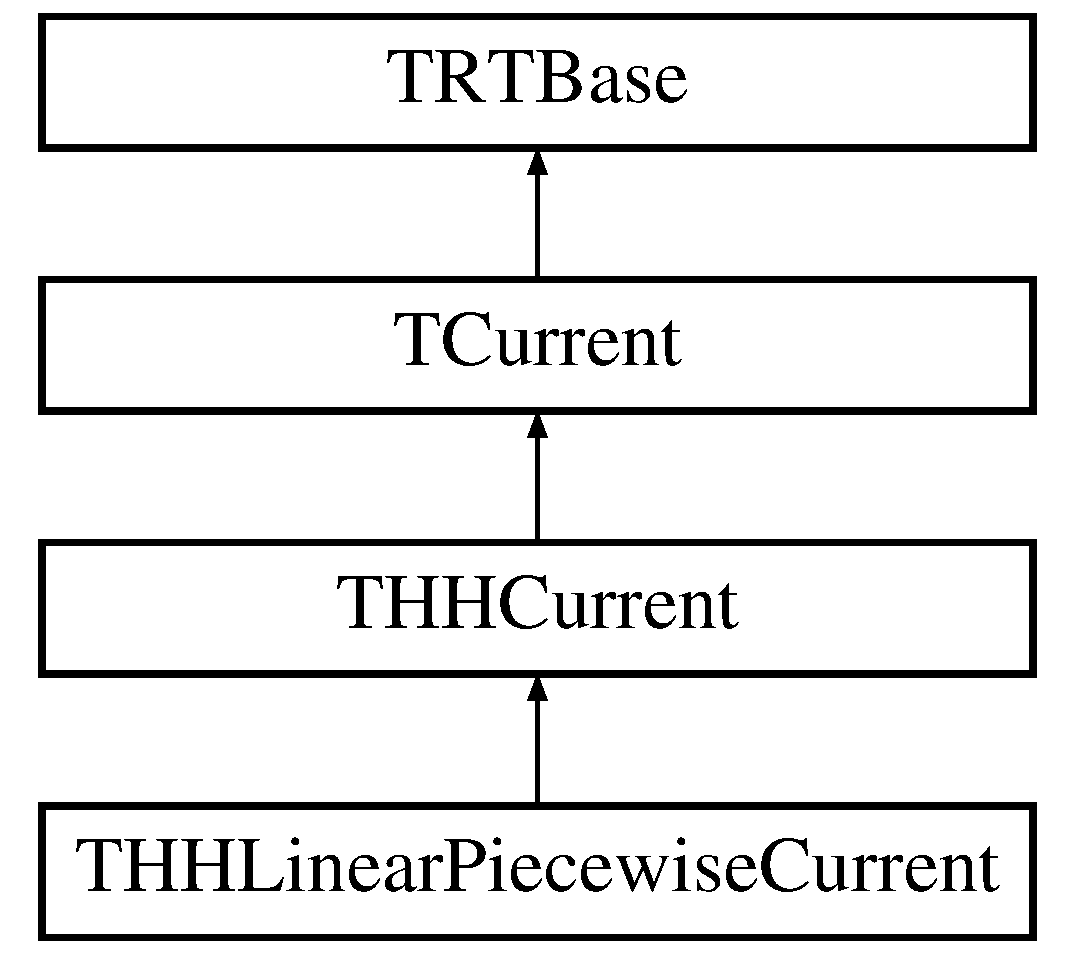
\includegraphics[height=4.000000cm]{class_t_h_h_linear_piecewise_current}
\end{center}
\end{figure}
\subsection*{Public Member Functions}
\begin{DoxyCompactItemize}
\item 
\hypertarget{class_t_h_h_linear_piecewise_current_a45566194697e4b2a9193ef4a3c715dca}{int {\bfseries get\+\_\+\+Use\+Vdrv} ()}\label{class_t_h_h_linear_piecewise_current_a45566194697e4b2a9193ef4a3c715dca}

\item 
\hypertarget{class_t_h_h_linear_piecewise_current_ae961f47da85a52182980389753cc3f51}{void {\bfseries set\+\_\+\+Use\+Vdrv} (int set)}\label{class_t_h_h_linear_piecewise_current_ae961f47da85a52182980389753cc3f51}

\item 
\hypertarget{class_t_h_h_linear_piecewise_current_a00c20e50ac6dc2b4ae4456647705b9f5}{\hyperlink{class_t_h_h_kinetics_factor}{T\+H\+H\+Kinetics\+Factor} \&\+\_\+\+\_\+fastcall \hyperlink{class_t_h_h_linear_piecewise_current_a00c20e50ac6dc2b4ae4456647705b9f5}{get\+\_\+m} ()}\label{class_t_h_h_linear_piecewise_current_a00c20e50ac6dc2b4ae4456647705b9f5}

\begin{DoxyCompactList}\small\item\em activation kinetic factor \end{DoxyCompactList}\item 
\hypertarget{class_t_h_h_linear_piecewise_current_afff1680475172a45ca812d591bcb91e3}{\hyperlink{class_t_h_h_kinetics_factor}{T\+H\+H\+Kinetics\+Factor} \&\+\_\+\+\_\+fastcall \hyperlink{class_t_h_h_linear_piecewise_current_afff1680475172a45ca812d591bcb91e3}{get\+\_\+h} ()}\label{class_t_h_h_linear_piecewise_current_afff1680475172a45ca812d591bcb91e3}

\begin{DoxyCompactList}\small\item\em inactivation kinetic factor \end{DoxyCompactList}\item 
\hypertarget{class_t_h_h_linear_piecewise_current_ace17759ac3ac09d2bc73f84ed240bc76}{\hyperlink{class_t_h_h_kinetics_factor}{T\+H\+H\+Kinetics\+Factor} \&\+\_\+\+\_\+fastcall \hyperlink{class_t_h_h_linear_piecewise_current_ace17759ac3ac09d2bc73f84ed240bc76}{get\+\_\+n} ()}\label{class_t_h_h_linear_piecewise_current_ace17759ac3ac09d2bc73f84ed240bc76}

\begin{DoxyCompactList}\small\item\em third kinetic factor \end{DoxyCompactList}\item 
\hypertarget{class_t_h_h_linear_piecewise_current_a9a240a941e2a98fc5bebf3ffb255541c}{void $\ast$const \+\_\+\+\_\+fastcall \hyperlink{class_t_h_h_linear_piecewise_current_a9a240a941e2a98fc5bebf3ffb255541c}{Get\+Edit\+Form} ()}\label{class_t_h_h_linear_piecewise_current_a9a240a941e2a98fc5bebf3ffb255541c}

\begin{DoxyCompactList}\small\item\em Returns downcasted T\+H\+H\+Current\+Form$\ast$ that is used to set values for this object. \end{DoxyCompactList}\item 
double \+\_\+\+\_\+fastcall \hyperlink{class_t_h_h_linear_piecewise_current_a7607b43e63ba9761d083aba7c25edfd6}{Do\+Update} (double step, double Vkin, double Vdrv, std\+::vector$<$ double $>$ \&params)
\begin{DoxyCompactList}\small\item\em Calculation of H\+H type current based on two voltages. \end{DoxyCompactList}\item 
\hypertarget{class_t_h_h_linear_piecewise_current_a38f06e164c879be3217bf28e0d4007eb}{void \+\_\+\+\_\+fastcall \hyperlink{class_t_h_h_linear_piecewise_current_a38f06e164c879be3217bf28e0d4007eb}{Populate\+Edit\+Form} ()}\label{class_t_h_h_linear_piecewise_current_a38f06e164c879be3217bf28e0d4007eb}

\begin{DoxyCompactList}\small\item\em Called by G\+U\+I to synchronize edit form with current values of object params. \end{DoxyCompactList}\item 
\hypertarget{class_t_h_h_linear_piecewise_current_ac3a70f25cf651fbd5325b3a58274ea6b}{bool \+\_\+\+\_\+fastcall \hyperlink{class_t_h_h_linear_piecewise_current_ac3a70f25cf651fbd5325b3a58274ea6b}{Validate\+Edit\+Form} ()}\label{class_t_h_h_linear_piecewise_current_ac3a70f25cf651fbd5325b3a58274ea6b}

\begin{DoxyCompactList}\small\item\em Called by G\+U\+I to check if changed values are satisfactory. \end{DoxyCompactList}\item 
\hypertarget{class_t_h_h_linear_piecewise_current_a31c5f0dc47ca42c6980fda9805a91bbf}{void const \+\_\+\+\_\+fastcall \hyperlink{class_t_h_h_linear_piecewise_current_a31c5f0dc47ca42c6980fda9805a91bbf}{Write\+To\+Stream} (ostream \&stream) const }\label{class_t_h_h_linear_piecewise_current_a31c5f0dc47ca42c6980fda9805a91bbf}

\begin{DoxyCompactList}\small\item\em Writes data members to a stream. \end{DoxyCompactList}\item 
\hypertarget{class_t_h_h_linear_piecewise_current_ab1b1960c579db90343e0fe262ec54554}{void const \+\_\+\+\_\+fastcall \hyperlink{class_t_h_h_linear_piecewise_current_ab1b1960c579db90343e0fe262ec54554}{Read\+From\+Stream} (istream \&stream)}\label{class_t_h_h_linear_piecewise_current_ab1b1960c579db90343e0fe262ec54554}

\begin{DoxyCompactList}\small\item\em Reads data members from a stream. \end{DoxyCompactList}\item 
const std\+::wstring \&\+\_\+\+\_\+fastcall \hyperlink{class_t_h_h_linear_piecewise_current_a2f62f65488ad9489bdf671b6fd4dd837}{Class\+Key} () const 
\begin{DoxyCompactList}\small\item\em Returns string used to register class with factory. \end{DoxyCompactList}\item 
\hypertarget{class_t_h_h_linear_piecewise_current_a92e36381784a3cc1d602187edf73ec9b}{\+\_\+\+\_\+fastcall \hyperlink{class_t_h_h_linear_piecewise_current_a92e36381784a3cc1d602187edf73ec9b}{T\+H\+H\+Linear\+Piecewise\+Current} ()}\label{class_t_h_h_linear_piecewise_current_a92e36381784a3cc1d602187edf73ec9b}

\begin{DoxyCompactList}\small\item\em default constructor \end{DoxyCompactList}\item 
\hypertarget{class_t_h_h_linear_piecewise_current_a8d38ff0fb0a254ad6209bcd168dc4697}{\+\_\+\+\_\+fastcall \hyperlink{class_t_h_h_linear_piecewise_current_a8d38ff0fb0a254ad6209bcd168dc4697}{T\+H\+H\+Linear\+Piecewise\+Current} (\hyperlink{class_t_current_user}{T\+Current\+User} $\ast$owner, const std\+::wstring \&name)}\label{class_t_h_h_linear_piecewise_current_a8d38ff0fb0a254ad6209bcd168dc4697}

\begin{DoxyCompactList}\small\item\em specialized constructor 2 param \end{DoxyCompactList}\item 
\hypertarget{class_t_h_h_linear_piecewise_current_ac68b67b8c8cbaeadad49b8b70f4e8163}{\+\_\+\+\_\+fastcall \hyperlink{class_t_h_h_linear_piecewise_current_ac68b67b8c8cbaeadad49b8b70f4e8163}{T\+H\+H\+Linear\+Piecewise\+Current} (const std\+::wstring \&name)}\label{class_t_h_h_linear_piecewise_current_ac68b67b8c8cbaeadad49b8b70f4e8163}

\begin{DoxyCompactList}\small\item\em specialized constructor 1 param \end{DoxyCompactList}\item 
\hypertarget{class_t_h_h_linear_piecewise_current_a0f475541235ceab6e40af3aa6527e9e5}{\+\_\+\+\_\+fastcall \hyperlink{class_t_h_h_linear_piecewise_current_a0f475541235ceab6e40af3aa6527e9e5}{T\+H\+H\+Linear\+Piecewise\+Current} (const \hyperlink{class_t_h_h_linear_piecewise_current}{T\+H\+H\+Linear\+Piecewise\+Current} \&source)}\label{class_t_h_h_linear_piecewise_current_a0f475541235ceab6e40af3aa6527e9e5}

\begin{DoxyCompactList}\small\item\em copy constructor \end{DoxyCompactList}\item 
\hypertarget{class_t_h_h_linear_piecewise_current_a4000d88fe350057e43d165737419b816}{\hyperlink{class_t_h_h_linear_piecewise_current}{T\+H\+H\+Linear\+Piecewise\+Current} \& \hyperlink{class_t_h_h_linear_piecewise_current_a4000d88fe350057e43d165737419b816}{operator=} (const \hyperlink{class_t_h_h_linear_piecewise_current}{T\+H\+H\+Linear\+Piecewise\+Current} \&source)}\label{class_t_h_h_linear_piecewise_current_a4000d88fe350057e43d165737419b816}

\begin{DoxyCompactList}\small\item\em overloaded assignment operator \end{DoxyCompactList}\item 
\hypertarget{class_t_h_h_linear_piecewise_current_a884f539c84bd751b9411078cc70cca21}{void \+\_\+\+\_\+fastcall \hyperlink{class_t_h_h_linear_piecewise_current_a884f539c84bd751b9411078cc70cca21}{Copy\+Params\+From} (const \hyperlink{class_t_current}{T\+Current} $\ast$const source)}\label{class_t_h_h_linear_piecewise_current_a884f539c84bd751b9411078cc70cca21}

\begin{DoxyCompactList}\small\item\em overloaded method for duplicating currents without complete assignment \end{DoxyCompactList}\end{DoxyCompactItemize}
\subsection*{Friends}
\begin{DoxyCompactItemize}
\item 
\hypertarget{class_t_h_h_linear_piecewise_current_ac98d07dd8f7b70e16ccb9a01abf56b9c}{class {\bfseries boost\+::serialization\+::access}}\label{class_t_h_h_linear_piecewise_current_ac98d07dd8f7b70e16ccb9a01abf56b9c}

\end{DoxyCompactItemize}
\subsection*{Additional Inherited Members}


\subsection{Detailed Description}
Implementation of Hodgkin-\/\+Huxley type current with Tohidi-\/\+Nadim shortcuts. 


\begin{DoxyPre}
 Classes \hyperlink{class_t_h_h_linear_piecewise_current}{THHLinearPiecewiseCurrent} gives ionic current as a function of several kinetic
 parameters and the input voltages V\_kin and V\_drv.  For intrinsic currents V\_drv = V\_kin,
 and for synaptic currents, V\_kin is the voltage of the presynaptic cell.\end{DoxyPre}



\begin{DoxyPre} A new parameter, UseVdrv, is introduced that determines whether the current is
 dependent on the driving force, V\_drv - E.\end{DoxyPre}



\begin{DoxyPre} if UseVdrv = 1
                             p   q   r
 computes I = Gmax * m * h * n * (V\_drv - E)\end{DoxyPre}



\begin{DoxyPre} if UseVdrv = 0
                             p   q   r
 computes I = Gmax * m * h * n\end{DoxyPre}



\begin{DoxyPre}\end{DoxyPre}


\begin{DoxyAuthor}{Author}
E. Brady Trexler $<$ebtrexler (at) gothamsci.\+com$>$, 2011 -\/ 2014 
\end{DoxyAuthor}


\subsection{Member Function Documentation}
\hypertarget{class_t_h_h_linear_piecewise_current_a2f62f65488ad9489bdf671b6fd4dd837}{\index{T\+H\+H\+Linear\+Piecewise\+Current@{T\+H\+H\+Linear\+Piecewise\+Current}!Class\+Key@{Class\+Key}}
\index{Class\+Key@{Class\+Key}!T\+H\+H\+Linear\+Piecewise\+Current@{T\+H\+H\+Linear\+Piecewise\+Current}}
\subsubsection[{Class\+Key}]{\setlength{\rightskip}{0pt plus 5cm}const std\+::wstring\& \+\_\+\+\_\+fastcall T\+H\+H\+Linear\+Piecewise\+Current\+::\+Class\+Key (
\begin{DoxyParamCaption}
{}
\end{DoxyParamCaption}
) const\hspace{0.3cm}{\ttfamily [inline]}, {\ttfamily [virtual]}}}\label{class_t_h_h_linear_piecewise_current_a2f62f65488ad9489bdf671b6fd4dd837}


Returns string used to register class with factory. 

Users of class factories must also tell the class the key they used when registering the class. See factory.\+h 

Reimplemented from \hyperlink{class_t_h_h_current_a49049acfa420622d26011f881c432329}{T\+H\+H\+Current}.

\hypertarget{class_t_h_h_linear_piecewise_current_a7607b43e63ba9761d083aba7c25edfd6}{\index{T\+H\+H\+Linear\+Piecewise\+Current@{T\+H\+H\+Linear\+Piecewise\+Current}!Do\+Update@{Do\+Update}}
\index{Do\+Update@{Do\+Update}!T\+H\+H\+Linear\+Piecewise\+Current@{T\+H\+H\+Linear\+Piecewise\+Current}}
\subsubsection[{Do\+Update}]{\setlength{\rightskip}{0pt plus 5cm}double \+\_\+\+\_\+fastcall T\+H\+H\+Linear\+Piecewise\+Current\+::\+Do\+Update (
\begin{DoxyParamCaption}
\item[{double}]{step, }
\item[{double}]{Vkin, }
\item[{double}]{Vdrv, }
\item[{std\+::vector$<$ double $>$ \&}]{params}
\end{DoxyParamCaption}
)\hspace{0.3cm}{\ttfamily [inline]}, {\ttfamily [virtual]}}}\label{class_t_h_h_linear_piecewise_current_a7607b43e63ba9761d083aba7c25edfd6}


Calculation of H\+H type current based on two voltages. 


\begin{DoxyPre}
                                     p         q         r
          computes I = Gmax * m(Vkin) * h(Vkin) * n(Vkin) * (Vdrv - E)   or
\begin{DoxyVerb}                       p         q         r
\end{DoxyVerb}

          computes I = Gmax * m(Vkin) * h(Vkin) * n(Vkin)\end{DoxyPre}



\begin{DoxyPre}            depending on UseVdrv setting
\end{DoxyPre}
 

Reimplemented from \hyperlink{class_t_h_h_current_acaa8176752a6ccc45611d0c80b1a971a}{T\+H\+H\+Current}.



The documentation for this class was generated from the following file\+:\begin{DoxyCompactItemize}
\item 
R\+T\+\_\+\+H\+H\+Linear\+Piecewise\+Current.\+cpp\end{DoxyCompactItemize}

\hypertarget{class_t_h_h_linear_piecewise_kinetics_factor}{\section{T\+H\+H\+Linear\+Piecewise\+Kinetics\+Factor Class Reference}
\label{class_t_h_h_linear_piecewise_kinetics_factor}\index{T\+H\+H\+Linear\+Piecewise\+Kinetics\+Factor@{T\+H\+H\+Linear\+Piecewise\+Kinetics\+Factor}}
}


Kinetic factor used by \hyperlink{class_t_h_h_linear_piecewise_current}{T\+H\+H\+Linear\+Piecewise\+Current}.  




{\ttfamily \#include $<$R\+T\+\_\+\+H\+H\+Linear\+Piecewise\+Kinetics\+Factor.\+h$>$}

Inheritance diagram for T\+H\+H\+Linear\+Piecewise\+Kinetics\+Factor\+:\begin{figure}[H]
\begin{center}
\leavevmode
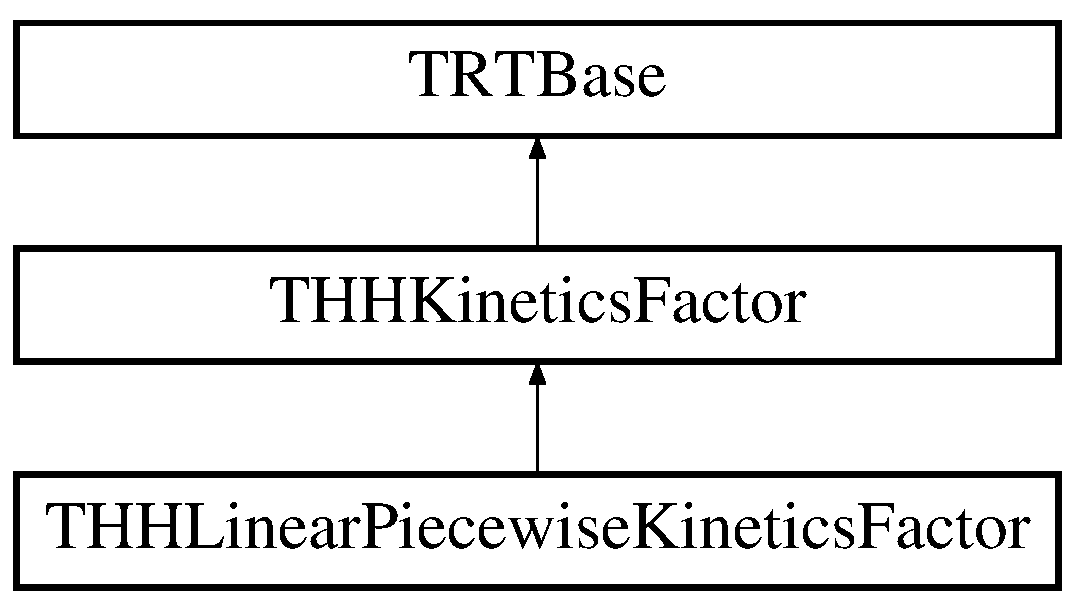
\includegraphics[height=3.000000cm]{class_t_h_h_linear_piecewise_kinetics_factor}
\end{center}
\end{figure}
\subsection*{Public Member Functions}
\begin{DoxyCompactItemize}
\item 
const std\+::wstring \&\+\_\+\+\_\+fastcall \hyperlink{class_t_h_h_linear_piecewise_kinetics_factor_a2129c509478fcca9cb2479817856c0bf}{Class\+Key} () const 
\begin{DoxyCompactList}\small\item\em Returns string used to register class with factory. \end{DoxyCompactList}\item 
\hypertarget{class_t_h_h_linear_piecewise_kinetics_factor_afb243ba364ac0e3f52b2859b41d03b49}{virtual double \hyperlink{class_t_h_h_linear_piecewise_kinetics_factor_afb243ba364ac0e3f52b2859b41d03b49}{tau} (double V)}\label{class_t_h_h_linear_piecewise_kinetics_factor_afb243ba364ac0e3f52b2859b41d03b49}

\begin{DoxyCompactList}\small\item\em Calculates new value of tau from given voltage, V. \end{DoxyCompactList}\item 
\hypertarget{class_t_h_h_linear_piecewise_kinetics_factor_a351152558aaa57d4d1ad76f8678be006}{virtual double \hyperlink{class_t_h_h_linear_piecewise_kinetics_factor_a351152558aaa57d4d1ad76f8678be006}{inf} (double V)}\label{class_t_h_h_linear_piecewise_kinetics_factor_a351152558aaa57d4d1ad76f8678be006}

\begin{DoxyCompactList}\small\item\em Calculates new value of inf from given voltage, V. \end{DoxyCompactList}\item 
\hypertarget{class_t_h_h_linear_piecewise_kinetics_factor_a715ee195ff8f19488a7a8ea96b91ee84}{\+\_\+\+\_\+fastcall \hyperlink{class_t_h_h_linear_piecewise_kinetics_factor_a715ee195ff8f19488a7a8ea96b91ee84}{T\+H\+H\+Linear\+Piecewise\+Kinetics\+Factor} ()}\label{class_t_h_h_linear_piecewise_kinetics_factor_a715ee195ff8f19488a7a8ea96b91ee84}

\begin{DoxyCompactList}\small\item\em default constructor \end{DoxyCompactList}\item 
\hypertarget{class_t_h_h_linear_piecewise_kinetics_factor_ae0f4efc8e965d584fca76c719bbc4ebf}{\+\_\+\+\_\+fastcall \hyperlink{class_t_h_h_linear_piecewise_kinetics_factor_ae0f4efc8e965d584fca76c719bbc4ebf}{T\+H\+H\+Linear\+Piecewise\+Kinetics\+Factor} (const \hyperlink{class_t_h_h_linear_piecewise_kinetics_factor}{T\+H\+H\+Linear\+Piecewise\+Kinetics\+Factor} \&source)}\label{class_t_h_h_linear_piecewise_kinetics_factor_ae0f4efc8e965d584fca76c719bbc4ebf}

\begin{DoxyCompactList}\small\item\em copy constructor \end{DoxyCompactList}\item 
\hypertarget{class_t_h_h_linear_piecewise_kinetics_factor_a9ba6e423ce1840c05795bff77aab10f3}{\hyperlink{class_t_h_h_linear_piecewise_kinetics_factor}{T\+H\+H\+Linear\+Piecewise\+Kinetics\+Factor} \& \hyperlink{class_t_h_h_linear_piecewise_kinetics_factor_a9ba6e423ce1840c05795bff77aab10f3}{operator=} (const \hyperlink{class_t_h_h_linear_piecewise_kinetics_factor}{T\+H\+H\+Linear\+Piecewise\+Kinetics\+Factor} \&source)}\label{class_t_h_h_linear_piecewise_kinetics_factor_a9ba6e423ce1840c05795bff77aab10f3}

\begin{DoxyCompactList}\small\item\em overloaded assignment operator \end{DoxyCompactList}\item 
\hypertarget{class_t_h_h_linear_piecewise_kinetics_factor_a00b0a552987402d93499975e01d9bcaf}{virtual void \+\_\+\+\_\+fastcall \hyperlink{class_t_h_h_linear_piecewise_kinetics_factor_a00b0a552987402d93499975e01d9bcaf}{Populate\+Params} (void $\ast$gui\+Element)}\label{class_t_h_h_linear_piecewise_kinetics_factor_a00b0a552987402d93499975e01d9bcaf}

\begin{DoxyCompactList}\small\item\em Fill in param names for G\+U\+I. \end{DoxyCompactList}\item 
\hypertarget{class_t_h_h_linear_piecewise_kinetics_factor_ae4bcfffda552e54170faf1d2737cfb15}{virtual bool \+\_\+\+\_\+fastcall \hyperlink{class_t_h_h_linear_piecewise_kinetics_factor_ae4bcfffda552e54170faf1d2737cfb15}{Kinetic\+Factors\+Validate} (\hyperlink{class_t_h_h_kinetics_factor}{T\+H\+H\+Kinetics\+Factor} \&\hyperlink{class_t_h_h_kinetics_factor_aa58fa2b2da61a14dd674f22d32a62248}{f}, wchar\+\_\+t $\ast$factorname, void $\ast$ed, double \&the\+\_\+exp, wchar\+\_\+t $\ast$exptext)}\label{class_t_h_h_linear_piecewise_kinetics_factor_ae4bcfffda552e54170faf1d2737cfb15}

\begin{DoxyCompactList}\small\item\em called by Validate\+Edit\+Form \end{DoxyCompactList}\end{DoxyCompactItemize}
\subsection*{Public Attributes}
\begin{DoxyCompactItemize}
\item 
\hypertarget{class_t_h_h_linear_piecewise_kinetics_factor_a64c5bc29239227eaaa3ea0b0ae618502}{\+\_\+\+\_\+property double \hyperlink{class_t_h_h_linear_piecewise_kinetics_factor_a64c5bc29239227eaaa3ea0b0ae618502}{V\+\_\+lo} = \{read = F\+\_\+\+V\+\_\+lo, write = F\+\_\+\+V\+\_\+lo\}}\label{class_t_h_h_linear_piecewise_kinetics_factor_a64c5bc29239227eaaa3ea0b0ae618502}

\begin{DoxyCompactList}\small\item\em lower bounds voltage \end{DoxyCompactList}\item 
\hypertarget{class_t_h_h_linear_piecewise_kinetics_factor_aa9b1e3cabc1f97b189eda776db677836}{\+\_\+\+\_\+property double \hyperlink{class_t_h_h_linear_piecewise_kinetics_factor_aa9b1e3cabc1f97b189eda776db677836}{V\+\_\+hi} = \{read = F\+\_\+\+V\+\_\+hi, write = F\+\_\+\+V\+\_\+hi\}}\label{class_t_h_h_linear_piecewise_kinetics_factor_aa9b1e3cabc1f97b189eda776db677836}

\begin{DoxyCompactList}\small\item\em upper bounds voltage \end{DoxyCompactList}\item 
\hypertarget{class_t_h_h_linear_piecewise_kinetics_factor_a1accd3668b53a88fa047c17695f8b6a7}{\+\_\+\+\_\+property double \hyperlink{class_t_h_h_linear_piecewise_kinetics_factor_a1accd3668b53a88fa047c17695f8b6a7}{slope} = \{read = F\+\_\+slope, write = F\+\_\+slope\}}\label{class_t_h_h_linear_piecewise_kinetics_factor_a1accd3668b53a88fa047c17695f8b6a7}

\begin{DoxyCompactList}\small\item\em slope of interpolation line \end{DoxyCompactList}\item 
\hypertarget{class_t_h_h_linear_piecewise_kinetics_factor_ab71596e55e35b7f1562b01ef46f0ed98}{\+\_\+\+\_\+property double \hyperlink{class_t_h_h_linear_piecewise_kinetics_factor_ab71596e55e35b7f1562b01ef46f0ed98}{intcpt} = \{read = F\+\_\+intcpt, write = F\+\_\+intcpt\}}\label{class_t_h_h_linear_piecewise_kinetics_factor_ab71596e55e35b7f1562b01ef46f0ed98}

\begin{DoxyCompactList}\small\item\em intercept of interpolation line \end{DoxyCompactList}\item 
\hypertarget{class_t_h_h_linear_piecewise_kinetics_factor_a84c7ea0344463455e6b35eb4c679f1a2}{\+\_\+\+\_\+property double \hyperlink{class_t_h_h_linear_piecewise_kinetics_factor_a84c7ea0344463455e6b35eb4c679f1a2}{t\+\_\+lo} = \{read = F\+\_\+t\+\_\+lo, write = F\+\_\+t\+\_\+lo\}}\label{class_t_h_h_linear_piecewise_kinetics_factor_a84c7ea0344463455e6b35eb4c679f1a2}

\begin{DoxyCompactList}\small\item\em Tau = t\+\_\+lo if V $<$ V\+\_\+lo. \end{DoxyCompactList}\item 
\hypertarget{class_t_h_h_linear_piecewise_kinetics_factor_a37584a8a4d82b84d7c56ba1f3b44f97a}{\+\_\+\+\_\+property double \hyperlink{class_t_h_h_linear_piecewise_kinetics_factor_a37584a8a4d82b84d7c56ba1f3b44f97a}{t\+\_\+hi} = \{read = F\+\_\+t\+\_\+hi, write = F\+\_\+t\+\_\+hi\}}\label{class_t_h_h_linear_piecewise_kinetics_factor_a37584a8a4d82b84d7c56ba1f3b44f97a}

\begin{DoxyCompactList}\small\item\em Tau = t\+\_\+hi if V $>$ V\+\_\+hi. \end{DoxyCompactList}\item 
\hypertarget{class_t_h_h_linear_piecewise_kinetics_factor_a5e6df3d4e2c80f117f9a453035975a18}{\+\_\+\+\_\+property double \hyperlink{class_t_h_h_linear_piecewise_kinetics_factor_a5e6df3d4e2c80f117f9a453035975a18}{y\+\_\+n} = \{read = F\+\_\+y\+\_\+n, write = F\+\_\+y\+\_\+n\}}\label{class_t_h_h_linear_piecewise_kinetics_factor_a5e6df3d4e2c80f117f9a453035975a18}

\begin{DoxyCompactList}\small\item\em Value of the updated parameter at the end of a step. \end{DoxyCompactList}\end{DoxyCompactItemize}
\subsection*{Protected Member Functions}
\begin{DoxyCompactItemize}
\item 
\hypertarget{class_t_h_h_linear_piecewise_kinetics_factor_ad3fc61149df1a12c58e7c3f5df3bd52c}{virtual void const \+\_\+\+\_\+fastcall \hyperlink{class_t_h_h_linear_piecewise_kinetics_factor_ad3fc61149df1a12c58e7c3f5df3bd52c}{Write\+To\+Stream} (ostream \&stream) const }\label{class_t_h_h_linear_piecewise_kinetics_factor_ad3fc61149df1a12c58e7c3f5df3bd52c}

\begin{DoxyCompactList}\small\item\em Writes data members to a stream. \end{DoxyCompactList}\item 
\hypertarget{class_t_h_h_linear_piecewise_kinetics_factor_ad6fa7a818f89fc488d06af4af2f9f1f6}{virtual void const \+\_\+\+\_\+fastcall \hyperlink{class_t_h_h_linear_piecewise_kinetics_factor_ad6fa7a818f89fc488d06af4af2f9f1f6}{Read\+From\+Stream} (istream \&stream)}\label{class_t_h_h_linear_piecewise_kinetics_factor_ad6fa7a818f89fc488d06af4af2f9f1f6}

\begin{DoxyCompactList}\small\item\em Reads data members from a stream. \end{DoxyCompactList}\end{DoxyCompactItemize}
\subsection*{Friends}
\begin{DoxyCompactItemize}
\item 
\hypertarget{class_t_h_h_linear_piecewise_kinetics_factor_ac98d07dd8f7b70e16ccb9a01abf56b9c}{class {\bfseries boost\+::serialization\+::access}}\label{class_t_h_h_linear_piecewise_kinetics_factor_ac98d07dd8f7b70e16ccb9a01abf56b9c}

\end{DoxyCompactItemize}


\subsection{Detailed Description}
Kinetic factor used by \hyperlink{class_t_h_h_linear_piecewise_current}{T\+H\+H\+Linear\+Piecewise\+Current}. 


\begin{DoxyPre}
     This class implements a Hodgkin-Huxley based current with the modification
     that tau and inf are linear and piecewise, where\end{DoxyPre}



\begin{DoxyPre}    xinf(V)    =    a*V+b    if Vlo <= V <= Vhi
                  =    a*Vlo+b  if V < Vlo
                  =    a*Vhi+b  if  V > Vhi\end{DoxyPre}



\begin{DoxyPre}    xtau(V)    =    a*V+b    if Vlo <= V <= Vhi
                  =    a*Vlo+b  if V < Vlo
                  =    a*Vhi+b  if  V > Vhi\end{DoxyPre}



\begin{DoxyPre}    a is the slope and b is the intercept of the line\end{DoxyPre}



\begin{DoxyPre}\end{DoxyPre}


\begin{DoxyAuthor}{Author}
E. Brady Trexler $<$ebtrexler (at) gothamsci.\+com$>$, 2011 -\/ 2014 
\end{DoxyAuthor}


\subsection{Member Function Documentation}
\hypertarget{class_t_h_h_linear_piecewise_kinetics_factor_a2129c509478fcca9cb2479817856c0bf}{\index{T\+H\+H\+Linear\+Piecewise\+Kinetics\+Factor@{T\+H\+H\+Linear\+Piecewise\+Kinetics\+Factor}!Class\+Key@{Class\+Key}}
\index{Class\+Key@{Class\+Key}!T\+H\+H\+Linear\+Piecewise\+Kinetics\+Factor@{T\+H\+H\+Linear\+Piecewise\+Kinetics\+Factor}}
\subsubsection[{Class\+Key}]{\setlength{\rightskip}{0pt plus 5cm}const std\+::wstring\& \+\_\+\+\_\+fastcall T\+H\+H\+Linear\+Piecewise\+Kinetics\+Factor\+::\+Class\+Key (
\begin{DoxyParamCaption}
{}
\end{DoxyParamCaption}
) const\hspace{0.3cm}{\ttfamily [inline]}, {\ttfamily [virtual]}}}\label{class_t_h_h_linear_piecewise_kinetics_factor_a2129c509478fcca9cb2479817856c0bf}


Returns string used to register class with factory. 

Users of class factories must also tell the class the key they used when registering the class. See factory.\+h 

Reimplemented from \hyperlink{class_t_h_h_kinetics_factor_ac161d432e14597146b0bd45cbed7e225}{T\+H\+H\+Kinetics\+Factor}.



The documentation for this class was generated from the following files\+:\begin{DoxyCompactItemize}
\item 
R\+T\+\_\+\+H\+H\+Linear\+Piecewise\+Kinetics\+Factor.\+h\item 
R\+T\+\_\+\+H\+H\+Linear\+Piecewise\+Kinetics\+Factor.\+cpp\end{DoxyCompactItemize}

\hypertarget{class_t_injection_electrode}{\section{T\+Injection\+Electrode Class Reference}
\label{class_t_injection_electrode}\index{T\+Injection\+Electrode@{T\+Injection\+Electrode}}
}


Implementation of a simple square-\/wave current pulse.  


Inheritance diagram for T\+Injection\+Electrode\+:\begin{figure}[H]
\begin{center}
\leavevmode
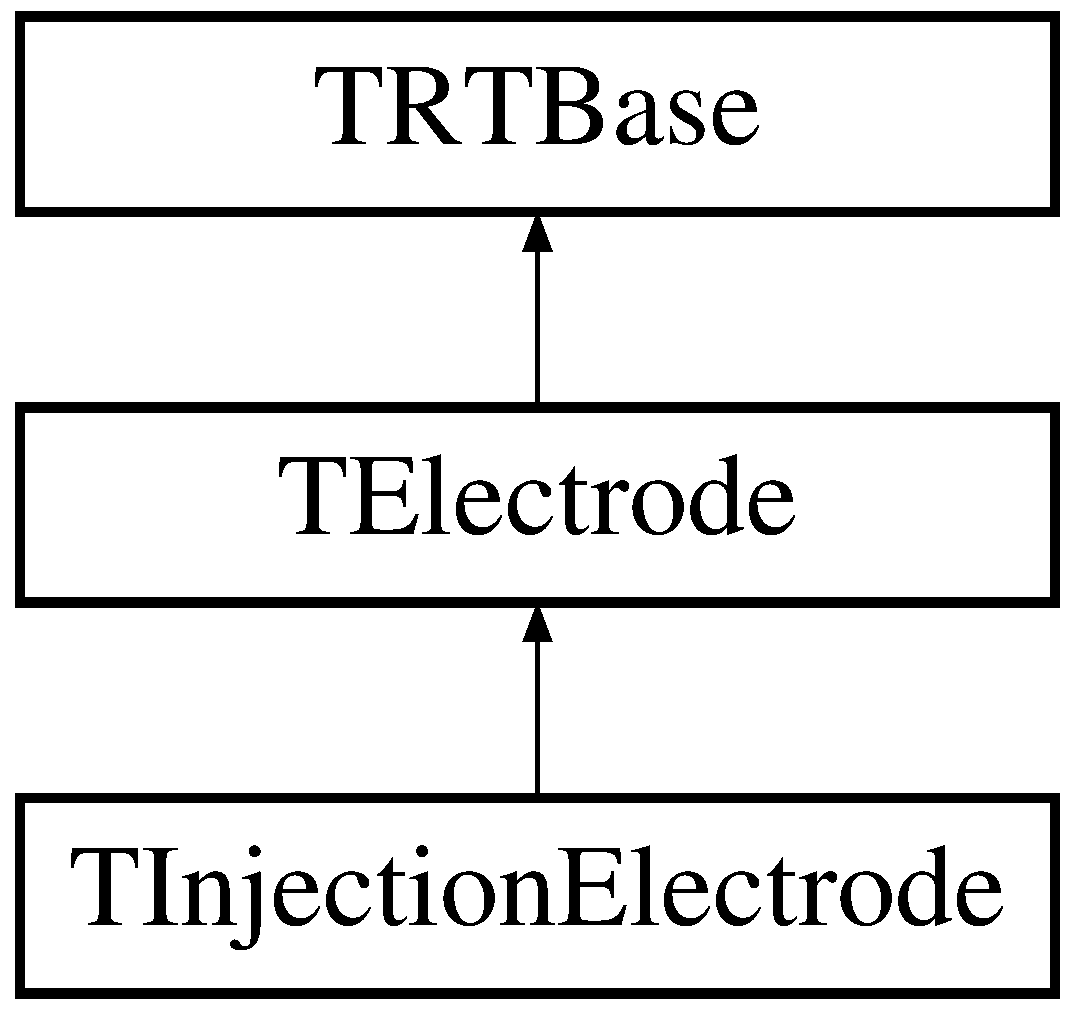
\includegraphics[height=3.000000cm]{class_t_injection_electrode}
\end{center}
\end{figure}
\subsection*{Public Member Functions}
\begin{DoxyCompactItemize}
\item 
\hypertarget{class_t_injection_electrode_ae39c315dc50e675e69681aaf5efb9bb6}{bool \+\_\+\+\_\+fastcall \hyperlink{class_t_injection_electrode_ae39c315dc50e675e69681aaf5efb9bb6}{Initialize} (bool Reset)}\label{class_t_injection_electrode_ae39c315dc50e675e69681aaf5efb9bb6}

\begin{DoxyCompactList}\small\item\em Initializes .... \end{DoxyCompactList}\item 
const std\+::wstring \&\+\_\+\+\_\+fastcall \hyperlink{class_t_injection_electrode_ad13dada3837856466fd9321afee58166}{Class\+Key} () const 
\begin{DoxyCompactList}\small\item\em Returns string used to register class with factory. \end{DoxyCompactList}\item 
virtual double \+\_\+\+\_\+fastcall \hyperlink{class_t_injection_electrode_a4d5b8d7c4c1dc5d9290ca8456c3be24b}{Do\+Update} (double step)
\begin{DoxyCompactList}\small\item\em Calculation of injected current based on step. \end{DoxyCompactList}\item 
\hypertarget{class_t_injection_electrode_a48a2e40fcd0a954b99dc7b70a930befc}{virtual void \+\_\+\+\_\+fastcall \hyperlink{class_t_injection_electrode_a48a2e40fcd0a954b99dc7b70a930befc}{Populate\+Edit\+Form} ()}\label{class_t_injection_electrode_a48a2e40fcd0a954b99dc7b70a930befc}

\begin{DoxyCompactList}\small\item\em Called by G\+U\+I to synchronize edit form with current values of object params. \end{DoxyCompactList}\item 
\hypertarget{class_t_injection_electrode_afd51d63f30eb2fbdb2c53ca09e11714e}{virtual bool \+\_\+\+\_\+fastcall \hyperlink{class_t_injection_electrode_afd51d63f30eb2fbdb2c53ca09e11714e}{Validate\+Edit\+Form} ()}\label{class_t_injection_electrode_afd51d63f30eb2fbdb2c53ca09e11714e}

\begin{DoxyCompactList}\small\item\em Called by G\+U\+I to check if changed values are satisfactory. \end{DoxyCompactList}\item 
\hypertarget{class_t_injection_electrode_a825ef8d17c3e3612aeb6b53c9e3aa539}{virtual void $\ast$const \+\_\+\+\_\+fastcall \hyperlink{class_t_injection_electrode_a825ef8d17c3e3612aeb6b53c9e3aa539}{Get\+Edit\+Form} ()}\label{class_t_injection_electrode_a825ef8d17c3e3612aeb6b53c9e3aa539}

\begin{DoxyCompactList}\small\item\em Returns downcasted T\+Injection\+Electrode\+Form$\ast$ that is used to set values for this object. \end{DoxyCompactList}\item 
\hypertarget{class_t_injection_electrode_a804cd0834dd64ce2cc0ff9ef828a2d81}{\+\_\+\+\_\+fastcall \hyperlink{class_t_injection_electrode_a804cd0834dd64ce2cc0ff9ef828a2d81}{T\+Injection\+Electrode} ()}\label{class_t_injection_electrode_a804cd0834dd64ce2cc0ff9ef828a2d81}

\begin{DoxyCompactList}\small\item\em default constructor \end{DoxyCompactList}\item 
\hypertarget{class_t_injection_electrode_aac37df3fe47e264e2f5314025de25499}{\+\_\+\+\_\+fastcall \hyperlink{class_t_injection_electrode_aac37df3fe47e264e2f5314025de25499}{T\+Injection\+Electrode} (\hyperlink{class_t_cell}{T\+Cell} $\ast$const owner, const std\+::wstring \&name)}\label{class_t_injection_electrode_aac37df3fe47e264e2f5314025de25499}

\begin{DoxyCompactList}\small\item\em specialized constructor 2 param \end{DoxyCompactList}\item 
\hypertarget{class_t_injection_electrode_aa897a09ecd4e2697eb782c311de032d2}{\+\_\+\+\_\+fastcall \hyperlink{class_t_injection_electrode_aa897a09ecd4e2697eb782c311de032d2}{T\+Injection\+Electrode} (const std\+::wstring \&name)}\label{class_t_injection_electrode_aa897a09ecd4e2697eb782c311de032d2}

\begin{DoxyCompactList}\small\item\em specialized constructor 1 param \end{DoxyCompactList}\item 
\hypertarget{class_t_injection_electrode_ac8f9c7ae8dfa4894906dbed1cb1040ed}{\+\_\+\+\_\+fastcall \hyperlink{class_t_injection_electrode_ac8f9c7ae8dfa4894906dbed1cb1040ed}{T\+Injection\+Electrode} (const \hyperlink{class_t_injection_electrode}{T\+Injection\+Electrode} \&source)}\label{class_t_injection_electrode_ac8f9c7ae8dfa4894906dbed1cb1040ed}

\begin{DoxyCompactList}\small\item\em copy constructor \end{DoxyCompactList}\item 
\hypertarget{class_t_injection_electrode_a7eccc985aa8ae9c6f81c1aa618286a2f}{\hyperlink{class_t_injection_electrode}{T\+Injection\+Electrode} \& \hyperlink{class_t_injection_electrode_a7eccc985aa8ae9c6f81c1aa618286a2f}{operator=} (const \hyperlink{class_t_injection_electrode}{T\+Injection\+Electrode} \&source)}\label{class_t_injection_electrode_a7eccc985aa8ae9c6f81c1aa618286a2f}

\begin{DoxyCompactList}\small\item\em overloaded assignment operator \end{DoxyCompactList}\end{DoxyCompactItemize}
\subsection*{Protected Member Functions}
\begin{DoxyCompactItemize}
\item 
\hypertarget{class_t_injection_electrode_ac2358b8eca327bb7678b191ba36d7976}{virtual void const \+\_\+\+\_\+fastcall \hyperlink{class_t_injection_electrode_ac2358b8eca327bb7678b191ba36d7976}{Write\+To\+Stream} (ostream \&stream) const }\label{class_t_injection_electrode_ac2358b8eca327bb7678b191ba36d7976}

\begin{DoxyCompactList}\small\item\em Writes data members to a stream. \end{DoxyCompactList}\item 
\hypertarget{class_t_injection_electrode_a0eb782e62fe8505ac067d67d3dad88a2}{virtual void const \+\_\+\+\_\+fastcall \hyperlink{class_t_injection_electrode_a0eb782e62fe8505ac067d67d3dad88a2}{Read\+From\+Stream} (istream \&stream)}\label{class_t_injection_electrode_a0eb782e62fe8505ac067d67d3dad88a2}

\begin{DoxyCompactList}\small\item\em Reads data members from a stream. \end{DoxyCompactList}\end{DoxyCompactItemize}
\subsection*{Friends}
\begin{DoxyCompactItemize}
\item 
\hypertarget{class_t_injection_electrode_ac98d07dd8f7b70e16ccb9a01abf56b9c}{class {\bfseries boost\+::serialization\+::access}}\label{class_t_injection_electrode_ac98d07dd8f7b70e16ccb9a01abf56b9c}

\end{DoxyCompactItemize}


\subsection{Detailed Description}
Implementation of a simple square-\/wave current pulse. 


\begin{DoxyPre}
 Class \hyperlink{class_t_injection_electrode}{TInjectionElectrode} produces a square current in a cell.  The usual
 parameter settings are available, such as
   InitialDelay,
   Delay,
   Duration,
   Amplitude, and
   NumberOfRepeats
\end{DoxyPre}


\begin{DoxyAuthor}{Author}
E. Brady Trexler $<$ebtrexler (at) gothamsci.\+com$>$, 2011 -\/ 2013 
\end{DoxyAuthor}


\subsection{Member Function Documentation}
\hypertarget{class_t_injection_electrode_ad13dada3837856466fd9321afee58166}{\index{T\+Injection\+Electrode@{T\+Injection\+Electrode}!Class\+Key@{Class\+Key}}
\index{Class\+Key@{Class\+Key}!T\+Injection\+Electrode@{T\+Injection\+Electrode}}
\subsubsection[{Class\+Key}]{\setlength{\rightskip}{0pt plus 5cm}const std\+::wstring\& \+\_\+\+\_\+fastcall T\+Injection\+Electrode\+::\+Class\+Key (
\begin{DoxyParamCaption}
{}
\end{DoxyParamCaption}
) const\hspace{0.3cm}{\ttfamily [inline]}, {\ttfamily [virtual]}}}\label{class_t_injection_electrode_ad13dada3837856466fd9321afee58166}


Returns string used to register class with factory. 

Users of class factories must also tell the class the key they used when registering the class. See factory.\+h 

Implements \hyperlink{class_t_r_t_base_a6083fd510cbcb00faa85e5934fc3c18e}{T\+R\+T\+Base}.

\hypertarget{class_t_injection_electrode_a4d5b8d7c4c1dc5d9290ca8456c3be24b}{\index{T\+Injection\+Electrode@{T\+Injection\+Electrode}!Do\+Update@{Do\+Update}}
\index{Do\+Update@{Do\+Update}!T\+Injection\+Electrode@{T\+Injection\+Electrode}}
\subsubsection[{Do\+Update}]{\setlength{\rightskip}{0pt plus 5cm}virtual double \+\_\+\+\_\+fastcall T\+Injection\+Electrode\+::\+Do\+Update (
\begin{DoxyParamCaption}
\item[{double}]{step}
\end{DoxyParamCaption}
)\hspace{0.3cm}{\ttfamily [inline]}, {\ttfamily [virtual]}}}\label{class_t_injection_electrode_a4d5b8d7c4c1dc5d9290ca8456c3be24b}


Calculation of injected current based on step. 

Injection\+Electrode remembers the elapsed time and injects current according to desired waveform 

Implements \hyperlink{class_t_electrode_a3b535fa8d277cf8245f99900fc32ce99}{T\+Electrode}.



The documentation for this class was generated from the following file\+:\begin{DoxyCompactItemize}
\item 
G\+U\+I\+\_\+\+R\+T\+\_\+\+Edit\+\_\+\+Inj\+Electrode.\+cpp\end{DoxyCompactItemize}

\hypertarget{class_t_injection_electrode_form}{\section{T\+Injection\+Electrode\+Form Class Reference}
\label{class_t_injection_electrode_form}\index{T\+Injection\+Electrode\+Form@{T\+Injection\+Electrode\+Form}}
}


G\+U\+I Editor for \hyperlink{class_t_injection_electrode}{T\+Injection\+Electrode}.  




{\ttfamily \#include $<$G\+U\+I\+\_\+\+R\+T\+\_\+\+Edit\+\_\+\+Inj\+Electrode.\+h$>$}

Inheritance diagram for T\+Injection\+Electrode\+Form\+:\begin{figure}[H]
\begin{center}
\leavevmode
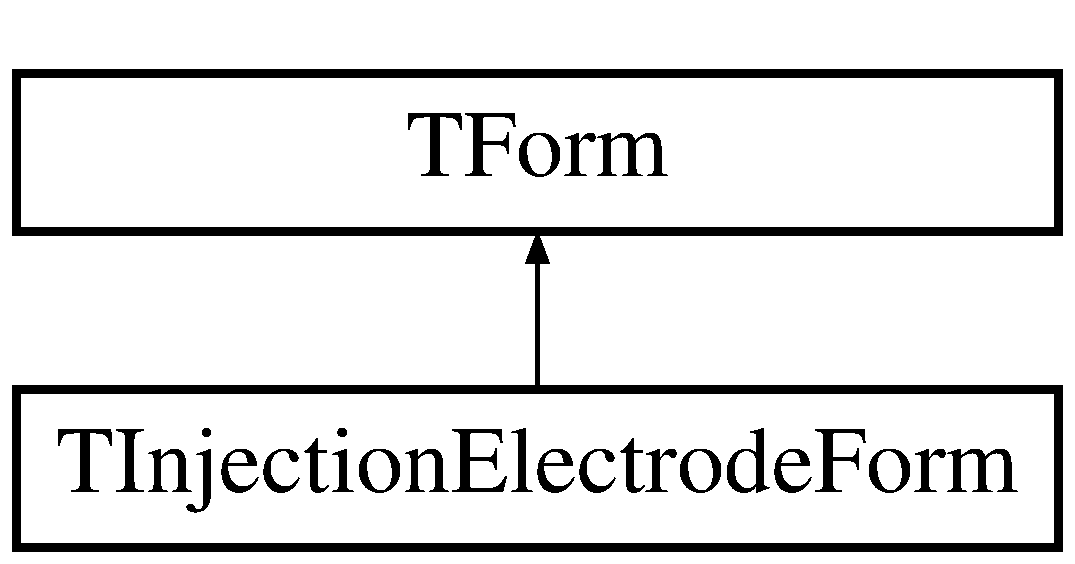
\includegraphics[height=2.000000cm]{class_t_injection_electrode_form}
\end{center}
\end{figure}
\subsection*{Public Member Functions}
\begin{DoxyCompactItemize}
\item 
\hypertarget{class_t_injection_electrode_form_ac01b7a316e160953c4bbab8d0390004a}{void \+\_\+\+\_\+fastcall {\bfseries Value\+List\+Editor1\+Key\+Press} (T\+Object $\ast$Sender, wchar\+\_\+t \&Key)}\label{class_t_injection_electrode_form_ac01b7a316e160953c4bbab8d0390004a}

\item 
\hypertarget{class_t_injection_electrode_form_a0305d33ca929f94292adffb076ee0706}{\+\_\+\+\_\+fastcall {\bfseries T\+Injection\+Electrode\+Form} (T\+Component $\ast$Owner)}\label{class_t_injection_electrode_form_a0305d33ca929f94292adffb076ee0706}

\end{DoxyCompactItemize}
\subsection*{Public Attributes}
\begin{DoxyCompactItemize}
\item 
\hypertarget{class_t_injection_electrode_form_aba3e4b0bff7fa065b9dccb57face3cd2}{T\+Label $\ast$ {\bfseries Label1}}\label{class_t_injection_electrode_form_aba3e4b0bff7fa065b9dccb57face3cd2}

\item 
\hypertarget{class_t_injection_electrode_form_a43494755a6902dd536d067f904fa8eeb}{T\+Value\+List\+Editor $\ast$ {\bfseries Value\+List\+Editor1}}\label{class_t_injection_electrode_form_a43494755a6902dd536d067f904fa8eeb}

\item 
\hypertarget{class_t_injection_electrode_form_a202b2414858cb3c1485cb11cce2b2433}{\hyperlink{class_t_injection_electrode}{T\+Injection\+Electrode} $\ast$ {\bfseries Inj\+Electrode}}\label{class_t_injection_electrode_form_a202b2414858cb3c1485cb11cce2b2433}

\end{DoxyCompactItemize}


\subsection{Detailed Description}
G\+U\+I Editor for \hyperlink{class_t_injection_electrode}{T\+Injection\+Electrode}. 

\begin{DoxyAuthor}{Author}
E. Brady Trexler $<$ebtrexler (at) gothamsci.\+com$>$, 2011 -\/ 2013 
\end{DoxyAuthor}


The documentation for this class was generated from the following files\+:\begin{DoxyCompactItemize}
\item 
G\+U\+I\+\_\+\+R\+T\+\_\+\+Edit\+\_\+\+Inj\+Electrode.\+h\item 
G\+U\+I\+\_\+\+R\+T\+\_\+\+Edit\+\_\+\+Inj\+Electrode.\+cpp\end{DoxyCompactItemize}

\hypertarget{class_t_model_base}{\section{T\+Model\+Base Class Reference}
\label{class_t_model_base}\index{T\+Model\+Base@{T\+Model\+Base}}
}
Inheritance diagram for T\+Model\+Base\+:\begin{figure}[H]
\begin{center}
\leavevmode
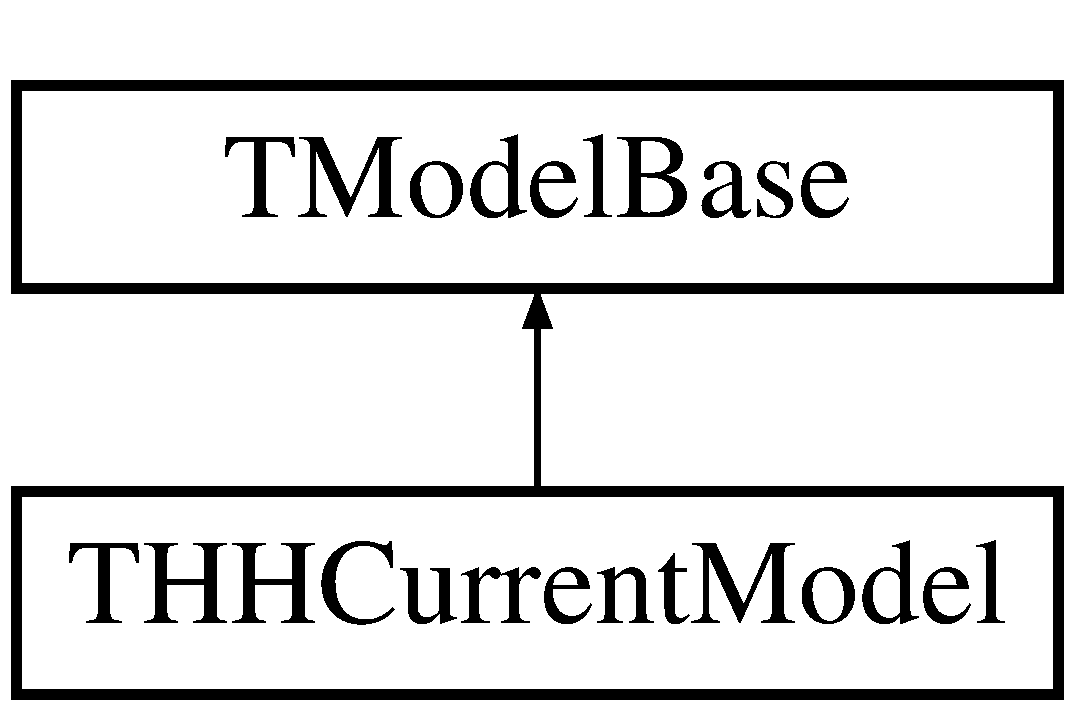
\includegraphics[height=2.000000cm]{class_t_model_base}
\end{center}
\end{figure}
\subsection*{Public Member Functions}
\begin{DoxyCompactItemize}
\item 
\hypertarget{class_t_model_base_aad916cbf9c170e09088b497bea71fd85}{virtual int \+\_\+\+\_\+fastcall {\bfseries Out\+Fit} ()=0}\label{class_t_model_base_aad916cbf9c170e09088b497bea71fd85}

\item 
\hypertarget{class_t_model_base_a43338827724d2585caadbd664adbf7fa}{virtual double \+\_\+\+\_\+fastcall {\bfseries Get\+Chi\+Sq} ()=0}\label{class_t_model_base_a43338827724d2585caadbd664adbf7fa}

\item 
\hypertarget{class_t_model_base_add4c311a969dbf5c2b1f1d5c4c72bb24}{virtual int \+\_\+\+\_\+fastcall {\bfseries fit\+Gen} (int $\ast$numdatapoints, int $\ast$numparms, double $\ast$parms, double $\ast$fvec, int $\ast$iflag)=0}\label{class_t_model_base_add4c311a969dbf5c2b1f1d5c4c72bb24}

\end{DoxyCompactItemize}
\subsection*{Public Attributes}
\begin{DoxyCompactItemize}
\item 
\hypertarget{class_t_model_base_a141a231d1206ee8f9ffcd3e63bfd89af}{int {\bfseries Num\+Data\+Points}}\label{class_t_model_base_a141a231d1206ee8f9ffcd3e63bfd89af}

\item 
\hypertarget{class_t_model_base_a8be201a23a96e6c9290fda2c2e1814da}{double {\bfseries Tol}}\label{class_t_model_base_a8be201a23a96e6c9290fda2c2e1814da}

\item 
\hypertarget{class_t_model_base_a2a1152e491c7a8daa9eb62ddacaccd00}{std\+::string {\bfseries Description}}\label{class_t_model_base_a2a1152e491c7a8daa9eb62ddacaccd00}

\item 
\hypertarget{class_t_model_base_a121d715cf9c4ed34beb058a9ac786984}{std\+::vector$<$ double $>$ {\bfseries Seed\+Params}}\label{class_t_model_base_a121d715cf9c4ed34beb058a9ac786984}

\item 
\hypertarget{class_t_model_base_a201dbd704caa57660bec39afc6437889}{std\+::vector$<$ double $>$ {\bfseries Fit\+Params}}\label{class_t_model_base_a201dbd704caa57660bec39afc6437889}

\item 
\hypertarget{class_t_model_base_a2f40d254d600d2974973a47ccd418521}{std\+::vector$<$ std\+::string $>$ {\bfseries Param\+Desc}}\label{class_t_model_base_a2f40d254d600d2974973a47ccd418521}

\item 
\hypertarget{class_t_model_base_a6c2c3425fcbb0c039761eebe7067d221}{std\+::vector$<$ int $>$ {\bfseries Do\+Fit}}\label{class_t_model_base_a6c2c3425fcbb0c039761eebe7067d221}

\item 
\hypertarget{class_t_model_base_a4b5f5e1aa456a05ccfcbb5162c1975b9}{int {\bfseries Num\+Params}}\label{class_t_model_base_a4b5f5e1aa456a05ccfcbb5162c1975b9}

\item 
\hypertarget{class_t_model_base_af5b576699d5814295b16078d3781a099}{int {\bfseries Num\+Calls}}\label{class_t_model_base_af5b576699d5814295b16078d3781a099}

\item 
\hypertarget{class_t_model_base_a2669507f1778e5a0cf34dc94385f5cea}{int {\bfseries Every\+Other}}\label{class_t_model_base_a2669507f1778e5a0cf34dc94385f5cea}

\end{DoxyCompactItemize}


The documentation for this class was generated from the following files\+:\begin{DoxyCompactItemize}
\item 
Fit\+\_\+\+Levenberg\+Maquardt.\+h\item 
Fit\+\_\+\+Levenberg\+Maquardt.\+cpp\end{DoxyCompactItemize}

\hypertarget{class_t_model_cell}{\section{T\+Model\+Cell Class Reference}
\label{class_t_model_cell}\index{T\+Model\+Cell@{T\+Model\+Cell}}
}


Implements a cell whose voltage is updated by numerical integration.  


Inheritance diagram for T\+Model\+Cell\+:\begin{figure}[H]
\begin{center}
\leavevmode
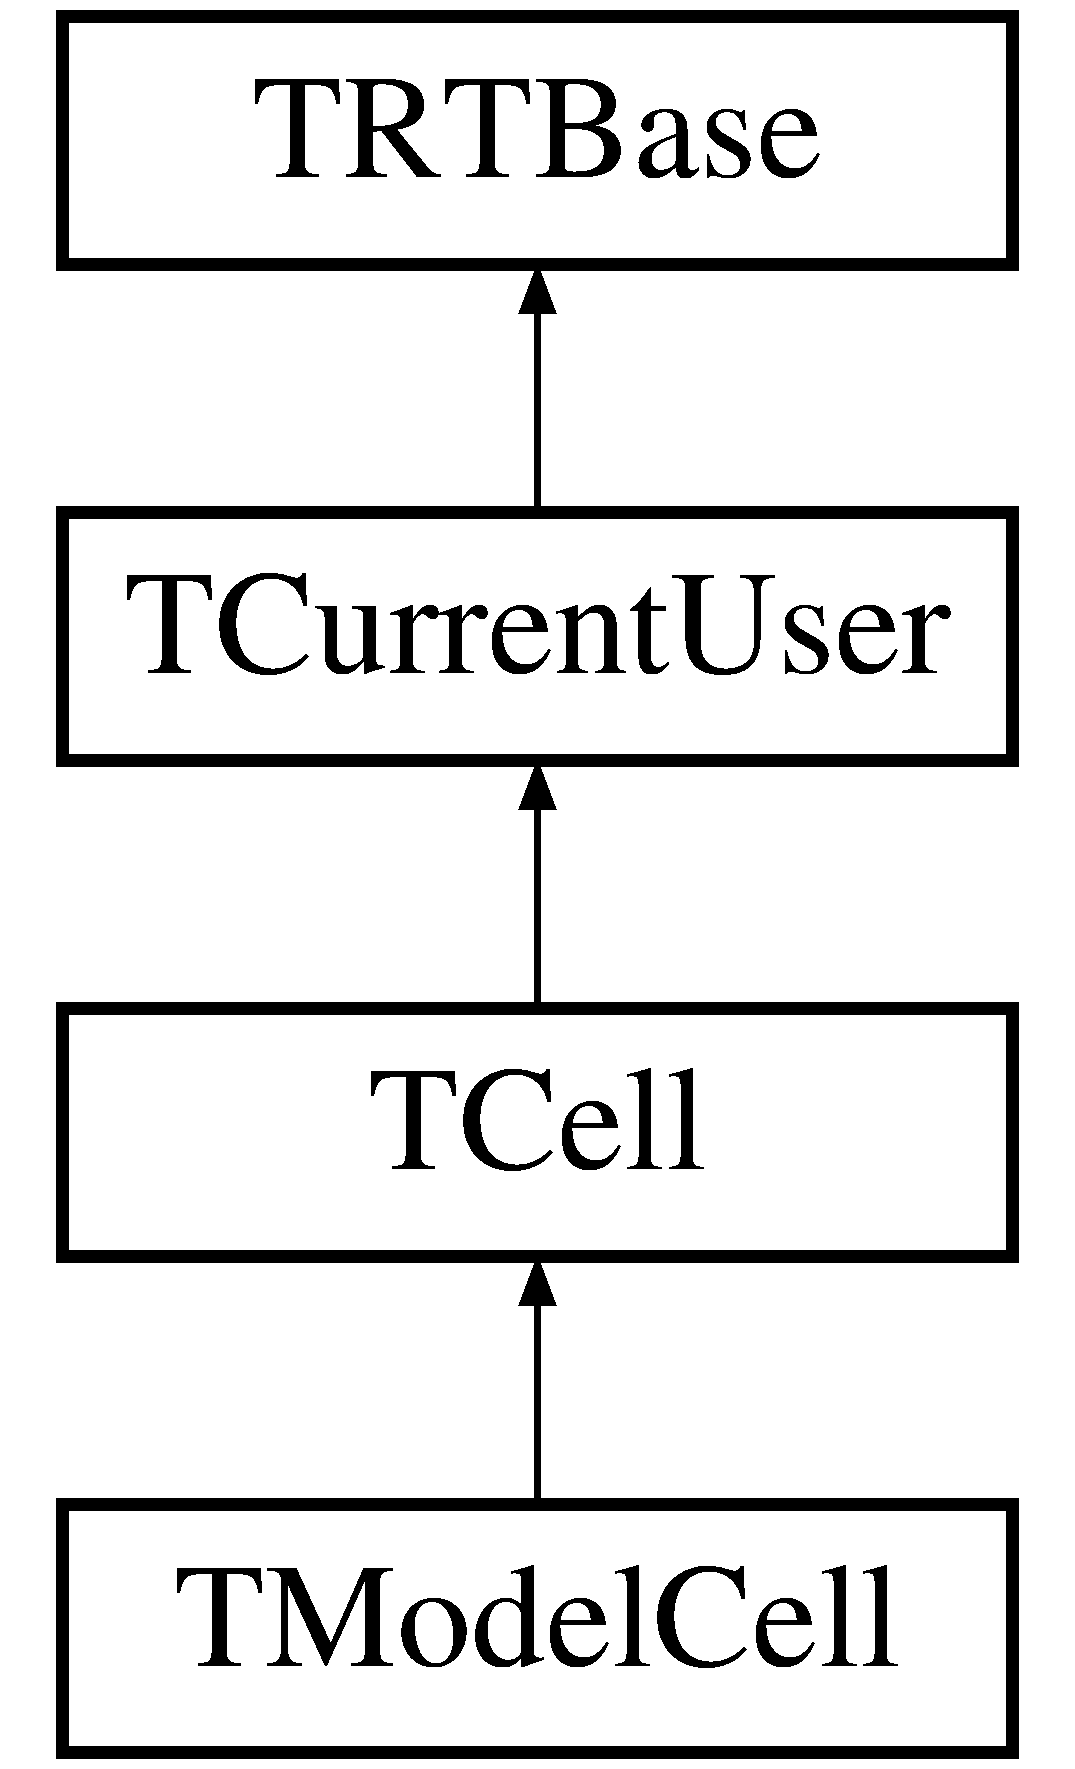
\includegraphics[height=4.000000cm]{class_t_model_cell}
\end{center}
\end{figure}
\subsection*{Public Member Functions}
\begin{DoxyCompactItemize}
\item 
\hypertarget{class_t_model_cell_ac81ddf570c5e202e118df93358b27346}{void \+\_\+\+\_\+fastcall \hyperlink{class_t_model_cell_ac81ddf570c5e202e118df93358b27346}{Populate\+Edit\+Form} ()}\label{class_t_model_cell_ac81ddf570c5e202e118df93358b27346}

\begin{DoxyCompactList}\small\item\em Interface for derived classes, called by G\+U\+I to update V\+C\+L form components. \end{DoxyCompactList}\item 
\hypertarget{class_t_model_cell_af0270c4542ef0650730894f4eeb18ddd}{bool \+\_\+\+\_\+fastcall \hyperlink{class_t_model_cell_af0270c4542ef0650730894f4eeb18ddd}{Validate\+Edit\+Form} ()}\label{class_t_model_cell_af0270c4542ef0650730894f4eeb18ddd}

\begin{DoxyCompactList}\small\item\em Interface for derived classes, called by G\+U\+I to read V\+C\+L form values. \end{DoxyCompactList}\item 
void $\ast$const \+\_\+\+\_\+fastcall \hyperlink{class_t_model_cell_af69daf6390baa3fc7ba7c11aa0d726ad}{Get\+Edit\+Form} ()
\item 
const std\+::wstring \&\+\_\+\+\_\+fastcall \hyperlink{class_t_model_cell_aaaffe113670920605dffda564b475ad0}{Class\+Key} () const 
\begin{DoxyCompactList}\small\item\em Returns string used to register class with factory. \end{DoxyCompactList}\item 
\hypertarget{class_t_model_cell_ad4ff3db085daa54b5aa2005fa5c87452}{\+\_\+\+\_\+fastcall \hyperlink{class_t_model_cell_ad4ff3db085daa54b5aa2005fa5c87452}{T\+Model\+Cell} ()}\label{class_t_model_cell_ad4ff3db085daa54b5aa2005fa5c87452}

\begin{DoxyCompactList}\small\item\em Default constructor. \end{DoxyCompactList}\item 
\hypertarget{class_t_model_cell_a7815944ffd27ce0c0d20f97bf1d4a668}{\+\_\+\+\_\+fastcall \hyperlink{class_t_model_cell_a7815944ffd27ce0c0d20f97bf1d4a668}{T\+Model\+Cell} (const std\+::wstring \&name)}\label{class_t_model_cell_a7815944ffd27ce0c0d20f97bf1d4a668}

\begin{DoxyCompactList}\small\item\em Specialized constructor. \end{DoxyCompactList}\item 
\hypertarget{class_t_model_cell_a6f5963a730ecb73442ef7c540eb07d58}{\+\_\+\+\_\+fastcall \hyperlink{class_t_model_cell_a6f5963a730ecb73442ef7c540eb07d58}{T\+Model\+Cell} (const \hyperlink{class_t_model_cell}{T\+Model\+Cell} \&source)}\label{class_t_model_cell_a6f5963a730ecb73442ef7c540eb07d58}

\begin{DoxyCompactList}\small\item\em Copy constructor. \end{DoxyCompactList}\item 
\hypertarget{class_t_model_cell_aec615232e0991a4b72930f68a0f0e831}{\hyperlink{class_t_model_cell}{T\+Model\+Cell} \& \hyperlink{class_t_model_cell_aec615232e0991a4b72930f68a0f0e831}{operator=} (const \hyperlink{class_t_model_cell}{T\+Model\+Cell} \&source)}\label{class_t_model_cell_aec615232e0991a4b72930f68a0f0e831}

\begin{DoxyCompactList}\small\item\em Overloaded assignment operator. \end{DoxyCompactList}\item 
\hypertarget{class_t_model_cell_a0e461d64396633fa3c5b898e4ea556fd}{virtual double \+\_\+\+\_\+fastcall \hyperlink{class_t_model_cell_a0e461d64396633fa3c5b898e4ea556fd}{Set\+Vm} (double \hyperlink{class_t_cell_afd81f2fd923ffbfa5ea7eda2c50693d1}{Vm})}\label{class_t_model_cell_a0e461d64396633fa3c5b898e4ea556fd}

\begin{DoxyCompactList}\small\item\em Sets membrane voltage -- must be overriden. \end{DoxyCompactList}\item 
\hypertarget{class_t_model_cell_ac87005aa33928e1206b60902e61531f7}{virtual double {\bfseries f} (double y)}\label{class_t_model_cell_ac87005aa33928e1206b60902e61531f7}

\item 
\hypertarget{class_t_model_cell_ab5bb6207de8a3ed08b7596407b34e36e}{virtual double {\bfseries rk4} (double y\+\_\+n, double step)}\label{class_t_model_cell_ab5bb6207de8a3ed08b7596407b34e36e}

\item 
\hypertarget{class_t_model_cell_af209cc096fc2b2da71d28e8a78ad0db2}{virtual double \+\_\+\+\_\+fastcall \hyperlink{class_t_model_cell_af209cc096fc2b2da71d28e8a78ad0db2}{Calc\+Vm} (double step)}\label{class_t_model_cell_af209cc096fc2b2da71d28e8a78ad0db2}

\begin{DoxyCompactList}\small\item\em Calculates membrane voltage -- must be overridden. \end{DoxyCompactList}\item 
\hypertarget{class_t_model_cell_a803808cc5f1c906df5d5b1b2d33bd3fa}{bool \+\_\+\+\_\+fastcall \hyperlink{class_t_model_cell_a803808cc5f1c906df5d5b1b2d33bd3fa}{Is\+Voltage\+Dependent} ()}\label{class_t_model_cell_a803808cc5f1c906df5d5b1b2d33bd3fa}

\begin{DoxyCompactList}\small\item\em Used to classify cell as biological (true) or other (false) \end{DoxyCompactList}\item 
\hypertarget{class_t_model_cell_a402870531adc0f74fe1785db3c3ee74f}{bool \+\_\+\+\_\+fastcall \hyperlink{class_t_model_cell_a402870531adc0f74fe1785db3c3ee74f}{Initialize} (bool Reset)}\label{class_t_model_cell_a402870531adc0f74fe1785db3c3ee74f}

\begin{DoxyCompactList}\small\item\em pure virtual function for resetting before networking run \end{DoxyCompactList}\item 
\hypertarget{class_t_model_cell_a2beab2b6327c27d8fc962f158959362c}{virtual const bool \+\_\+\+\_\+fastcall \hyperlink{class_t_model_cell_a2beab2b6327c27d8fc962f158959362c}{Accepts\+Currents} () const }\label{class_t_model_cell_a2beab2b6327c27d8fc962f158959362c}

\begin{DoxyCompactList}\small\item\em Informs caller whether can accept currents or not. \end{DoxyCompactList}\end{DoxyCompactItemize}
\subsection*{Protected Member Functions}
\begin{DoxyCompactItemize}
\item 
\hypertarget{class_t_model_cell_ada53cf8aa063c8b8f8db1eff8c9ddb67}{void const \+\_\+\+\_\+fastcall \hyperlink{class_t_model_cell_ada53cf8aa063c8b8f8db1eff8c9ddb67}{Write\+To\+Stream} (ostream \&stream) const }\label{class_t_model_cell_ada53cf8aa063c8b8f8db1eff8c9ddb67}

\begin{DoxyCompactList}\small\item\em Writes data members to a stream. \end{DoxyCompactList}\item 
\hypertarget{class_t_model_cell_a94252d562aa94352f259d2efa371c0b8}{void const \+\_\+\+\_\+fastcall \hyperlink{class_t_model_cell_a94252d562aa94352f259d2efa371c0b8}{Read\+From\+Stream} (istream \&stream)}\label{class_t_model_cell_a94252d562aa94352f259d2efa371c0b8}

\begin{DoxyCompactList}\small\item\em pure virtual function for derived classes to read from a stream \end{DoxyCompactList}\end{DoxyCompactItemize}
\subsection*{Friends}
\begin{DoxyCompactItemize}
\item 
\hypertarget{class_t_model_cell_ac98d07dd8f7b70e16ccb9a01abf56b9c}{class {\bfseries boost\+::serialization\+::access}}\label{class_t_model_cell_ac98d07dd8f7b70e16ccb9a01abf56b9c}

\end{DoxyCompactItemize}
\subsection*{Additional Inherited Members}


\subsection{Detailed Description}
Implements a cell whose voltage is updated by numerical integration. 

\hyperlink{class_t_model_cell_af209cc096fc2b2da71d28e8a78ad0db2}{Calc\+Vm()} method called to update membrane voltage. Then all \hyperlink{class_t_cell_ab65843b9b3021e0d2e614edb4ac1a18e}{Update()} is called so that intrinsic currents, synaptic currents, and electrode currents are calculated and summed.

\begin{DoxyAuthor}{Author}
E. Brady Trexler $<$ebtrexler (at) gothamsci.\+com$>$, 2011 -\/ 2013 
\end{DoxyAuthor}


\subsection{Member Function Documentation}
\hypertarget{class_t_model_cell_aaaffe113670920605dffda564b475ad0}{\index{T\+Model\+Cell@{T\+Model\+Cell}!Class\+Key@{Class\+Key}}
\index{Class\+Key@{Class\+Key}!T\+Model\+Cell@{T\+Model\+Cell}}
\subsubsection[{Class\+Key}]{\setlength{\rightskip}{0pt plus 5cm}const std\+::wstring\& \+\_\+\+\_\+fastcall T\+Model\+Cell\+::\+Class\+Key (
\begin{DoxyParamCaption}
{}
\end{DoxyParamCaption}
) const\hspace{0.3cm}{\ttfamily [inline]}, {\ttfamily [virtual]}}}\label{class_t_model_cell_aaaffe113670920605dffda564b475ad0}


Returns string used to register class with factory. 

Users of class factories must also tell the class the key they used when registering the class. See factory.\+h 

Implements \hyperlink{class_t_r_t_base_a6083fd510cbcb00faa85e5934fc3c18e}{T\+R\+T\+Base}.

\hypertarget{class_t_model_cell_af69daf6390baa3fc7ba7c11aa0d726ad}{\index{T\+Model\+Cell@{T\+Model\+Cell}!Get\+Edit\+Form@{Get\+Edit\+Form}}
\index{Get\+Edit\+Form@{Get\+Edit\+Form}!T\+Model\+Cell@{T\+Model\+Cell}}
\subsubsection[{Get\+Edit\+Form}]{\setlength{\rightskip}{0pt plus 5cm}void$\ast$ const \+\_\+\+\_\+fastcall T\+Model\+Cell\+::\+Get\+Edit\+Form (
\begin{DoxyParamCaption}
{}
\end{DoxyParamCaption}
)\hspace{0.3cm}{\ttfamily [inline]}, {\ttfamily [virtual]}}}\label{class_t_model_cell_af69daf6390baa3fc7ba7c11aa0d726ad}
Interface for derived classes, returns pointer to G\+U\+I object for editing members. Callers must cast pointer to the correct object. 

Implements \hyperlink{class_t_r_t_base_ab83e520005e20ee71f98f3e85e1ee6d4}{T\+R\+T\+Base}.



The documentation for this class was generated from the following file\+:\begin{DoxyCompactItemize}
\item 
G\+U\+I\+\_\+\+R\+T\+\_\+\+Edit\+\_\+\+Model\+Cell.\+cpp\end{DoxyCompactItemize}

\hypertarget{class_t_model_cell_form}{\section{T\+Model\+Cell\+Form Class Reference}
\label{class_t_model_cell_form}\index{T\+Model\+Cell\+Form@{T\+Model\+Cell\+Form}}
}


G\+U\+I editor for \hyperlink{class_t_model_cell}{T\+Model\+Cell}.  




{\ttfamily \#include $<$G\+U\+I\+\_\+\+R\+T\+\_\+\+Edit\+\_\+\+Model\+Cell.\+h$>$}

Inheritance diagram for T\+Model\+Cell\+Form\+:\begin{figure}[H]
\begin{center}
\leavevmode
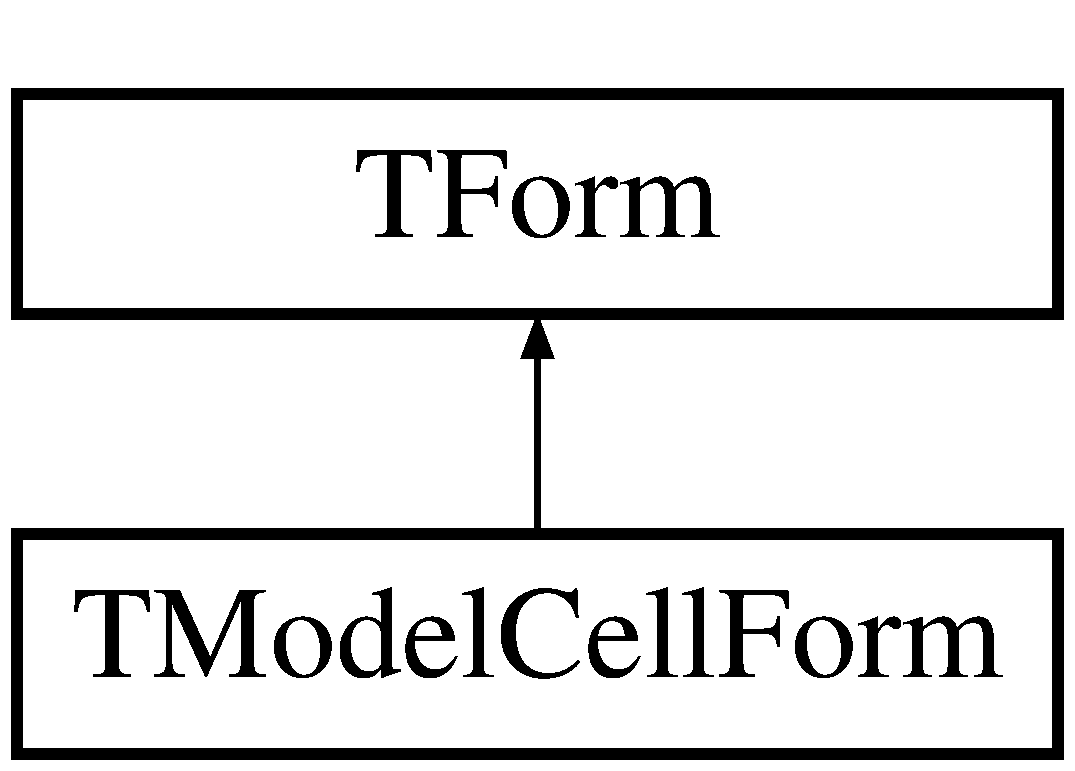
\includegraphics[height=2.000000cm]{class_t_model_cell_form}
\end{center}
\end{figure}
\subsection*{Public Member Functions}
\begin{DoxyCompactItemize}
\item 
\hypertarget{class_t_model_cell_form_a93464aa737f44f3f044bc9f58de01b6f}{void \+\_\+\+\_\+fastcall {\bfseries Edit\+Key\+Press} (T\+Object $\ast$Sender, wchar\+\_\+t \&Key)}\label{class_t_model_cell_form_a93464aa737f44f3f044bc9f58de01b6f}

\item 
\hypertarget{class_t_model_cell_form_a8126b0caa81411a38b99b1b1bbf66533}{\+\_\+\+\_\+fastcall {\bfseries T\+Model\+Cell\+Form} (T\+Component $\ast$Owner)}\label{class_t_model_cell_form_a8126b0caa81411a38b99b1b1bbf66533}

\end{DoxyCompactItemize}
\subsection*{Public Attributes}
\begin{DoxyCompactItemize}
\item 
\hypertarget{class_t_model_cell_form_a7d221872898b803eb8a5aa4ecb815a40}{T\+Label $\ast$ {\bfseries Label1}}\label{class_t_model_cell_form_a7d221872898b803eb8a5aa4ecb815a40}

\item 
\hypertarget{class_t_model_cell_form_a8c09f791520b94540028fb52a6508cd3}{T\+Label $\ast$ {\bfseries Label2}}\label{class_t_model_cell_form_a8c09f791520b94540028fb52a6508cd3}

\item 
\hypertarget{class_t_model_cell_form_a066f5256e98efe16013f2fb49c365e92}{T\+Edit $\ast$ {\bfseries Capacitance\+Edit}}\label{class_t_model_cell_form_a066f5256e98efe16013f2fb49c365e92}

\item 
\hypertarget{class_t_model_cell_form_a73ba468f4aac61eb23832b0916632eef}{T\+Label $\ast$ {\bfseries Label3}}\label{class_t_model_cell_form_a73ba468f4aac61eb23832b0916632eef}

\item 
\hypertarget{class_t_model_cell_form_af64cc01398fdad784c2a2506fc8ad87f}{T\+Edit $\ast$ {\bfseries Initial\+Vm\+Edit}}\label{class_t_model_cell_form_af64cc01398fdad784c2a2506fc8ad87f}

\item 
\hypertarget{class_t_model_cell_form_a15498a327c0a22d3596b497189987070}{T\+Label $\ast$ {\bfseries Label4}}\label{class_t_model_cell_form_a15498a327c0a22d3596b497189987070}

\item 
\hypertarget{class_t_model_cell_form_ac696daa160db91afdea1de76a3e5057a}{\hyperlink{class_t_model_cell}{T\+Model\+Cell} $\ast$ {\bfseries Model\+Cell}}\label{class_t_model_cell_form_ac696daa160db91afdea1de76a3e5057a}

\end{DoxyCompactItemize}


\subsection{Detailed Description}
G\+U\+I editor for \hyperlink{class_t_model_cell}{T\+Model\+Cell}. 

\begin{DoxyAuthor}{Author}
E. Brady Trexler $<$ebtrexler (at) gothamsci.\+com$>$, 2011 -\/ 2013 
\end{DoxyAuthor}


The documentation for this class was generated from the following files\+:\begin{DoxyCompactItemize}
\item 
G\+U\+I\+\_\+\+R\+T\+\_\+\+Edit\+\_\+\+Model\+Cell.\+h\item 
G\+U\+I\+\_\+\+R\+T\+\_\+\+Edit\+\_\+\+Model\+Cell.\+cpp\end{DoxyCompactItemize}

\hypertarget{class_t_network}{\section{T\+Network Class Reference}
\label{class_t_network}\index{T\+Network@{T\+Network}}
}


Complete class that handles network creation, editing and running of simulations.  




{\ttfamily \#include $<$R\+T\+\_\+\+Network.\+h$>$}

Inheritance diagram for T\+Network\+:\begin{figure}[H]
\begin{center}
\leavevmode
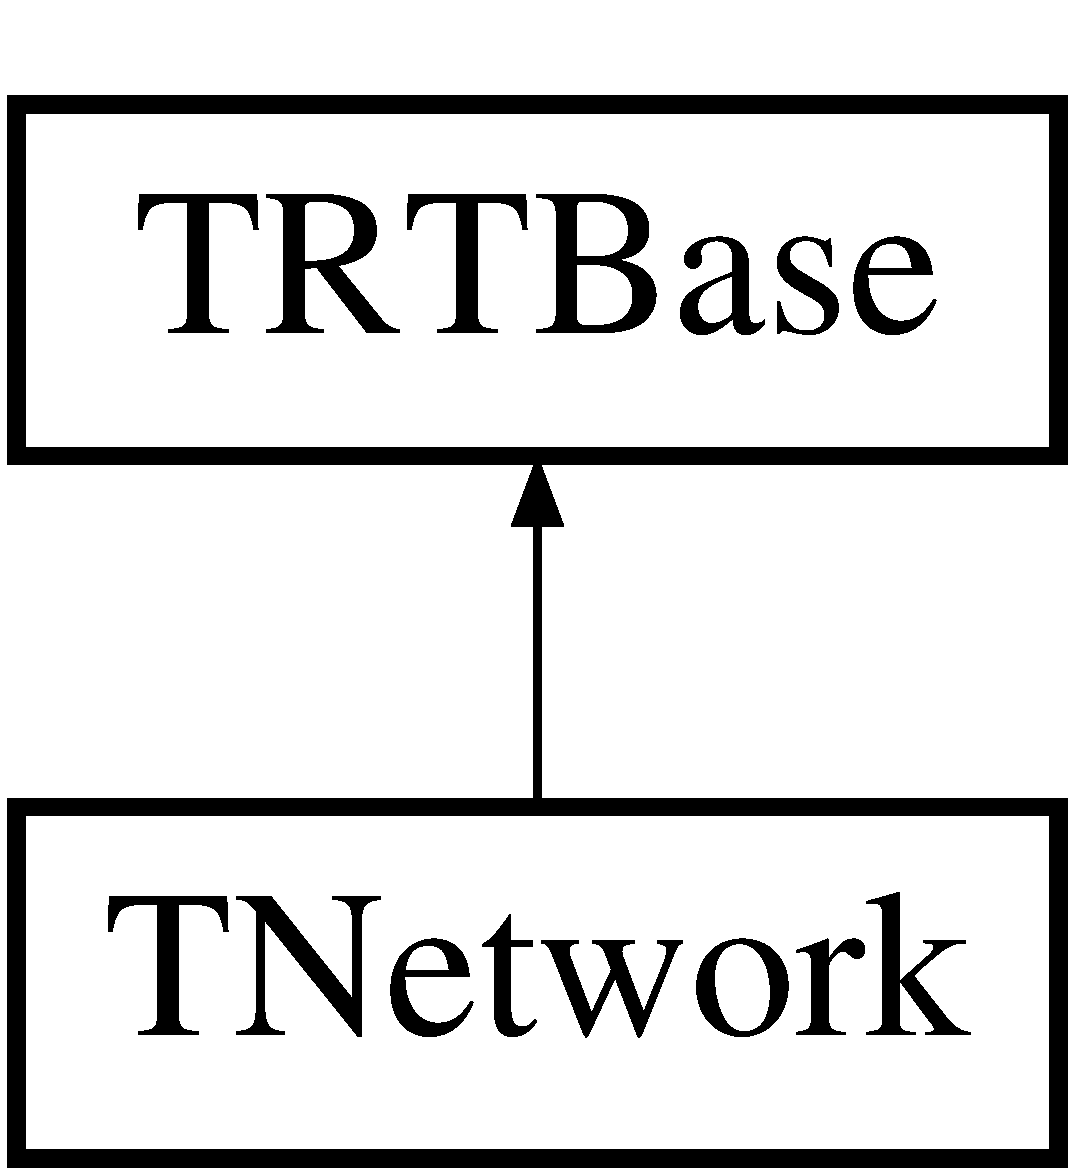
\includegraphics[height=2.000000cm]{class_t_network}
\end{center}
\end{figure}
\subsection*{Public Member Functions}
\begin{DoxyCompactItemize}
\item 
\hypertarget{class_t_network_ad526c42cca14e656a0d84134d03231b6}{virtual const T\+Cells\+Map \&\+\_\+\+\_\+fastcall \hyperlink{class_t_network_ad526c42cca14e656a0d84134d03231b6}{Get\+Cells} ()}\label{class_t_network_ad526c42cca14e656a0d84134d03231b6}

\begin{DoxyCompactList}\small\item\em Returns reference to Cells map. \end{DoxyCompactList}\item 
\hypertarget{class_t_network_ad4e242b97eb3385e9fd24d9dc2885970}{virtual const T\+Synapses\+Map \\*
\&\+\_\+\+\_\+fastcall \hyperlink{class_t_network_ad4e242b97eb3385e9fd24d9dc2885970}{Get\+Synapses} ()}\label{class_t_network_ad4e242b97eb3385e9fd24d9dc2885970}

\begin{DoxyCompactList}\small\item\em Returns reference to Synapses map. \end{DoxyCompactList}\item 
\hypertarget{class_t_network_a18855029644af07d17bfcb7b39b8045b}{virtual const T\+Electrodes\+Map \\*
\&\+\_\+\+\_\+fastcall \hyperlink{class_t_network_a18855029644af07d17bfcb7b39b8045b}{Get\+Electrodes} ()}\label{class_t_network_a18855029644af07d17bfcb7b39b8045b}

\begin{DoxyCompactList}\small\item\em Returns reference to Electrodes map. \end{DoxyCompactList}\item 
\hypertarget{class_t_network_ae34128013b8bb9949c3f83c496894042}{virtual const double \+\_\+\+\_\+fastcall \hyperlink{class_t_network_ae34128013b8bb9949c3f83c496894042}{Get\+Max\+R\+K4\+Timestep} () const }\label{class_t_network_ae34128013b8bb9949c3f83c496894042}

\begin{DoxyCompactList}\small\item\em Runge-\/\+Kutta time step getter method. \end{DoxyCompactList}\item 
\hypertarget{class_t_network_ad76213030f30e7ad850cc0c37c84a2da}{virtual void \+\_\+\+\_\+fastcall \hyperlink{class_t_network_ad76213030f30e7ad850cc0c37c84a2da}{Set\+Max\+R\+K4\+Timestep} (double rk4step)}\label{class_t_network_ad76213030f30e7ad850cc0c37c84a2da}

\begin{DoxyCompactList}\small\item\em Runge-\/\+Kutta time step setter method. \end{DoxyCompactList}\item 
\hypertarget{class_t_network_a26507c4e11b3c5caf36625f6d5fc92e7}{virtual const double \+\_\+\+\_\+fastcall {\bfseries Elapsed\+Time} () const }\label{class_t_network_a26507c4e11b3c5caf36625f6d5fc92e7}

\item 
\hypertarget{class_t_network_ae89373d91a4136126cb871fd4c541cf0}{const bool \+\_\+\+\_\+fastcall \hyperlink{class_t_network_ae89373d91a4136126cb871fd4c541cf0}{Is\+Param\+Logging\+Enabled} () const }\label{class_t_network_ae89373d91a4136126cb871fd4c541cf0}

\begin{DoxyCompactList}\small\item\em Determines if parameter logging to a stream is enabled. \end{DoxyCompactList}\item 
\hypertarget{class_t_network_a60a220f1d272aec26152ffe4b80a3c64}{void \+\_\+\+\_\+fastcall \hyperlink{class_t_network_a60a220f1d272aec26152ffe4b80a3c64}{Set\+Param\+Logging\+Enabled} (bool enabled)}\label{class_t_network_a60a220f1d272aec26152ffe4b80a3c64}

\begin{DoxyCompactList}\small\item\em Determines if parameter logging to a stream is enabled. \end{DoxyCompactList}\item 
virtual void \+\_\+\+\_\+fastcall \hyperlink{class_t_network_a39e0717cf1e0d0134053871a7199376f}{Write\+Param\+Logging\+Header} ()
\begin{DoxyCompactList}\small\item\em Writes tab-\/delimited column names for paramter logging. \end{DoxyCompactList}\item 
\hypertarget{class_t_network_ac4785621fe020479391e6279a388af22}{virtual void \+\_\+\+\_\+fastcall \hyperlink{class_t_network_ac4785621fe020479391e6279a388af22}{Write\+Header\+For\+Cell\+Currents} (\hyperlink{class_t_cell}{T\+Cell} $\ast$cell)}\label{class_t_network_ac4785621fe020479391e6279a388af22}

\begin{DoxyCompactList}\small\item\em Writes headers for intrinsic and synaptic currents for each cell. \end{DoxyCompactList}\item 
\hypertarget{class_t_network_ac47a2d67ec939b6e0a898cae11af24aa}{virtual \hyperlink{class_t_data_logger}{T\+Data\+Logger} \&\+\_\+\+\_\+fastcall \hyperlink{class_t_network_ac47a2d67ec939b6e0a898cae11af24aa}{Get\+Param\+Logger} ()}\label{class_t_network_ac47a2d67ec939b6e0a898cae11af24aa}

\begin{DoxyCompactList}\small\item\em Output stream reference for logging variables getter method. \end{DoxyCompactList}\item 
\hypertarget{class_t_network_a4fe50c91d6a645e98132d1b616f63e34}{virtual void \+\_\+\+\_\+fastcall \hyperlink{class_t_network_a4fe50c91d6a645e98132d1b616f63e34}{Close\+Logging\+Stream} (const wchar\+\_\+t $\ast$filename)}\label{class_t_network_a4fe50c91d6a645e98132d1b616f63e34}

\begin{DoxyCompactList}\small\item\em Terminate logging. \end{DoxyCompactList}\item 
virtual \hyperlink{class_t_cell}{T\+Cell} $\ast$\+\_\+\+\_\+fastcall \hyperlink{class_t_network_aa6bd65ef73301e258fcb0a18f62aed65}{Add\+Cell\+To\+Net} (const std\+::wstring \&Cell\+Type, const std\+::wstring \&Cell\+Name, int X=0, int Y=0)
\begin{DoxyCompactList}\small\item\em Adds cell to network. \end{DoxyCompactList}\item 
virtual void \+\_\+\+\_\+fastcall \hyperlink{class_t_network_ad59490c229da774a859256f4c8152c3d}{Remove\+Cell\+From\+Net} (const std\+::wstring \&Cell\+Name)
\begin{DoxyCompactList}\small\item\em Removes cell from network. \end{DoxyCompactList}\item 
virtual void \+\_\+\+\_\+fastcall \hyperlink{class_t_network_ae2809d4ca770c3ef89533ff911219d25}{Set\+Cell\+Active\+State} (const std\+::wstring \&Cell\+Name, bool Active)
\begin{DoxyCompactList}\small\item\em Determines whether cell is included in calculations. \end{DoxyCompactList}\item 
virtual void \+\_\+\+\_\+fastcall \hyperlink{class_t_network_ad48a93ee8b8a5fc54afefcf1efba8c2c}{Rename\+Cell} (const std\+::wstring \&oldname, const std\+::wstring \&newname)
\begin{DoxyCompactList}\small\item\em Rename the cell. \end{DoxyCompactList}\item 
virtual void \+\_\+\+\_\+fastcall \hyperlink{class_t_network_ad7e77fdd48eef933de854aa4ea33e153}{Copy\+Currents\+From\+Cell} (const std\+::wstring \&fromname, const std\+::vector$<$ std\+::wstring $>$ tonames, bool Clear\+And\+Replace)
\begin{DoxyCompactList}\small\item\em Copy currents from one cell to one or more other cells. \end{DoxyCompactList}\item 
virtual \hyperlink{class_t_synapse}{T\+Synapse} $\ast$\+\_\+\+\_\+fastcall \hyperlink{class_t_network_ae0c23d5e84b2843a431584c01f64675b}{Add\+Synapse\+Between\+Cells} (const std\+::wstring \&Synapse\+Type, const std\+::wstring \&Synapse\+Name, const std\+::wstring \&Pre\+Cell\+Name, const std\+::wstring \&Post\+Cell\+Name, int X=0, int Y=0)
\begin{DoxyCompactList}\small\item\em Adds synapse to network between two cells. \end{DoxyCompactList}\item 
virtual void \+\_\+\+\_\+fastcall \hyperlink{class_t_network_ad9715f79cef5f979183157f03b974141}{Remove\+Synapse\+From\+Net} (const std\+::wstring \&Synapse\+Name)
\begin{DoxyCompactList}\small\item\em Removes synapse from network and disconnects two cells. \end{DoxyCompactList}\item 
virtual void \+\_\+\+\_\+fastcall \hyperlink{class_t_network_a22afbf4ddfc2298708e49fc6b6cc078a}{Set\+Synapse\+Active\+State} (const std\+::wstring \&Synapse\+Name, bool Active)
\begin{DoxyCompactList}\small\item\em Determines whether synapse is included in calculations. \end{DoxyCompactList}\item 
virtual void \+\_\+\+\_\+fastcall \hyperlink{class_t_network_afc3273cd3400c77d167887f9f344295c}{Rename\+Synapse} (const std\+::wstring \&oldname, const std\+::wstring \&newname)
\begin{DoxyCompactList}\small\item\em Rename the synapse. \end{DoxyCompactList}\item 
virtual \hyperlink{class_t_electrode}{T\+Electrode} $\ast$\+\_\+\+\_\+fastcall \hyperlink{class_t_network_ab312ec35a227f70119bf87eaad64ed7f}{Add\+Electrode\+To\+Cell} (const std\+::wstring \&Electrode\+Type, const std\+::wstring \&Electrode\+Name, const std\+::wstring \&Cell\+Name, int X=0, int Y=0)
\begin{DoxyCompactList}\small\item\em Adds electrode to a cell in the network. \end{DoxyCompactList}\item 
virtual void \+\_\+\+\_\+fastcall \hyperlink{class_t_network_a03936ad02ae65bdd73645b2e22c5b796}{Remove\+Electrode\+From\+Net} (const std\+::wstring \&Electrode\+Name)
\begin{DoxyCompactList}\small\item\em Removes electrode from network and its cell. \end{DoxyCompactList}\item 
virtual void \+\_\+\+\_\+fastcall \hyperlink{class_t_network_a509f7d39290fa7c82e613d5aae1498ce}{Set\+Electrode\+Active\+State} (const std\+::wstring \&Electrode\+Name, bool Active)
\begin{DoxyCompactList}\small\item\em Determines whether electrode is included in calculations. \end{DoxyCompactList}\item 
virtual void \+\_\+\+\_\+fastcall \hyperlink{class_t_network_a36ac85343172b38901261fe9ca0ede7e}{Rename\+Electrode} (const std\+::wstring \&oldname, const std\+::wstring \&newname)
\begin{DoxyCompactList}\small\item\em Rename the electrode. \end{DoxyCompactList}\item 
virtual \hyperlink{class_t_current}{T\+Current} $\ast$\+\_\+\+\_\+fastcall \hyperlink{class_t_network_afcb6c9ba3cea871b214cac5271776f03}{Add\+Current\+To\+Synapse} (const std\+::wstring \&Synapse\+Name, const std\+::wstring \&Current\+Type, const std\+::wstring \&Current\+Name, const std\+::wstring \&Cell\+Name)
\begin{DoxyCompactList}\small\item\em Adds current to a synapse in the network. \end{DoxyCompactList}\item 
virtual void \+\_\+\+\_\+fastcall \hyperlink{class_t_network_aee6565f15d005fa3daccaefe215b0946}{Remove\+Current\+From\+Synapse} (const std\+::wstring \&Current\+Name, const std\+::wstring \&Synapse\+Name)
\begin{DoxyCompactList}\small\item\em Removes current from synapse. \end{DoxyCompactList}\item 
virtual \hyperlink{class_t_current}{T\+Current} $\ast$\+\_\+\+\_\+fastcall \hyperlink{class_t_network_afd4e1483f03749ff479b3b5edfd94079}{Add\+Current\+To\+Cell} (const std\+::wstring \&Current\+Type, const std\+::wstring \&Current\+Name, const std\+::wstring \&Cell\+Name)
\begin{DoxyCompactList}\small\item\em Adds current to a cell in the network. \end{DoxyCompactList}\item 
virtual void \+\_\+\+\_\+fastcall \hyperlink{class_t_network_abfb4a743781ec3669a16404f5e4c3a35}{Remove\+Current\+From\+Cell} (const std\+::wstring \&Current\+Name, const std\+::wstring \&Cell\+Name)
\begin{DoxyCompactList}\small\item\em Removes current from cell. \end{DoxyCompactList}\item 
virtual void \+\_\+\+\_\+fastcall \hyperlink{class_t_network_ad1aaaa8e2b7afbe01087ece54b19e0ad}{Set\+Current\+Active\+State} (const std\+::wstring \&Current\+Name, bool Active)
\begin{DoxyCompactList}\small\item\em Determines whether current is included in calculations. \end{DoxyCompactList}\item 
virtual void \+\_\+\+\_\+fastcall \hyperlink{class_t_network_a435e422bce53a3e9dfb38271710aed4c}{Rename\+Current} (const std\+::wstring \&oldname, const std\+::wstring \&newname)
\begin{DoxyCompactList}\small\item\em Rename the current. \end{DoxyCompactList}\item 
virtual std\+::wstring \+\_\+\+\_\+fastcall \hyperlink{class_t_network_af2cad16d184fa37acbe7355ee00b384d}{Cell\+Grid\+Hit\+Test} (const int X, const int Y, int tol=0)
\begin{DoxyCompactList}\small\item\em G\+U\+I friendly function that determines the proximity of a position to a cell. \end{DoxyCompactList}\item 
\hypertarget{class_t_network_ac996464919d49a5aa5ec510369aab2be}{\+\_\+\+\_\+fastcall \hyperlink{class_t_network_ac996464919d49a5aa5ec510369aab2be}{T\+Network} ()}\label{class_t_network_ac996464919d49a5aa5ec510369aab2be}

\begin{DoxyCompactList}\small\item\em Default constructor. \end{DoxyCompactList}\item 
\hypertarget{class_t_network_a93f797373ab74025b7dea0d5c3568176}{\+\_\+\+\_\+fastcall \hyperlink{class_t_network_a93f797373ab74025b7dea0d5c3568176}{T\+Network} (const std\+::wstring \&name)}\label{class_t_network_a93f797373ab74025b7dea0d5c3568176}

\begin{DoxyCompactList}\small\item\em Specialized constructor. \end{DoxyCompactList}\item 
virtual double $\ast$\+\_\+\+\_\+fastcall \hyperlink{class_t_network_aa9ec65dcbbdad1ad67eaef33838a49c7}{Update} (double step, double $\ast$Vm\+\_\+in, double $\ast$Vm\+\_\+out, double $\ast$I\+\_\+n\+A)
\begin{DoxyCompactList}\small\item\em Updates the entire network -- called from D\+A\+Q classes. \end{DoxyCompactList}\item 
virtual \hyperlink{struct_net_description_struct}{Net\+Description\+Struct} \\*
\+\_\+\+\_\+fastcall \hyperlink{class_t_network_af0569ed2e0ecd9946996a030034510a3}{Describe\+Network} ()
\begin{DoxyCompactList}\small\item\em G\+U\+I or D\+A\+Q classes must call Describe\+Network before starting a run. \end{DoxyCompactList}\item 
\hypertarget{class_t_network_a2488896641ad4ceba1288ac86d0c6477}{virtual bool \+\_\+\+\_\+fastcall \hyperlink{class_t_network_a2488896641ad4ceba1288ac86d0c6477}{Initialize} (bool Reset)}\label{class_t_network_a2488896641ad4ceba1288ac86d0c6477}

\begin{DoxyCompactList}\small\item\em pure virtual function for resetting before networking run \end{DoxyCompactList}\item 
virtual const std\+::wstring \\*
\&\+\_\+\+\_\+fastcall \hyperlink{class_t_network_a9af68c6c12402bf185c1de44bab29a17}{Class\+Key} () const 
\begin{DoxyCompactList}\small\item\em Returns string used to register class with factory. \end{DoxyCompactList}\end{DoxyCompactItemize}
\subsection*{Friends}
\begin{DoxyCompactItemize}
\item 
\hypertarget{class_t_network_ac98d07dd8f7b70e16ccb9a01abf56b9c}{class \hyperlink{class_t_network_ac98d07dd8f7b70e16ccb9a01abf56b9c}{boost\+::serialization\+::access}}\label{class_t_network_ac98d07dd8f7b70e16ccb9a01abf56b9c}

\begin{DoxyCompactList}\small\item\em Required for serialization and saving networks to disk. \end{DoxyCompactList}\end{DoxyCompactItemize}
\subsection*{Additional Inherited Members}


\subsection{Detailed Description}
Complete class that handles network creation, editing and running of simulations. 

The \hyperlink{class_t_network}{T\+Network} class handles creation of objects. The relationships between objects are set in their constructors. Call the \hyperlink{class_t_network_aa9ec65dcbbdad1ad67eaef33838a49c7}{T\+Network\+::\+Update} function as it handles updating of child objects.

\hyperlink{class_t_network}{T\+Network} provides methods for accessing all children by their Name member. User interfaces should make use of this search ability.

There should be no need to derive from this class. It is self contained and ready to go.

\begin{DoxyAuthor}{Author}
E. Brady Trexler $<$ebtrexler (at) gothamsci.\+com$>$, 2011 -\/ 2013 
\end{DoxyAuthor}


\subsection{Member Function Documentation}
\hypertarget{class_t_network_aa6bd65ef73301e258fcb0a18f62aed65}{\index{T\+Network@{T\+Network}!Add\+Cell\+To\+Net@{Add\+Cell\+To\+Net}}
\index{Add\+Cell\+To\+Net@{Add\+Cell\+To\+Net}!T\+Network@{T\+Network}}
\subsubsection[{Add\+Cell\+To\+Net}]{\setlength{\rightskip}{0pt plus 5cm}{\bf T\+Cell} $\ast$\+\_\+\+\_\+fastcall T\+Network\+::\+Add\+Cell\+To\+Net (
\begin{DoxyParamCaption}
\item[{const std\+::wstring \&}]{Cell\+Type, }
\item[{const std\+::wstring \&}]{Cell\+Name, }
\item[{int}]{X = {\ttfamily 0}, }
\item[{int}]{Y = {\ttfamily 0}}
\end{DoxyParamCaption}
)\hspace{0.3cm}{\ttfamily [virtual]}}}\label{class_t_network_aa6bd65ef73301e258fcb0a18f62aed65}


Adds cell to network. 


\begin{DoxyParams}{Parameters}
{\em Cell\+Type} & is the C++ class type to add, derived from \hyperlink{class_t_cell}{T\+Cell} \\
\hline
{\em Cell\+Name} & is the unique name of the cell \\
\hline
{\em X} & is the distance of G\+U\+I representation from the left \\
\hline
{\em Y} & is the distance of G\+U\+I representation from the top \\
\hline
\end{DoxyParams}
\hypertarget{class_t_network_afd4e1483f03749ff479b3b5edfd94079}{\index{T\+Network@{T\+Network}!Add\+Current\+To\+Cell@{Add\+Current\+To\+Cell}}
\index{Add\+Current\+To\+Cell@{Add\+Current\+To\+Cell}!T\+Network@{T\+Network}}
\subsubsection[{Add\+Current\+To\+Cell}]{\setlength{\rightskip}{0pt plus 5cm}{\bf T\+Current} $\ast$\+\_\+\+\_\+fastcall T\+Network\+::\+Add\+Current\+To\+Cell (
\begin{DoxyParamCaption}
\item[{const std\+::wstring \&}]{Current\+Type, }
\item[{const std\+::wstring \&}]{Current\+Name, }
\item[{const std\+::wstring \&}]{Cell\+Name}
\end{DoxyParamCaption}
)\hspace{0.3cm}{\ttfamily [virtual]}}}\label{class_t_network_afd4e1483f03749ff479b3b5edfd94079}


Adds current to a cell in the network. 


\begin{DoxyParams}{Parameters}
{\em Current\+Type} & is the C++ class type to add, derived from \hyperlink{class_t_current}{T\+Current} \\
\hline
{\em Current\+Name} & is the unique name of the current \\
\hline
{\em Cell\+Name} & is cell to which current is applied \\
\hline
\end{DoxyParams}
\hypertarget{class_t_network_afcb6c9ba3cea871b214cac5271776f03}{\index{T\+Network@{T\+Network}!Add\+Current\+To\+Synapse@{Add\+Current\+To\+Synapse}}
\index{Add\+Current\+To\+Synapse@{Add\+Current\+To\+Synapse}!T\+Network@{T\+Network}}
\subsubsection[{Add\+Current\+To\+Synapse}]{\setlength{\rightskip}{0pt plus 5cm}{\bf T\+Current} $\ast$\+\_\+\+\_\+fastcall T\+Network\+::\+Add\+Current\+To\+Synapse (
\begin{DoxyParamCaption}
\item[{const std\+::wstring \&}]{Synapse\+Name, }
\item[{const std\+::wstring \&}]{Current\+Type, }
\item[{const std\+::wstring \&}]{Current\+Name, }
\item[{const std\+::wstring \&}]{Cell\+Name}
\end{DoxyParamCaption}
)\hspace{0.3cm}{\ttfamily [virtual]}}}\label{class_t_network_afcb6c9ba3cea871b214cac5271776f03}


Adds current to a synapse in the network. 


\begin{DoxyParams}{Parameters}
{\em Synapse\+Name} & is the unique name of the synapse \\
\hline
{\em Current\+Type} & is the C++ class type to add, derived from \hyperlink{class_t_current}{T\+Current} \\
\hline
{\em Current\+Name} & is the unique name of the current \\
\hline
{\em Cell\+Name} & is cell to which current is applied, either the pre-\/ or postsynaptic cell of the synapse \\
\hline
\end{DoxyParams}
\hypertarget{class_t_network_ab312ec35a227f70119bf87eaad64ed7f}{\index{T\+Network@{T\+Network}!Add\+Electrode\+To\+Cell@{Add\+Electrode\+To\+Cell}}
\index{Add\+Electrode\+To\+Cell@{Add\+Electrode\+To\+Cell}!T\+Network@{T\+Network}}
\subsubsection[{Add\+Electrode\+To\+Cell}]{\setlength{\rightskip}{0pt plus 5cm}{\bf T\+Electrode} $\ast$\+\_\+\+\_\+fastcall T\+Network\+::\+Add\+Electrode\+To\+Cell (
\begin{DoxyParamCaption}
\item[{const std\+::wstring \&}]{Electrode\+Type, }
\item[{const std\+::wstring \&}]{Electrode\+Name, }
\item[{const std\+::wstring \&}]{Cell\+Name, }
\item[{int}]{X = {\ttfamily 0}, }
\item[{int}]{Y = {\ttfamily 0}}
\end{DoxyParamCaption}
)\hspace{0.3cm}{\ttfamily [virtual]}}}\label{class_t_network_ab312ec35a227f70119bf87eaad64ed7f}


Adds electrode to a cell in the network. 


\begin{DoxyParams}{Parameters}
{\em Electrode\+Type} & is the C++ class type to add, derived from \hyperlink{class_t_electrode}{T\+Electrode} \\
\hline
{\em Electrode\+Name} & is the unique name of the electrode \\
\hline
{\em Cell\+Name} & is the cell \char`\"{}impaled\char`\"{} by the electrode \\
\hline
{\em X} & is the distance of G\+U\+I representation from the left \\
\hline
{\em Y} & is the distance of G\+U\+I representation from the top \\
\hline
\end{DoxyParams}
\hypertarget{class_t_network_ae0c23d5e84b2843a431584c01f64675b}{\index{T\+Network@{T\+Network}!Add\+Synapse\+Between\+Cells@{Add\+Synapse\+Between\+Cells}}
\index{Add\+Synapse\+Between\+Cells@{Add\+Synapse\+Between\+Cells}!T\+Network@{T\+Network}}
\subsubsection[{Add\+Synapse\+Between\+Cells}]{\setlength{\rightskip}{0pt plus 5cm}{\bf T\+Synapse} $\ast$\+\_\+\+\_\+fastcall T\+Network\+::\+Add\+Synapse\+Between\+Cells (
\begin{DoxyParamCaption}
\item[{const std\+::wstring \&}]{Synapse\+Type, }
\item[{const std\+::wstring \&}]{Synapse\+Name, }
\item[{const std\+::wstring \&}]{Pre\+Cell\+Name, }
\item[{const std\+::wstring \&}]{Post\+Cell\+Name, }
\item[{int}]{X = {\ttfamily 0}, }
\item[{int}]{Y = {\ttfamily 0}}
\end{DoxyParamCaption}
)\hspace{0.3cm}{\ttfamily [virtual]}}}\label{class_t_network_ae0c23d5e84b2843a431584c01f64675b}


Adds synapse to network between two cells. 


\begin{DoxyParams}{Parameters}
{\em Synapse\+Type} & is the C++ class type to add, derived from \hyperlink{class_t_synapse}{T\+Synapse} \\
\hline
{\em Synapse\+Name} & is the unique name of the synapse \\
\hline
{\em Pre\+Cell\+Name} & is the presynaptic cell \\
\hline
{\em Post\+Cell\+Name} & is the postsynaptic cell \\
\hline
{\em X} & is the distance of G\+U\+I representation from the left \\
\hline
{\em Y} & is the distance of G\+U\+I representation from the top \\
\hline
\end{DoxyParams}
\hypertarget{class_t_network_af2cad16d184fa37acbe7355ee00b384d}{\index{T\+Network@{T\+Network}!Cell\+Grid\+Hit\+Test@{Cell\+Grid\+Hit\+Test}}
\index{Cell\+Grid\+Hit\+Test@{Cell\+Grid\+Hit\+Test}!T\+Network@{T\+Network}}
\subsubsection[{Cell\+Grid\+Hit\+Test}]{\setlength{\rightskip}{0pt plus 5cm}std\+::wstring \+\_\+\+\_\+fastcall T\+Network\+::\+Cell\+Grid\+Hit\+Test (
\begin{DoxyParamCaption}
\item[{const int}]{X, }
\item[{const int}]{Y, }
\item[{int}]{tol = {\ttfamily 0}}
\end{DoxyParamCaption}
)\hspace{0.3cm}{\ttfamily [virtual]}}}\label{class_t_network_af2cad16d184fa37acbe7355ee00b384d}


G\+U\+I friendly function that determines the proximity of a position to a cell. 


\begin{DoxyParams}{Parameters}
{\em X} & is the distance of G\+U\+I representation from the left \\
\hline
{\em Y} & is the distance of G\+U\+I representation from the top \\
\hline
{\em tol} & is the tolerance, in pixels by which proximity is judged \\
\hline
\end{DoxyParams}
\hypertarget{class_t_network_a9af68c6c12402bf185c1de44bab29a17}{\index{T\+Network@{T\+Network}!Class\+Key@{Class\+Key}}
\index{Class\+Key@{Class\+Key}!T\+Network@{T\+Network}}
\subsubsection[{Class\+Key}]{\setlength{\rightskip}{0pt plus 5cm}const std\+::wstring \&\+\_\+\+\_\+fastcall T\+Network\+::\+Class\+Key (
\begin{DoxyParamCaption}
{}
\end{DoxyParamCaption}
) const\hspace{0.3cm}{\ttfamily [virtual]}}}\label{class_t_network_a9af68c6c12402bf185c1de44bab29a17}


Returns string used to register class with factory. 

Users of class factories must also tell the class the key they used when registering the class. See factory.\+h 

Implements \hyperlink{class_t_r_t_base_a6083fd510cbcb00faa85e5934fc3c18e}{T\+R\+T\+Base}.

\hypertarget{class_t_network_ad7e77fdd48eef933de854aa4ea33e153}{\index{T\+Network@{T\+Network}!Copy\+Currents\+From\+Cell@{Copy\+Currents\+From\+Cell}}
\index{Copy\+Currents\+From\+Cell@{Copy\+Currents\+From\+Cell}!T\+Network@{T\+Network}}
\subsubsection[{Copy\+Currents\+From\+Cell}]{\setlength{\rightskip}{0pt plus 5cm}void \+\_\+\+\_\+fastcall T\+Network\+::\+Copy\+Currents\+From\+Cell (
\begin{DoxyParamCaption}
\item[{const std\+::wstring \&}]{fromname, }
\item[{const std\+::vector$<$ std\+::wstring $>$}]{tonames, }
\item[{bool}]{Clear\+And\+Replace}
\end{DoxyParamCaption}
)\hspace{0.3cm}{\ttfamily [virtual]}}}\label{class_t_network_ad7e77fdd48eef933de854aa4ea33e153}


Copy currents from one cell to one or more other cells. 


\begin{DoxyParams}{Parameters}
{\em fromname} & is the cell whose currents will be copied \\
\hline
{\em tonames} & is the vector of target cell names \\
\hline
{\em Clear\+And\+Replace} & determines if currents in target cells are deleted and replaced \\
\hline
\end{DoxyParams}
\hypertarget{class_t_network_af0569ed2e0ecd9946996a030034510a3}{\index{T\+Network@{T\+Network}!Describe\+Network@{Describe\+Network}}
\index{Describe\+Network@{Describe\+Network}!T\+Network@{T\+Network}}
\subsubsection[{Describe\+Network}]{\setlength{\rightskip}{0pt plus 5cm}{\bf Net\+Description\+Struct} \+\_\+\+\_\+fastcall T\+Network\+::\+Describe\+Network (
\begin{DoxyParamCaption}
{}
\end{DoxyParamCaption}
)\hspace{0.3cm}{\ttfamily [virtual]}}}\label{class_t_network_af0569ed2e0ecd9946996a030034510a3}


G\+U\+I or D\+A\+Q classes must call Describe\+Network before starting a run. 

Call Describe\+Network at the beginning of a run. Returns \hyperlink{struct_net_description_struct}{Net\+Description\+Struct} structure with D\+A\+Q information \hypertarget{class_t_network_ad59490c229da774a859256f4c8152c3d}{\index{T\+Network@{T\+Network}!Remove\+Cell\+From\+Net@{Remove\+Cell\+From\+Net}}
\index{Remove\+Cell\+From\+Net@{Remove\+Cell\+From\+Net}!T\+Network@{T\+Network}}
\subsubsection[{Remove\+Cell\+From\+Net}]{\setlength{\rightskip}{0pt plus 5cm}void \+\_\+\+\_\+fastcall T\+Network\+::\+Remove\+Cell\+From\+Net (
\begin{DoxyParamCaption}
\item[{const std\+::wstring \&}]{Cell\+Name}
\end{DoxyParamCaption}
)\hspace{0.3cm}{\ttfamily [virtual]}}}\label{class_t_network_ad59490c229da774a859256f4c8152c3d}


Removes cell from network. 


\begin{DoxyParams}{Parameters}
{\em Cell\+Name} & is the unique name of the cell \\
\hline
\end{DoxyParams}
\hypertarget{class_t_network_abfb4a743781ec3669a16404f5e4c3a35}{\index{T\+Network@{T\+Network}!Remove\+Current\+From\+Cell@{Remove\+Current\+From\+Cell}}
\index{Remove\+Current\+From\+Cell@{Remove\+Current\+From\+Cell}!T\+Network@{T\+Network}}
\subsubsection[{Remove\+Current\+From\+Cell}]{\setlength{\rightskip}{0pt plus 5cm}void \+\_\+\+\_\+fastcall T\+Network\+::\+Remove\+Current\+From\+Cell (
\begin{DoxyParamCaption}
\item[{const std\+::wstring \&}]{Current\+Name, }
\item[{const std\+::wstring \&}]{Cell\+Name}
\end{DoxyParamCaption}
)\hspace{0.3cm}{\ttfamily [virtual]}}}\label{class_t_network_abfb4a743781ec3669a16404f5e4c3a35}


Removes current from cell. 


\begin{DoxyParams}{Parameters}
{\em Current\+Name} & is the unique name of the current \\
\hline
{\em Cell\+Name} & is the unique name of the cell \\
\hline
\end{DoxyParams}
\hypertarget{class_t_network_aee6565f15d005fa3daccaefe215b0946}{\index{T\+Network@{T\+Network}!Remove\+Current\+From\+Synapse@{Remove\+Current\+From\+Synapse}}
\index{Remove\+Current\+From\+Synapse@{Remove\+Current\+From\+Synapse}!T\+Network@{T\+Network}}
\subsubsection[{Remove\+Current\+From\+Synapse}]{\setlength{\rightskip}{0pt plus 5cm}void \+\_\+\+\_\+fastcall T\+Network\+::\+Remove\+Current\+From\+Synapse (
\begin{DoxyParamCaption}
\item[{const std\+::wstring \&}]{Current\+Name, }
\item[{const std\+::wstring \&}]{Synapse\+Name}
\end{DoxyParamCaption}
)\hspace{0.3cm}{\ttfamily [virtual]}}}\label{class_t_network_aee6565f15d005fa3daccaefe215b0946}


Removes current from synapse. 


\begin{DoxyParams}{Parameters}
{\em Current\+Name} & is the unique name of the current \\
\hline
{\em Synapse\+Name} & is the unique name of the synapse \\
\hline
\end{DoxyParams}
\hypertarget{class_t_network_a03936ad02ae65bdd73645b2e22c5b796}{\index{T\+Network@{T\+Network}!Remove\+Electrode\+From\+Net@{Remove\+Electrode\+From\+Net}}
\index{Remove\+Electrode\+From\+Net@{Remove\+Electrode\+From\+Net}!T\+Network@{T\+Network}}
\subsubsection[{Remove\+Electrode\+From\+Net}]{\setlength{\rightskip}{0pt plus 5cm}void \+\_\+\+\_\+fastcall T\+Network\+::\+Remove\+Electrode\+From\+Net (
\begin{DoxyParamCaption}
\item[{const std\+::wstring \&}]{Electrode\+Name}
\end{DoxyParamCaption}
)\hspace{0.3cm}{\ttfamily [virtual]}}}\label{class_t_network_a03936ad02ae65bdd73645b2e22c5b796}


Removes electrode from network and its cell. 


\begin{DoxyParams}{Parameters}
{\em Electrode\+Name} & is the unique name of the electrode \\
\hline
\end{DoxyParams}
\hypertarget{class_t_network_ad9715f79cef5f979183157f03b974141}{\index{T\+Network@{T\+Network}!Remove\+Synapse\+From\+Net@{Remove\+Synapse\+From\+Net}}
\index{Remove\+Synapse\+From\+Net@{Remove\+Synapse\+From\+Net}!T\+Network@{T\+Network}}
\subsubsection[{Remove\+Synapse\+From\+Net}]{\setlength{\rightskip}{0pt plus 5cm}void \+\_\+\+\_\+fastcall T\+Network\+::\+Remove\+Synapse\+From\+Net (
\begin{DoxyParamCaption}
\item[{const std\+::wstring \&}]{Synapse\+Name}
\end{DoxyParamCaption}
)\hspace{0.3cm}{\ttfamily [virtual]}}}\label{class_t_network_ad9715f79cef5f979183157f03b974141}


Removes synapse from network and disconnects two cells. 


\begin{DoxyParams}{Parameters}
{\em Synapse\+Name} & is the unique name of the synapse \\
\hline
\end{DoxyParams}
\hypertarget{class_t_network_ad48a93ee8b8a5fc54afefcf1efba8c2c}{\index{T\+Network@{T\+Network}!Rename\+Cell@{Rename\+Cell}}
\index{Rename\+Cell@{Rename\+Cell}!T\+Network@{T\+Network}}
\subsubsection[{Rename\+Cell}]{\setlength{\rightskip}{0pt plus 5cm}void \+\_\+\+\_\+fastcall T\+Network\+::\+Rename\+Cell (
\begin{DoxyParamCaption}
\item[{const std\+::wstring \&}]{oldname, }
\item[{const std\+::wstring \&}]{newname}
\end{DoxyParamCaption}
)\hspace{0.3cm}{\ttfamily [virtual]}}}\label{class_t_network_ad48a93ee8b8a5fc54afefcf1efba8c2c}


Rename the cell. 


\begin{DoxyParams}{Parameters}
{\em oldname} & is the old unique name of the cell \\
\hline
{\em newname} & is the new unique name of the cell \\
\hline
\end{DoxyParams}
\hypertarget{class_t_network_a435e422bce53a3e9dfb38271710aed4c}{\index{T\+Network@{T\+Network}!Rename\+Current@{Rename\+Current}}
\index{Rename\+Current@{Rename\+Current}!T\+Network@{T\+Network}}
\subsubsection[{Rename\+Current}]{\setlength{\rightskip}{0pt plus 5cm}void \+\_\+\+\_\+fastcall T\+Network\+::\+Rename\+Current (
\begin{DoxyParamCaption}
\item[{const std\+::wstring \&}]{oldname, }
\item[{const std\+::wstring \&}]{newname}
\end{DoxyParamCaption}
)\hspace{0.3cm}{\ttfamily [virtual]}}}\label{class_t_network_a435e422bce53a3e9dfb38271710aed4c}


Rename the current. 


\begin{DoxyParams}{Parameters}
{\em oldname} & is the old unique name of the current \\
\hline
{\em newname} & is the new unique name of the current \\
\hline
\end{DoxyParams}
\hypertarget{class_t_network_a36ac85343172b38901261fe9ca0ede7e}{\index{T\+Network@{T\+Network}!Rename\+Electrode@{Rename\+Electrode}}
\index{Rename\+Electrode@{Rename\+Electrode}!T\+Network@{T\+Network}}
\subsubsection[{Rename\+Electrode}]{\setlength{\rightskip}{0pt plus 5cm}void \+\_\+\+\_\+fastcall T\+Network\+::\+Rename\+Electrode (
\begin{DoxyParamCaption}
\item[{const std\+::wstring \&}]{oldname, }
\item[{const std\+::wstring \&}]{newname}
\end{DoxyParamCaption}
)\hspace{0.3cm}{\ttfamily [virtual]}}}\label{class_t_network_a36ac85343172b38901261fe9ca0ede7e}


Rename the electrode. 


\begin{DoxyParams}{Parameters}
{\em oldname} & is the old unique name of the electrode \\
\hline
{\em newname} & is the new unique name of the electrode \\
\hline
\end{DoxyParams}
\hypertarget{class_t_network_afc3273cd3400c77d167887f9f344295c}{\index{T\+Network@{T\+Network}!Rename\+Synapse@{Rename\+Synapse}}
\index{Rename\+Synapse@{Rename\+Synapse}!T\+Network@{T\+Network}}
\subsubsection[{Rename\+Synapse}]{\setlength{\rightskip}{0pt plus 5cm}void \+\_\+\+\_\+fastcall T\+Network\+::\+Rename\+Synapse (
\begin{DoxyParamCaption}
\item[{const std\+::wstring \&}]{oldname, }
\item[{const std\+::wstring \&}]{newname}
\end{DoxyParamCaption}
)\hspace{0.3cm}{\ttfamily [virtual]}}}\label{class_t_network_afc3273cd3400c77d167887f9f344295c}


Rename the synapse. 


\begin{DoxyParams}{Parameters}
{\em oldname} & is the old unique name of the synapse \\
\hline
{\em newname} & is the new unique name of the synapse \\
\hline
\end{DoxyParams}
\hypertarget{class_t_network_ae2809d4ca770c3ef89533ff911219d25}{\index{T\+Network@{T\+Network}!Set\+Cell\+Active\+State@{Set\+Cell\+Active\+State}}
\index{Set\+Cell\+Active\+State@{Set\+Cell\+Active\+State}!T\+Network@{T\+Network}}
\subsubsection[{Set\+Cell\+Active\+State}]{\setlength{\rightskip}{0pt plus 5cm}void \+\_\+\+\_\+fastcall T\+Network\+::\+Set\+Cell\+Active\+State (
\begin{DoxyParamCaption}
\item[{const std\+::wstring \&}]{Cell\+Name, }
\item[{bool}]{Active}
\end{DoxyParamCaption}
)\hspace{0.3cm}{\ttfamily [virtual]}}}\label{class_t_network_ae2809d4ca770c3ef89533ff911219d25}


Determines whether cell is included in calculations. 


\begin{DoxyParams}{Parameters}
{\em Cell\+Name} & is the unique name of the cell \\
\hline
{\em Active} & is true if cell is included, false otherwise \\
\hline
\end{DoxyParams}
\hypertarget{class_t_network_ad1aaaa8e2b7afbe01087ece54b19e0ad}{\index{T\+Network@{T\+Network}!Set\+Current\+Active\+State@{Set\+Current\+Active\+State}}
\index{Set\+Current\+Active\+State@{Set\+Current\+Active\+State}!T\+Network@{T\+Network}}
\subsubsection[{Set\+Current\+Active\+State}]{\setlength{\rightskip}{0pt plus 5cm}void \+\_\+\+\_\+fastcall T\+Network\+::\+Set\+Current\+Active\+State (
\begin{DoxyParamCaption}
\item[{const std\+::wstring \&}]{Current\+Name, }
\item[{bool}]{Active}
\end{DoxyParamCaption}
)\hspace{0.3cm}{\ttfamily [virtual]}}}\label{class_t_network_ad1aaaa8e2b7afbe01087ece54b19e0ad}


Determines whether current is included in calculations. 


\begin{DoxyParams}{Parameters}
{\em Current\+Name} & is the unique name of the current \\
\hline
{\em Active} & is true if current is included, false otherwise \\
\hline
\end{DoxyParams}
\hypertarget{class_t_network_a509f7d39290fa7c82e613d5aae1498ce}{\index{T\+Network@{T\+Network}!Set\+Electrode\+Active\+State@{Set\+Electrode\+Active\+State}}
\index{Set\+Electrode\+Active\+State@{Set\+Electrode\+Active\+State}!T\+Network@{T\+Network}}
\subsubsection[{Set\+Electrode\+Active\+State}]{\setlength{\rightskip}{0pt plus 5cm}void \+\_\+\+\_\+fastcall T\+Network\+::\+Set\+Electrode\+Active\+State (
\begin{DoxyParamCaption}
\item[{const std\+::wstring \&}]{Electrode\+Name, }
\item[{bool}]{Active}
\end{DoxyParamCaption}
)\hspace{0.3cm}{\ttfamily [virtual]}}}\label{class_t_network_a509f7d39290fa7c82e613d5aae1498ce}


Determines whether electrode is included in calculations. 


\begin{DoxyParams}{Parameters}
{\em Electrode\+Name} & is the unique name of the electrode \\
\hline
{\em Active} & is true if electrode is included, false otherwise \\
\hline
\end{DoxyParams}
\hypertarget{class_t_network_a22afbf4ddfc2298708e49fc6b6cc078a}{\index{T\+Network@{T\+Network}!Set\+Synapse\+Active\+State@{Set\+Synapse\+Active\+State}}
\index{Set\+Synapse\+Active\+State@{Set\+Synapse\+Active\+State}!T\+Network@{T\+Network}}
\subsubsection[{Set\+Synapse\+Active\+State}]{\setlength{\rightskip}{0pt plus 5cm}void \+\_\+\+\_\+fastcall T\+Network\+::\+Set\+Synapse\+Active\+State (
\begin{DoxyParamCaption}
\item[{const std\+::wstring \&}]{Synapse\+Name, }
\item[{bool}]{Active}
\end{DoxyParamCaption}
)\hspace{0.3cm}{\ttfamily [virtual]}}}\label{class_t_network_a22afbf4ddfc2298708e49fc6b6cc078a}


Determines whether synapse is included in calculations. 


\begin{DoxyParams}{Parameters}
{\em Synapse\+Name} & is the unique name of the synapse \\
\hline
{\em Active} & is true if synapse is included, false otherwise \\
\hline
\end{DoxyParams}
\hypertarget{class_t_network_aa9ec65dcbbdad1ad67eaef33838a49c7}{\index{T\+Network@{T\+Network}!Update@{Update}}
\index{Update@{Update}!T\+Network@{T\+Network}}
\subsubsection[{Update}]{\setlength{\rightskip}{0pt plus 5cm}double $\ast$\+\_\+\+\_\+fastcall T\+Network\+::\+Update (
\begin{DoxyParamCaption}
\item[{double}]{step, }
\item[{double $\ast$}]{Vm\+\_\+in, }
\item[{double $\ast$}]{Vm\+\_\+out, }
\item[{double $\ast$}]{I\+\_\+n\+A}
\end{DoxyParamCaption}
)\hspace{0.3cm}{\ttfamily [virtual]}}}\label{class_t_network_aa9ec65dcbbdad1ad67eaef33838a49c7}


Updates the entire network -- called from D\+A\+Q classes. 

The steps of the \hyperlink{class_t_network_aa9ec65dcbbdad1ad67eaef33838a49c7}{T\+Network\+::\+Update} are as follows\+:~\newline

\begin{DoxyEnumerate}
\item Set the voltages of the biological cells according to the acquired Vm's.
\item Calculate the new voltages of the T\+Model\+Cells and T\+Playback cells by calling Calc\+Vm().
\item Update the intrinsic and synaptic currents of all the cells in a loop.
\item Return the updated currents in an array.
\end{DoxyEnumerate}


\begin{DoxyParams}{Parameters}
{\em step} & is ms since last call \\
\hline
{\em Vm\+\_\+in} & is the array of voltages from A\+D\+Cs (in Volts), size = Num\+V\+Dep\+Cells. This parameter could be N\+U\+L\+L if no cells are voltage dependent. \\
\hline
{\em Vm\+\_\+out} & is the array of voltages of all cells in the network (in m\+V), size = Num\+Cells \\
\hline
{\em I\+\_\+n\+A} & is the returned array of voltages of the voltage-\/dependent cells in the network (in Volts), size = Num\+V\+Dep\+Cells -- to be applied by D\+A\+Cs This parameter could be N\+U\+L\+L if there are no voltage dependent cells in the network. \\
\hline
\end{DoxyParams}
\hypertarget{class_t_network_a39e0717cf1e0d0134053871a7199376f}{\index{T\+Network@{T\+Network}!Write\+Param\+Logging\+Header@{Write\+Param\+Logging\+Header}}
\index{Write\+Param\+Logging\+Header@{Write\+Param\+Logging\+Header}!T\+Network@{T\+Network}}
\subsubsection[{Write\+Param\+Logging\+Header}]{\setlength{\rightskip}{0pt plus 5cm}void \+\_\+\+\_\+fastcall T\+Network\+::\+Write\+Param\+Logging\+Header (
\begin{DoxyParamCaption}
{}
\end{DoxyParamCaption}
)\hspace{0.3cm}{\ttfamily [virtual]}}}\label{class_t_network_a39e0717cf1e0d0134053871a7199376f}


Writes tab-\/delimited column names for paramter logging. 

Loops through cells and synapses in same order as Update. Creates stream that is used by currents for logging their parameters 

The documentation for this class was generated from the following files\+:\begin{DoxyCompactItemize}
\item 
R\+T\+\_\+\+Network.\+h\item 
R\+T\+\_\+\+Network.\+cpp\end{DoxyCompactItemize}

\hypertarget{class_t_network_g_u_i}{\section{T\+Network\+G\+U\+I Class Reference}
\label{class_t_network_g_u_i}\index{T\+Network\+G\+U\+I@{T\+Network\+G\+U\+I}}
}


Graphical interface for creating, editing, and running a network.  




{\ttfamily \#include $<$G\+U\+I\+\_\+\+Network\+Form.\+h$>$}

Inheritance diagram for T\+Network\+G\+U\+I\+:\begin{figure}[H]
\begin{center}
\leavevmode
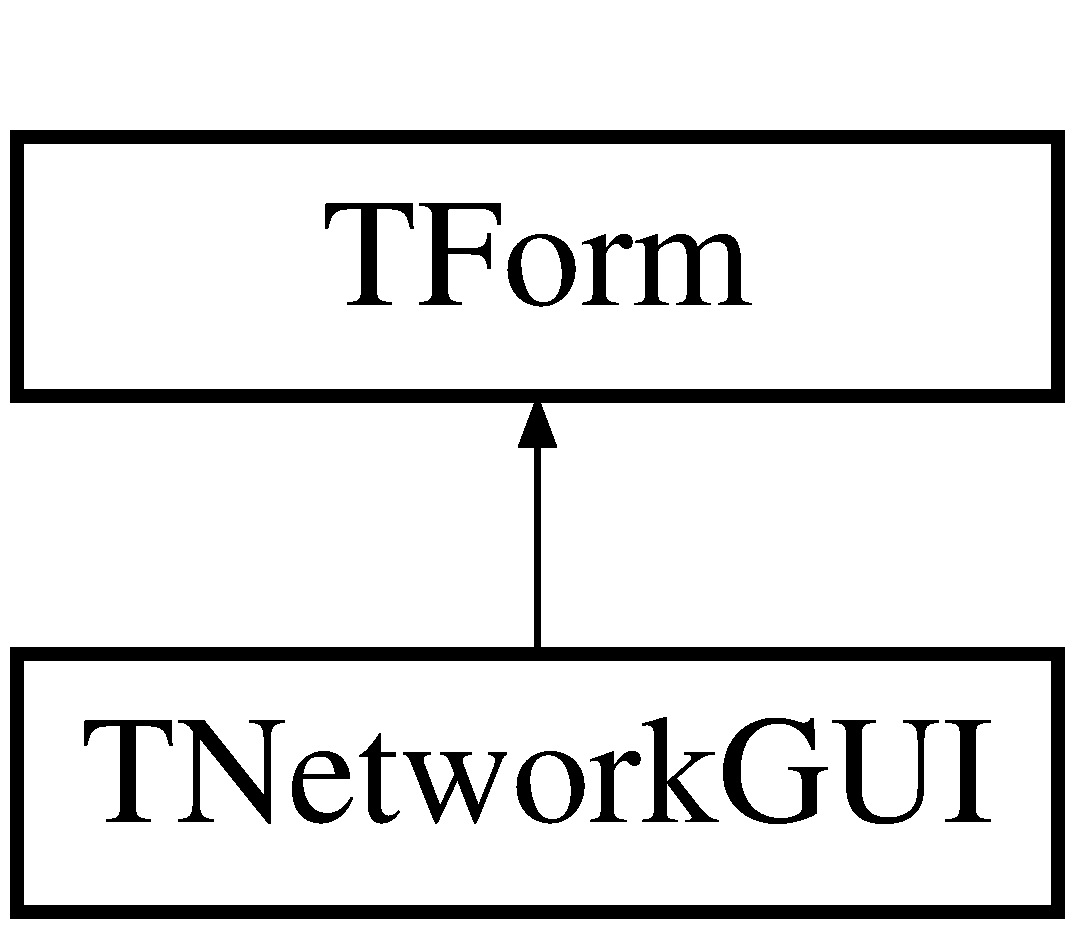
\includegraphics[height=2.000000cm]{class_t_network_g_u_i}
\end{center}
\end{figure}
\subsection*{Public Member Functions}
\begin{DoxyCompactItemize}
\item 
\hypertarget{class_t_network_g_u_i_a69805bd1ca490f7cfdb93ad4d02396a3}{void \+\_\+\+\_\+fastcall {\bfseries pmnu\+Network\+Popup} (T\+Object $\ast$Sender)}\label{class_t_network_g_u_i_a69805bd1ca490f7cfdb93ad4d02396a3}

\item 
\hypertarget{class_t_network_g_u_i_a91572bded8ffc3dec2a80b139dee0d43}{void \+\_\+\+\_\+fastcall {\bfseries Network\+Tree\+View\+Mouse\+Up} (T\+Object $\ast$Sender, T\+Mouse\+Button Button, T\+Shift\+State Shift, int X, int Y)}\label{class_t_network_g_u_i_a91572bded8ffc3dec2a80b139dee0d43}

\item 
\hypertarget{class_t_network_g_u_i_af4698aec82e6da7ca1344f2556369183}{void \+\_\+\+\_\+fastcall {\bfseries Remove\+Item1\+Click} (T\+Object $\ast$Sender)}\label{class_t_network_g_u_i_af4698aec82e6da7ca1344f2556369183}

\item 
\hypertarget{class_t_network_g_u_i_ae891d8bff24c1fb29233b2996888e5cf}{void \+\_\+\+\_\+fastcall {\bfseries Create\+Item1\+Click} (T\+Object $\ast$Sender)}\label{class_t_network_g_u_i_ae891d8bff24c1fb29233b2996888e5cf}

\item 
\hypertarget{class_t_network_g_u_i_a38a0e176bdb4e3b7ed9a41a92aadbcd7}{void \+\_\+\+\_\+fastcall {\bfseries Network\+Tree\+View\+Changing} (T\+Object $\ast$Sender, T\+Tree\+Node $\ast$Node, bool \&Allow\+Change)}\label{class_t_network_g_u_i_a38a0e176bdb4e3b7ed9a41a92aadbcd7}

\item 
\hypertarget{class_t_network_g_u_i_a74f52871b9d9eb774293cec2c07b63cb}{void \+\_\+\+\_\+fastcall {\bfseries Network\+Tree\+View\+Change} (T\+Object $\ast$Sender, T\+Tree\+Node $\ast$Node)}\label{class_t_network_g_u_i_a74f52871b9d9eb774293cec2c07b63cb}

\item 
\hypertarget{class_t_network_g_u_i_a1ddf3f343514af4a052d9b7185d0f83b}{void \+\_\+\+\_\+fastcall {\bfseries Action\+Create\+Cell\+Execute} (T\+Object $\ast$Sender)}\label{class_t_network_g_u_i_a1ddf3f343514af4a052d9b7185d0f83b}

\item 
\hypertarget{class_t_network_g_u_i_a7e81f9895cc22a62c9c8fe7afc84683c}{void \+\_\+\+\_\+fastcall {\bfseries Action\+Create\+Cell\+Update} (T\+Object $\ast$Sender)}\label{class_t_network_g_u_i_a7e81f9895cc22a62c9c8fe7afc84683c}

\item 
\hypertarget{class_t_network_g_u_i_a21750113c91893e4bc96e3c5fc9b5341}{void \+\_\+\+\_\+fastcall {\bfseries Action\+Create\+Synapse\+Execute} (T\+Object $\ast$Sender)}\label{class_t_network_g_u_i_a21750113c91893e4bc96e3c5fc9b5341}

\item 
\hypertarget{class_t_network_g_u_i_a455a4dbfb87092aa9f31f1b8d94cc915}{void \+\_\+\+\_\+fastcall {\bfseries Action\+Create\+Synapse\+Update} (T\+Object $\ast$Sender)}\label{class_t_network_g_u_i_a455a4dbfb87092aa9f31f1b8d94cc915}

\item 
\hypertarget{class_t_network_g_u_i_aa84f2d4ff3061491dd0e39e7d8961353}{void \+\_\+\+\_\+fastcall {\bfseries Action\+Create\+Electrode\+Execute} (T\+Object $\ast$Sender)}\label{class_t_network_g_u_i_aa84f2d4ff3061491dd0e39e7d8961353}

\item 
\hypertarget{class_t_network_g_u_i_aa6f3a85b99b456f7cead656aeea33057}{void \+\_\+\+\_\+fastcall {\bfseries Action\+Create\+Electrode\+Update} (T\+Object $\ast$Sender)}\label{class_t_network_g_u_i_aa6f3a85b99b456f7cead656aeea33057}

\item 
\hypertarget{class_t_network_g_u_i_ab5aa6e82815692e79755aa64be679aa3}{void \+\_\+\+\_\+fastcall {\bfseries File\+Open1\+Accept} (T\+Object $\ast$Sender)}\label{class_t_network_g_u_i_ab5aa6e82815692e79755aa64be679aa3}

\item 
\hypertarget{class_t_network_g_u_i_a309bb3756d0b0d57fd49c517f9687b96}{void \+\_\+\+\_\+fastcall {\bfseries File\+Save\+As1\+Accept} (T\+Object $\ast$Sender)}\label{class_t_network_g_u_i_a309bb3756d0b0d57fd49c517f9687b96}

\item 
\hypertarget{class_t_network_g_u_i_a9586d5cfe110f4f5f26d1ed088349ab0}{void \+\_\+\+\_\+fastcall {\bfseries Action\+Current\+Edit\+Execute} (T\+Object $\ast$Sender)}\label{class_t_network_g_u_i_a9586d5cfe110f4f5f26d1ed088349ab0}

\item 
\hypertarget{class_t_network_g_u_i_a02fc50defaacd0eafacbfa3265c59cde}{void \+\_\+\+\_\+fastcall {\bfseries Action\+Current\+Edit\+Update} (T\+Object $\ast$Sender)}\label{class_t_network_g_u_i_a02fc50defaacd0eafacbfa3265c59cde}

\item 
\hypertarget{class_t_network_g_u_i_a12517ab21c4d899be50f0c07f2032272}{void \+\_\+\+\_\+fastcall {\bfseries Action\+Run\+Execute} (T\+Object $\ast$Sender)}\label{class_t_network_g_u_i_a12517ab21c4d899be50f0c07f2032272}

\item 
\hypertarget{class_t_network_g_u_i_a660b34dd04a94b970a54bc9964ce3de8}{void \+\_\+\+\_\+fastcall {\bfseries Action\+Clear\+Network\+Execute} (T\+Object $\ast$Sender)}\label{class_t_network_g_u_i_a660b34dd04a94b970a54bc9964ce3de8}

\item 
\hypertarget{class_t_network_g_u_i_a7fe607193edb8ea0998adea49e314105}{void \+\_\+\+\_\+fastcall {\bfseries Action\+Remove\+Item\+Execute} (T\+Object $\ast$Sender)}\label{class_t_network_g_u_i_a7fe607193edb8ea0998adea49e314105}

\item 
\hypertarget{class_t_network_g_u_i_a63ebdd566386839f24347e18fa1decff}{void \+\_\+\+\_\+fastcall {\bfseries Network\+Tree\+View\+Edited} (T\+Object $\ast$Sender, T\+Tree\+Node $\ast$Node, Unicode\+String \&S)}\label{class_t_network_g_u_i_a63ebdd566386839f24347e18fa1decff}

\item 
\hypertarget{class_t_network_g_u_i_ad331603fe44bc47f68dac7df6cb56d3b}{void \+\_\+\+\_\+fastcall {\bfseries Network\+Tree\+View\+Editing} (T\+Object $\ast$Sender, T\+Tree\+Node $\ast$Node, bool \&Allow\+Edit)}\label{class_t_network_g_u_i_ad331603fe44bc47f68dac7df6cb56d3b}

\item 
\hypertarget{class_t_network_g_u_i_a76040e51bed8abf863018d30b6b9efb5}{void \+\_\+\+\_\+fastcall {\bfseries Network\+Tree\+View\+Dbl\+Click} (T\+Object $\ast$Sender)}\label{class_t_network_g_u_i_a76040e51bed8abf863018d30b6b9efb5}

\item 
\hypertarget{class_t_network_g_u_i_ae1598e335b16b4e708be702df0c239a3}{void \+\_\+\+\_\+fastcall {\bfseries Network\+Tree\+View\+Cancel\+Edit} (T\+Object $\ast$Sender, T\+Tree\+Node $\ast$Node)}\label{class_t_network_g_u_i_ae1598e335b16b4e708be702df0c239a3}

\item 
\hypertarget{class_t_network_g_u_i_a68da4c44df9e4f610d2cee97932d7f32}{void \+\_\+\+\_\+fastcall {\bfseries Network\+Tab\+Control\+Change} (T\+Object $\ast$Sender)}\label{class_t_network_g_u_i_a68da4c44df9e4f610d2cee97932d7f32}

\item 
\hypertarget{class_t_network_g_u_i_ad1f7b679669b5596faa4f54839d791c9}{void \+\_\+\+\_\+fastcall {\bfseries Network\+Tree\+View\+Mouse\+Move} (T\+Object $\ast$Sender, T\+Shift\+State Shift, int X, int Y)}\label{class_t_network_g_u_i_ad1f7b679669b5596faa4f54839d791c9}

\item 
\hypertarget{class_t_network_g_u_i_a64bc89cbffd96bd666494d36f8acf5b3}{void \+\_\+\+\_\+fastcall {\bfseries Copy\+Currents\+Action\+Execute} (T\+Object $\ast$Sender)}\label{class_t_network_g_u_i_a64bc89cbffd96bd666494d36f8acf5b3}

\item 
\hypertarget{class_t_network_g_u_i_a77217e3afbff8671e5669ad398329c30}{void \+\_\+\+\_\+fastcall {\bfseries File\+Open1\+Before\+Execute} (T\+Object $\ast$Sender)}\label{class_t_network_g_u_i_a77217e3afbff8671e5669ad398329c30}

\item 
\hypertarget{class_t_network_g_u_i_ade63c4e3eb3bdfdd0ed19ea62d889d62}{void \+\_\+\+\_\+fastcall {\bfseries File\+Save\+As1\+Before\+Execute} (T\+Object $\ast$Sender)}\label{class_t_network_g_u_i_ade63c4e3eb3bdfdd0ed19ea62d889d62}

\item 
\hypertarget{class_t_network_g_u_i_acbd47117ccdcf4c7ae80a71f28edc014}{void \+\_\+\+\_\+fastcall {\bfseries Collapse\+All1\+Click} (T\+Object $\ast$Sender)}\label{class_t_network_g_u_i_acbd47117ccdcf4c7ae80a71f28edc014}

\item 
\hypertarget{class_t_network_g_u_i_ad6c6cea6386a3fad7d82b565a155cb62}{bool \+\_\+\+\_\+fastcall {\bfseries Create\+Cell} (int X, int Y)}\label{class_t_network_g_u_i_ad6c6cea6386a3fad7d82b565a155cb62}

\item 
\hypertarget{class_t_network_g_u_i_abdbeac682dd72398d5595526288beb90}{bool \+\_\+\+\_\+fastcall {\bfseries Create\+Synapse} (const std\+::wstring \&First\+Cell\+Name, const std\+::wstring \&Second\+Cell\+Name, int X, int Y)}\label{class_t_network_g_u_i_abdbeac682dd72398d5595526288beb90}

\item 
\hypertarget{class_t_network_g_u_i_ad7e300956e9f1475d9ca86185fd5b31c}{bool \+\_\+\+\_\+fastcall {\bfseries Create\+Electrode} (const std\+::wstring \&cellname, int X, int Y)}\label{class_t_network_g_u_i_ad7e300956e9f1475d9ca86185fd5b31c}

\item 
\hypertarget{class_t_network_g_u_i_a80f01942447154bb5a241b3d295bfe82}{\+\_\+\+\_\+fastcall {\bfseries T\+Network\+G\+U\+I} (T\+Component $\ast$Owner)}\label{class_t_network_g_u_i_a80f01942447154bb5a241b3d295bfe82}

\end{DoxyCompactItemize}
\subsection*{Public Attributes}
\begin{DoxyCompactItemize}
\item 
\hypertarget{class_t_network_g_u_i_abdc95a48f6b4cc13fa72d39d85d62899}{T\+Action\+Manager $\ast$ {\bfseries Action\+Manager1}}\label{class_t_network_g_u_i_abdc95a48f6b4cc13fa72d39d85d62899}

\item 
\hypertarget{class_t_network_g_u_i_aebc2596d63e6d20e48deeccdd055e465}{T\+Action\+Main\+Menu\+Bar $\ast$ {\bfseries Action\+Main\+Menu\+Bar1}}\label{class_t_network_g_u_i_aebc2596d63e6d20e48deeccdd055e465}

\item 
\hypertarget{class_t_network_g_u_i_a0e91f1e4d5d0b1fb1459390c29159658}{T\+Action\+Tool\+Bar $\ast$ {\bfseries Action\+Tool\+Bar1}}\label{class_t_network_g_u_i_a0e91f1e4d5d0b1fb1459390c29159658}

\item 
\hypertarget{class_t_network_g_u_i_a4077aff685393ce61aee72dc353b3fe7}{T\+Image\+List $\ast$ {\bfseries Image\+List1}}\label{class_t_network_g_u_i_a4077aff685393ce61aee72dc353b3fe7}

\item 
\hypertarget{class_t_network_g_u_i_a608a03d14df65502a599b887a1626906}{T\+Image\+List $\ast$ {\bfseries Image\+List2}}\label{class_t_network_g_u_i_a608a03d14df65502a599b887a1626906}

\item 
\hypertarget{class_t_network_g_u_i_aca116a4f60cc788ea706b01ee517416b}{T\+Panel $\ast$ {\bfseries Panel1}}\label{class_t_network_g_u_i_aca116a4f60cc788ea706b01ee517416b}

\item 
\hypertarget{class_t_network_g_u_i_a142450d7f621a15d9c73b5e45c4e7915}{T\+Panel $\ast$ {\bfseries Panel2}}\label{class_t_network_g_u_i_a142450d7f621a15d9c73b5e45c4e7915}

\item 
\hypertarget{class_t_network_g_u_i_a8ff68f2827c87fd0c77c77cea7b7d135}{T\+Panel $\ast$ {\bfseries Panel3}}\label{class_t_network_g_u_i_a8ff68f2827c87fd0c77c77cea7b7d135}

\item 
\hypertarget{class_t_network_g_u_i_a7a98e38a3d80a4c558d75c1fc27246bd}{T\+Popup\+Menu $\ast$ {\bfseries pmnu\+Network}}\label{class_t_network_g_u_i_a7a98e38a3d80a4c558d75c1fc27246bd}

\item 
\hypertarget{class_t_network_g_u_i_aef13ef2788870ed25de8fa8f302cb3fe}{T\+Menu\+Item $\ast$ {\bfseries Remove\+Item1}}\label{class_t_network_g_u_i_aef13ef2788870ed25de8fa8f302cb3fe}

\item 
\hypertarget{class_t_network_g_u_i_a05b08e1472ec6c2a3eb697684331bfcc}{T\+Splitter $\ast$ {\bfseries Splitter1}}\label{class_t_network_g_u_i_a05b08e1472ec6c2a3eb697684331bfcc}

\item 
\hypertarget{class_t_network_g_u_i_ae9941e8e08025b9dbf0e6c2036cf309c}{T\+Action $\ast$ {\bfseries Action\+Create\+Cell}}\label{class_t_network_g_u_i_ae9941e8e08025b9dbf0e6c2036cf309c}

\item 
\hypertarget{class_t_network_g_u_i_a5948045e066b60273ec9b45f3c1238a9}{T\+Action $\ast$ {\bfseries Action\+Create\+Synapse}}\label{class_t_network_g_u_i_a5948045e066b60273ec9b45f3c1238a9}

\item 
\hypertarget{class_t_network_g_u_i_aab2ec986f74e1ec192e96bd64c85bf5a}{T\+Action $\ast$ {\bfseries Action\+Create\+Electrode}}\label{class_t_network_g_u_i_aab2ec986f74e1ec192e96bd64c85bf5a}

\item 
\hypertarget{class_t_network_g_u_i_aa138efcd0f908c53848b9cf696c63044}{T\+Scroll\+Box $\ast$ {\bfseries Network\+Component\+Edit\+Scroll\+Box}}\label{class_t_network_g_u_i_aa138efcd0f908c53848b9cf696c63044}

\item 
\hypertarget{class_t_network_g_u_i_a52f28057fa7a38ae63169b38a35ea2e7}{T\+Generic\+Utilities $\ast$ {\bfseries Generic\+Utilities1}}\label{class_t_network_g_u_i_a52f28057fa7a38ae63169b38a35ea2e7}

\item 
\hypertarget{class_t_network_g_u_i_aa77be94fb66cff42fd26b52709aaf05e}{T\+Action\+Tool\+Bar $\ast$ {\bfseries Action\+Tool\+Bar2}}\label{class_t_network_g_u_i_aa77be94fb66cff42fd26b52709aaf05e}

\item 
\hypertarget{class_t_network_g_u_i_af481478dd4a11e6ad88e8a93db33f4d1}{T\+File\+Open $\ast$ {\bfseries File\+Open1}}\label{class_t_network_g_u_i_af481478dd4a11e6ad88e8a93db33f4d1}

\item 
\hypertarget{class_t_network_g_u_i_a13837c38fc985da34c510f6359784b6b}{T\+File\+Save\+As $\ast$ {\bfseries File\+Save\+As1}}\label{class_t_network_g_u_i_a13837c38fc985da34c510f6359784b6b}

\item 
\hypertarget{class_t_network_g_u_i_af609532f22c0ebbda05f71f6ac878468}{T\+Action $\ast$ {\bfseries Action\+Current\+Edit}}\label{class_t_network_g_u_i_af609532f22c0ebbda05f71f6ac878468}

\item 
\hypertarget{class_t_network_g_u_i_a6bd661e661fb7021b69191d79ec54c86}{T\+Action $\ast$ {\bfseries Action\+Run}}\label{class_t_network_g_u_i_a6bd661e661fb7021b69191d79ec54c86}

\item 
\hypertarget{class_t_network_g_u_i_a04f47dbc35e7dadbd6c88253dcad3761}{T\+Action $\ast$ {\bfseries Action\+Clear\+Network}}\label{class_t_network_g_u_i_a04f47dbc35e7dadbd6c88253dcad3761}

\item 
\hypertarget{class_t_network_g_u_i_a62363debe1b2b47e137d4658e8d89110}{T\+Panel $\ast$ {\bfseries Panel4}}\label{class_t_network_g_u_i_a62363debe1b2b47e137d4658e8d89110}

\item 
\hypertarget{class_t_network_g_u_i_ad6378f68c33c5506887a61f529e5e7a1}{T\+Tree\+View $\ast$ {\bfseries Network\+Tree\+View}}\label{class_t_network_g_u_i_ad6378f68c33c5506887a61f529e5e7a1}

\item 
\hypertarget{class_t_network_g_u_i_a21862087fff3dfd5d5128e0172b40f81}{T\+Panel $\ast$ {\bfseries Panel5}}\label{class_t_network_g_u_i_a21862087fff3dfd5d5128e0172b40f81}

\item 
\hypertarget{class_t_network_g_u_i_acb046470596d359be16b66847a969ff5}{T\+Action\+Tool\+Bar $\ast$ {\bfseries Action\+Tool\+Bar3}}\label{class_t_network_g_u_i_acb046470596d359be16b66847a969ff5}

\item 
\hypertarget{class_t_network_g_u_i_ad4bea929fb181e3b80e9f5ba21a90f23}{T\+Action $\ast$ {\bfseries Action\+Remove\+Item}}\label{class_t_network_g_u_i_ad4bea929fb181e3b80e9f5ba21a90f23}

\item 
\hypertarget{class_t_network_g_u_i_aef2d4166191cf6f16fe43c637a79038b}{T\+Panel $\ast$ {\bfseries Panel10}}\label{class_t_network_g_u_i_aef2d4166191cf6f16fe43c637a79038b}

\item 
\hypertarget{class_t_network_g_u_i_a22cba9f3ddec6bbbff949ea22a0191aa}{T\+Splitter $\ast$ {\bfseries Splitter2}}\label{class_t_network_g_u_i_a22cba9f3ddec6bbbff949ea22a0191aa}

\item 
\hypertarget{class_t_network_g_u_i_a5fdd5dd306aa0ac455aca6bb792d9b72}{T\+Panel $\ast$ {\bfseries Network\+Panel}}\label{class_t_network_g_u_i_a5fdd5dd306aa0ac455aca6bb792d9b72}

\item 
\hypertarget{class_t_network_g_u_i_a4f3b92e132a0735d61f5e746c1fcf00b}{T\+Tab\+Control $\ast$ {\bfseries Network\+Tab\+Control}}\label{class_t_network_g_u_i_a4f3b92e132a0735d61f5e746c1fcf00b}

\item 
\hypertarget{class_t_network_g_u_i_a269417f3eb8d10576134809b9c312bb1}{T\+Action $\ast$ {\bfseries Action\+Version\+Info}}\label{class_t_network_g_u_i_a269417f3eb8d10576134809b9c312bb1}

\item 
\hypertarget{class_t_network_g_u_i_a9782b2344ac6181536a0c66984d70594}{T\+Action $\ast$ {\bfseries Copy\+Currents\+Action}}\label{class_t_network_g_u_i_a9782b2344ac6181536a0c66984d70594}

\item 
\hypertarget{class_t_network_g_u_i_a90aaebf113d9babf37b2851262f202aa}{T\+Menu\+Item $\ast$ {\bfseries Collapse\+All1}}\label{class_t_network_g_u_i_a90aaebf113d9babf37b2851262f202aa}

\item 
\hypertarget{class_t_network_g_u_i_a43e4e90e4968db4857a905f648bcec24}{int {\bfseries Model\+Mouse\+Mode}}\label{class_t_network_g_u_i_a43e4e90e4968db4857a905f648bcec24}

\end{DoxyCompactItemize}


\subsection{Detailed Description}
Graphical interface for creating, editing, and running a network. 

Master network builder and editor that contains 3 regions\+:
\begin{DoxyItemize}
\item An area with forms for designing connections (\hyperlink{class_t_g_u_i___circle_perimeter_form}{T\+G\+U\+I\+\_\+\+Circle\+Perimeter\+Form} and \hyperlink{class_t_g_u_i___square_lattice_form}{T\+G\+U\+I\+\_\+\+Square\+Lattice\+Form})
\item A \char`\"{}tree\char`\"{} organization of the network that is used for selecting network elements, and
\item An area to display the G\+U\+I edit forms for the selected network component.
\end{DoxyItemize}

\begin{DoxyAuthor}{Author}
E. Brady Trexler $<$ebtrexler (at) gothamsci.\+com$>$, 2011 -\/ 2013 
\end{DoxyAuthor}


The documentation for this class was generated from the following files\+:\begin{DoxyCompactItemize}
\item 
G\+U\+I\+\_\+\+Network\+Form.\+h\item 
G\+U\+I\+\_\+\+Network\+Form.\+cpp\end{DoxyCompactItemize}

\hypertarget{class_t_periodicity_form}{\section{T\+Periodicity\+Form Class Reference}
\label{class_t_periodicity_form}\index{T\+Periodicity\+Form@{T\+Periodicity\+Form}}
}


G\+U\+I Editor for periodicity settings of various currents.  




{\ttfamily \#include $<$G\+U\+I\+\_\+\+Periodicity\+Editor.\+h$>$}

Inheritance diagram for T\+Periodicity\+Form\+:\begin{figure}[H]
\begin{center}
\leavevmode
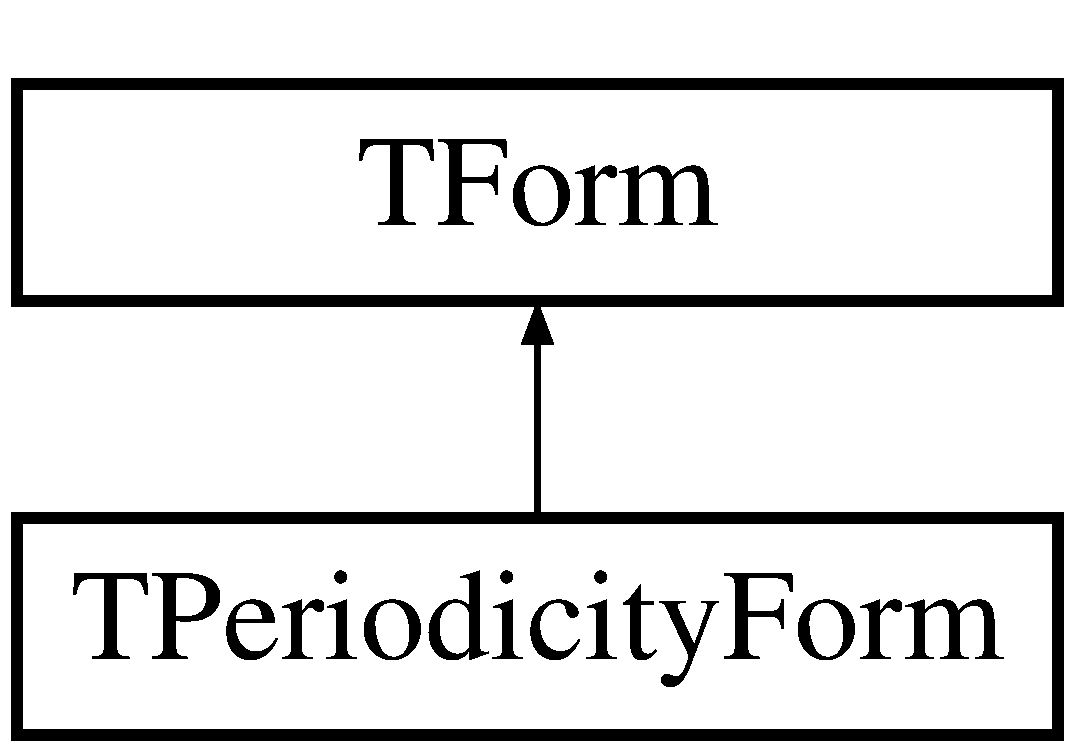
\includegraphics[height=2.000000cm]{class_t_periodicity_form}
\end{center}
\end{figure}
\subsection*{Public Member Functions}
\begin{DoxyCompactItemize}
\item 
\hypertarget{class_t_periodicity_form_a45622b2dd251e376d852d18a61d955e4}{\+\_\+\+\_\+fastcall {\bfseries T\+Periodicity\+Form} (T\+Component $\ast$Owner)}\label{class_t_periodicity_form_a45622b2dd251e376d852d18a61d955e4}

\end{DoxyCompactItemize}
\subsection*{Public Attributes}
\begin{DoxyCompactItemize}
\item 
\hypertarget{class_t_periodicity_form_abe96fee6cde704ea5663c2c1a43e30f4}{T\+Value\+List\+Editor $\ast$ {\bfseries Value\+List\+Editor1}}\label{class_t_periodicity_form_abe96fee6cde704ea5663c2c1a43e30f4}

\item 
\hypertarget{class_t_periodicity_form_af7c0dbe49e6b28026a16e32230cafa2d}{T\+Button $\ast$ {\bfseries Ok\+Button}}\label{class_t_periodicity_form_af7c0dbe49e6b28026a16e32230cafa2d}

\item 
\hypertarget{class_t_periodicity_form_a41b6b7cac8f7b7aa5710674a97e16d7b}{T\+Button $\ast$ {\bfseries Cancel\+Button}}\label{class_t_periodicity_form_a41b6b7cac8f7b7aa5710674a97e16d7b}

\item 
\hypertarget{class_t_periodicity_form_a29b23177f4216ee8a96b5dc1c4231e8e}{T\+Label $\ast$ {\bfseries Label1}}\label{class_t_periodicity_form_a29b23177f4216ee8a96b5dc1c4231e8e}

\item 
\hypertarget{class_t_periodicity_form_accef9585dcb1f56ff2ff902987c92f00}{T\+Combo\+Box $\ast$ {\bfseries Waveform\+Type\+Combo\+Box}}\label{class_t_periodicity_form_accef9585dcb1f56ff2ff902987c92f00}

\item 
\hypertarget{class_t_periodicity_form_a3eabb795215c595abb801ddcc07946e7}{T\+Label $\ast$ {\bfseries Label2}}\label{class_t_periodicity_form_a3eabb795215c595abb801ddcc07946e7}

\end{DoxyCompactItemize}


\subsection{Detailed Description}
G\+U\+I Editor for periodicity settings of various currents. 

\begin{DoxyAuthor}{Author}
E. Brady Trexler $<$ebtrexler (at) gothamsci.\+com$>$, 2011 -\/ 2013 
\end{DoxyAuthor}


The documentation for this class was generated from the following files\+:\begin{DoxyCompactItemize}
\item 
G\+U\+I\+\_\+\+Periodicity\+Editor.\+h\item 
G\+U\+I\+\_\+\+Periodicity\+Editor.\+cpp\end{DoxyCompactItemize}

\hypertarget{class_t_playback_cell}{\section{T\+Playback\+Cell Class Reference}
\label{class_t_playback_cell}\index{T\+Playback\+Cell@{T\+Playback\+Cell}}
}


Derived class that implements model cell that plays back pre-\/recorded Vm.  


Inheritance diagram for T\+Playback\+Cell\+:\begin{figure}[H]
\begin{center}
\leavevmode
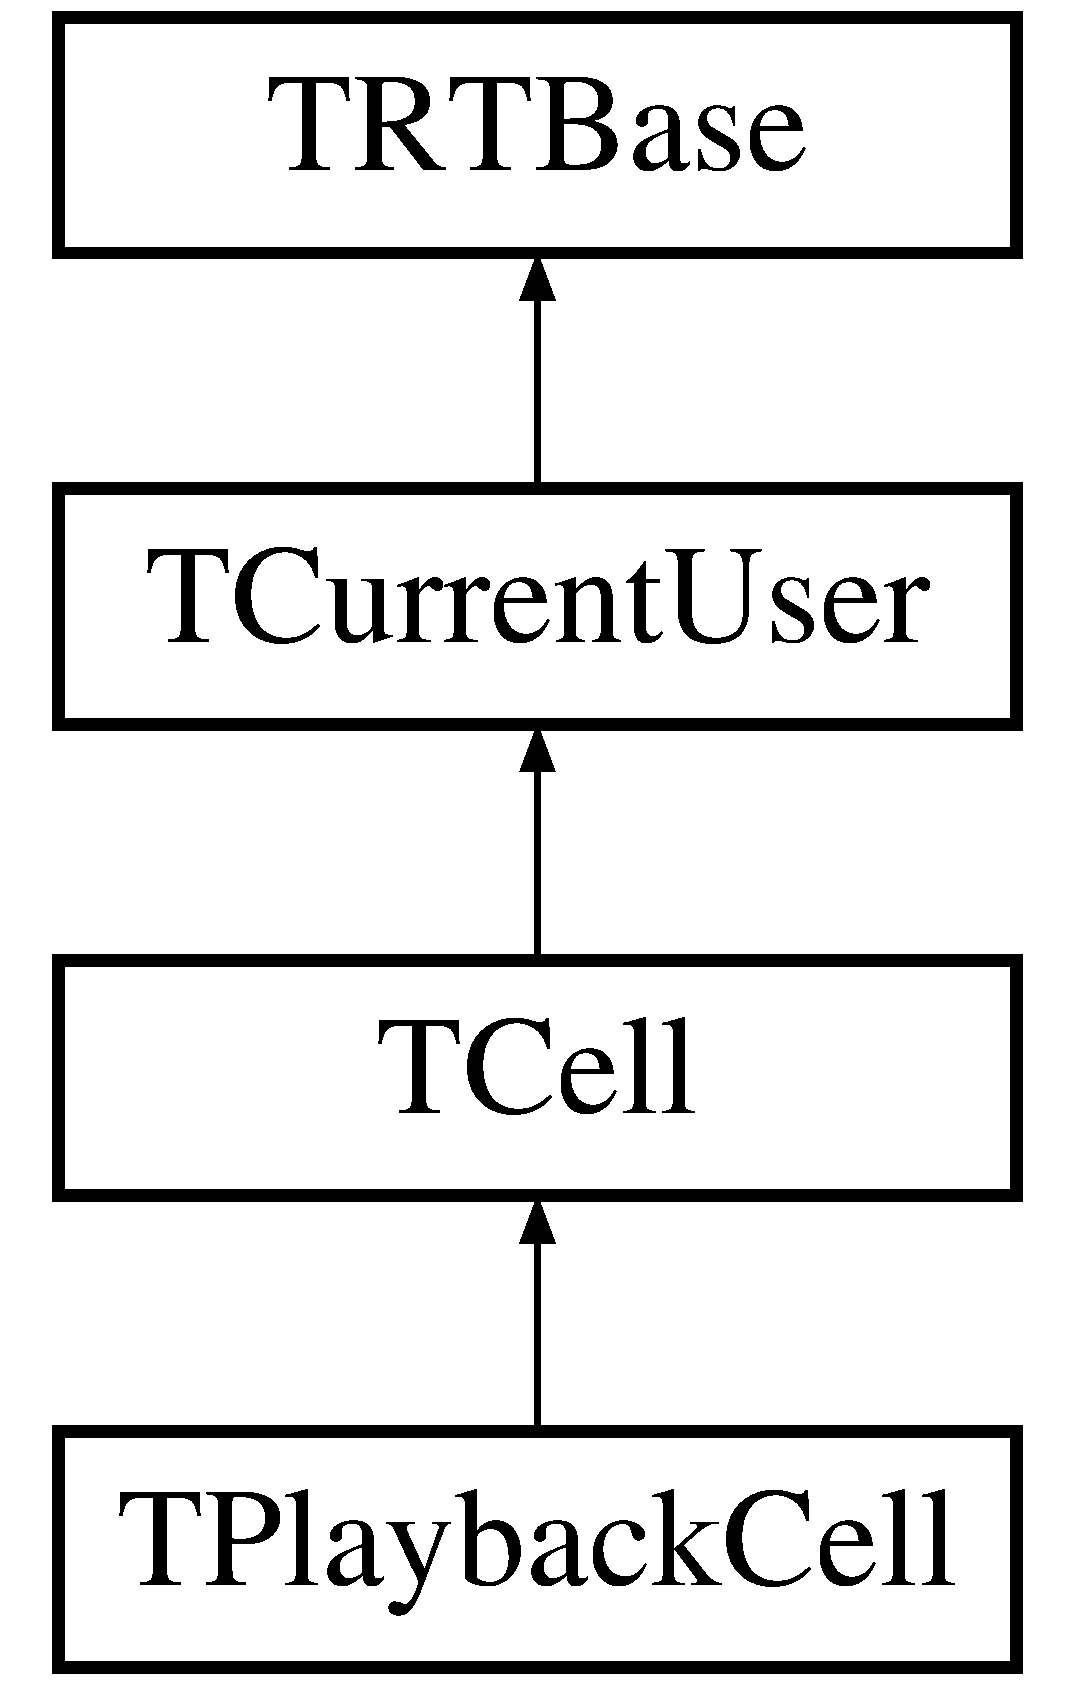
\includegraphics[height=4.000000cm]{class_t_playback_cell}
\end{center}
\end{figure}
\subsection*{Public Member Functions}
\begin{DoxyCompactItemize}
\item 
\hypertarget{class_t_playback_cell_ac6cc9092b073fa782d455da1bbb14916}{\+\_\+\+\_\+fastcall {\bfseries T\+Playback\+Cell} (const std\+::wstring \&name)}\label{class_t_playback_cell_ac6cc9092b073fa782d455da1bbb14916}

\item 
\hypertarget{class_t_playback_cell_ac48549662a7ca95cbd35b2f9b3abe250}{virtual \hyperlink{class_t_playback_waveform}{T\+Playback\+Waveform} \\*
$\ast$const \+\_\+\+\_\+fastcall {\bfseries Get\+Playback\+Waveform} ()}\label{class_t_playback_cell_ac48549662a7ca95cbd35b2f9b3abe250}

\item 
virtual void $\ast$const \+\_\+\+\_\+fastcall \hyperlink{class_t_playback_cell_a5cd1500e6e80753779d7dee74f4b84d2}{Get\+Edit\+Form} ()
\item 
\hypertarget{class_t_playback_cell_a755c17c4499e465d02952e59689b5196}{virtual void \+\_\+\+\_\+fastcall \hyperlink{class_t_playback_cell_a755c17c4499e465d02952e59689b5196}{Populate\+Edit\+Form} ()}\label{class_t_playback_cell_a755c17c4499e465d02952e59689b5196}

\begin{DoxyCompactList}\small\item\em Interface for derived classes, called by G\+U\+I to update V\+C\+L form components. \end{DoxyCompactList}\item 
\hypertarget{class_t_playback_cell_abaae8a711796f5a8aa3498aefbd30c8c}{virtual bool \+\_\+\+\_\+fastcall \hyperlink{class_t_playback_cell_abaae8a711796f5a8aa3498aefbd30c8c}{Validate\+Edit\+Form} ()}\label{class_t_playback_cell_abaae8a711796f5a8aa3498aefbd30c8c}

\begin{DoxyCompactList}\small\item\em Interface for derived classes, called by G\+U\+I to read V\+C\+L form values. \end{DoxyCompactList}\item 
\hypertarget{class_t_playback_cell_a0794ca1e720afeb431a91c850b976003}{virtual double \+\_\+\+\_\+fastcall \hyperlink{class_t_playback_cell_a0794ca1e720afeb431a91c850b976003}{Set\+Vm} (double \hyperlink{class_t_cell_afd81f2fd923ffbfa5ea7eda2c50693d1}{Vm})}\label{class_t_playback_cell_a0794ca1e720afeb431a91c850b976003}

\begin{DoxyCompactList}\small\item\em Sets the membrane voltage. \end{DoxyCompactList}\item 
\hypertarget{class_t_playback_cell_a32c5642349a72c44ff317fd172b9a121}{virtual double \+\_\+\+\_\+fastcall \hyperlink{class_t_playback_cell_a32c5642349a72c44ff317fd172b9a121}{Calc\+Vm} (double step)}\label{class_t_playback_cell_a32c5642349a72c44ff317fd172b9a121}

\begin{DoxyCompactList}\small\item\em Calculates the voltage given the step in ms. \end{DoxyCompactList}\item 
\hypertarget{class_t_playback_cell_a69ee14c129bcaf44ff40c14c2c66569b}{bool \+\_\+\+\_\+fastcall \hyperlink{class_t_playback_cell_a69ee14c129bcaf44ff40c14c2c66569b}{Is\+Voltage\+Dependent} ()}\label{class_t_playback_cell_a69ee14c129bcaf44ff40c14c2c66569b}

\begin{DoxyCompactList}\small\item\em Returns false, because this cell exists only in software. \end{DoxyCompactList}\item 
\hypertarget{class_t_playback_cell_a7dd6c3c0c873d74e767ce4881954f20b}{bool \+\_\+\+\_\+fastcall \hyperlink{class_t_playback_cell_a7dd6c3c0c873d74e767ce4881954f20b}{Initialize} (bool Reset)}\label{class_t_playback_cell_a7dd6c3c0c873d74e767ce4881954f20b}

\begin{DoxyCompactList}\small\item\em pure virtual function for resetting before networking run \end{DoxyCompactList}\item 
const std\+::wstring \&\+\_\+\+\_\+fastcall \hyperlink{class_t_playback_cell_a8e35ecdb1be99d97349d8904b6064e5d}{Class\+Key} () const 
\begin{DoxyCompactList}\small\item\em Returns string used to register class with factory. \end{DoxyCompactList}\item 
\hypertarget{class_t_playback_cell_aa6230016ea05dc27519729aa7bc38c0f}{virtual const \hyperlink{class_t_current}{T\+Current} $\ast$\+\_\+\+\_\+fastcall \hyperlink{class_t_playback_cell_aa6230016ea05dc27519729aa7bc38c0f}{Add\+Current} (\hyperlink{class_t_current}{T\+Current} $\ast$const c, \hyperlink{class_t_cell}{T\+Cell} $\ast$cell=N\+U\+L\+L)}\label{class_t_playback_cell_aa6230016ea05dc27519729aa7bc38c0f}

\begin{DoxyCompactList}\small\item\em Overrides and disables adding a \hyperlink{class_t_current}{T\+Current} $\ast$ to the array of Currents. \end{DoxyCompactList}\item 
\hypertarget{class_t_playback_cell_a736a499f823cd99dc2fb0c30c9940d40}{virtual const \hyperlink{class_t_electrode}{T\+Electrode} \\*
$\ast$\+\_\+\+\_\+fastcall \hyperlink{class_t_playback_cell_a736a499f823cd99dc2fb0c30c9940d40}{Add\+Electrode} (\hyperlink{class_t_electrode}{T\+Electrode} $\ast$e)}\label{class_t_playback_cell_a736a499f823cd99dc2fb0c30c9940d40}

\begin{DoxyCompactList}\small\item\em Overrides and disables adding a \hyperlink{class_t_electrode}{T\+Electrode} $\ast$ to the array of Electrodes. \end{DoxyCompactList}\item 
\hypertarget{class_t_playback_cell_a6f8d8d938e012adc17c8cd44e936e1b6}{virtual const bool \+\_\+\+\_\+fastcall \hyperlink{class_t_playback_cell_a6f8d8d938e012adc17c8cd44e936e1b6}{Accepts\+Currents} () const }\label{class_t_playback_cell_a6f8d8d938e012adc17c8cd44e936e1b6}

\begin{DoxyCompactList}\small\item\em Informs caller whether can accept currents or not. \end{DoxyCompactList}\item 
\hypertarget{class_t_playback_cell_a16763fa74c03646eface33316a938756}{virtual double \+\_\+\+\_\+fastcall \hyperlink{class_t_playback_cell_a16763fa74c03646eface33316a938756}{Do\+Update} (double step)}\label{class_t_playback_cell_a16763fa74c03646eface33316a938756}

\begin{DoxyCompactList}\small\item\em Disables current calculations because there aren't any. \end{DoxyCompactList}\end{DoxyCompactItemize}
\subsection*{Friends}
\begin{DoxyCompactItemize}
\item 
\hypertarget{class_t_playback_cell_ac98d07dd8f7b70e16ccb9a01abf56b9c}{class \hyperlink{class_t_playback_cell_ac98d07dd8f7b70e16ccb9a01abf56b9c}{boost\+::serialization\+::access}}\label{class_t_playback_cell_ac98d07dd8f7b70e16ccb9a01abf56b9c}

\begin{DoxyCompactList}\small\item\em Required for serialization and saving networks to disk. \end{DoxyCompactList}\end{DoxyCompactItemize}
\subsection*{Additional Inherited Members}


\subsection{Detailed Description}
Derived class that implements model cell that plays back pre-\/recorded Vm. 

It can contain no currents. Appropriate methods are overridden.

\begin{DoxyAuthor}{Author}
E. Brady Trexler $<$ebtrexler (at) gothamsci.\+com$>$, 2011 -\/ 2013 
\end{DoxyAuthor}


\subsection{Member Function Documentation}
\hypertarget{class_t_playback_cell_a8e35ecdb1be99d97349d8904b6064e5d}{\index{T\+Playback\+Cell@{T\+Playback\+Cell}!Class\+Key@{Class\+Key}}
\index{Class\+Key@{Class\+Key}!T\+Playback\+Cell@{T\+Playback\+Cell}}
\subsubsection[{Class\+Key}]{\setlength{\rightskip}{0pt plus 5cm}const std\+::wstring\& \+\_\+\+\_\+fastcall T\+Playback\+Cell\+::\+Class\+Key (
\begin{DoxyParamCaption}
{}
\end{DoxyParamCaption}
) const\hspace{0.3cm}{\ttfamily [inline]}, {\ttfamily [virtual]}}}\label{class_t_playback_cell_a8e35ecdb1be99d97349d8904b6064e5d}


Returns string used to register class with factory. 

Users of class factories must also tell the class the key they used when registering the class. See factory.\+h 

Implements \hyperlink{class_t_r_t_base_a6083fd510cbcb00faa85e5934fc3c18e}{T\+R\+T\+Base}.

\hypertarget{class_t_playback_cell_a5cd1500e6e80753779d7dee74f4b84d2}{\index{T\+Playback\+Cell@{T\+Playback\+Cell}!Get\+Edit\+Form@{Get\+Edit\+Form}}
\index{Get\+Edit\+Form@{Get\+Edit\+Form}!T\+Playback\+Cell@{T\+Playback\+Cell}}
\subsubsection[{Get\+Edit\+Form}]{\setlength{\rightskip}{0pt plus 5cm}virtual void$\ast$ const \+\_\+\+\_\+fastcall T\+Playback\+Cell\+::\+Get\+Edit\+Form (
\begin{DoxyParamCaption}
{}
\end{DoxyParamCaption}
)\hspace{0.3cm}{\ttfamily [inline]}, {\ttfamily [virtual]}}}\label{class_t_playback_cell_a5cd1500e6e80753779d7dee74f4b84d2}
Interface for derived classes, returns pointer to G\+U\+I object for editing members. Callers must cast pointer to the correct object. 

Implements \hyperlink{class_t_r_t_base_ab83e520005e20ee71f98f3e85e1ee6d4}{T\+R\+T\+Base}.



The documentation for this class was generated from the following file\+:\begin{DoxyCompactItemize}
\item 
G\+U\+I\+\_\+\+R\+T\+\_\+\+Edit\+\_\+\+Playback\+Cell.\+cpp\end{DoxyCompactItemize}

\hypertarget{class_t_playback_cell_form}{\section{T\+Playback\+Cell\+Form Class Reference}
\label{class_t_playback_cell_form}\index{T\+Playback\+Cell\+Form@{T\+Playback\+Cell\+Form}}
}


G\+U\+I Editor for \hyperlink{class_t_playback_cell}{T\+Playback\+Cell}.  




{\ttfamily \#include $<$G\+U\+I\+\_\+\+R\+T\+\_\+\+Edit\+\_\+\+Playback\+Cell.\+h$>$}

Inheritance diagram for T\+Playback\+Cell\+Form\+:\begin{figure}[H]
\begin{center}
\leavevmode
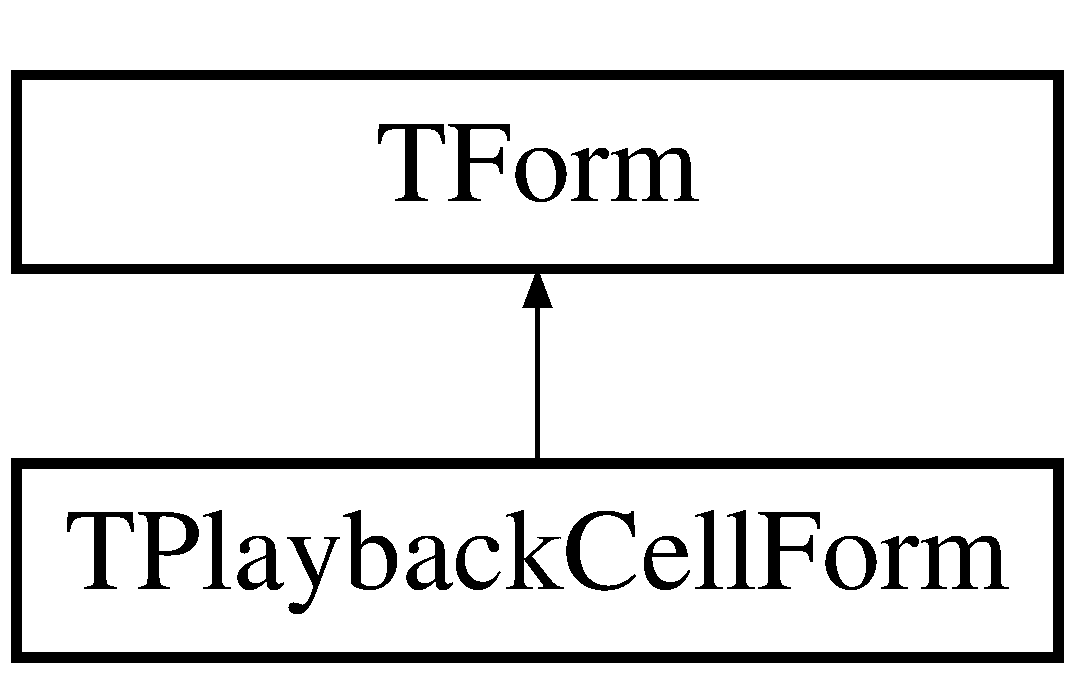
\includegraphics[height=2.000000cm]{class_t_playback_cell_form}
\end{center}
\end{figure}
\subsection*{Public Member Functions}
\begin{DoxyCompactItemize}
\item 
\hypertarget{class_t_playback_cell_form_a9ddd7c0eb2f14078fbe9227245162630}{void \+\_\+\+\_\+fastcall {\bfseries Browse\+Bit\+Btn\+Click} (T\+Object $\ast$Sender)}\label{class_t_playback_cell_form_a9ddd7c0eb2f14078fbe9227245162630}

\item 
\hypertarget{class_t_playback_cell_form_a31241fdb5b23e233cff3f60d7f9e2bd8}{void \+\_\+\+\_\+fastcall {\bfseries Channel\+Combo\+Box\+Change} (T\+Object $\ast$Sender)}\label{class_t_playback_cell_form_a31241fdb5b23e233cff3f60d7f9e2bd8}

\item 
\hypertarget{class_t_playback_cell_form_a5cbf97d59d4b022a81cbcb23515cdc8f}{void \+\_\+\+\_\+fastcall {\bfseries Convertm\+V\+Edit\+Key\+Press} (T\+Object $\ast$Sender, wchar\+\_\+t \&Key)}\label{class_t_playback_cell_form_a5cbf97d59d4b022a81cbcb23515cdc8f}

\item 
\hypertarget{class_t_playback_cell_form_a7c7022532ad563f28b1791804a2f189f}{\+\_\+\+\_\+fastcall {\bfseries T\+Playback\+Cell\+Form} (T\+Component $\ast$Owner)}\label{class_t_playback_cell_form_a7c7022532ad563f28b1791804a2f189f}

\end{DoxyCompactItemize}
\subsection*{Public Attributes}
\begin{DoxyCompactItemize}
\item 
\hypertarget{class_t_playback_cell_form_a2ff8cd78c08f73842ce568a7d0805417}{T\+Open\+Dialog $\ast$ {\bfseries Open\+Dialog1}}\label{class_t_playback_cell_form_a2ff8cd78c08f73842ce568a7d0805417}

\item 
\hypertarget{class_t_playback_cell_form_a3e9f5ab9b08b582daf8d67bf18d9e83d}{T\+Image\+List $\ast$ {\bfseries Image\+List1}}\label{class_t_playback_cell_form_a3e9f5ab9b08b582daf8d67bf18d9e83d}

\item 
\hypertarget{class_t_playback_cell_form_a128f9d7e30dbcc0acde13d1ebdc959da}{T\+P\+L\+O\+T\+Panel $\ast$ {\bfseries P\+L\+O\+T\+Panel1}}\label{class_t_playback_cell_form_a128f9d7e30dbcc0acde13d1ebdc959da}

\item 
\hypertarget{class_t_playback_cell_form_aa835b8dd7f9bb680efba342782c2cefb}{T\+Label $\ast$ {\bfseries Label1}}\label{class_t_playback_cell_form_aa835b8dd7f9bb680efba342782c2cefb}

\item 
\hypertarget{class_t_playback_cell_form_a17a38029a70c4075b1cdec3021052436}{T\+Label $\ast$ {\bfseries File\+Label}}\label{class_t_playback_cell_form_a17a38029a70c4075b1cdec3021052436}

\item 
\hypertarget{class_t_playback_cell_form_a6c6f1625ee45628851514948a7862999}{T\+Bit\+Btn $\ast$ {\bfseries Browse\+Bit\+Btn}}\label{class_t_playback_cell_form_a6c6f1625ee45628851514948a7862999}

\item 
\hypertarget{class_t_playback_cell_form_a1e276cafeb696b752c80dafbe581523d}{T\+Label $\ast$ {\bfseries Label2}}\label{class_t_playback_cell_form_a1e276cafeb696b752c80dafbe581523d}

\item 
\hypertarget{class_t_playback_cell_form_af7e76b364f7c2763f72ca9a92a4fac82}{T\+Combo\+Box $\ast$ {\bfseries Channel\+Combo\+Box}}\label{class_t_playback_cell_form_af7e76b364f7c2763f72ca9a92a4fac82}

\item 
\hypertarget{class_t_playback_cell_form_a5ca949f0d215dc6d3ef219d96f733686}{T\+Label $\ast$ {\bfseries Label3}}\label{class_t_playback_cell_form_a5ca949f0d215dc6d3ef219d96f733686}

\item 
\hypertarget{class_t_playback_cell_form_a051e3e5ba88389b241acecdc60789e2a}{T\+Edit $\ast$ {\bfseries Convertm\+V\+Edit}}\label{class_t_playback_cell_form_a051e3e5ba88389b241acecdc60789e2a}

\item 
\hypertarget{class_t_playback_cell_form_a745aa9fef4f3503c9ebc547143d3aa10}{T\+Label $\ast$ {\bfseries Label4}}\label{class_t_playback_cell_form_a745aa9fef4f3503c9ebc547143d3aa10}

\item 
\hypertarget{class_t_playback_cell_form_a73982a03117ea8a92d435c7af9790ce4}{T\+Label $\ast$ {\bfseries Sample\+Period\+Label}}\label{class_t_playback_cell_form_a73982a03117ea8a92d435c7af9790ce4}

\item 
\hypertarget{class_t_playback_cell_form_abee824f4ec7e041b3425e9d46e5cca7d}{\hyperlink{class_t_playback_cell}{T\+Playback\+Cell} $\ast$ {\bfseries Cell}}\label{class_t_playback_cell_form_abee824f4ec7e041b3425e9d46e5cca7d}

\end{DoxyCompactItemize}


\subsection{Detailed Description}
G\+U\+I Editor for \hyperlink{class_t_playback_cell}{T\+Playback\+Cell}. 

\begin{DoxyAuthor}{Author}
E. Brady Trexler $<$ebtrexler (at) gothamsci.\+com$>$, 2011 -\/ 2013 
\end{DoxyAuthor}


The documentation for this class was generated from the following files\+:\begin{DoxyCompactItemize}
\item 
G\+U\+I\+\_\+\+R\+T\+\_\+\+Edit\+\_\+\+Playback\+Cell.\+h\item 
G\+U\+I\+\_\+\+R\+T\+\_\+\+Edit\+\_\+\+Playback\+Cell.\+cpp\end{DoxyCompactItemize}

\hypertarget{class_t_playback_current}{\section{T\+Playback\+Current Class Reference}
\label{class_t_playback_current}\index{T\+Playback\+Current@{T\+Playback\+Current}}
}


Implements a current for an electrical synapse.  


Inheritance diagram for T\+Playback\+Current\+:\begin{figure}[H]
\begin{center}
\leavevmode
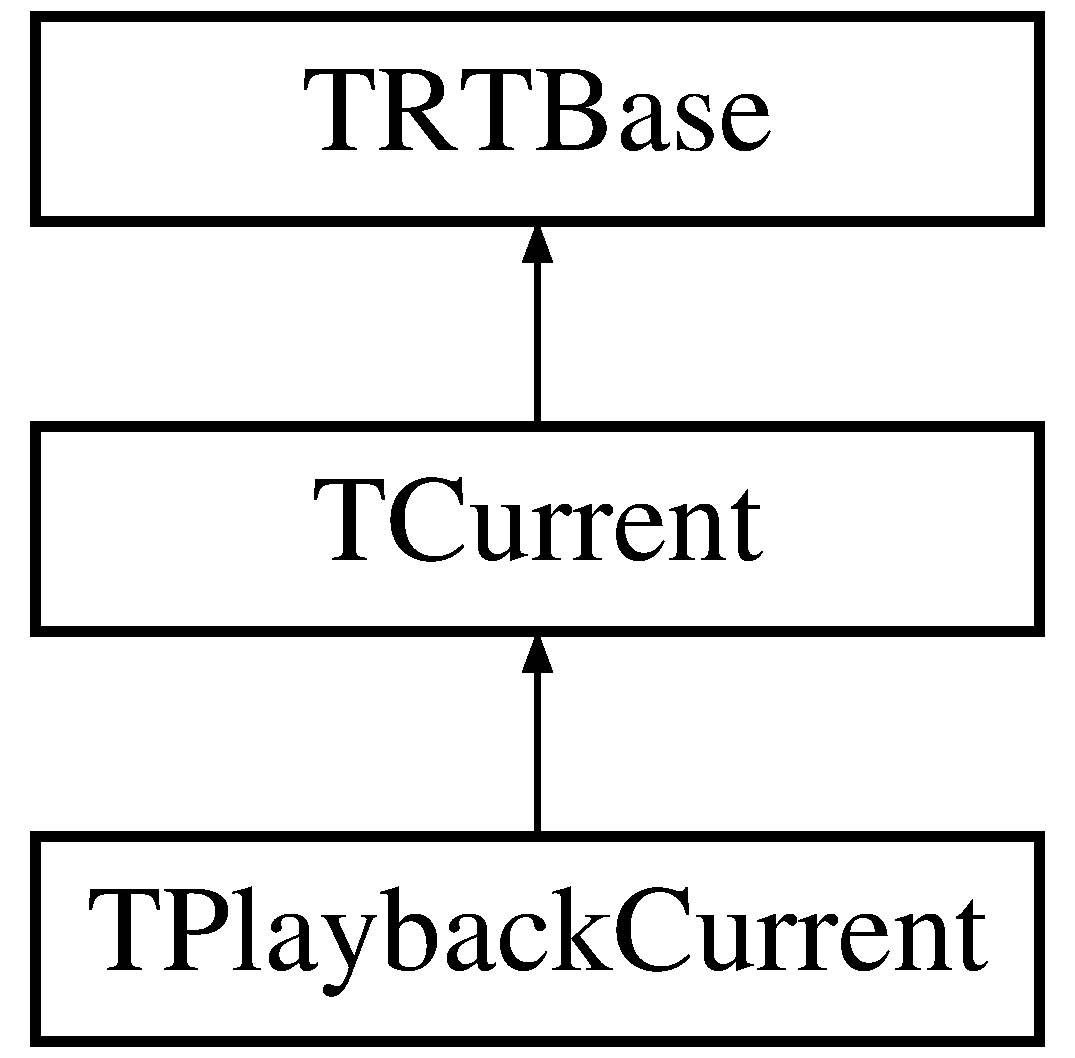
\includegraphics[height=3.000000cm]{class_t_playback_current}
\end{center}
\end{figure}
\subsection*{Public Member Functions}
\begin{DoxyCompactItemize}
\item 
\hypertarget{class_t_playback_current_ab502ccffe8273537850dab4790db79fd}{const double \+\_\+\+\_\+fastcall {\bfseries Gmax} ()}\label{class_t_playback_current_ab502ccffe8273537850dab4790db79fd}

\item 
\hypertarget{class_t_playback_current_a1f26dddfd2e5f46792d5112cb9e6ac67}{void \+\_\+\+\_\+fastcall {\bfseries Set\+Gmax} (double set)}\label{class_t_playback_current_a1f26dddfd2e5f46792d5112cb9e6ac67}

\item 
\hypertarget{class_t_playback_current_ab38a64219957c17687e2361def14324f}{virtual \hyperlink{class_t_playback_waveform}{T\+Playback\+Waveform} \\*
$\ast$const \+\_\+\+\_\+fastcall {\bfseries Get\+Playback\+Waveform} ()}\label{class_t_playback_current_ab38a64219957c17687e2361def14324f}

\item 
virtual void $\ast$const \+\_\+\+\_\+fastcall \hyperlink{class_t_playback_current_a28d0a767401ce8b53de441e83c6aae5c}{Get\+Edit\+Form} ()
\item 
\hypertarget{class_t_playback_current_aa5569339c8b6c425e67759b7be68d1d5}{virtual void \+\_\+\+\_\+fastcall \hyperlink{class_t_playback_current_aa5569339c8b6c425e67759b7be68d1d5}{Populate\+Edit\+Form} ()}\label{class_t_playback_current_aa5569339c8b6c425e67759b7be68d1d5}

\begin{DoxyCompactList}\small\item\em Interface for derived classes, called by G\+U\+I to update V\+C\+L form components. \end{DoxyCompactList}\item 
\hypertarget{class_t_playback_current_a0dad07f280f6bcdba5ac26675b0f4597}{virtual bool \+\_\+\+\_\+fastcall \hyperlink{class_t_playback_current_a0dad07f280f6bcdba5ac26675b0f4597}{Validate\+Edit\+Form} ()}\label{class_t_playback_current_a0dad07f280f6bcdba5ac26675b0f4597}

\begin{DoxyCompactList}\small\item\em Interface for derived classes, called by G\+U\+I to read V\+C\+L form values. \end{DoxyCompactList}\item 
virtual double \+\_\+\+\_\+fastcall \hyperlink{class_t_playback_current_abc30d522f008c19b885a09390f298a94}{Do\+Update} (double step, double Vkin, double Vdrv, std\+::vector$<$ double $>$ \&params)
\begin{DoxyCompactList}\small\item\em Override in derived classes to implement calculations. \end{DoxyCompactList}\item 
virtual bool \+\_\+\+\_\+fastcall \hyperlink{class_t_playback_current_a547567293caf240658b64a6f89d55737}{Initialize} (bool Reset)
\begin{DoxyCompactList}\small\item\em Sets Elapsed\+Time to zero. Must be called before first Update. \end{DoxyCompactList}\item 
const std\+::wstring \&\+\_\+\+\_\+fastcall \hyperlink{class_t_playback_current_aabc05c6ace3f33105e3c0645785cc38a}{Class\+Key} () const 
\begin{DoxyCompactList}\small\item\em Returns string used to register class with factory. \end{DoxyCompactList}\item 
\hypertarget{class_t_playback_current_aeaac39223d617d49edcc464a85744433}{\+\_\+\+\_\+fastcall \hyperlink{class_t_playback_current_aeaac39223d617d49edcc464a85744433}{T\+Playback\+Current} ()}\label{class_t_playback_current_aeaac39223d617d49edcc464a85744433}

\begin{DoxyCompactList}\small\item\em Default Constructor. \end{DoxyCompactList}\item 
\hypertarget{class_t_playback_current_af57f23f36e61849c8037809b1d98397d}{\+\_\+\+\_\+fastcall \hyperlink{class_t_playback_current_af57f23f36e61849c8037809b1d98397d}{T\+Playback\+Current} (\hyperlink{class_t_current_user}{T\+Current\+User} $\ast$owner, const std\+::wstring \&name)}\label{class_t_playback_current_af57f23f36e61849c8037809b1d98397d}

\begin{DoxyCompactList}\small\item\em Specialized Constructor 2 param. \end{DoxyCompactList}\item 
\hypertarget{class_t_playback_current_ab47f87894a2ebd8bce3338858dca7367}{\+\_\+\+\_\+fastcall \hyperlink{class_t_playback_current_ab47f87894a2ebd8bce3338858dca7367}{T\+Playback\+Current} (const std\+::wstring \&name)}\label{class_t_playback_current_ab47f87894a2ebd8bce3338858dca7367}

\begin{DoxyCompactList}\small\item\em Specialized Constructor 1 param. \end{DoxyCompactList}\item 
\hypertarget{class_t_playback_current_a4c38c5735ae6c69d88cab0daab923aec}{\+\_\+\+\_\+fastcall \hyperlink{class_t_playback_current_a4c38c5735ae6c69d88cab0daab923aec}{T\+Playback\+Current} (const \hyperlink{class_t_playback_current}{T\+Playback\+Current} \&source)}\label{class_t_playback_current_a4c38c5735ae6c69d88cab0daab923aec}

\begin{DoxyCompactList}\small\item\em copy constructor \end{DoxyCompactList}\item 
\hypertarget{class_t_playback_current_a24965d14280902d0f3ae98445dcef29f}{\hyperlink{class_t_playback_current}{T\+Playback\+Current} \& \hyperlink{class_t_playback_current_a24965d14280902d0f3ae98445dcef29f}{operator=} (const \hyperlink{class_t_playback_current}{T\+Playback\+Current} \&source)}\label{class_t_playback_current_a24965d14280902d0f3ae98445dcef29f}

\begin{DoxyCompactList}\small\item\em overloaded assignment operator \end{DoxyCompactList}\item 
\hypertarget{class_t_playback_current_a08245f2df509f42674f4c2a1eb5b6cf5}{virtual void \+\_\+\+\_\+fastcall \hyperlink{class_t_playback_current_a08245f2df509f42674f4c2a1eb5b6cf5}{Copy\+Params\+From} (const \hyperlink{class_t_current}{T\+Current} $\ast$const source)}\label{class_t_playback_current_a08245f2df509f42674f4c2a1eb5b6cf5}

\begin{DoxyCompactList}\small\item\em overloaded method for duplicating currents without complete assignment \end{DoxyCompactList}\end{DoxyCompactItemize}
\subsection*{Protected Member Functions}
\begin{DoxyCompactItemize}
\item 
\hypertarget{class_t_playback_current_a3404d1aae6418c9fad506bcbb785f0b9}{void const \+\_\+\+\_\+fastcall \hyperlink{class_t_playback_current_a3404d1aae6418c9fad506bcbb785f0b9}{Write\+To\+Stream} (ostream \&stream) const }\label{class_t_playback_current_a3404d1aae6418c9fad506bcbb785f0b9}

\begin{DoxyCompactList}\small\item\em Writes data members to a stream. \end{DoxyCompactList}\item 
\hypertarget{class_t_playback_current_a9f595f63d44ad217c268904cb6cc390c}{void const \+\_\+\+\_\+fastcall \hyperlink{class_t_playback_current_a9f595f63d44ad217c268904cb6cc390c}{Read\+From\+Stream} (istream \&stream)}\label{class_t_playback_current_a9f595f63d44ad217c268904cb6cc390c}

\begin{DoxyCompactList}\small\item\em Reads data members from a stream. \end{DoxyCompactList}\item 
const void \+\_\+\+\_\+fastcall \hyperlink{class_t_playback_current_acc4966648d397dfb5c368eef25249170}{Get\+Param\+Log\+Header} (std\+::vector$<$ std\+::string $>$ \&params) const 
\begin{DoxyCompactList}\small\item\em Supplies column names for parameter logging. \end{DoxyCompactList}\end{DoxyCompactItemize}
\subsection*{Friends}
\begin{DoxyCompactItemize}
\item 
\hypertarget{class_t_playback_current_ac98d07dd8f7b70e16ccb9a01abf56b9c}{class {\bfseries boost\+::serialization\+::access}}\label{class_t_playback_current_ac98d07dd8f7b70e16ccb9a01abf56b9c}

\end{DoxyCompactItemize}


\subsection{Detailed Description}
Implements a current for an electrical synapse. 

\begin{DoxyAuthor}{Author}
E. Brady Trexler $<$ebtrexler (at) gothamsci.\+com$>$, 2011 -\/ 2013 
\end{DoxyAuthor}


\subsection{Member Function Documentation}
\hypertarget{class_t_playback_current_aabc05c6ace3f33105e3c0645785cc38a}{\index{T\+Playback\+Current@{T\+Playback\+Current}!Class\+Key@{Class\+Key}}
\index{Class\+Key@{Class\+Key}!T\+Playback\+Current@{T\+Playback\+Current}}
\subsubsection[{Class\+Key}]{\setlength{\rightskip}{0pt plus 5cm}const std\+::wstring\& \+\_\+\+\_\+fastcall T\+Playback\+Current\+::\+Class\+Key (
\begin{DoxyParamCaption}
{}
\end{DoxyParamCaption}
) const\hspace{0.3cm}{\ttfamily [inline]}, {\ttfamily [virtual]}}}\label{class_t_playback_current_aabc05c6ace3f33105e3c0645785cc38a}


Returns string used to register class with factory. 

Users of class factories must also tell the class the key they used when registering the class. See factory.\+h 

Implements \hyperlink{class_t_r_t_base_a6083fd510cbcb00faa85e5934fc3c18e}{T\+R\+T\+Base}.

\hypertarget{class_t_playback_current_abc30d522f008c19b885a09390f298a94}{\index{T\+Playback\+Current@{T\+Playback\+Current}!Do\+Update@{Do\+Update}}
\index{Do\+Update@{Do\+Update}!T\+Playback\+Current@{T\+Playback\+Current}}
\subsubsection[{Do\+Update}]{\setlength{\rightskip}{0pt plus 5cm}virtual double \+\_\+\+\_\+fastcall T\+Playback\+Current\+::\+Do\+Update (
\begin{DoxyParamCaption}
\item[{double}]{step, }
\item[{double}]{Vkin, }
\item[{double}]{Vdrv, }
\item[{std\+::vector$<$ double $>$ \&}]{params}
\end{DoxyParamCaption}
)\hspace{0.3cm}{\ttfamily [inline]}, {\ttfamily [virtual]}}}\label{class_t_playback_current_abc30d522f008c19b885a09390f298a94}


Override in derived classes to implement calculations. 


\begin{DoxyParams}{Parameters}
{\em step} & = milliseconds passed since last call \\
\hline
{\em Vkin} & = voltage governing kinetics of conductance \\
\hline
{\em Vdrv} & = voltage governing ionic flow through conductance \\
\hline
{\em params} & = vector of calculated parameters for logging \\
\hline
\end{DoxyParams}


Implements \hyperlink{class_t_current_a36d89025eb424f6905fef945c9ae4fa7}{T\+Current}.

\hypertarget{class_t_playback_current_a28d0a767401ce8b53de441e83c6aae5c}{\index{T\+Playback\+Current@{T\+Playback\+Current}!Get\+Edit\+Form@{Get\+Edit\+Form}}
\index{Get\+Edit\+Form@{Get\+Edit\+Form}!T\+Playback\+Current@{T\+Playback\+Current}}
\subsubsection[{Get\+Edit\+Form}]{\setlength{\rightskip}{0pt plus 5cm}virtual void$\ast$ const \+\_\+\+\_\+fastcall T\+Playback\+Current\+::\+Get\+Edit\+Form (
\begin{DoxyParamCaption}
{}
\end{DoxyParamCaption}
)\hspace{0.3cm}{\ttfamily [inline]}, {\ttfamily [virtual]}}}\label{class_t_playback_current_a28d0a767401ce8b53de441e83c6aae5c}
Interface for derived classes, returns pointer to G\+U\+I object for editing members. Callers must cast pointer to the correct object. 

Implements \hyperlink{class_t_r_t_base_ab83e520005e20ee71f98f3e85e1ee6d4}{T\+R\+T\+Base}.

\hypertarget{class_t_playback_current_acc4966648d397dfb5c368eef25249170}{\index{T\+Playback\+Current@{T\+Playback\+Current}!Get\+Param\+Log\+Header@{Get\+Param\+Log\+Header}}
\index{Get\+Param\+Log\+Header@{Get\+Param\+Log\+Header}!T\+Playback\+Current@{T\+Playback\+Current}}
\subsubsection[{Get\+Param\+Log\+Header}]{\setlength{\rightskip}{0pt plus 5cm}const void \+\_\+\+\_\+fastcall T\+Playback\+Current\+::\+Get\+Param\+Log\+Header (
\begin{DoxyParamCaption}
\item[{std\+::vector$<$ std\+::string $>$ \&}]{params}
\end{DoxyParamCaption}
) const\hspace{0.3cm}{\ttfamily [inline]}, {\ttfamily [protected]}, {\ttfamily [virtual]}}}\label{class_t_playback_current_acc4966648d397dfb5c368eef25249170}


Supplies column names for parameter logging. 


\begin{DoxyParams}{Parameters}
{\em params} & = vector of parameter names for logging Override in derived classes to add their parameters to the header \\
\hline
\end{DoxyParams}


Implements \hyperlink{class_t_current_ab49cb51723efade5eec00fa78fad7ad8}{T\+Current}.

\hypertarget{class_t_playback_current_a547567293caf240658b64a6f89d55737}{\index{T\+Playback\+Current@{T\+Playback\+Current}!Initialize@{Initialize}}
\index{Initialize@{Initialize}!T\+Playback\+Current@{T\+Playback\+Current}}
\subsubsection[{Initialize}]{\setlength{\rightskip}{0pt plus 5cm}virtual bool \+\_\+\+\_\+fastcall T\+Playback\+Current\+::\+Initialize (
\begin{DoxyParamCaption}
\item[{bool}]{reset}
\end{DoxyParamCaption}
)\hspace{0.3cm}{\ttfamily [inline]}, {\ttfamily [virtual]}}}\label{class_t_playback_current_a547567293caf240658b64a6f89d55737}


Sets Elapsed\+Time to zero. Must be called before first Update. 


\begin{DoxyParams}{Parameters}
{\em reset} & = flag for derived classes \\
\hline
\end{DoxyParams}


Reimplemented from \hyperlink{class_t_current_a00c70d232ae85a9841d8d07e5770b7bd}{T\+Current}.



The documentation for this class was generated from the following file\+:\begin{DoxyCompactItemize}
\item 
G\+U\+I\+\_\+\+R\+T\+\_\+\+Edit\+\_\+\+Playback\+Current.\+cpp\end{DoxyCompactItemize}

\hypertarget{class_t_playback_current_form}{\section{T\+Playback\+Current\+Form Class Reference}
\label{class_t_playback_current_form}\index{T\+Playback\+Current\+Form@{T\+Playback\+Current\+Form}}
}
Inheritance diagram for T\+Playback\+Current\+Form\+:\begin{figure}[H]
\begin{center}
\leavevmode
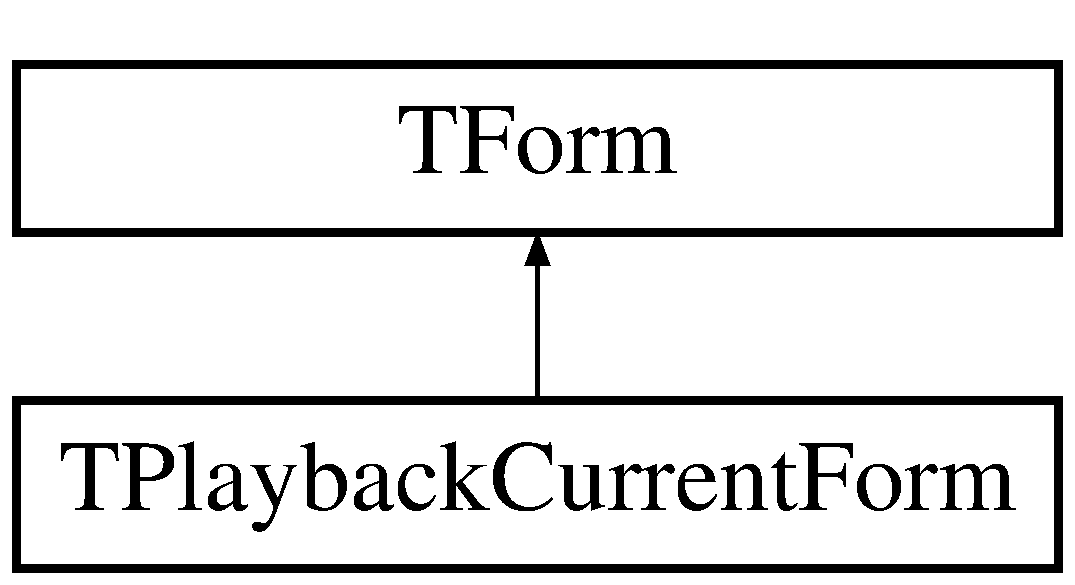
\includegraphics[height=2.000000cm]{class_t_playback_current_form}
\end{center}
\end{figure}
\subsection*{Public Member Functions}
\begin{DoxyCompactItemize}
\item 
\hypertarget{class_t_playback_current_form_a4563879147c51032379342cca0f409d1}{void \+\_\+\+\_\+fastcall {\bfseries Edit1\+Key\+Press} (T\+Object $\ast$Sender, wchar\+\_\+t \&Key)}\label{class_t_playback_current_form_a4563879147c51032379342cca0f409d1}

\item 
\hypertarget{class_t_playback_current_form_ae89bddd65a8d37d2f1a3930cb5536252}{\+\_\+\+\_\+fastcall {\bfseries T\+Playback\+Current\+Form} (T\+Component $\ast$Owner)}\label{class_t_playback_current_form_ae89bddd65a8d37d2f1a3930cb5536252}

\end{DoxyCompactItemize}
\subsection*{Public Attributes}
\begin{DoxyCompactItemize}
\item 
\hypertarget{class_t_playback_current_form_ac81385b006cbd257d398f1e703774fd4}{T\+Panel $\ast$ {\bfseries Panel6}}\label{class_t_playback_current_form_ac81385b006cbd257d398f1e703774fd4}

\item 
\hypertarget{class_t_playback_current_form_a9aaddaef01148e00d947cf87647bdc23}{T\+Label $\ast$ {\bfseries Label1}}\label{class_t_playback_current_form_a9aaddaef01148e00d947cf87647bdc23}

\item 
\hypertarget{class_t_playback_current_form_a684e46971011eb14d5ea31105332fe81}{T\+Label $\ast$ {\bfseries Label2}}\label{class_t_playback_current_form_a684e46971011eb14d5ea31105332fe81}

\item 
\hypertarget{class_t_playback_current_form_a5f3b2825d4839a454b4ce83c70f425e1}{T\+Label $\ast$ {\bfseries Label3}}\label{class_t_playback_current_form_a5f3b2825d4839a454b4ce83c70f425e1}

\item 
\hypertarget{class_t_playback_current_form_a2a2f35eb28d071d530c8fe09eee806a6}{T\+Label $\ast$ {\bfseries Label4}}\label{class_t_playback_current_form_a2a2f35eb28d071d530c8fe09eee806a6}

\item 
\hypertarget{class_t_playback_current_form_a2b565dc2acdf56ade58b4f5ea434cb08}{T\+Label $\ast$ {\bfseries Label6}}\label{class_t_playback_current_form_a2b565dc2acdf56ade58b4f5ea434cb08}

\item 
\hypertarget{class_t_playback_current_form_acb7308d0e31c1f5ea0f6a206421ef114}{T\+Edit $\ast$ {\bfseries Gmax\+Edit}}\label{class_t_playback_current_form_acb7308d0e31c1f5ea0f6a206421ef114}

\item 
\hypertarget{class_t_playback_current_form_a8783c6d8ae5e835d7bbf43eefbf5c933}{T\+Edit $\ast$ {\bfseries Erev\+Edit}}\label{class_t_playback_current_form_a8783c6d8ae5e835d7bbf43eefbf5c933}

\item 
\hypertarget{class_t_playback_current_form_a383affd09bf50600732d9294ab8c8922}{T\+Edit $\ast$ {\bfseries Gnoise\+Edit}}\label{class_t_playback_current_form_a383affd09bf50600732d9294ab8c8922}

\item 
\hypertarget{class_t_playback_current_form_a6f94d91a74249ddfefb4b047c9a233f5}{T\+Scroll\+Box $\ast$ {\bfseries Scroll\+Box1}}\label{class_t_playback_current_form_a6f94d91a74249ddfefb4b047c9a233f5}

\item 
\hypertarget{class_t_playback_current_form_ab555bf18508a4d124ae27fbe12d99563}{T\+Check\+Box $\ast$ {\bfseries Param\+Logging\+Check\+Box}}\label{class_t_playback_current_form_ab555bf18508a4d124ae27fbe12d99563}

\item 
\hypertarget{class_t_playback_current_form_acfb4a70754de5619c6b94c9fdb693cc5}{\hyperlink{class_t_playback_current}{T\+Playback\+Current} $\ast$ {\bfseries Playback\+Current}}\label{class_t_playback_current_form_acfb4a70754de5619c6b94c9fdb693cc5}

\end{DoxyCompactItemize}


The documentation for this class was generated from the following files\+:\begin{DoxyCompactItemize}
\item 
G\+U\+I\+\_\+\+R\+T\+\_\+\+Edit\+\_\+\+Playback\+Current.\+h\item 
G\+U\+I\+\_\+\+R\+T\+\_\+\+Edit\+\_\+\+Playback\+Current.\+cpp\end{DoxyCompactItemize}

\hypertarget{class_t_playback_electrode}{\section{T\+Playback\+Electrode Class Reference}
\label{class_t_playback_electrode}\index{T\+Playback\+Electrode@{T\+Playback\+Electrode}}
}


Derived class that implements an electrode that plays back pre-\/recorded waveform as n\+A.  


Inheritance diagram for T\+Playback\+Electrode\+:\begin{figure}[H]
\begin{center}
\leavevmode
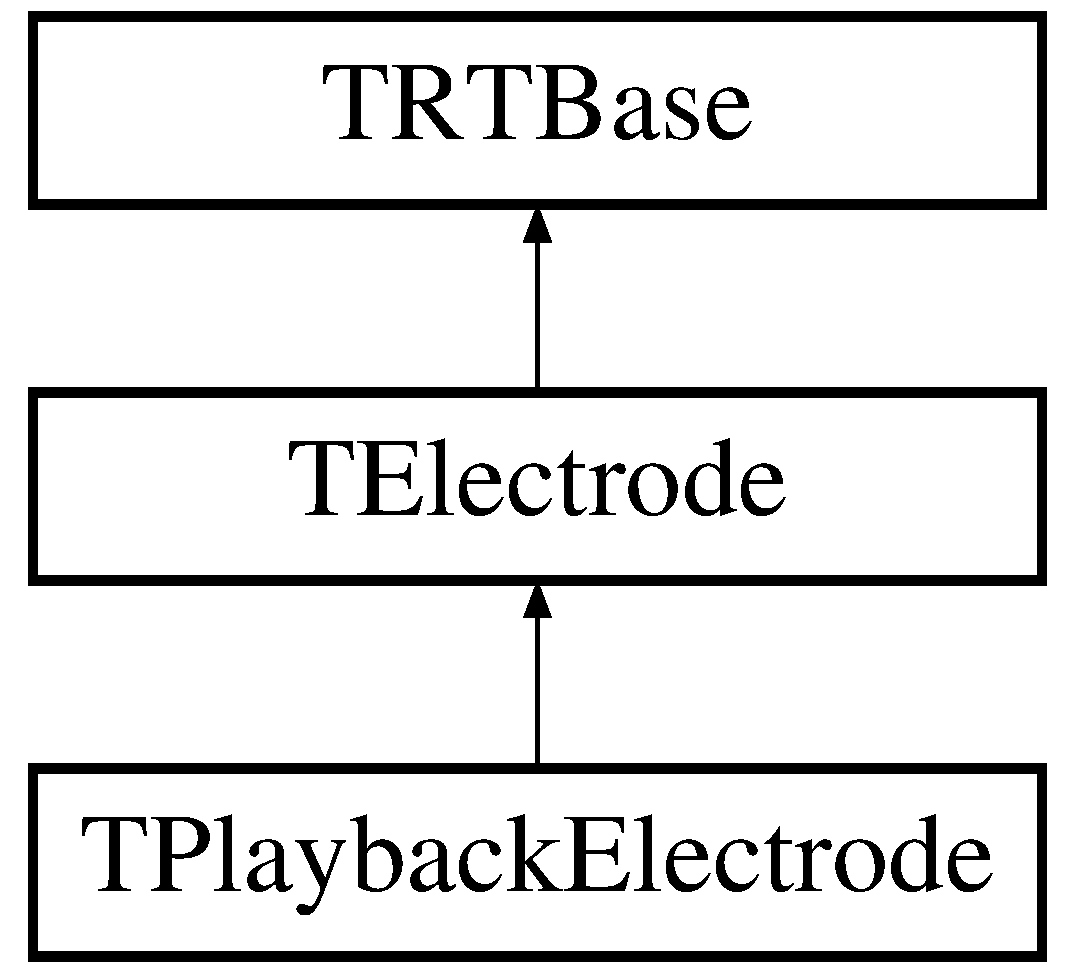
\includegraphics[height=3.000000cm]{class_t_playback_electrode}
\end{center}
\end{figure}
\subsection*{Public Member Functions}
\begin{DoxyCompactItemize}
\item 
\hypertarget{class_t_playback_electrode_a9a701d62d133f7328f80d5cda6f41704}{\+\_\+\+\_\+fastcall {\bfseries T\+Playback\+Electrode} (\hyperlink{class_t_cell}{T\+Cell} $\ast$const owner, const std\+::wstring \&name)}\label{class_t_playback_electrode_a9a701d62d133f7328f80d5cda6f41704}

\item 
\hypertarget{class_t_playback_electrode_aa6bc9934b13a28827b1e03ae92e9e3ff}{virtual \hyperlink{class_t_playback_waveform}{T\+Playback\+Waveform} \\*
$\ast$const \+\_\+\+\_\+fastcall {\bfseries Get\+Playback\+Waveform} ()}\label{class_t_playback_electrode_aa6bc9934b13a28827b1e03ae92e9e3ff}

\item 
\hypertarget{class_t_playback_electrode_a1d114194553aca06068cc828b8d791ee}{virtual double \+\_\+\+\_\+fastcall \hyperlink{class_t_playback_electrode_a1d114194553aca06068cc828b8d791ee}{Do\+Update} (double step)}\label{class_t_playback_electrode_a1d114194553aca06068cc828b8d791ee}

\begin{DoxyCompactList}\small\item\em Calculates current to inject, must override. \end{DoxyCompactList}\item 
\hypertarget{class_t_playback_electrode_a580e65eece4114789fe39f6d7a1cf689}{bool \+\_\+\+\_\+fastcall \hyperlink{class_t_playback_electrode_a580e65eece4114789fe39f6d7a1cf689}{Initialize} (bool Reset)}\label{class_t_playback_electrode_a580e65eece4114789fe39f6d7a1cf689}

\begin{DoxyCompactList}\small\item\em Must override but can call default implementation \hyperlink{class_t_electrode_a5f5711cfc03619d470acbe5669e59930}{T\+Electrode\+::\+Initialize()};. \end{DoxyCompactList}\item 
virtual void $\ast$const \+\_\+\+\_\+fastcall \hyperlink{class_t_playback_electrode_af870739aeec24862ed6333dc453951a1}{Get\+Edit\+Form} ()
\item 
\hypertarget{class_t_playback_electrode_af7362654435567684bc94fd02cebc5e1}{virtual void \+\_\+\+\_\+fastcall \hyperlink{class_t_playback_electrode_af7362654435567684bc94fd02cebc5e1}{Populate\+Edit\+Form} ()}\label{class_t_playback_electrode_af7362654435567684bc94fd02cebc5e1}

\begin{DoxyCompactList}\small\item\em Interface for derived classes, called by G\+U\+I to update V\+C\+L form components. \end{DoxyCompactList}\item 
\hypertarget{class_t_playback_electrode_a0d5e4e5828b7c9e877eaae2228ac219f}{virtual bool \+\_\+\+\_\+fastcall \hyperlink{class_t_playback_electrode_a0d5e4e5828b7c9e877eaae2228ac219f}{Validate\+Edit\+Form} ()}\label{class_t_playback_electrode_a0d5e4e5828b7c9e877eaae2228ac219f}

\begin{DoxyCompactList}\small\item\em Interface for derived classes, called by G\+U\+I to read V\+C\+L form values. \end{DoxyCompactList}\item 
const std\+::wstring \&\+\_\+\+\_\+fastcall \hyperlink{class_t_playback_electrode_ab1174a8ccda8d316130a899471341374}{Class\+Key} () const 
\begin{DoxyCompactList}\small\item\em Returns string used to register class with factory. \end{DoxyCompactList}\item 
\hypertarget{class_t_playback_electrode_a4d166b8df4a0f7798113c03bd804c2d7}{virtual const \hyperlink{class_t_current}{T\+Current} $\ast$\+\_\+\+\_\+fastcall \hyperlink{class_t_playback_electrode_a4d166b8df4a0f7798113c03bd804c2d7}{Add\+Current} (\hyperlink{class_t_current}{T\+Current} $\ast$const c, \hyperlink{class_t_cell}{T\+Cell} $\ast$cell=N\+U\+L\+L)}\label{class_t_playback_electrode_a4d166b8df4a0f7798113c03bd804c2d7}

\begin{DoxyCompactList}\small\item\em Overrides and disables adding a \hyperlink{class_t_current}{T\+Current} $\ast$ to the array of Currents. \end{DoxyCompactList}\item 
\hypertarget{class_t_playback_electrode_a051024e0d384e288ee2f6420aba34568}{virtual const \hyperlink{class_t_electrode}{T\+Electrode} \\*
$\ast$\+\_\+\+\_\+fastcall \hyperlink{class_t_playback_electrode_a051024e0d384e288ee2f6420aba34568}{Add\+Electrode} (\hyperlink{class_t_electrode}{T\+Electrode} $\ast$e)}\label{class_t_playback_electrode_a051024e0d384e288ee2f6420aba34568}

\begin{DoxyCompactList}\small\item\em Overrides and disables adding a \hyperlink{class_t_electrode}{T\+Electrode} $\ast$ to the array of Electrodes. \end{DoxyCompactList}\end{DoxyCompactItemize}
\subsection*{Protected Member Functions}
\begin{DoxyCompactItemize}
\item 
\hypertarget{class_t_playback_electrode_a1babab6ab1431872259c8dc48c916919}{virtual void const \+\_\+\+\_\+fastcall \hyperlink{class_t_playback_electrode_a1babab6ab1431872259c8dc48c916919}{Write\+To\+Stream} (ostream \&stream) const }\label{class_t_playback_electrode_a1babab6ab1431872259c8dc48c916919}

\begin{DoxyCompactList}\small\item\em pure virtual function for derived classes to write to a stream \end{DoxyCompactList}\item 
\hypertarget{class_t_playback_electrode_ab022309471d8430178d9569dfc0139bc}{virtual void const \+\_\+\+\_\+fastcall \hyperlink{class_t_playback_electrode_ab022309471d8430178d9569dfc0139bc}{Read\+From\+Stream} (istream \&stream)}\label{class_t_playback_electrode_ab022309471d8430178d9569dfc0139bc}

\begin{DoxyCompactList}\small\item\em pure virtual function for derived classes to read from a stream \end{DoxyCompactList}\end{DoxyCompactItemize}
\subsection*{Friends}
\begin{DoxyCompactItemize}
\item 
\hypertarget{class_t_playback_electrode_ac98d07dd8f7b70e16ccb9a01abf56b9c}{class \hyperlink{class_t_playback_electrode_ac98d07dd8f7b70e16ccb9a01abf56b9c}{boost\+::serialization\+::access}}\label{class_t_playback_electrode_ac98d07dd8f7b70e16ccb9a01abf56b9c}

\begin{DoxyCompactList}\small\item\em Required for serialization and saving networks to disk. \end{DoxyCompactList}\end{DoxyCompactItemize}


\subsection{Detailed Description}
Derived class that implements an electrode that plays back pre-\/recorded waveform as n\+A. 

Gains and offset alter waveform. Appropriate methods are overridden.

\begin{DoxyAuthor}{Author}
E. Brady Trexler $<$ebtrexler (at) gothamsci.\+com$>$, 2011 -\/ 2013 
\end{DoxyAuthor}


\subsection{Member Function Documentation}
\hypertarget{class_t_playback_electrode_ab1174a8ccda8d316130a899471341374}{\index{T\+Playback\+Electrode@{T\+Playback\+Electrode}!Class\+Key@{Class\+Key}}
\index{Class\+Key@{Class\+Key}!T\+Playback\+Electrode@{T\+Playback\+Electrode}}
\subsubsection[{Class\+Key}]{\setlength{\rightskip}{0pt plus 5cm}const std\+::wstring\& \+\_\+\+\_\+fastcall T\+Playback\+Electrode\+::\+Class\+Key (
\begin{DoxyParamCaption}
{}
\end{DoxyParamCaption}
) const\hspace{0.3cm}{\ttfamily [inline]}, {\ttfamily [virtual]}}}\label{class_t_playback_electrode_ab1174a8ccda8d316130a899471341374}


Returns string used to register class with factory. 

Users of class factories must also tell the class the key they used when registering the class. See factory.\+h 

Implements \hyperlink{class_t_r_t_base_a6083fd510cbcb00faa85e5934fc3c18e}{T\+R\+T\+Base}.

\hypertarget{class_t_playback_electrode_af870739aeec24862ed6333dc453951a1}{\index{T\+Playback\+Electrode@{T\+Playback\+Electrode}!Get\+Edit\+Form@{Get\+Edit\+Form}}
\index{Get\+Edit\+Form@{Get\+Edit\+Form}!T\+Playback\+Electrode@{T\+Playback\+Electrode}}
\subsubsection[{Get\+Edit\+Form}]{\setlength{\rightskip}{0pt plus 5cm}virtual void$\ast$ const \+\_\+\+\_\+fastcall T\+Playback\+Electrode\+::\+Get\+Edit\+Form (
\begin{DoxyParamCaption}
{}
\end{DoxyParamCaption}
)\hspace{0.3cm}{\ttfamily [inline]}, {\ttfamily [virtual]}}}\label{class_t_playback_electrode_af870739aeec24862ed6333dc453951a1}
Interface for derived classes, returns pointer to G\+U\+I object for editing members. Callers must cast pointer to the correct object. 

Implements \hyperlink{class_t_r_t_base_ab83e520005e20ee71f98f3e85e1ee6d4}{T\+R\+T\+Base}.



The documentation for this class was generated from the following file\+:\begin{DoxyCompactItemize}
\item 
G\+U\+I\+\_\+\+R\+T\+\_\+\+Edit\+\_\+\+Playback\+Electrode.\+cpp\end{DoxyCompactItemize}

\hypertarget{class_t_playback_electrode_form}{\section{T\+Playback\+Electrode\+Form Class Reference}
\label{class_t_playback_electrode_form}\index{T\+Playback\+Electrode\+Form@{T\+Playback\+Electrode\+Form}}
}


G\+U\+I Editor for \hyperlink{class_t_playback_electrode}{T\+Playback\+Electrode}.  




{\ttfamily \#include $<$G\+U\+I\+\_\+\+R\+T\+\_\+\+Edit\+\_\+\+Playback\+Electrode.\+h$>$}

Inheritance diagram for T\+Playback\+Electrode\+Form\+:\begin{figure}[H]
\begin{center}
\leavevmode
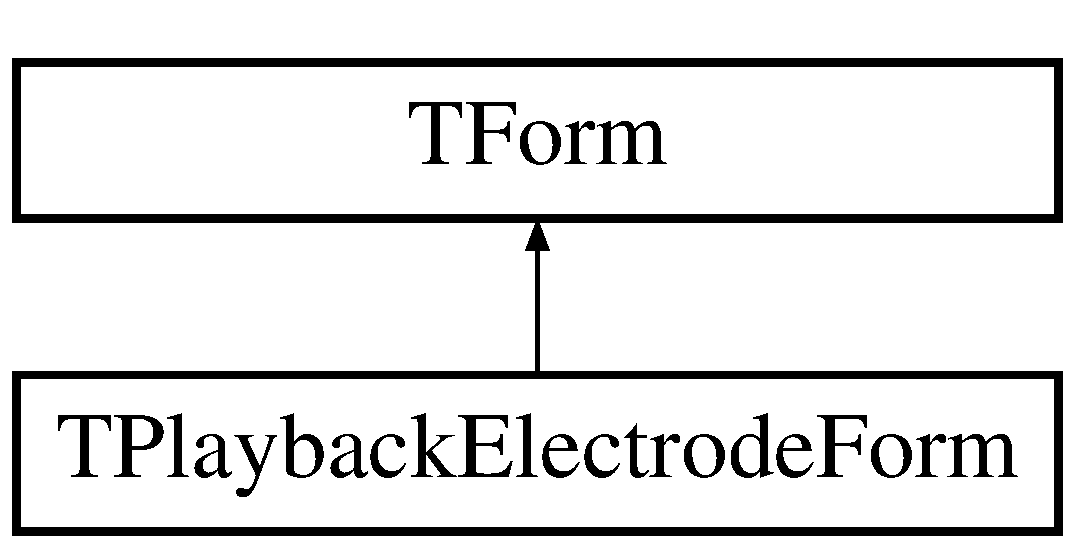
\includegraphics[height=2.000000cm]{class_t_playback_electrode_form}
\end{center}
\end{figure}
\subsection*{Public Member Functions}
\begin{DoxyCompactItemize}
\item 
\hypertarget{class_t_playback_electrode_form_ae6af233c1a9cae8ba4da4fbcd49a8409}{\+\_\+\+\_\+fastcall {\bfseries T\+Playback\+Electrode\+Form} (T\+Component $\ast$Owner)}\label{class_t_playback_electrode_form_ae6af233c1a9cae8ba4da4fbcd49a8409}

\end{DoxyCompactItemize}
\subsection*{Public Attributes}
\begin{DoxyCompactItemize}
\item 
\hypertarget{class_t_playback_electrode_form_a310a9dd051af08558ddcc0b40d49a1c9}{T\+Open\+Dialog $\ast$ {\bfseries Open\+Dialog1}}\label{class_t_playback_electrode_form_a310a9dd051af08558ddcc0b40d49a1c9}

\item 
\hypertarget{class_t_playback_electrode_form_a8154a99f806a5ab123d4487a446bed30}{T\+Image\+List $\ast$ {\bfseries Image\+List1}}\label{class_t_playback_electrode_form_a8154a99f806a5ab123d4487a446bed30}

\item 
\hypertarget{class_t_playback_electrode_form_abd05dd8c1356a58f30ed1cc95a8370dd}{T\+P\+L\+O\+T\+Panel $\ast$ {\bfseries P\+L\+O\+T\+Panel1}}\label{class_t_playback_electrode_form_abd05dd8c1356a58f30ed1cc95a8370dd}

\item 
\hypertarget{class_t_playback_electrode_form_a56de6957a8a69c6d362e191e7e5e3d16}{T\+Label $\ast$ {\bfseries Label1}}\label{class_t_playback_electrode_form_a56de6957a8a69c6d362e191e7e5e3d16}

\item 
\hypertarget{class_t_playback_electrode_form_a4a79b78e602547e327aaa2ee8d712d37}{T\+Label $\ast$ {\bfseries File\+Label}}\label{class_t_playback_electrode_form_a4a79b78e602547e327aaa2ee8d712d37}

\item 
\hypertarget{class_t_playback_electrode_form_a038fb65af149a115d77b111a0a21220d}{T\+Bit\+Btn $\ast$ {\bfseries Browse\+Bit\+Btn}}\label{class_t_playback_electrode_form_a038fb65af149a115d77b111a0a21220d}

\item 
\hypertarget{class_t_playback_electrode_form_a0ea74498e6fee2b9a20833dedb9217df}{T\+Label $\ast$ {\bfseries Label2}}\label{class_t_playback_electrode_form_a0ea74498e6fee2b9a20833dedb9217df}

\item 
\hypertarget{class_t_playback_electrode_form_addbe27279018aa91697231fcf43b67b4}{T\+Combo\+Box $\ast$ {\bfseries Channel\+Combo\+Box}}\label{class_t_playback_electrode_form_addbe27279018aa91697231fcf43b67b4}

\item 
\hypertarget{class_t_playback_electrode_form_a046dbbfc5479ca0bb7716c5d8fe8fb0b}{T\+Label $\ast$ {\bfseries Label3}}\label{class_t_playback_electrode_form_a046dbbfc5479ca0bb7716c5d8fe8fb0b}

\item 
\hypertarget{class_t_playback_electrode_form_a4fdf4a3d5b24cef5c31306b104c54e5b}{T\+Edit $\ast$ {\bfseries Convertn\+A\+Edit}}\label{class_t_playback_electrode_form_a4fdf4a3d5b24cef5c31306b104c54e5b}

\item 
\hypertarget{class_t_playback_electrode_form_a6430163c6fafddc11488fec3ec66adde}{T\+Label $\ast$ {\bfseries Label4}}\label{class_t_playback_electrode_form_a6430163c6fafddc11488fec3ec66adde}

\item 
\hypertarget{class_t_playback_electrode_form_a636a544c3634fe39f7e0e978fac063c5}{T\+Label $\ast$ {\bfseries Sample\+Period\+Label}}\label{class_t_playback_electrode_form_a636a544c3634fe39f7e0e978fac063c5}

\item 
\hypertarget{class_t_playback_electrode_form_aab4f1a8edd146a4e16f2bbe290b797a7}{\hyperlink{class_t_playback_electrode}{T\+Playback\+Electrode} $\ast$ {\bfseries Electrode}}\label{class_t_playback_electrode_form_aab4f1a8edd146a4e16f2bbe290b797a7}

\end{DoxyCompactItemize}


\subsection{Detailed Description}
G\+U\+I Editor for \hyperlink{class_t_playback_electrode}{T\+Playback\+Electrode}. 

\begin{DoxyAuthor}{Author}
E. Brady Trexler $<$ebtrexler (at) gothamsci.\+com$>$, 2011 -\/ 2013 
\end{DoxyAuthor}


The documentation for this class was generated from the following files\+:\begin{DoxyCompactItemize}
\item 
G\+U\+I\+\_\+\+R\+T\+\_\+\+Edit\+\_\+\+Playback\+Electrode.\+h\item 
G\+U\+I\+\_\+\+R\+T\+\_\+\+Edit\+\_\+\+Playback\+Electrode.\+cpp\end{DoxyCompactItemize}

\hypertarget{class_t_playback_waveform}{\section{T\+Playback\+Waveform Class Reference}
\label{class_t_playback_waveform}\index{T\+Playback\+Waveform@{T\+Playback\+Waveform}}
}


Derived class that loads and stores pre-\/recorded waveforms.  




{\ttfamily \#include $<$G\+U\+I\+\_\+\+Playback\+Waveform.\+h$>$}

Inheritance diagram for T\+Playback\+Waveform\+:\begin{figure}[H]
\begin{center}
\leavevmode
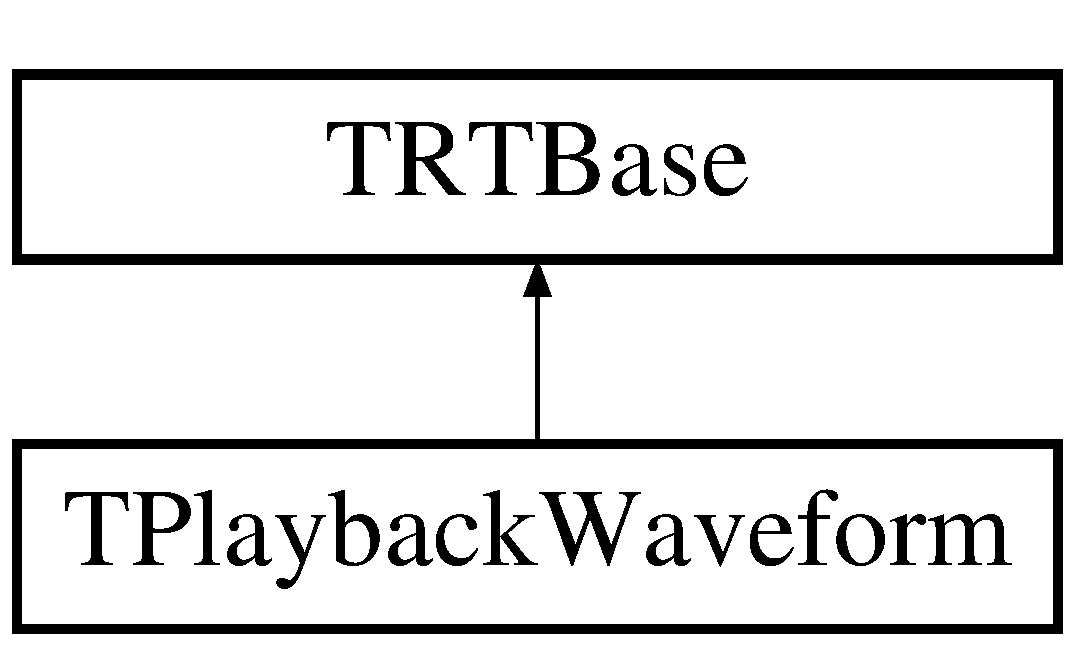
\includegraphics[height=2.000000cm]{class_t_playback_waveform}
\end{center}
\end{figure}
\subsection*{Public Member Functions}
\begin{DoxyCompactItemize}
\item 
\hypertarget{class_t_playback_waveform_aa7c520646204d2c8287fa19096c99172}{\+\_\+\+\_\+fastcall {\bfseries T\+Playback\+Waveform} (const std\+::wstring \&name)}\label{class_t_playback_waveform_aa7c520646204d2c8287fa19096c99172}

\item 
\hypertarget{class_t_playback_waveform_a5aed28140f1fda7df687a83899589e41}{void \+\_\+\+\_\+fastcall {\bfseries Update\+Plot} ()}\label{class_t_playback_waveform_a5aed28140f1fda7df687a83899589e41}

\item 
\hypertarget{class_t_playback_waveform_a3be6b2c54ae80df5df54ac0b1da24d5d}{void \+\_\+\+\_\+fastcall {\bfseries Set\+File\+Name} (std\+::wstring fname)}\label{class_t_playback_waveform_a3be6b2c54ae80df5df54ac0b1da24d5d}

\item 
\hypertarget{class_t_playback_waveform_ae4e5af610750ab71d5ba0beffa2132e4}{void \+\_\+\+\_\+fastcall {\bfseries Set\+Channel} (int channel)}\label{class_t_playback_waveform_ae4e5af610750ab71d5ba0beffa2132e4}

\item 
\hypertarget{class_t_playback_waveform_a277b2f5e1baa0bcc1ae7c6f5b09323a3}{void \+\_\+\+\_\+fastcall {\bfseries Set\+Scale\+Factor} (double factor)}\label{class_t_playback_waveform_a277b2f5e1baa0bcc1ae7c6f5b09323a3}

\item 
\hypertarget{class_t_playback_waveform_aa2fc72ac8982dee01460340c8f837659}{void \+\_\+\+\_\+fastcall {\bfseries Set\+Offset} (double offset)}\label{class_t_playback_waveform_aa2fc72ac8982dee01460340c8f837659}

\item 
\hypertarget{class_t_playback_waveform_a5cbec07e9ce6a16b49e45a31c8a65b41}{void \+\_\+\+\_\+fastcall {\bfseries Set\+Sample\+Rate} (double rate)}\label{class_t_playback_waveform_a5cbec07e9ce6a16b49e45a31c8a65b41}

\item 
\hypertarget{class_t_playback_waveform_a8d869607c56e5f11f32733d192d4a43d}{void \+\_\+\+\_\+fastcall {\bfseries Set\+Wfm\+Duration} (double time)}\label{class_t_playback_waveform_a8d869607c56e5f11f32733d192d4a43d}

\item 
\hypertarget{class_t_playback_waveform_ad16e3e03e6630c0bb9c6e7cf8546cb85}{void \+\_\+\+\_\+fastcall {\bfseries Set\+Units} (std\+::wstring units)}\label{class_t_playback_waveform_ad16e3e03e6630c0bb9c6e7cf8546cb85}

\item 
\hypertarget{class_t_playback_waveform_a8c06266cf29d6475b709d6b1561790e0}{void \+\_\+\+\_\+fastcall {\bfseries Set\+T\+X\+T\+Time\+Column} (bool set)}\label{class_t_playback_waveform_a8c06266cf29d6475b709d6b1561790e0}

\item 
\hypertarget{class_t_playback_waveform_a814796ce7c81ce34e270a78e9d3b2af0}{void \+\_\+\+\_\+fastcall {\bfseries Set\+T\+X\+T\+Header\+Row} (bool set)}\label{class_t_playback_waveform_a814796ce7c81ce34e270a78e9d3b2af0}

\item 
\hypertarget{class_t_playback_waveform_a1355cc4ffe882d3e708f14bd7689ff7b}{void \+\_\+\+\_\+fastcall {\bfseries Set\+Repeat\+Number} (int num)}\label{class_t_playback_waveform_a1355cc4ffe882d3e708f14bd7689ff7b}

\item 
\hypertarget{class_t_playback_waveform_af40738538a616b75abf1399fc10d86b0}{void \+\_\+\+\_\+fastcall {\bfseries Set\+Concatenate\+Episodes} (bool set)}\label{class_t_playback_waveform_af40738538a616b75abf1399fc10d86b0}

\item 
\hypertarget{class_t_playback_waveform_a55b1b7f1ac416198977043b0a5592199}{void \+\_\+\+\_\+fastcall {\bfseries Set\+Delay\+Before\+Repeat} (double delay)}\label{class_t_playback_waveform_a55b1b7f1ac416198977043b0a5592199}

\item 
\hypertarget{class_t_playback_waveform_a86a3d5aef61514ab4626b32705bae62f}{double \+\_\+\+\_\+fastcall {\bfseries Evaluate\+At\+Next} (double step)}\label{class_t_playback_waveform_a86a3d5aef61514ab4626b32705bae62f}

\item 
\hypertarget{class_t_playback_waveform_a825e2316f083038e26a5750ee49cfcec}{double \+\_\+\+\_\+fastcall {\bfseries Get\+File\+Duration} ()}\label{class_t_playback_waveform_a825e2316f083038e26a5750ee49cfcec}

\item 
\hypertarget{class_t_playback_waveform_a2a7ddf113350a906737d6e19d546bce1}{double \+\_\+\+\_\+fastcall {\bfseries Get\+Playback\+Rate} ()}\label{class_t_playback_waveform_a2a7ddf113350a906737d6e19d546bce1}

\item 
\hypertarget{class_t_playback_waveform_ad7a57b795e3c7b2c9f4f48e43db97c0c}{int \+\_\+\+\_\+fastcall {\bfseries Get\+Num\+Episodes} ()}\label{class_t_playback_waveform_ad7a57b795e3c7b2c9f4f48e43db97c0c}

\item 
\hypertarget{class_t_playback_waveform_ae42334d0a3445961bb4142ee0c5bd1e8}{double \+\_\+\+\_\+fastcall {\bfseries Get\+Episode\+Spacing} ()}\label{class_t_playback_waveform_ae42334d0a3445961bb4142ee0c5bd1e8}

\item 
\hypertarget{class_t_playback_waveform_aef1419913b7306a5e8d7085d20357531}{const std\+::vector$<$ std\+::string $>$\\*
 \&\+\_\+\+\_\+fastcall {\bfseries Get\+Channel\+Names} ()}\label{class_t_playback_waveform_aef1419913b7306a5e8d7085d20357531}

\item 
\hypertarget{class_t_playback_waveform_af5c6e558e8067717a6471d1fe99f407f}{const std\+::wstring \&\+\_\+\+\_\+fastcall {\bfseries Get\+File\+Name} ()}\label{class_t_playback_waveform_af5c6e558e8067717a6471d1fe99f407f}

\item 
\hypertarget{class_t_playback_waveform_aea3464377aa910def8d269b4e9bd9aef}{long \+\_\+\+\_\+fastcall {\bfseries Get\+Num\+Points} ()}\label{class_t_playback_waveform_aea3464377aa910def8d269b4e9bd9aef}

\item 
\hypertarget{class_t_playback_waveform_ad2464d9af56c3658a07b98d7de93d33f}{int \+\_\+\+\_\+fastcall {\bfseries Get\+Num\+Chans} ()}\label{class_t_playback_waveform_ad2464d9af56c3658a07b98d7de93d33f}

\item 
\hypertarget{class_t_playback_waveform_ae85f6e9771b93bbdc6f1a667520ace3d}{bool \+\_\+\+\_\+fastcall {\bfseries Get\+Channel\+Data} (int chan, std\+::vector$<$ double $>$ \&chandata)}\label{class_t_playback_waveform_ae85f6e9771b93bbdc6f1a667520ace3d}

\item 
\hypertarget{class_t_playback_waveform_aa717d45b40b6e85e914f1e9fdcfbe5b9}{bool \+\_\+\+\_\+fastcall \hyperlink{class_t_playback_waveform_aa717d45b40b6e85e914f1e9fdcfbe5b9}{Initialize} (bool Reset)}\label{class_t_playback_waveform_aa717d45b40b6e85e914f1e9fdcfbe5b9}

\begin{DoxyCompactList}\small\item\em pure virtual function for resetting before networking run \end{DoxyCompactList}\item 
const std\+::wstring \&\+\_\+\+\_\+fastcall \hyperlink{class_t_playback_waveform_ad5bb30fcf319f49b1119881d857262fa}{Class\+Key} () const 
\begin{DoxyCompactList}\small\item\em Returns string used to register class with factory. \end{DoxyCompactList}\item 
virtual void $\ast$const \+\_\+\+\_\+fastcall \hyperlink{class_t_playback_waveform_a1fcb2c8d237e2418080fdefeb3e13f73}{Get\+Edit\+Form} ()
\item 
\hypertarget{class_t_playback_waveform_ab97a5f8d756b7771fc58a6ac068c214c}{virtual void \+\_\+\+\_\+fastcall \hyperlink{class_t_playback_waveform_ab97a5f8d756b7771fc58a6ac068c214c}{Populate\+Edit\+Form} ()}\label{class_t_playback_waveform_ab97a5f8d756b7771fc58a6ac068c214c}

\begin{DoxyCompactList}\small\item\em Interface for derived classes, called by G\+U\+I to update V\+C\+L form components. \end{DoxyCompactList}\item 
\hypertarget{class_t_playback_waveform_a037a040342eb225bbedc6bb746827b58}{virtual bool \+\_\+\+\_\+fastcall \hyperlink{class_t_playback_waveform_a037a040342eb225bbedc6bb746827b58}{Validate\+Edit\+Form} ()}\label{class_t_playback_waveform_a037a040342eb225bbedc6bb746827b58}

\begin{DoxyCompactList}\small\item\em Interface for derived classes, called by G\+U\+I to read V\+C\+L form values. \end{DoxyCompactList}\end{DoxyCompactItemize}
\subsection*{Protected Member Functions}
\begin{DoxyCompactItemize}
\item 
\hypertarget{class_t_playback_waveform_a6f0b616de0f97ac7f80ad48525e54a37}{virtual void const \+\_\+\+\_\+fastcall \hyperlink{class_t_playback_waveform_a6f0b616de0f97ac7f80ad48525e54a37}{Write\+To\+Stream} (ostream \&stream) const }\label{class_t_playback_waveform_a6f0b616de0f97ac7f80ad48525e54a37}

\begin{DoxyCompactList}\small\item\em pure virtual function for derived classes to write to a stream \end{DoxyCompactList}\item 
\hypertarget{class_t_playback_waveform_a8ce9222064814e1b23ebd21de82cc954}{virtual void const \+\_\+\+\_\+fastcall \hyperlink{class_t_playback_waveform_a8ce9222064814e1b23ebd21de82cc954}{Read\+From\+Stream} (istream \&stream)}\label{class_t_playback_waveform_a8ce9222064814e1b23ebd21de82cc954}

\begin{DoxyCompactList}\small\item\em pure virtual function for derived classes to read from a stream \end{DoxyCompactList}\item 
bool \+\_\+\+\_\+fastcall \hyperlink{class_t_playback_waveform_a1ed2634cdd5bf2370264547b7ee3a418}{Get\+File\+Info} ()
\begin{DoxyCompactList}\small\item\em Opens a file and get available channels and sample rate. \end{DoxyCompactList}\item 
\hypertarget{class_t_playback_waveform_a5465ca76a723e65f75cb1aed51d98ca5}{bool \+\_\+\+\_\+fastcall {\bfseries Get\+File\+Info\+A\+B\+F} ()}\label{class_t_playback_waveform_a5465ca76a723e65f75cb1aed51d98ca5}

\item 
\hypertarget{class_t_playback_waveform_a9ecf34487481726e165425ce08abc17b}{bool \+\_\+\+\_\+fastcall {\bfseries Get\+File\+Info\+Spike2} ()}\label{class_t_playback_waveform_a9ecf34487481726e165425ce08abc17b}

\item 
\hypertarget{class_t_playback_waveform_ae3b16998b0e8ff6da84c4c8765682128}{bool \+\_\+\+\_\+fastcall {\bfseries Get\+File\+Info\+T\+X\+T} ()}\label{class_t_playback_waveform_ae3b16998b0e8ff6da84c4c8765682128}

\item 
\hypertarget{class_t_playback_waveform_a2e58a7db9903e5acba89276c18989650}{bool \+\_\+\+\_\+fastcall \hyperlink{class_t_playback_waveform_a2e58a7db9903e5acba89276c18989650}{Read\+Channel} ()}\label{class_t_playback_waveform_a2e58a7db9903e5acba89276c18989650}

\begin{DoxyCompactList}\small\item\em Opens a file and reads in selected channel. \end{DoxyCompactList}\item 
\hypertarget{class_t_playback_waveform_a84ad70c7b8ced225181e0c5df4be8bf8}{bool \+\_\+\+\_\+fastcall {\bfseries Read\+A\+B\+F\+Channel} ()}\label{class_t_playback_waveform_a84ad70c7b8ced225181e0c5df4be8bf8}

\item 
\hypertarget{class_t_playback_waveform_a5a941c10a01e663e36319261c9e3ee51}{bool \+\_\+\+\_\+fastcall {\bfseries Read\+Spike2\+Channel} ()}\label{class_t_playback_waveform_a5a941c10a01e663e36319261c9e3ee51}

\item 
\hypertarget{class_t_playback_waveform_a5164152e6e6af417c58ec1711eeb4c97}{bool \+\_\+\+\_\+fastcall {\bfseries Read\+T\+X\+T\+Channel} ()}\label{class_t_playback_waveform_a5164152e6e6af417c58ec1711eeb4c97}

\end{DoxyCompactItemize}
\subsection*{Friends}
\begin{DoxyCompactItemize}
\item 
\hypertarget{class_t_playback_waveform_ac98d07dd8f7b70e16ccb9a01abf56b9c}{class \hyperlink{class_t_playback_waveform_ac98d07dd8f7b70e16ccb9a01abf56b9c}{boost\+::serialization\+::access}}\label{class_t_playback_waveform_ac98d07dd8f7b70e16ccb9a01abf56b9c}

\begin{DoxyCompactList}\small\item\em Required for serialization and saving networks to disk. \end{DoxyCompactList}\end{DoxyCompactItemize}


\subsection{Detailed Description}
Derived class that loads and stores pre-\/recorded waveforms. 

Uses the Monotonic\+Cubic\+Interpolator class to generate unevenly spaced points if necessary. Text file import methods assume 8 bit A\+S\+C\+I data.

\begin{DoxyAuthor}{Author}
E. Brady Trexler $<$ebtrexler (at) gothamsci.\+com$>$, 2011 -\/ 2013 
\end{DoxyAuthor}


\subsection{Member Function Documentation}
\hypertarget{class_t_playback_waveform_ad5bb30fcf319f49b1119881d857262fa}{\index{T\+Playback\+Waveform@{T\+Playback\+Waveform}!Class\+Key@{Class\+Key}}
\index{Class\+Key@{Class\+Key}!T\+Playback\+Waveform@{T\+Playback\+Waveform}}
\subsubsection[{Class\+Key}]{\setlength{\rightskip}{0pt plus 5cm}const std\+::wstring \&\+\_\+\+\_\+fastcall T\+Playback\+Waveform\+::\+Class\+Key (
\begin{DoxyParamCaption}
{}
\end{DoxyParamCaption}
) const\hspace{0.3cm}{\ttfamily [virtual]}}}\label{class_t_playback_waveform_ad5bb30fcf319f49b1119881d857262fa}


Returns string used to register class with factory. 

Users of class factories must also tell the class the key they used when registering the class. See factory.\+h 

Implements \hyperlink{class_t_r_t_base_a6083fd510cbcb00faa85e5934fc3c18e}{T\+R\+T\+Base}.

\hypertarget{class_t_playback_waveform_a1fcb2c8d237e2418080fdefeb3e13f73}{\index{T\+Playback\+Waveform@{T\+Playback\+Waveform}!Get\+Edit\+Form@{Get\+Edit\+Form}}
\index{Get\+Edit\+Form@{Get\+Edit\+Form}!T\+Playback\+Waveform@{T\+Playback\+Waveform}}
\subsubsection[{Get\+Edit\+Form}]{\setlength{\rightskip}{0pt plus 5cm}void $\ast$const \+\_\+\+\_\+fastcall T\+Playback\+Waveform\+::\+Get\+Edit\+Form (
\begin{DoxyParamCaption}
{}
\end{DoxyParamCaption}
)\hspace{0.3cm}{\ttfamily [virtual]}}}\label{class_t_playback_waveform_a1fcb2c8d237e2418080fdefeb3e13f73}
Interface for derived classes, returns pointer to G\+U\+I object for editing members. Callers must cast pointer to the correct object. 

Implements \hyperlink{class_t_r_t_base_ab83e520005e20ee71f98f3e85e1ee6d4}{T\+R\+T\+Base}.

\hypertarget{class_t_playback_waveform_a1ed2634cdd5bf2370264547b7ee3a418}{\index{T\+Playback\+Waveform@{T\+Playback\+Waveform}!Get\+File\+Info@{Get\+File\+Info}}
\index{Get\+File\+Info@{Get\+File\+Info}!T\+Playback\+Waveform@{T\+Playback\+Waveform}}
\subsubsection[{Get\+File\+Info}]{\setlength{\rightskip}{0pt plus 5cm}bool \+\_\+\+\_\+fastcall T\+Playback\+Waveform\+::\+Get\+File\+Info (
\begin{DoxyParamCaption}
{}
\end{DoxyParamCaption}
)\hspace{0.3cm}{\ttfamily [protected]}}}\label{class_t_playback_waveform_a1ed2634cdd5bf2370264547b7ee3a418}


Opens a file and get available channels and sample rate. 

Opens a file and get available channels, their names, and sample rate. 

The documentation for this class was generated from the following files\+:\begin{DoxyCompactItemize}
\item 
G\+U\+I\+\_\+\+Playback\+Waveform.\+h\item 
G\+U\+I\+\_\+\+Playback\+Waveform.\+cpp\end{DoxyCompactItemize}

\hypertarget{class_t_playback_waveform_form}{\section{T\+Playback\+Waveform\+Form Class Reference}
\label{class_t_playback_waveform_form}\index{T\+Playback\+Waveform\+Form@{T\+Playback\+Waveform\+Form}}
}


G\+U\+I Editor for \hyperlink{class_t_playback_waveform}{T\+Playback\+Waveform}.  




{\ttfamily \#include $<$G\+U\+I\+\_\+\+Playback\+Waveform\+Form.\+h$>$}

Inheritance diagram for T\+Playback\+Waveform\+Form\+:\begin{figure}[H]
\begin{center}
\leavevmode
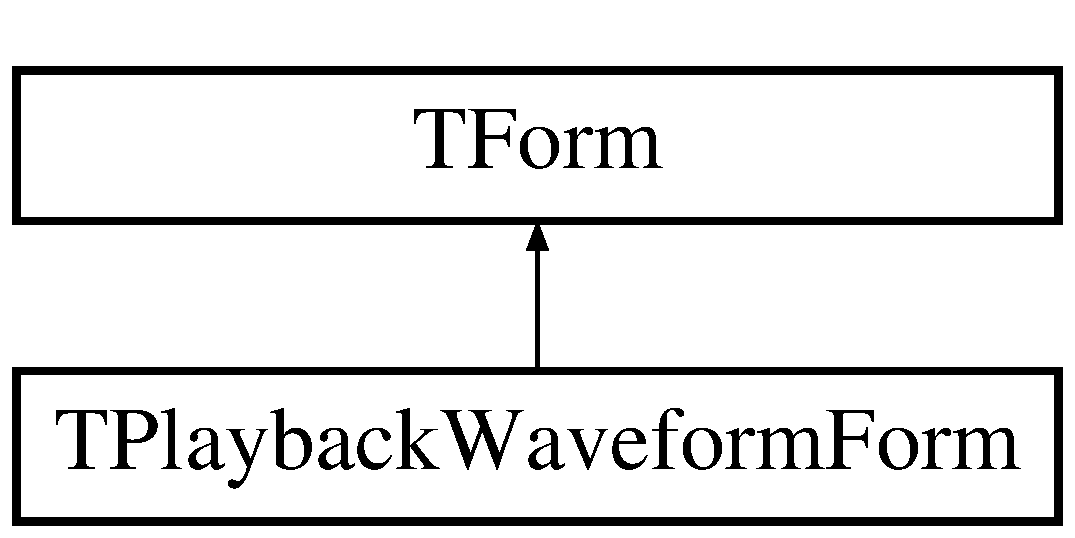
\includegraphics[height=2.000000cm]{class_t_playback_waveform_form}
\end{center}
\end{figure}
\subsection*{Public Member Functions}
\begin{DoxyCompactItemize}
\item 
\hypertarget{class_t_playback_waveform_form_a8cc695f219b19d6820bfd6f3f5273647}{void \+\_\+\+\_\+fastcall {\bfseries Browse\+Bit\+Btn\+Click} (T\+Object $\ast$Sender)}\label{class_t_playback_waveform_form_a8cc695f219b19d6820bfd6f3f5273647}

\item 
\hypertarget{class_t_playback_waveform_form_a86a4a88da3dcabc0207dce64f3a14b02}{void \+\_\+\+\_\+fastcall {\bfseries Channel\+Combo\+Box\+Change} (T\+Object $\ast$Sender)}\label{class_t_playback_waveform_form_a86a4a88da3dcabc0207dce64f3a14b02}

\item 
\hypertarget{class_t_playback_waveform_form_a4d6d83cafdeaa4319357e947edab4f7d}{void \+\_\+\+\_\+fastcall {\bfseries Convert\+Gain\+Edit\+Key\+Press} (T\+Object $\ast$Sender, wchar\+\_\+t \&Key)}\label{class_t_playback_waveform_form_a4d6d83cafdeaa4319357e947edab4f7d}

\item 
\hypertarget{class_t_playback_waveform_form_a393109c61194397fe8c4f955637b705c}{void \+\_\+\+\_\+fastcall {\bfseries Offset\+Edit\+Key\+Press} (T\+Object $\ast$Sender, wchar\+\_\+t \&Key)}\label{class_t_playback_waveform_form_a393109c61194397fe8c4f955637b705c}

\item 
\hypertarget{class_t_playback_waveform_form_a4e263a16a577705ae4458167542e3a01}{void \+\_\+\+\_\+fastcall {\bfseries Repeats\+Radio\+Group\+Click} (T\+Object $\ast$Sender)}\label{class_t_playback_waveform_form_a4e263a16a577705ae4458167542e3a01}

\item 
\hypertarget{class_t_playback_waveform_form_acab256b87f2d9dbd899f0bf671930230}{void \+\_\+\+\_\+fastcall {\bfseries Waveform\+Duration\+Edit\+Key\+Press} (T\+Object $\ast$Sender, wchar\+\_\+t \&Key)}\label{class_t_playback_waveform_form_acab256b87f2d9dbd899f0bf671930230}

\item 
\hypertarget{class_t_playback_waveform_form_a83b1e844dc4c1fc5bdbfb5c39be1bda2}{void \+\_\+\+\_\+fastcall {\bfseries Concatenate\+Episodes\+Check\+Box\+Click} (T\+Object $\ast$Sender)}\label{class_t_playback_waveform_form_a83b1e844dc4c1fc5bdbfb5c39be1bda2}

\item 
\hypertarget{class_t_playback_waveform_form_ab52ac2a55e0c2b60139a5468501247bd}{\+\_\+\+\_\+fastcall {\bfseries T\+Playback\+Waveform\+Form} (T\+Component $\ast$Owner)}\label{class_t_playback_waveform_form_ab52ac2a55e0c2b60139a5468501247bd}

\end{DoxyCompactItemize}
\subsection*{Public Attributes}
\begin{DoxyCompactItemize}
\item 
\hypertarget{class_t_playback_waveform_form_afda2f3c92c8fb1a49dc54f05cd6bf491}{T\+Open\+Dialog $\ast$ {\bfseries Open\+Dialog1}}\label{class_t_playback_waveform_form_afda2f3c92c8fb1a49dc54f05cd6bf491}

\item 
\hypertarget{class_t_playback_waveform_form_a00e31a3b56b6976cf204f3df4c1aa7c3}{T\+Image\+List $\ast$ {\bfseries Image\+List1}}\label{class_t_playback_waveform_form_a00e31a3b56b6976cf204f3df4c1aa7c3}

\item 
\hypertarget{class_t_playback_waveform_form_a8e6bb83d6cfc75b299bc4f10228ffa05}{T\+Label $\ast$ {\bfseries Label1}}\label{class_t_playback_waveform_form_a8e6bb83d6cfc75b299bc4f10228ffa05}

\item 
\hypertarget{class_t_playback_waveform_form_abec9e5d15d47b9fc3c270871d97f528f}{T\+Label $\ast$ {\bfseries File\+Label}}\label{class_t_playback_waveform_form_abec9e5d15d47b9fc3c270871d97f528f}

\item 
\hypertarget{class_t_playback_waveform_form_a8c695018a4294ec2806db3f09cc96837}{T\+Bit\+Btn $\ast$ {\bfseries Browse\+Bit\+Btn}}\label{class_t_playback_waveform_form_a8c695018a4294ec2806db3f09cc96837}

\item 
\hypertarget{class_t_playback_waveform_form_ab90a318d39d002159b327e9db4457a45}{T\+Label $\ast$ {\bfseries Label2}}\label{class_t_playback_waveform_form_ab90a318d39d002159b327e9db4457a45}

\item 
\hypertarget{class_t_playback_waveform_form_a27c2ed75f913ebcd0862c6b6aa6ca3ba}{T\+Combo\+Box $\ast$ {\bfseries Channel\+Combo\+Box}}\label{class_t_playback_waveform_form_a27c2ed75f913ebcd0862c6b6aa6ca3ba}

\item 
\hypertarget{class_t_playback_waveform_form_ab2bce771ff73c1555cc36007c904c838}{T\+Radio\+Group $\ast$ {\bfseries Repeats\+Radio\+Group}}\label{class_t_playback_waveform_form_ab2bce771ff73c1555cc36007c904c838}

\item 
\hypertarget{class_t_playback_waveform_form_a03f5d62cf9aa5bf2f165e24305bd945d}{T\+Label $\ast$ {\bfseries Label8}}\label{class_t_playback_waveform_form_a03f5d62cf9aa5bf2f165e24305bd945d}

\item 
\hypertarget{class_t_playback_waveform_form_ae36df9fa89e9305db983061981f6db9f}{T\+Edit $\ast$ {\bfseries Fixed\+Repeats\+Edit}}\label{class_t_playback_waveform_form_ae36df9fa89e9305db983061981f6db9f}

\item 
\hypertarget{class_t_playback_waveform_form_ad0f261df3ef789442dc8e0dc8a94570f}{T\+Group\+Box $\ast$ {\bfseries Group\+Box1}}\label{class_t_playback_waveform_form_ad0f261df3ef789442dc8e0dc8a94570f}

\item 
\hypertarget{class_t_playback_waveform_form_a765616f2a40752567f3eb2871daa31a3}{T\+Label $\ast$ {\bfseries Conversion\+Label}}\label{class_t_playback_waveform_form_a765616f2a40752567f3eb2871daa31a3}

\item 
\hypertarget{class_t_playback_waveform_form_ad7f3155b99ae07b1c885a245d806fa9f}{T\+Label $\ast$ {\bfseries Label5}}\label{class_t_playback_waveform_form_ad7f3155b99ae07b1c885a245d806fa9f}

\item 
\hypertarget{class_t_playback_waveform_form_a5da72b0337f94b39ac77ef8c47c70eda}{T\+Edit $\ast$ {\bfseries Convert\+Gain\+Edit}}\label{class_t_playback_waveform_form_a5da72b0337f94b39ac77ef8c47c70eda}

\item 
\hypertarget{class_t_playback_waveform_form_af093a55e2645f0cf491aad721aa55988}{T\+Label $\ast$ {\bfseries Label6}}\label{class_t_playback_waveform_form_af093a55e2645f0cf491aad721aa55988}

\item 
\hypertarget{class_t_playback_waveform_form_aab0a9b2f139ef9cdb76caaaf99f69445}{T\+Edit $\ast$ {\bfseries Offset\+Edit}}\label{class_t_playback_waveform_form_aab0a9b2f139ef9cdb76caaaf99f69445}

\item 
\hypertarget{class_t_playback_waveform_form_a7c146a7e954fbde6c06c52427a9cfb23}{T\+Group\+Box $\ast$ {\bfseries Sampling\+Settings\+Group\+Box}}\label{class_t_playback_waveform_form_a7c146a7e954fbde6c06c52427a9cfb23}

\item 
\hypertarget{class_t_playback_waveform_form_a7952d55a3874f58fff481a97a06f2134}{T\+Edit $\ast$ {\bfseries Waveform\+Duration\+Edit}}\label{class_t_playback_waveform_form_a7952d55a3874f58fff481a97a06f2134}

\item 
\hypertarget{class_t_playback_waveform_form_a004cf0eb7719720ffb53493904a471c8}{T\+Label $\ast$ {\bfseries Waveform\+Duration\+Label}}\label{class_t_playback_waveform_form_a004cf0eb7719720ffb53493904a471c8}

\item 
\hypertarget{class_t_playback_waveform_form_a70aa53949c81bb695c00b78d82f271cf}{T\+Label $\ast$ {\bfseries Label3}}\label{class_t_playback_waveform_form_a70aa53949c81bb695c00b78d82f271cf}

\item 
\hypertarget{class_t_playback_waveform_form_a665920f138dbcbe1f842ecd9b7b6f348}{T\+Label $\ast$ {\bfseries Label4}}\label{class_t_playback_waveform_form_a665920f138dbcbe1f842ecd9b7b6f348}

\item 
\hypertarget{class_t_playback_waveform_form_a69a8cccb70f515d64b8a657a8fac8a24}{T\+P\+L\+O\+T\+Panel $\ast$ {\bfseries Plot\+Panel1}}\label{class_t_playback_waveform_form_a69a8cccb70f515d64b8a657a8fac8a24}

\item 
\hypertarget{class_t_playback_waveform_form_ac6996da2d933f13bc18a967effc3fc83}{T\+Check\+Box $\ast$ {\bfseries Concatenate\+Episodes\+Check\+Box}}\label{class_t_playback_waveform_form_ac6996da2d933f13bc18a967effc3fc83}

\item 
\hypertarget{class_t_playback_waveform_form_a6960a95e9c3e7017cec01956274992b3}{T\+Edit $\ast$ {\bfseries Delay\+Between\+Repeats\+Edit}}\label{class_t_playback_waveform_form_a6960a95e9c3e7017cec01956274992b3}

\item 
\hypertarget{class_t_playback_waveform_form_a1b338144973085568e7769b6a5d39b5d}{T\+Label $\ast$ {\bfseries Label7}}\label{class_t_playback_waveform_form_a1b338144973085568e7769b6a5d39b5d}

\item 
\hypertarget{class_t_playback_waveform_form_a697591f3fee286e078c63d5fbbfb50d7}{\hyperlink{class_t_playback_waveform}{T\+Playback\+Waveform} $\ast$ {\bfseries Waveform}}\label{class_t_playback_waveform_form_a697591f3fee286e078c63d5fbbfb50d7}

\end{DoxyCompactItemize}


\subsection{Detailed Description}
G\+U\+I Editor for \hyperlink{class_t_playback_waveform}{T\+Playback\+Waveform}. 

\begin{DoxyAuthor}{Author}
E. Brady Trexler $<$ebtrexler (at) gothamsci.\+com$>$, 2011 -\/ 2013 
\end{DoxyAuthor}


The documentation for this class was generated from the following files\+:\begin{DoxyCompactItemize}
\item 
G\+U\+I\+\_\+\+Playback\+Waveform\+Form.\+h\item 
G\+U\+I\+\_\+\+Playback\+Waveform\+Form.\+cpp\end{DoxyCompactItemize}

\hypertarget{struct_t_rational_fraction}{\section{T\+Rational\+Fraction Struct Reference}
\label{struct_t_rational_fraction}\index{T\+Rational\+Fraction@{T\+Rational\+Fraction}}
}


Used by R\+A\+R\+N -\/rational approximation to given real number.  




{\ttfamily \#include $<$R\+A\+R\+N.\+h$>$}

\subsection*{Public Attributes}
\begin{DoxyCompactItemize}
\item 
\hypertarget{struct_t_rational_fraction_a786ee34180c2c499b366dd96012dce59}{int {\bfseries Numerator}}\label{struct_t_rational_fraction_a786ee34180c2c499b366dd96012dce59}

\item 
\hypertarget{struct_t_rational_fraction_aa4a827775f6547a4e6c40e4b4eb663f3}{int {\bfseries Denominator}}\label{struct_t_rational_fraction_aa4a827775f6547a4e6c40e4b4eb663f3}

\end{DoxyCompactItemize}


\subsection{Detailed Description}
Used by R\+A\+R\+N -\/rational approximation to given real number. 

The documentation for this struct was generated from the following file\+:\begin{DoxyCompactItemize}
\item 
R\+A\+R\+N.\+h\end{DoxyCompactItemize}

\hypertarget{class_t_r_t_base}{\section{T\+R\+T\+Base Class Reference}
\label{class_t_r_t_base}\index{T\+R\+T\+Base@{T\+R\+T\+Base}}
}


Base class for all derived classes used in the network.  




{\ttfamily \#include $<$R\+T\+\_\+\+Base.\+h$>$}

Inheritance diagram for T\+R\+T\+Base\+:\begin{figure}[H]
\begin{center}
\leavevmode
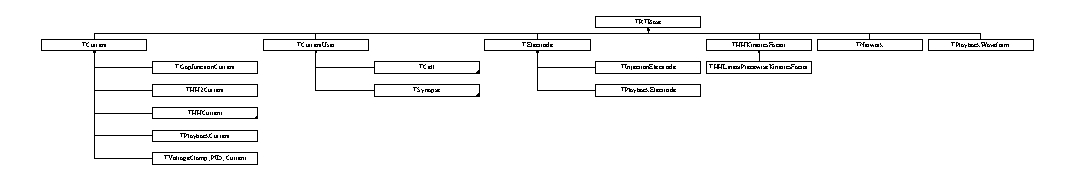
\includegraphics[height=1.988838cm]{class_t_r_t_base}
\end{center}
\end{figure}
\subsection*{Public Member Functions}
\begin{DoxyCompactItemize}
\item 
\hypertarget{class_t_r_t_base_a1c20ffac4117eccf2011d2a93147cef7}{const std\+::wstring \+\_\+\+\_\+fastcall \hyperlink{class_t_r_t_base_a1c20ffac4117eccf2011d2a93147cef7}{Class\+Type} () const }\label{class_t_r_t_base_a1c20ffac4117eccf2011d2a93147cef7}

\begin{DoxyCompactList}\small\item\em Returns R\+T\+T\+I on class type. \end{DoxyCompactList}\item 
virtual const std\+::wstring \\*
\&\+\_\+\+\_\+fastcall \hyperlink{class_t_r_t_base_a6083fd510cbcb00faa85e5934fc3c18e}{Class\+Key} () const =0
\begin{DoxyCompactList}\small\item\em Returns string used to register class with factory. \end{DoxyCompactList}\item 
\hypertarget{class_t_r_t_base_a2da78a149d3253738c69e2b180975819}{const std\+::wstring \+\_\+\+\_\+fastcall \hyperlink{class_t_r_t_base_a2da78a149d3253738c69e2b180975819}{Name} () const }\label{class_t_r_t_base_a2da78a149d3253738c69e2b180975819}

\begin{DoxyCompactList}\small\item\em Returns name of object (should be unique in network) \end{DoxyCompactList}\item 
\hypertarget{class_t_r_t_base_ac067ba851b9fe12a4a8d5f8305dd0333}{void \+\_\+\+\_\+fastcall \hyperlink{class_t_r_t_base_ac067ba851b9fe12a4a8d5f8305dd0333}{Set\+Name} (const std\+::wstring \&name)}\label{class_t_r_t_base_ac067ba851b9fe12a4a8d5f8305dd0333}

\begin{DoxyCompactList}\small\item\em User supplied name of object -- must be unique in network. \end{DoxyCompactList}\item 
\hypertarget{class_t_r_t_base_a6134ae5c10efab0cbdc42b20930495b1}{const bool \+\_\+\+\_\+fastcall \hyperlink{class_t_r_t_base_a6134ae5c10efab0cbdc42b20930495b1}{Is\+Active} () const }\label{class_t_r_t_base_a6134ae5c10efab0cbdc42b20930495b1}

\begin{DoxyCompactList}\small\item\em Determines if object is included in model. \end{DoxyCompactList}\item 
\hypertarget{class_t_r_t_base_a80f01fe30e7b4c979dd420bb3f41aef0}{void \+\_\+\+\_\+fastcall \hyperlink{class_t_r_t_base_a80f01fe30e7b4c979dd420bb3f41aef0}{Set\+Active} (bool active)}\label{class_t_r_t_base_a80f01fe30e7b4c979dd420bb3f41aef0}

\begin{DoxyCompactList}\small\item\em Determines if object is included in model. \end{DoxyCompactList}\item 
\hypertarget{class_t_r_t_base_a06f28e5bca2187b9ebcea8c2bc367f98}{const int \+\_\+\+\_\+fastcall \hyperlink{class_t_r_t_base_a06f28e5bca2187b9ebcea8c2bc367f98}{Get\+X} () const }\label{class_t_r_t_base_a06f28e5bca2187b9ebcea8c2bc367f98}

\begin{DoxyCompactList}\small\item\em Position of item on G\+U\+I representation of network. \end{DoxyCompactList}\item 
\hypertarget{class_t_r_t_base_ac727c29c5b1fbad3bd45efdb03f1b5f0}{void \+\_\+\+\_\+fastcall \hyperlink{class_t_r_t_base_ac727c29c5b1fbad3bd45efdb03f1b5f0}{Set\+X} (int x)}\label{class_t_r_t_base_ac727c29c5b1fbad3bd45efdb03f1b5f0}

\begin{DoxyCompactList}\small\item\em Position of item on G\+U\+I representation of network. \end{DoxyCompactList}\item 
\hypertarget{class_t_r_t_base_aa06da8b3fa1116a2e12f64fb3f408dde}{const int \+\_\+\+\_\+fastcall \hyperlink{class_t_r_t_base_aa06da8b3fa1116a2e12f64fb3f408dde}{Get\+Y} () const }\label{class_t_r_t_base_aa06da8b3fa1116a2e12f64fb3f408dde}

\begin{DoxyCompactList}\small\item\em Position of item on G\+U\+I representation of network. \end{DoxyCompactList}\item 
\hypertarget{class_t_r_t_base_af874732b636ea9a9ce26fb393e283b51}{void \+\_\+\+\_\+fastcall \hyperlink{class_t_r_t_base_af874732b636ea9a9ce26fb393e283b51}{Set\+Y} (int y)}\label{class_t_r_t_base_af874732b636ea9a9ce26fb393e283b51}

\begin{DoxyCompactList}\small\item\em Position of item on G\+U\+I representation of network. \end{DoxyCompactList}\item 
\hypertarget{class_t_r_t_base_a197af02c2de02e8320dd659474a4e74b}{bool \+\_\+\+\_\+fastcall \hyperlink{class_t_r_t_base_a197af02c2de02e8320dd659474a4e74b}{Hit\+Test} (int X, int Y, int tol=0) const }\label{class_t_r_t_base_a197af02c2de02e8320dd659474a4e74b}

\begin{DoxyCompactList}\small\item\em For use with G\+U\+I -- tests X and Y for proximity to stored values. \end{DoxyCompactList}\item 
const bool \+\_\+\+\_\+fastcall \hyperlink{class_t_r_t_base_acd50b266b33d3db3142f4ef0b0e8a7d8}{Attach\+Edit\+Form\+To} (T\+Component $\ast$Owner, T\+Win\+Control $\ast$Parent)
\begin{DoxyCompactList}\small\item\em G\+U\+I method -- G\+U\+I calls this to get the V\+C\+L form to show in the G\+U\+I. \end{DoxyCompactList}\item 
\hypertarget{class_t_r_t_base_a42793e9cca7c36b284457c8483f1718b}{virtual void \+\_\+\+\_\+fastcall \hyperlink{class_t_r_t_base_a42793e9cca7c36b284457c8483f1718b}{Populate\+Edit\+Form} ()=0}\label{class_t_r_t_base_a42793e9cca7c36b284457c8483f1718b}

\begin{DoxyCompactList}\small\item\em Interface for derived classes, called by G\+U\+I to update V\+C\+L form components. \end{DoxyCompactList}\item 
\hypertarget{class_t_r_t_base_aa00f2ee3d1c785f8a46ca16deef674c7}{virtual bool \+\_\+\+\_\+fastcall \hyperlink{class_t_r_t_base_aa00f2ee3d1c785f8a46ca16deef674c7}{Validate\+Edit\+Form} ()=0}\label{class_t_r_t_base_aa00f2ee3d1c785f8a46ca16deef674c7}

\begin{DoxyCompactList}\small\item\em Interface for derived classes, called by G\+U\+I to read V\+C\+L form values. \end{DoxyCompactList}\item 
\hypertarget{class_t_r_t_base_a50d3183e5a738cfbb5bbd8b0cb7c5f89}{virtual bool \+\_\+\+\_\+fastcall \hyperlink{class_t_r_t_base_a50d3183e5a738cfbb5bbd8b0cb7c5f89}{Initialize} (bool Reset)=0}\label{class_t_r_t_base_a50d3183e5a738cfbb5bbd8b0cb7c5f89}

\begin{DoxyCompactList}\small\item\em pure virtual function for resetting before networking run \end{DoxyCompactList}\item 
virtual void $\ast$const \+\_\+\+\_\+fastcall \hyperlink{class_t_r_t_base_ab83e520005e20ee71f98f3e85e1ee6d4}{Get\+Edit\+Form} ()=0
\item 
\hypertarget{class_t_r_t_base_a5d257475501e327079c06858de645854}{\+\_\+\+\_\+fastcall \hyperlink{class_t_r_t_base_a5d257475501e327079c06858de645854}{T\+R\+T\+Base} ()}\label{class_t_r_t_base_a5d257475501e327079c06858de645854}

\begin{DoxyCompactList}\small\item\em Default constructor. \end{DoxyCompactList}\item 
\hypertarget{class_t_r_t_base_ac1b2d91a880b9cf6d951980c85b6d672}{\+\_\+\+\_\+fastcall \hyperlink{class_t_r_t_base_ac1b2d91a880b9cf6d951980c85b6d672}{T\+R\+T\+Base} (const std\+::wstring \&name, const bool active=true)}\label{class_t_r_t_base_ac1b2d91a880b9cf6d951980c85b6d672}

\begin{DoxyCompactList}\small\item\em Specialized constructor. \end{DoxyCompactList}\item 
\hypertarget{class_t_r_t_base_a2f4e179ec98c38249da18d437965a4a7}{\+\_\+\+\_\+fastcall \hyperlink{class_t_r_t_base_a2f4e179ec98c38249da18d437965a4a7}{T\+R\+T\+Base} (const \hyperlink{class_t_r_t_base}{T\+R\+T\+Base} \&source)}\label{class_t_r_t_base_a2f4e179ec98c38249da18d437965a4a7}

\begin{DoxyCompactList}\small\item\em Copy constructor. \end{DoxyCompactList}\item 
\hypertarget{class_t_r_t_base_aef9192c65718aedd3bbd90ddb397b364}{\hyperlink{class_t_r_t_base}{T\+R\+T\+Base} \& \hyperlink{class_t_r_t_base_aef9192c65718aedd3bbd90ddb397b364}{operator=} (const \hyperlink{class_t_r_t_base}{T\+R\+T\+Base} \&source)}\label{class_t_r_t_base_aef9192c65718aedd3bbd90ddb397b364}

\begin{DoxyCompactList}\small\item\em Overloaded assignment operator. \end{DoxyCompactList}\end{DoxyCompactItemize}
\subsection*{Protected Member Functions}
\begin{DoxyCompactItemize}
\item 
\hypertarget{class_t_r_t_base_a5db5960db25eecaf9df5b09463da59eb}{virtual void const \+\_\+\+\_\+fastcall \hyperlink{class_t_r_t_base_a5db5960db25eecaf9df5b09463da59eb}{Write\+To\+Stream} (ostream \&stream) const =0}\label{class_t_r_t_base_a5db5960db25eecaf9df5b09463da59eb}

\begin{DoxyCompactList}\small\item\em pure virtual function for derived classes to write to a stream \end{DoxyCompactList}\item 
\hypertarget{class_t_r_t_base_af68d8bc77ec5893fea6ca486cdd136fc}{virtual void const \+\_\+\+\_\+fastcall \hyperlink{class_t_r_t_base_af68d8bc77ec5893fea6ca486cdd136fc}{Read\+From\+Stream} (istream \&stream)=0}\label{class_t_r_t_base_af68d8bc77ec5893fea6ca486cdd136fc}

\begin{DoxyCompactList}\small\item\em pure virtual function for derived classes to read from a stream \end{DoxyCompactList}\end{DoxyCompactItemize}
\subsection*{Friends}
\begin{DoxyCompactItemize}
\item 
\hypertarget{class_t_r_t_base_ac98d07dd8f7b70e16ccb9a01abf56b9c}{class \hyperlink{class_t_r_t_base_ac98d07dd8f7b70e16ccb9a01abf56b9c}{boost\+::serialization\+::access}}\label{class_t_r_t_base_ac98d07dd8f7b70e16ccb9a01abf56b9c}

\begin{DoxyCompactList}\small\item\em Required for serialization and saving networks to disk. \end{DoxyCompactList}\item 
\hypertarget{class_t_r_t_base_a64356ce8469c8ed650b40c9e8ad51c27}{ostream \& \hyperlink{class_t_r_t_base_a64356ce8469c8ed650b40c9e8ad51c27}{operator$<$$<$} (ostream \&stream, const \hyperlink{class_t_r_t_base}{T\+R\+T\+Base} \&rtbase)}\label{class_t_r_t_base_a64356ce8469c8ed650b40c9e8ad51c27}

\begin{DoxyCompactList}\small\item\em insertion $<$$<$ operator that calls pure virtual method Write\+To\+Stream \end{DoxyCompactList}\item 
\hypertarget{class_t_r_t_base_afb059842172db7fea14d8d5f360d83b7}{istream \& \hyperlink{class_t_r_t_base_afb059842172db7fea14d8d5f360d83b7}{operator$>$$>$} (istream \&stream, \hyperlink{class_t_r_t_base}{T\+R\+T\+Base} \&rtbase)}\label{class_t_r_t_base_afb059842172db7fea14d8d5f360d83b7}

\begin{DoxyCompactList}\small\item\em extraction $>$$>$ operator that calls pure virtual method Read\+From\+Stream \end{DoxyCompactList}\end{DoxyCompactItemize}


\subsection{Detailed Description}
Base class for all derived classes used in the network. 

\begin{DoxyAuthor}{Author}
E. Brady Trexler $<$ebtrexler (at) gothamsci.\+com$>$, 2011 -\/ 2013 
\end{DoxyAuthor}


\subsection{Member Function Documentation}
\hypertarget{class_t_r_t_base_acd50b266b33d3db3142f4ef0b0e8a7d8}{\index{T\+R\+T\+Base@{T\+R\+T\+Base}!Attach\+Edit\+Form\+To@{Attach\+Edit\+Form\+To}}
\index{Attach\+Edit\+Form\+To@{Attach\+Edit\+Form\+To}!T\+R\+T\+Base@{T\+R\+T\+Base}}
\subsubsection[{Attach\+Edit\+Form\+To}]{\setlength{\rightskip}{0pt plus 5cm}const bool \+\_\+\+\_\+fastcall T\+R\+T\+Base\+::\+Attach\+Edit\+Form\+To (
\begin{DoxyParamCaption}
\item[{T\+Component $\ast$}]{Owner, }
\item[{T\+Win\+Control $\ast$}]{Parent}
\end{DoxyParamCaption}
)}}\label{class_t_r_t_base_acd50b266b33d3db3142f4ef0b0e8a7d8}


G\+U\+I method -- G\+U\+I calls this to get the V\+C\+L form to show in the G\+U\+I. 

This is the only platform dependent method in the network class framework. Other implementations should alter this function to match G\+U\+I requirements. \hypertarget{class_t_r_t_base_a6083fd510cbcb00faa85e5934fc3c18e}{\index{T\+R\+T\+Base@{T\+R\+T\+Base}!Class\+Key@{Class\+Key}}
\index{Class\+Key@{Class\+Key}!T\+R\+T\+Base@{T\+R\+T\+Base}}
\subsubsection[{Class\+Key}]{\setlength{\rightskip}{0pt plus 5cm}virtual const std\+::wstring\& \+\_\+\+\_\+fastcall T\+R\+T\+Base\+::\+Class\+Key (
\begin{DoxyParamCaption}
{}
\end{DoxyParamCaption}
) const\hspace{0.3cm}{\ttfamily [pure virtual]}}}\label{class_t_r_t_base_a6083fd510cbcb00faa85e5934fc3c18e}


Returns string used to register class with factory. 

Users of class factories must also tell the class the key they used when registering the class. See factory.\+h 

Implemented in \hyperlink{class_t_network_a9af68c6c12402bf185c1de44bab29a17}{T\+Network}, \hyperlink{class_t_h_h2_current_aede58e5114cd7b8284430badd4c29f3e}{T\+H\+H2\+Current}, \hyperlink{class_t_playback_waveform_ad5bb30fcf319f49b1119881d857262fa}{T\+Playback\+Waveform}, \hyperlink{class_t_h_h_linear_piecewise_current_a2f62f65488ad9489bdf671b6fd4dd837}{T\+H\+H\+Linear\+Piecewise\+Current}, \hyperlink{class_t_biological_cell_a7006d17ad9b7cdfa4b637d32a3c6b0b5}{T\+Biological\+Cell}, \hyperlink{class_t_playback_current_aabc05c6ace3f33105e3c0645785cc38a}{T\+Playback\+Current}, \hyperlink{class_t_h_h_kinetics_factor_ac161d432e14597146b0bd45cbed7e225}{T\+H\+H\+Kinetics\+Factor}, \hyperlink{class_t_playback_cell_a8e35ecdb1be99d97349d8904b6064e5d}{T\+Playback\+Cell}, \hyperlink{class_t_h_h_linear_piecewise_kinetics_factor_a2129c509478fcca9cb2479817856c0bf}{T\+H\+H\+Linear\+Piecewise\+Kinetics\+Factor}, \hyperlink{class_t_voltage_clamp___p_i_d___current_a7be7d4e60396298cad6617d0ab6cfd34}{T\+Voltage\+Clamp\+\_\+\+P\+I\+D\+\_\+\+Current}, \hyperlink{class_t_playback_electrode_ab1174a8ccda8d316130a899471341374}{T\+Playback\+Electrode}, \hyperlink{class_t_model_cell_aaaffe113670920605dffda564b475ad0}{T\+Model\+Cell}, \hyperlink{class_t_injection_electrode_ad13dada3837856466fd9321afee58166}{T\+Injection\+Electrode}, \hyperlink{class_t_h_h_current_a49049acfa420622d26011f881c432329}{T\+H\+H\+Current}, \hyperlink{class_t_gap_junction_synapse_abe213c6289ba13e7ca700132fd3f9793}{T\+Gap\+Junction\+Synapse}, \hyperlink{class_t_gen_bi_dir_synapse_a7a704a5acb3ec4a36487a762fe87f784}{T\+Gen\+Bi\+Dir\+Synapse}, and \hyperlink{class_t_gap_junction_current_af3f5986036ba62eb9d4441e72ccff617}{T\+Gap\+Junction\+Current}.

\hypertarget{class_t_r_t_base_ab83e520005e20ee71f98f3e85e1ee6d4}{\index{T\+R\+T\+Base@{T\+R\+T\+Base}!Get\+Edit\+Form@{Get\+Edit\+Form}}
\index{Get\+Edit\+Form@{Get\+Edit\+Form}!T\+R\+T\+Base@{T\+R\+T\+Base}}
\subsubsection[{Get\+Edit\+Form}]{\setlength{\rightskip}{0pt plus 5cm}void $\ast$const \+\_\+\+\_\+fastcall T\+R\+T\+Base\+::\+Get\+Edit\+Form (
\begin{DoxyParamCaption}
{}
\end{DoxyParamCaption}
)\hspace{0.3cm}{\ttfamily [pure virtual]}}}\label{class_t_r_t_base_ab83e520005e20ee71f98f3e85e1ee6d4}
Interface for derived classes, returns pointer to G\+U\+I object for editing members. Callers must cast pointer to the correct object. 

Implemented in \hyperlink{class_t_h_h2_current_a8b78e8e4d6abfe5bac5a8ac256b4e093}{T\+H\+H2\+Current}, \hyperlink{class_t_playback_waveform_a1fcb2c8d237e2418080fdefeb3e13f73}{T\+Playback\+Waveform}, \hyperlink{class_t_injection_electrode_a825ef8d17c3e3612aeb6b53c9e3aa539}{T\+Injection\+Electrode}, \hyperlink{class_t_voltage_clamp___p_i_d___current_a065e523cb852fbca91bd13e5a93bf293}{T\+Voltage\+Clamp\+\_\+\+P\+I\+D\+\_\+\+Current}, \hyperlink{class_t_h_h_current_a3529515fbe5fbcce14fedca3a8db5e04}{T\+H\+H\+Current}, \hyperlink{class_t_h_h_linear_piecewise_current_a9a240a941e2a98fc5bebf3ffb255541c}{T\+H\+H\+Linear\+Piecewise\+Current}, \hyperlink{class_t_model_cell_af69daf6390baa3fc7ba7c11aa0d726ad}{T\+Model\+Cell}, \hyperlink{class_t_playback_current_a28d0a767401ce8b53de441e83c6aae5c}{T\+Playback\+Current}, \hyperlink{class_t_playback_electrode_af870739aeec24862ed6333dc453951a1}{T\+Playback\+Electrode}, \hyperlink{class_t_gap_junction_synapse_ad1bfccafcf7a340e61d76e9ffa340b63}{T\+Gap\+Junction\+Synapse}, \hyperlink{class_t_playback_cell_a5cd1500e6e80753779d7dee74f4b84d2}{T\+Playback\+Cell}, \hyperlink{class_t_biological_cell_a35a6350ccd6c518944f15902edc1c608}{T\+Biological\+Cell}, \hyperlink{class_t_gen_bi_dir_synapse_ada612e93b0d7a24ea55201e364bdf7cd}{T\+Gen\+Bi\+Dir\+Synapse}, and \hyperlink{class_t_gap_junction_current_a778ffd1b6c6d72562ad03fa42ef6b55f}{T\+Gap\+Junction\+Current}.



The documentation for this class was generated from the following files\+:\begin{DoxyCompactItemize}
\item 
R\+T\+\_\+\+Base.\+h\item 
R\+T\+\_\+\+Base.\+cpp\end{DoxyCompactItemize}

\hypertarget{class_t_run_dynamic_clamp_form}{\section{T\+Run\+Dynamic\+Clamp\+Form Class Reference}
\label{class_t_run_dynamic_clamp_form}\index{T\+Run\+Dynamic\+Clamp\+Form@{T\+Run\+Dynamic\+Clamp\+Form}}
}


Graphical interface for running simulation or dynamic clamp or hybrid.  




{\ttfamily \#include $<$G\+U\+I\+\_\+\+Run\+Model\+Form.\+h$>$}

Inheritance diagram for T\+Run\+Dynamic\+Clamp\+Form\+:\begin{figure}[H]
\begin{center}
\leavevmode
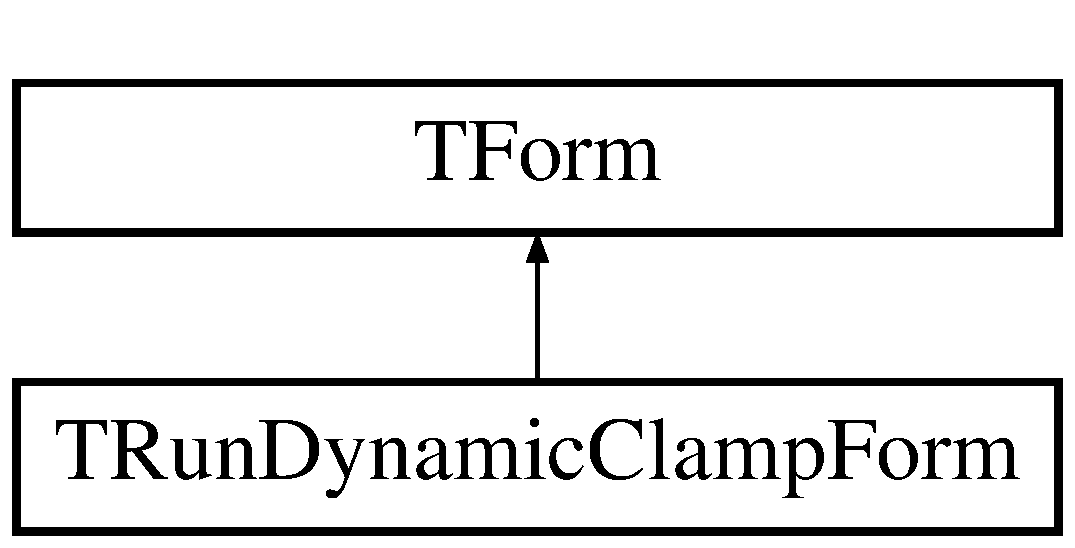
\includegraphics[height=2.000000cm]{class_t_run_dynamic_clamp_form}
\end{center}
\end{figure}
\subsection*{Public Member Functions}
\begin{DoxyCompactItemize}
\item 
\hypertarget{class_t_run_dynamic_clamp_form_ab03c9033d9ecb26a60c5bf00e1faa5a8}{void \+\_\+\+\_\+fastcall {\bfseries Start\+Action\+Update} (T\+Object $\ast$Sender)}\label{class_t_run_dynamic_clamp_form_ab03c9033d9ecb26a60c5bf00e1faa5a8}

\item 
\hypertarget{class_t_run_dynamic_clamp_form_a45d05f75d4f7cb5e5684bcd9b1619986}{void \+\_\+\+\_\+fastcall {\bfseries Stop\+Action\+Update} (T\+Object $\ast$Sender)}\label{class_t_run_dynamic_clamp_form_a45d05f75d4f7cb5e5684bcd9b1619986}

\item 
\hypertarget{class_t_run_dynamic_clamp_form_a24e6032e5c7e32d7762a48cd4da639d6}{void \+\_\+\+\_\+fastcall {\bfseries Start\+Action\+Execute} (T\+Object $\ast$Sender)}\label{class_t_run_dynamic_clamp_form_a24e6032e5c7e32d7762a48cd4da639d6}

\item 
\hypertarget{class_t_run_dynamic_clamp_form_aa7e994758a90e6976dcefb43e08784b0}{void \+\_\+\+\_\+fastcall {\bfseries Stop\+Action\+Execute} (T\+Object $\ast$Sender)}\label{class_t_run_dynamic_clamp_form_aa7e994758a90e6976dcefb43e08784b0}

\item 
\hypertarget{class_t_run_dynamic_clamp_form_af3bfbdfeef75cf56f436a80e6083447c}{void \+\_\+\+\_\+fastcall {\bfseries Close\+Action\+Execute} (T\+Object $\ast$Sender)}\label{class_t_run_dynamic_clamp_form_af3bfbdfeef75cf56f436a80e6083447c}

\item 
\hypertarget{class_t_run_dynamic_clamp_form_a9a8a602e10f6bb9f3928cc6040f12af6}{void \+\_\+\+\_\+fastcall {\bfseries Add\+To\+Display\+Button\+Click} (T\+Object $\ast$Sender)}\label{class_t_run_dynamic_clamp_form_a9a8a602e10f6bb9f3928cc6040f12af6}

\item 
\hypertarget{class_t_run_dynamic_clamp_form_a7a14bf15b3d83463473d5a2690ea32b5}{void \+\_\+\+\_\+fastcall {\bfseries Remove\+From\+Display\+Button\+Click} (T\+Object $\ast$Sender)}\label{class_t_run_dynamic_clamp_form_a7a14bf15b3d83463473d5a2690ea32b5}

\item 
\hypertarget{class_t_run_dynamic_clamp_form_a57849d37edd05724646f2a19a6b5b3e9}{void \+\_\+\+\_\+fastcall {\bfseries Clear\+Display\+List\+Button\+Click} (T\+Object $\ast$Sender)}\label{class_t_run_dynamic_clamp_form_a57849d37edd05724646f2a19a6b5b3e9}

\item 
\hypertarget{class_t_run_dynamic_clamp_form_a160d7ba495f32a232af213dc4f9529dc}{void \+\_\+\+\_\+fastcall {\bfseries C\+G\+M\+\_\+\+Button\+Click} (T\+Object $\ast$Sender)}\label{class_t_run_dynamic_clamp_form_a160d7ba495f32a232af213dc4f9529dc}

\item 
\hypertarget{class_t_run_dynamic_clamp_form_a031c331ed9e2f306abd8ca15529286a4}{void \+\_\+\+\_\+fastcall {\bfseries Save\+Data\+Check\+Box\+Click} (T\+Object $\ast$Sender)}\label{class_t_run_dynamic_clamp_form_a031c331ed9e2f306abd8ca15529286a4}

\item 
\hypertarget{class_t_run_dynamic_clamp_form_ac4e5f6ce8d2e491db75be6204af0d748}{void \+\_\+\+\_\+fastcall {\bfseries File\+Params\+Button\+Click} (T\+Object $\ast$Sender)}\label{class_t_run_dynamic_clamp_form_ac4e5f6ce8d2e491db75be6204af0d748}

\item 
\hypertarget{class_t_run_dynamic_clamp_form_af79c8113af87b17f48a9393bf0aca294}{void \+\_\+\+\_\+fastcall {\bfseries Form\+Close} (T\+Object $\ast$Sender, T\+Close\+Action \&Action)}\label{class_t_run_dynamic_clamp_form_af79c8113af87b17f48a9393bf0aca294}

\item 
\hypertarget{class_t_run_dynamic_clamp_form_a2de7e6942e073d984b80dab1f8dd48e5}{void \+\_\+\+\_\+fastcall {\bfseries Edit\+Key\+Press} (T\+Object $\ast$Sender, wchar\+\_\+t \&Key)}\label{class_t_run_dynamic_clamp_form_a2de7e6942e073d984b80dab1f8dd48e5}

\item 
\hypertarget{class_t_run_dynamic_clamp_form_a68cf1efe77c3e8f061370e64b0b6fa83}{void \+\_\+\+\_\+fastcall {\bfseries Data\+Logging\+List\+Box\+Click} (T\+Object $\ast$Sender)}\label{class_t_run_dynamic_clamp_form_a68cf1efe77c3e8f061370e64b0b6fa83}

\item 
\hypertarget{class_t_run_dynamic_clamp_form_ae24c6e2572703ad0624868566f3ede2e}{void \+\_\+\+\_\+fastcall {\bfseries Interpolate\+Check\+Box\+Click} (T\+Object $\ast$Sender)}\label{class_t_run_dynamic_clamp_form_ae24c6e2572703ad0624868566f3ede2e}

\item 
\hypertarget{class_t_run_dynamic_clamp_form_a5226faef0e5d4d407c910deb14e12142}{void \+\_\+\+\_\+fastcall {\bfseries Interpolate\+Rate\+Edit\+Key\+Press} (T\+Object $\ast$Sender, wchar\+\_\+t \&Key)}\label{class_t_run_dynamic_clamp_form_a5226faef0e5d4d407c910deb14e12142}

\item 
\hypertarget{class_t_run_dynamic_clamp_form_a804dee7362b2d4d065934aca9da2e841}{void \+\_\+\+\_\+fastcall {\bfseries Log\+Kinetic\+Params\+Button\+Click} (T\+Object $\ast$Sender)}\label{class_t_run_dynamic_clamp_form_a804dee7362b2d4d065934aca9da2e841}

\item 
\hypertarget{class_t_run_dynamic_clamp_form_afbb21fc67bfdeb495e64dca3a361fdbb}{void \+\_\+\+\_\+fastcall {\bfseries Log\+Kinetic\+Params\+Check\+Box\+Click} (T\+Object $\ast$Sender)}\label{class_t_run_dynamic_clamp_form_afbb21fc67bfdeb495e64dca3a361fdbb}

\item 
\hypertarget{class_t_run_dynamic_clamp_form_a2a0e14a44c7c74c29b1d9db72f939aa6}{void \+\_\+\+\_\+fastcall {\bfseries Let\+Er\+Rip} ()}\label{class_t_run_dynamic_clamp_form_a2a0e14a44c7c74c29b1d9db72f939aa6}

\item 
\hypertarget{class_t_run_dynamic_clamp_form_a76474b91f11e255984ad2397d2a3011e}{void \+\_\+\+\_\+fastcall {\bfseries Turn\+Off\+D\+A\+Cs} ()}\label{class_t_run_dynamic_clamp_form_a76474b91f11e255984ad2397d2a3011e}

\item 
\hypertarget{class_t_run_dynamic_clamp_form_a652d649db6d173835084db9509f8b298}{\+\_\+\+\_\+fastcall {\bfseries T\+Run\+Dynamic\+Clamp\+Form} (T\+Component $\ast$Owner)}\label{class_t_run_dynamic_clamp_form_a652d649db6d173835084db9509f8b298}

\end{DoxyCompactItemize}
\subsection*{Public Attributes}
\begin{DoxyCompactItemize}
\item 
\hypertarget{class_t_run_dynamic_clamp_form_a86afe309c09a4111584e5c085d115790}{T\+Panel $\ast$ {\bfseries Panel1}}\label{class_t_run_dynamic_clamp_form_a86afe309c09a4111584e5c085d115790}

\item 
\hypertarget{class_t_run_dynamic_clamp_form_a7cc6120442f8dbe55e656bbe2a599bee}{T\+Label $\ast$ {\bfseries Label1}}\label{class_t_run_dynamic_clamp_form_a7cc6120442f8dbe55e656bbe2a599bee}

\item 
\hypertarget{class_t_run_dynamic_clamp_form_a112241a2a4ffdb8f5df1a798173a5cc7}{T\+Label $\ast$ {\bfseries Label2}}\label{class_t_run_dynamic_clamp_form_a112241a2a4ffdb8f5df1a798173a5cc7}

\item 
\hypertarget{class_t_run_dynamic_clamp_form_a593f024e1e414fe87623a505732bb0b9}{T\+Label $\ast$ {\bfseries Label3}}\label{class_t_run_dynamic_clamp_form_a593f024e1e414fe87623a505732bb0b9}

\item 
\hypertarget{class_t_run_dynamic_clamp_form_a092b2403753eb6b498f6db20ac4856d6}{T\+Label $\ast$ {\bfseries Label4}}\label{class_t_run_dynamic_clamp_form_a092b2403753eb6b498f6db20ac4856d6}

\item 
\hypertarget{class_t_run_dynamic_clamp_form_aace1eb3d9789efe520cdbe90bf3d8a60}{T\+Label $\ast$ {\bfseries Label5}}\label{class_t_run_dynamic_clamp_form_aace1eb3d9789efe520cdbe90bf3d8a60}

\item 
\hypertarget{class_t_run_dynamic_clamp_form_ab6e00f2694e6d25b557a49dfebe26bc3}{T\+Edit $\ast$ {\bfseries Sample\+Rate\+Edit}}\label{class_t_run_dynamic_clamp_form_ab6e00f2694e6d25b557a49dfebe26bc3}

\item 
\hypertarget{class_t_run_dynamic_clamp_form_a3fadf760916554fb7245e3217638eb32}{T\+Edit $\ast$ {\bfseries Time\+Before\+Edit}}\label{class_t_run_dynamic_clamp_form_a3fadf760916554fb7245e3217638eb32}

\item 
\hypertarget{class_t_run_dynamic_clamp_form_aedad013c5fb26b3a716915246a3884a9}{T\+Edit $\ast$ {\bfseries Duration\+Edit}}\label{class_t_run_dynamic_clamp_form_aedad013c5fb26b3a716915246a3884a9}

\item 
\hypertarget{class_t_run_dynamic_clamp_form_a46ccb76d78d2171bfa46464e6769102a}{T\+Edit $\ast$ {\bfseries Time\+After\+Edit}}\label{class_t_run_dynamic_clamp_form_a46ccb76d78d2171bfa46464e6769102a}

\item 
\hypertarget{class_t_run_dynamic_clamp_form_aa72f20e3f041f9c4c8ed92909314c77d}{T\+Label $\ast$ {\bfseries Coerced\+Sample\+Rate\+Label}}\label{class_t_run_dynamic_clamp_form_aa72f20e3f041f9c4c8ed92909314c77d}

\item 
\hypertarget{class_t_run_dynamic_clamp_form_a4d08463b22cf6a5269148287be661e8b}{T\+Panel $\ast$ {\bfseries Panel2}}\label{class_t_run_dynamic_clamp_form_a4d08463b22cf6a5269148287be661e8b}

\item 
\hypertarget{class_t_run_dynamic_clamp_form_a9fa4ee071ea8aae91a6d67c314110147}{T\+Progress\+Bar $\ast$ {\bfseries Progress\+Bar1}}\label{class_t_run_dynamic_clamp_form_a9fa4ee071ea8aae91a6d67c314110147}

\item 
\hypertarget{class_t_run_dynamic_clamp_form_a25a771cb3c5e3a2be1a0ead9bfb2623f}{T\+Label $\ast$ {\bfseries Label6}}\label{class_t_run_dynamic_clamp_form_a25a771cb3c5e3a2be1a0ead9bfb2623f}

\item 
\hypertarget{class_t_run_dynamic_clamp_form_a09a55a3a9e400c0ec0f84bae0ac01368}{T\+Label $\ast$ {\bfseries Label7}}\label{class_t_run_dynamic_clamp_form_a09a55a3a9e400c0ec0f84bae0ac01368}

\item 
\hypertarget{class_t_run_dynamic_clamp_form_ac6e97f599687381abb882f4ad8330136}{T\+Label $\ast$ {\bfseries Run\+Number\+Label}}\label{class_t_run_dynamic_clamp_form_ac6e97f599687381abb882f4ad8330136}

\item 
\hypertarget{class_t_run_dynamic_clamp_form_adb474f28fed92ec5acf67adee3e7af5e}{T\+Label $\ast$ {\bfseries Label8}}\label{class_t_run_dynamic_clamp_form_adb474f28fed92ec5acf67adee3e7af5e}

\item 
\hypertarget{class_t_run_dynamic_clamp_form_abe7b1aeca3d738d8ab6fd824e294edd6}{T\+Label $\ast$ {\bfseries Label9}}\label{class_t_run_dynamic_clamp_form_abe7b1aeca3d738d8ab6fd824e294edd6}

\item 
\hypertarget{class_t_run_dynamic_clamp_form_a40639e545a118f8c5556af1b500a6906}{T\+Label $\ast$ {\bfseries Label10}}\label{class_t_run_dynamic_clamp_form_a40639e545a118f8c5556af1b500a6906}

\item 
\hypertarget{class_t_run_dynamic_clamp_form_abaa2abfd07d770fce8dc7bbbf9325ece}{T\+Chart $\ast$ {\bfseries Chart1}}\label{class_t_run_dynamic_clamp_form_abaa2abfd07d770fce8dc7bbbf9325ece}

\item 
\hypertarget{class_t_run_dynamic_clamp_form_a755fe29b86c8ad4deeddfe4b85337827}{T\+Group\+Box $\ast$ {\bfseries Group\+Box1}}\label{class_t_run_dynamic_clamp_form_a755fe29b86c8ad4deeddfe4b85337827}

\item 
\hypertarget{class_t_run_dynamic_clamp_form_a2f376f53f477d872b8f056dfcb373316}{T\+Label $\ast$ {\bfseries Label11}}\label{class_t_run_dynamic_clamp_form_a2f376f53f477d872b8f056dfcb373316}

\item 
\hypertarget{class_t_run_dynamic_clamp_form_a827a2c74d0720b6b1d34b964f8481f85}{T\+Label $\ast$ {\bfseries Avg\+Samps\+Label}}\label{class_t_run_dynamic_clamp_form_a827a2c74d0720b6b1d34b964f8481f85}

\item 
\hypertarget{class_t_run_dynamic_clamp_form_a103a7742ba3a44ae85fec89721eca3a8}{T\+Label $\ast$ {\bfseries Label13}}\label{class_t_run_dynamic_clamp_form_a103a7742ba3a44ae85fec89721eca3a8}

\item 
\hypertarget{class_t_run_dynamic_clamp_form_a99176a94a430cde7ee9afc59a151b31e}{T\+Label $\ast$ {\bfseries Label14}}\label{class_t_run_dynamic_clamp_form_a99176a94a430cde7ee9afc59a151b31e}

\item 
\hypertarget{class_t_run_dynamic_clamp_form_ac67c758fcdf63f0974d45643b968debe}{T\+Label $\ast$ {\bfseries Avgus\+During\+Label}}\label{class_t_run_dynamic_clamp_form_ac67c758fcdf63f0974d45643b968debe}

\item 
\hypertarget{class_t_run_dynamic_clamp_form_a06d0d70ba3b8af26b3eb15424bce1218}{T\+Label $\ast$ {\bfseries Maxus\+During\+Label}}\label{class_t_run_dynamic_clamp_form_a06d0d70ba3b8af26b3eb15424bce1218}

\item 
\hypertarget{class_t_run_dynamic_clamp_form_ae85b09d6931e1da363cb7dbb43cf90a8}{T\+Label $\ast$ {\bfseries Label17}}\label{class_t_run_dynamic_clamp_form_ae85b09d6931e1da363cb7dbb43cf90a8}

\item 
\hypertarget{class_t_run_dynamic_clamp_form_a5d33d31769ee71ea1f483765b74c3cab}{T\+Label $\ast$ {\bfseries Label18}}\label{class_t_run_dynamic_clamp_form_a5d33d31769ee71ea1f483765b74c3cab}

\item 
\hypertarget{class_t_run_dynamic_clamp_form_a51cca815d69b7cc73ce4c3dc79a75960}{T\+Label $\ast$ {\bfseries Total\+Samps\+Req\+Label}}\label{class_t_run_dynamic_clamp_form_a51cca815d69b7cc73ce4c3dc79a75960}

\item 
\hypertarget{class_t_run_dynamic_clamp_form_a0694c0c45a9569998b9bd4effbda065f}{T\+Label $\ast$ {\bfseries Label12}}\label{class_t_run_dynamic_clamp_form_a0694c0c45a9569998b9bd4effbda065f}

\item 
\hypertarget{class_t_run_dynamic_clamp_form_a6d2413f976d8022ce9068e988290a7b0}{T\+Label $\ast$ {\bfseries Total\+Samps\+Read\+Label}}\label{class_t_run_dynamic_clamp_form_a6d2413f976d8022ce9068e988290a7b0}

\item 
\hypertarget{class_t_run_dynamic_clamp_form_a01af032b2caffda9e09fe633844e88d8}{T\+Label $\ast$ {\bfseries Total\+Reads\+Label}}\label{class_t_run_dynamic_clamp_form_a01af032b2caffda9e09fe633844e88d8}

\item 
\hypertarget{class_t_run_dynamic_clamp_form_a7adcbaceecde15358169aea26697fae7}{T\+Multi\+P\+L\+O\+T\+Panel $\ast$ {\bfseries Multi\+P\+L\+O\+T\+Panel1}}\label{class_t_run_dynamic_clamp_form_a7adcbaceecde15358169aea26697fae7}

\item 
\hypertarget{class_t_run_dynamic_clamp_form_a6372262e032aacb18c794126ec44b487}{T\+Bar\+Series $\ast$ {\bfseries Series1}}\label{class_t_run_dynamic_clamp_form_a6372262e032aacb18c794126ec44b487}

\item 
\hypertarget{class_t_run_dynamic_clamp_form_a009e3c889713b491d05bbc8e9cd522f4}{T\+Action\+Tool\+Bar $\ast$ {\bfseries Action\+Tool\+Bar1}}\label{class_t_run_dynamic_clamp_form_a009e3c889713b491d05bbc8e9cd522f4}

\item 
\hypertarget{class_t_run_dynamic_clamp_form_a402fee77f07c1275574c62545cad1a20}{T\+Action\+Manager $\ast$ {\bfseries Action\+Manager1}}\label{class_t_run_dynamic_clamp_form_a402fee77f07c1275574c62545cad1a20}

\item 
\hypertarget{class_t_run_dynamic_clamp_form_a01d87a8f27818b204b02fac0a2ddc374}{T\+Action $\ast$ {\bfseries Start\+Action}}\label{class_t_run_dynamic_clamp_form_a01d87a8f27818b204b02fac0a2ddc374}

\item 
\hypertarget{class_t_run_dynamic_clamp_form_a4dbec28719fcf759158658f4aeef6c17}{T\+Action $\ast$ {\bfseries Stop\+Action}}\label{class_t_run_dynamic_clamp_form_a4dbec28719fcf759158658f4aeef6c17}

\item 
\hypertarget{class_t_run_dynamic_clamp_form_aa427e20ade3a66d77259eafc5bb7750f}{T\+Action $\ast$ {\bfseries Close\+Action}}\label{class_t_run_dynamic_clamp_form_aa427e20ade3a66d77259eafc5bb7750f}

\item 
\hypertarget{class_t_run_dynamic_clamp_form_ac7de3106643786a12de7c0d20ed6f644}{T\+Image\+List $\ast$ {\bfseries Image\+List1}}\label{class_t_run_dynamic_clamp_form_ac7de3106643786a12de7c0d20ed6f644}

\item 
\hypertarget{class_t_run_dynamic_clamp_form_af8c318035573a34f237de730bccff935}{T\+Action $\ast$ {\bfseries Action1}}\label{class_t_run_dynamic_clamp_form_af8c318035573a34f237de730bccff935}

\item 
\hypertarget{class_t_run_dynamic_clamp_form_a085ff4992133fc801a2b190d2c469c20}{T\+Panel $\ast$ {\bfseries Panel3}}\label{class_t_run_dynamic_clamp_form_a085ff4992133fc801a2b190d2c469c20}

\item 
\hypertarget{class_t_run_dynamic_clamp_form_a8f65a51a2fa300a4b2d6626b6f4b1f7b}{T\+Label $\ast$ {\bfseries Label16}}\label{class_t_run_dynamic_clamp_form_a8f65a51a2fa300a4b2d6626b6f4b1f7b}

\item 
\hypertarget{class_t_run_dynamic_clamp_form_a815ddfad2e29ffbf3832dfca88cac895}{T\+Panel $\ast$ {\bfseries Panel4}}\label{class_t_run_dynamic_clamp_form_a815ddfad2e29ffbf3832dfca88cac895}

\item 
\hypertarget{class_t_run_dynamic_clamp_form_a83aada53830b9975e35ca27ef26aa9c3}{T\+Panel $\ast$ {\bfseries Panel5}}\label{class_t_run_dynamic_clamp_form_a83aada53830b9975e35ca27ef26aa9c3}

\item 
\hypertarget{class_t_run_dynamic_clamp_form_a8ea6b55650acf9dae985fa7c5b1b253d}{T\+Panel $\ast$ {\bfseries Panel6}}\label{class_t_run_dynamic_clamp_form_a8ea6b55650acf9dae985fa7c5b1b253d}

\item 
\hypertarget{class_t_run_dynamic_clamp_form_af77cd894ab769c72c7be61f2459cbb2f}{T\+List\+Box $\ast$ {\bfseries Plots\+Displayed\+List\+Box}}\label{class_t_run_dynamic_clamp_form_af77cd894ab769c72c7be61f2459cbb2f}

\item 
\hypertarget{class_t_run_dynamic_clamp_form_a0752c5ccacdb1dc58e801c5f86f7d960}{T\+Label $\ast$ {\bfseries Label19}}\label{class_t_run_dynamic_clamp_form_a0752c5ccacdb1dc58e801c5f86f7d960}

\item 
\hypertarget{class_t_run_dynamic_clamp_form_ae2977accbfb6729d3f0674faf9fbecc4}{T\+Image\+List $\ast$ {\bfseries Image\+List2}}\label{class_t_run_dynamic_clamp_form_ae2977accbfb6729d3f0674faf9fbecc4}

\item 
\hypertarget{class_t_run_dynamic_clamp_form_a2c496b4825506d932a060829afc77e7d}{T\+C\+G\+M\+Component $\ast$ {\bfseries C\+G\+M\+Component1}}\label{class_t_run_dynamic_clamp_form_a2c496b4825506d932a060829afc77e7d}

\item 
\hypertarget{class_t_run_dynamic_clamp_form_ac77dd492439f52fbe0273220f7165f4c}{T\+Save\+Dialog $\ast$ {\bfseries Save\+Dialog1}}\label{class_t_run_dynamic_clamp_form_ac77dd492439f52fbe0273220f7165f4c}

\item 
\hypertarget{class_t_run_dynamic_clamp_form_acb9160ccbd12e30daf1b6e7b449fbadf}{T\+Save\+Dialog $\ast$ {\bfseries Save\+Dialog2}}\label{class_t_run_dynamic_clamp_form_acb9160ccbd12e30daf1b6e7b449fbadf}

\item 
\hypertarget{class_t_run_dynamic_clamp_form_a1e00e913a608c7680658741e10de65ff}{T\+Panel $\ast$ {\bfseries Panel7}}\label{class_t_run_dynamic_clamp_form_a1e00e913a608c7680658741e10de65ff}

\item 
\hypertarget{class_t_run_dynamic_clamp_form_acf8cc977558e84311be29333944c5948}{T\+Check\+Box $\ast$ {\bfseries Reset\+After\+Run\+Check\+Box}}\label{class_t_run_dynamic_clamp_form_acf8cc977558e84311be29333944c5948}

\item 
\hypertarget{class_t_run_dynamic_clamp_form_a23f801caef96498256cd3c629a15d151}{T\+Label $\ast$ {\bfseries Label15}}\label{class_t_run_dynamic_clamp_form_a23f801caef96498256cd3c629a15d151}

\item 
\hypertarget{class_t_run_dynamic_clamp_form_a2f6de582864a34ff4c4ac08c966d8f9e}{T\+Edit $\ast$ {\bfseries Repeat\+Edit}}\label{class_t_run_dynamic_clamp_form_a2f6de582864a34ff4c4ac08c966d8f9e}

\item 
\hypertarget{class_t_run_dynamic_clamp_form_ad75ee09b35a7e5ba70ef803c50121915}{T\+Panel $\ast$ {\bfseries Panel8}}\label{class_t_run_dynamic_clamp_form_ad75ee09b35a7e5ba70ef803c50121915}

\item 
\hypertarget{class_t_run_dynamic_clamp_form_ac64f9ee5c92a77a1e32fc602ca9f6b92}{T\+Check\+Box $\ast$ {\bfseries Save\+Data\+Check\+Box}}\label{class_t_run_dynamic_clamp_form_ac64f9ee5c92a77a1e32fc602ca9f6b92}

\item 
\hypertarget{class_t_run_dynamic_clamp_form_a4c959cf7c42e442a594962bd2d1a04f6}{T\+Button $\ast$ {\bfseries File\+Params\+Button}}\label{class_t_run_dynamic_clamp_form_a4c959cf7c42e442a594962bd2d1a04f6}

\item 
\hypertarget{class_t_run_dynamic_clamp_form_abea59b8f15f0a84f331b9c54bfcea34b}{T\+Panel $\ast$ {\bfseries Panel9}}\label{class_t_run_dynamic_clamp_form_abea59b8f15f0a84f331b9c54bfcea34b}

\item 
\hypertarget{class_t_run_dynamic_clamp_form_a94f90bab8069c76caed2e36106d681b9}{T\+Button $\ast$ {\bfseries C\+G\+M\+\_\+\+Button}}\label{class_t_run_dynamic_clamp_form_a94f90bab8069c76caed2e36106d681b9}

\item 
\hypertarget{class_t_run_dynamic_clamp_form_ab6d8921a3bdeb6759ea43f1af957f274}{T\+Edit $\ast$ {\bfseries C\+G\+M\+Increment\+Edit}}\label{class_t_run_dynamic_clamp_form_ab6d8921a3bdeb6759ea43f1af957f274}

\item 
\hypertarget{class_t_run_dynamic_clamp_form_a7cfecb292691a70a42cf0cbec47f0434}{T\+Button $\ast$ {\bfseries P\+S\+\_\+\+Button}}\label{class_t_run_dynamic_clamp_form_a7cfecb292691a70a42cf0cbec47f0434}

\item 
\hypertarget{class_t_run_dynamic_clamp_form_ae6a38befd3029a67f2620cd1212ea9a7}{T\+Label $\ast$ {\bfseries Label20}}\label{class_t_run_dynamic_clamp_form_ae6a38befd3029a67f2620cd1212ea9a7}

\item 
\hypertarget{class_t_run_dynamic_clamp_form_a2539eb3352c5708fe8d764a5c5e90d5c}{T\+Label $\ast$ {\bfseries Label21}}\label{class_t_run_dynamic_clamp_form_a2539eb3352c5708fe8d764a5c5e90d5c}

\item 
\hypertarget{class_t_run_dynamic_clamp_form_a78ddab16adf8652f6b90174eb658ce0d}{T\+Label $\ast$ {\bfseries Label22}}\label{class_t_run_dynamic_clamp_form_a78ddab16adf8652f6b90174eb658ce0d}

\item 
\hypertarget{class_t_run_dynamic_clamp_form_a922c9a11e15fa1db601ff5553b407ebc}{T\+List\+Box $\ast$ {\bfseries Cells\+Plots\+List\+Box}}\label{class_t_run_dynamic_clamp_form_a922c9a11e15fa1db601ff5553b407ebc}

\item 
\hypertarget{class_t_run_dynamic_clamp_form_a509648823ff62870fcb39ccdabcdc003}{T\+Splitter $\ast$ {\bfseries Splitter3}}\label{class_t_run_dynamic_clamp_form_a509648823ff62870fcb39ccdabcdc003}

\item 
\hypertarget{class_t_run_dynamic_clamp_form_a61b1b1fcf12637f7f4fdd068d16652d5}{T\+Speed\+Button $\ast$ {\bfseries Add\+To\+Display\+Button}}\label{class_t_run_dynamic_clamp_form_a61b1b1fcf12637f7f4fdd068d16652d5}

\item 
\hypertarget{class_t_run_dynamic_clamp_form_a6138a87711c936ce5ea9da9a6d00656b}{T\+Speed\+Button $\ast$ {\bfseries Remove\+From\+Display\+Button}}\label{class_t_run_dynamic_clamp_form_a6138a87711c936ce5ea9da9a6d00656b}

\item 
\hypertarget{class_t_run_dynamic_clamp_form_aa68a3e168d115da1ea8d01018a16cce1}{T\+Speed\+Button $\ast$ {\bfseries Clear\+Display\+List\+Button}}\label{class_t_run_dynamic_clamp_form_aa68a3e168d115da1ea8d01018a16cce1}

\item 
\hypertarget{class_t_run_dynamic_clamp_form_af97595934464e5b3b331a6abf877cd63}{T\+Label $\ast$ {\bfseries Label24}}\label{class_t_run_dynamic_clamp_form_af97595934464e5b3b331a6abf877cd63}

\item 
\hypertarget{class_t_run_dynamic_clamp_form_a7e3334e55bec4b3e70b1fc101e5b29f0}{T\+Label $\ast$ {\bfseries Label25}}\label{class_t_run_dynamic_clamp_form_a7e3334e55bec4b3e70b1fc101e5b29f0}

\item 
\hypertarget{class_t_run_dynamic_clamp_form_a450ff4b49d421cf22b2b2d587ce90b53}{T\+Panel $\ast$ {\bfseries Panel10}}\label{class_t_run_dynamic_clamp_form_a450ff4b49d421cf22b2b2d587ce90b53}

\item 
\hypertarget{class_t_run_dynamic_clamp_form_af9bf195e7849f77f45c50c0d2b72b071}{T\+Panel $\ast$ {\bfseries Panel11}}\label{class_t_run_dynamic_clamp_form_af9bf195e7849f77f45c50c0d2b72b071}

\item 
\hypertarget{class_t_run_dynamic_clamp_form_aea28c0fe6aa16224297686b18635f7a3}{T\+Edit $\ast$ {\bfseries Max\+R\+K4\+Timestep\+Edit}}\label{class_t_run_dynamic_clamp_form_aea28c0fe6aa16224297686b18635f7a3}

\item 
\hypertarget{class_t_run_dynamic_clamp_form_a37702f191e3470a0fd82cddc0d4f62ab}{T\+Panel $\ast$ {\bfseries Panel12}}\label{class_t_run_dynamic_clamp_form_a37702f191e3470a0fd82cddc0d4f62ab}

\item 
\hypertarget{class_t_run_dynamic_clamp_form_acea1c773e3c20ee6a140e3b01a81a129}{T\+Panel $\ast$ {\bfseries Panel13}}\label{class_t_run_dynamic_clamp_form_acea1c773e3c20ee6a140e3b01a81a129}

\item 
\hypertarget{class_t_run_dynamic_clamp_form_abbe0d8e0ebfa0f6dbc3247ba92446e71}{T\+Label $\ast$ {\bfseries Label26}}\label{class_t_run_dynamic_clamp_form_abbe0d8e0ebfa0f6dbc3247ba92446e71}

\item 
\hypertarget{class_t_run_dynamic_clamp_form_aaeb3c094609314a7e05669daa86f0afa}{T\+List\+Box $\ast$ {\bfseries Data\+Logging\+List\+Box}}\label{class_t_run_dynamic_clamp_form_aaeb3c094609314a7e05669daa86f0afa}

\item 
\hypertarget{class_t_run_dynamic_clamp_form_aa7b57d70067ecabe687c787b53e61557}{T\+Splitter $\ast$ {\bfseries Splitter1}}\label{class_t_run_dynamic_clamp_form_aa7b57d70067ecabe687c787b53e61557}

\item 
\hypertarget{class_t_run_dynamic_clamp_form_a4745be41543a1e97d33b5880fb675786}{T\+Splitter $\ast$ {\bfseries Splitter2}}\label{class_t_run_dynamic_clamp_form_a4745be41543a1e97d33b5880fb675786}

\item 
\hypertarget{class_t_run_dynamic_clamp_form_a02a764a493f75f55a9ef0401ab854c56}{T\+Panel $\ast$ {\bfseries Panel14}}\label{class_t_run_dynamic_clamp_form_a02a764a493f75f55a9ef0401ab854c56}

\item 
\hypertarget{class_t_run_dynamic_clamp_form_a73d408d9a9729b20af5a18ef28e561fa}{T\+Panel $\ast$ {\bfseries Panel15}}\label{class_t_run_dynamic_clamp_form_a73d408d9a9729b20af5a18ef28e561fa}

\item 
\hypertarget{class_t_run_dynamic_clamp_form_ae93335f31415ce6b612e8063f8d3bf18}{T\+Label $\ast$ {\bfseries Label27}}\label{class_t_run_dynamic_clamp_form_ae93335f31415ce6b612e8063f8d3bf18}

\item 
\hypertarget{class_t_run_dynamic_clamp_form_ab1040ec3612bcfb256d3bb585b1026ae}{T\+List\+Box $\ast$ {\bfseries Data\+Logs\+Plots\+List\+Box}}\label{class_t_run_dynamic_clamp_form_ab1040ec3612bcfb256d3bb585b1026ae}

\item 
\hypertarget{class_t_run_dynamic_clamp_form_a3894843e4ef4f2397aa3b429774bb4f1}{T\+Label $\ast$ {\bfseries Label23}}\label{class_t_run_dynamic_clamp_form_a3894843e4ef4f2397aa3b429774bb4f1}

\item 
\hypertarget{class_t_run_dynamic_clamp_form_a0d378ec48c93cc18ad4371541c18aae3}{T\+List\+Box $\ast$ {\bfseries Electrodes\+Plots\+List\+Box}}\label{class_t_run_dynamic_clamp_form_a0d378ec48c93cc18ad4371541c18aae3}

\item 
\hypertarget{class_t_run_dynamic_clamp_form_a14c7df42d5a6ed79697d3c5429e74916}{T\+Check\+Box $\ast$ {\bfseries Interpolate\+Check\+Box}}\label{class_t_run_dynamic_clamp_form_a14c7df42d5a6ed79697d3c5429e74916}

\item 
\hypertarget{class_t_run_dynamic_clamp_form_a199bc5aca25d8d4d8ab5fafb0f7788bb}{T\+Edit $\ast$ {\bfseries Interpolate\+Rate\+Edit}}\label{class_t_run_dynamic_clamp_form_a199bc5aca25d8d4d8ab5fafb0f7788bb}

\item 
\hypertarget{class_t_run_dynamic_clamp_form_aa3b39c8cdd536af71d39a76c6f4a6acf}{T\+Panel $\ast$ {\bfseries Panel16}}\label{class_t_run_dynamic_clamp_form_aa3b39c8cdd536af71d39a76c6f4a6acf}

\item 
\hypertarget{class_t_run_dynamic_clamp_form_a2f9d8b82929df2bba53d51c55cd41071}{T\+Check\+Box $\ast$ {\bfseries Log\+Kinetic\+Params\+Check\+Box}}\label{class_t_run_dynamic_clamp_form_a2f9d8b82929df2bba53d51c55cd41071}

\item 
\hypertarget{class_t_run_dynamic_clamp_form_a4b3127c23548492b016b74915537d358}{T\+Button $\ast$ {\bfseries Log\+Kinetic\+Params\+Button}}\label{class_t_run_dynamic_clamp_form_a4b3127c23548492b016b74915537d358}

\item 
\hypertarget{class_t_run_dynamic_clamp_form_a40bbdbef7b86075bf6a06d1d52d541c9}{T\+Save\+Dialog $\ast$ {\bfseries Save\+Dialog3}}\label{class_t_run_dynamic_clamp_form_a40bbdbef7b86075bf6a06d1d52d541c9}

\item 
\hypertarget{class_t_run_dynamic_clamp_form_ad072a2199909407205b92e8575af57b8}{float64 {\bfseries Sample\+Rate}}\label{class_t_run_dynamic_clamp_form_ad072a2199909407205b92e8575af57b8}

\end{DoxyCompactItemize}


\subsection{Detailed Description}
Graphical interface for running simulation or dynamic clamp or hybrid. 

\begin{DoxyAuthor}{Author}
E. Brady Trexler $<$ebtrexler (at) gothamsci.\+com$>$, 2011 -\/ 2013 
\end{DoxyAuthor}


The documentation for this class was generated from the following files\+:\begin{DoxyCompactItemize}
\item 
G\+U\+I\+\_\+\+Run\+Model\+Form.\+h\item 
G\+U\+I\+\_\+\+Run\+Model\+Form.\+cpp\end{DoxyCompactItemize}

\hypertarget{class_t_synapse}{\section{T\+Synapse Class Reference}
\label{class_t_synapse}\index{T\+Synapse@{T\+Synapse}}
}


Base class for current containers that facilitate communication between cells.  




{\ttfamily \#include $<$R\+T\+\_\+\+Synapse.\+h$>$}

Inheritance diagram for T\+Synapse\+:\begin{figure}[H]
\begin{center}
\leavevmode
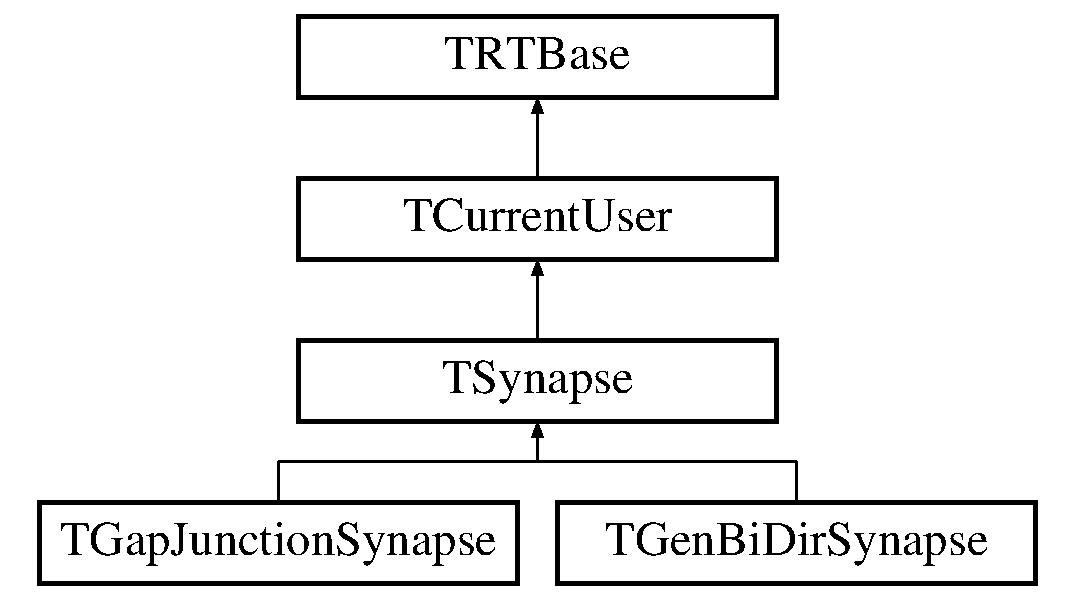
\includegraphics[height=4.000000cm]{class_t_synapse}
\end{center}
\end{figure}
\subsection*{Public Member Functions}
\begin{DoxyCompactItemize}
\item 
\hypertarget{class_t_synapse_afad89e3fd2091900a4e1dc9bc307a694}{virtual \hyperlink{class_t_cell}{T\+Cell} $\ast$const \+\_\+\+\_\+fastcall \hyperlink{class_t_synapse_afad89e3fd2091900a4e1dc9bc307a694}{Pre} ()}\label{class_t_synapse_afad89e3fd2091900a4e1dc9bc307a694}

\begin{DoxyCompactList}\small\item\em Returns a pointer to the presynaptic cell. \end{DoxyCompactList}\item 
\hypertarget{class_t_synapse_a358060ab1845a817039d3611fe886743}{virtual \hyperlink{class_t_cell}{T\+Cell} $\ast$const \+\_\+\+\_\+fastcall \hyperlink{class_t_synapse_a358060ab1845a817039d3611fe886743}{Post} ()}\label{class_t_synapse_a358060ab1845a817039d3611fe886743}

\begin{DoxyCompactList}\small\item\em Returns a pointer to the postsynaptic cell. \end{DoxyCompactList}\item 
\hypertarget{class_t_synapse_a833dfae5d5c3f928fed3329f6cb02267}{virtual \hyperlink{class_t_cell}{T\+Cell} $\ast$const \+\_\+\+\_\+fastcall \hyperlink{class_t_synapse_a833dfae5d5c3f928fed3329f6cb02267}{Pre} () const }\label{class_t_synapse_a833dfae5d5c3f928fed3329f6cb02267}

\begin{DoxyCompactList}\small\item\em const method, Returns a pointer to the presynaptic cell \end{DoxyCompactList}\item 
\hypertarget{class_t_synapse_a6b1e9466948359d9d16bd886c73a171c}{virtual \hyperlink{class_t_cell}{T\+Cell} $\ast$const \+\_\+\+\_\+fastcall \hyperlink{class_t_synapse_a6b1e9466948359d9d16bd886c73a171c}{Post} () const }\label{class_t_synapse_a6b1e9466948359d9d16bd886c73a171c}

\begin{DoxyCompactList}\small\item\em const method, Returns a pointer to the postsynaptic cell \end{DoxyCompactList}\item 
\hypertarget{class_t_synapse_abf23c375476cac34b7cd90f79179b614}{virtual T\+Currents\+Array \+\_\+\+\_\+fastcall \hyperlink{class_t_synapse_abf23c375476cac34b7cd90f79179b614}{Pre\+To\+Post\+Currents} () const }\label{class_t_synapse_abf23c375476cac34b7cd90f79179b614}

\begin{DoxyCompactList}\small\item\em Returns the array of currents affecting the presynaptic cell. \end{DoxyCompactList}\item 
\hypertarget{class_t_synapse_a91a2599e699b1f911dfe90360bcc3bdb}{virtual T\+Currents\+Array \+\_\+\+\_\+fastcall \hyperlink{class_t_synapse_a91a2599e699b1f911dfe90360bcc3bdb}{Post\+To\+Pre\+Currents} () const }\label{class_t_synapse_a91a2599e699b1f911dfe90360bcc3bdb}

\begin{DoxyCompactList}\small\item\em Returns the array of currents affecting the postsynaptic cell. \end{DoxyCompactList}\item 
\hypertarget{class_t_synapse_abaf6c6a071418de34795eabd2cedf242}{bool \hyperlink{class_t_synapse_abaf6c6a071418de34795eabd2cedf242}{Is\+Post\+Synaptic} (\hyperlink{class_t_cell}{T\+Cell} $\ast$const cell)}\label{class_t_synapse_abaf6c6a071418de34795eabd2cedf242}

\begin{DoxyCompactList}\small\item\em Returns true if cell is postsynaptic, false otherwise. \end{DoxyCompactList}\item 
\hypertarget{class_t_synapse_a13c5c3233a1a1cc75f49627bc860d75f}{double \+\_\+\+\_\+fastcall \hyperlink{class_t_synapse_a13c5c3233a1a1cc75f49627bc860d75f}{Update} (\hyperlink{class_t_cell}{T\+Cell} $\ast$const cell, double step)}\label{class_t_synapse_a13c5c3233a1a1cc75f49627bc860d75f}

\begin{DoxyCompactList}\small\item\em Checks if active and if so, calls \hyperlink{class_t_synapse_a3db3cdd754f5f9536717c56e03b61b07}{Do\+Update()} \end{DoxyCompactList}\item 
virtual double \+\_\+\+\_\+fastcall \hyperlink{class_t_synapse_a3db3cdd754f5f9536717c56e03b61b07}{Do\+Update} (\hyperlink{class_t_cell}{T\+Cell} $\ast$const cell, double step)
\begin{DoxyCompactList}\small\item\em Returns the current contribution to cell of this synapse. \end{DoxyCompactList}\item 
\hypertarget{class_t_synapse_abb4e701eeab0c655c77536281c9d7fc8}{virtual bool \+\_\+\+\_\+fastcall \hyperlink{class_t_synapse_abb4e701eeab0c655c77536281c9d7fc8}{Initialize} (bool Reset)}\label{class_t_synapse_abb4e701eeab0c655c77536281c9d7fc8}

\begin{DoxyCompactList}\small\item\em Overrides pure virtual but does nothing. \end{DoxyCompactList}\item 
virtual const \hyperlink{class_t_current}{T\+Current} $\ast$\+\_\+\+\_\+fastcall \hyperlink{class_t_synapse_a40391153a81e8b475c56ba9a9df9fcfc}{Add\+Current} (\hyperlink{class_t_current}{T\+Current} $\ast$c, \hyperlink{class_t_cell}{T\+Cell} $\ast$const to\+Cell)
\begin{DoxyCompactList}\small\item\em Adds a \hyperlink{class_t_current}{T\+Current} $\ast$ to the array of currents in derived class. \end{DoxyCompactList}\item 
virtual void \+\_\+\+\_\+fastcall \hyperlink{class_t_synapse_a21516d391133b6be97c4a63320563f0a}{Remove\+Current} (\hyperlink{class_t_current}{T\+Current} $\ast$c)
\begin{DoxyCompactList}\small\item\em Removes current from class. \end{DoxyCompactList}\item 
\hypertarget{class_t_synapse_a8289fd860026a783dd0cd8ae47c017f5}{\+\_\+\+\_\+fastcall \hyperlink{class_t_synapse_a8289fd860026a783dd0cd8ae47c017f5}{T\+Synapse} ()}\label{class_t_synapse_a8289fd860026a783dd0cd8ae47c017f5}

\begin{DoxyCompactList}\small\item\em Default constructor. \end{DoxyCompactList}\item 
\hypertarget{class_t_synapse_a06372c470201820a66374d982260e612}{\+\_\+\+\_\+fastcall \hyperlink{class_t_synapse_a06372c470201820a66374d982260e612}{T\+Synapse} (const std\+::wstring \&name, \hyperlink{class_t_cell}{T\+Cell} $\ast$const pre, \hyperlink{class_t_cell}{T\+Cell} $\ast$const post)}\label{class_t_synapse_a06372c470201820a66374d982260e612}

\begin{DoxyCompactList}\small\item\em Specialized constructor. \end{DoxyCompactList}\item 
\hypertarget{class_t_synapse_aeb11eb0673e05f9fce5bf470afe373e9}{\+\_\+\+\_\+fastcall \hyperlink{class_t_synapse_aeb11eb0673e05f9fce5bf470afe373e9}{T\+Synapse} (const \hyperlink{class_t_synapse}{T\+Synapse} \&source)}\label{class_t_synapse_aeb11eb0673e05f9fce5bf470afe373e9}

\begin{DoxyCompactList}\small\item\em Copy constructor. \end{DoxyCompactList}\item 
\hypertarget{class_t_synapse_ac7cb27613f7da581c8114991693d544f}{\+\_\+\+\_\+fastcall \hyperlink{class_t_synapse_ac7cb27613f7da581c8114991693d544f}{T\+Synapse} (const \hyperlink{class_t_synapse}{T\+Synapse} \&source, \hyperlink{class_t_cell}{T\+Cell} $\ast$const new\+Pre, \hyperlink{class_t_cell}{T\+Cell} $\ast$const new\+Post)}\label{class_t_synapse_ac7cb27613f7da581c8114991693d544f}

\begin{DoxyCompactList}\small\item\em \char`\"{}\+Duplicate properties with new cells\char`\"{} constructor \end{DoxyCompactList}\item 
\hypertarget{class_t_synapse_a577120f6def957422905ca775f346c0d}{\hyperlink{class_t_synapse}{T\+Synapse} \& \hyperlink{class_t_synapse_a577120f6def957422905ca775f346c0d}{operator=} (const \hyperlink{class_t_synapse}{T\+Synapse} \&source)}\label{class_t_synapse_a577120f6def957422905ca775f346c0d}

\begin{DoxyCompactList}\small\item\em Overloaded assignment operator. \end{DoxyCompactList}\end{DoxyCompactItemize}
\subsection*{Protected Member Functions}
\begin{DoxyCompactItemize}
\item 
\hypertarget{class_t_synapse_a9547ed117272632e891c08c5329a9734}{virtual void const \+\_\+\+\_\+fastcall \hyperlink{class_t_synapse_a9547ed117272632e891c08c5329a9734}{Write\+To\+Stream} (ostream \&stream) const }\label{class_t_synapse_a9547ed117272632e891c08c5329a9734}

\begin{DoxyCompactList}\small\item\em Writes data members to a stream. \end{DoxyCompactList}\item 
\hypertarget{class_t_synapse_a5a7e20bb7ca2beba9c114ff6ae5495f6}{void const \+\_\+\+\_\+fastcall \hyperlink{class_t_synapse_a5a7e20bb7ca2beba9c114ff6ae5495f6}{Read\+From\+Stream} (istream \&stream)}\label{class_t_synapse_a5a7e20bb7ca2beba9c114ff6ae5495f6}

\begin{DoxyCompactList}\small\item\em Reads data members from a stream. \end{DoxyCompactList}\end{DoxyCompactItemize}
\subsection*{Friends}
\begin{DoxyCompactItemize}
\item 
\hypertarget{class_t_synapse_ac98d07dd8f7b70e16ccb9a01abf56b9c}{class \hyperlink{class_t_synapse_ac98d07dd8f7b70e16ccb9a01abf56b9c}{boost\+::serialization\+::access}}\label{class_t_synapse_ac98d07dd8f7b70e16ccb9a01abf56b9c}

\begin{DoxyCompactList}\small\item\em Required for serialization and saving networks to disk. \end{DoxyCompactList}\end{DoxyCompactItemize}


\subsection{Detailed Description}
Base class for current containers that facilitate communication between cells. 

\hyperlink{class_t_synapse}{T\+Synapse} is bidirectional by design and has two arrays of T\+Currents, accessed by \hyperlink{class_t_synapse_abf23c375476cac34b7cd90f79179b614}{Pre\+To\+Post\+Currents()} and \hyperlink{class_t_synapse_a91a2599e699b1f911dfe90360bcc3bdb}{Post\+To\+Pre\+Currents()}. Arrays were chosen rather than single T\+Currents, because it is possible that a single neurotransmitter activates multiple postsynaptic receptors or a synapse might co-\/release transmitters and peptides or some other effector. T\+Synpase owns pointers to the pre-\/ and postsynaptic T\+Cells, accessed through \hyperlink{class_t_synapse_afad89e3fd2091900a4e1dc9bc307a694}{Pre()} and \hyperlink{class_t_synapse_a358060ab1845a817039d3611fe886743}{Post()}.

\begin{DoxyAuthor}{Author}
E. Brady Trexler $<$ebtrexler (at) gothamsci.\+com$>$, 2011 -\/ 2013 
\end{DoxyAuthor}


\subsection{Member Function Documentation}
\hypertarget{class_t_synapse_a40391153a81e8b475c56ba9a9df9fcfc}{\index{T\+Synapse@{T\+Synapse}!Add\+Current@{Add\+Current}}
\index{Add\+Current@{Add\+Current}!T\+Synapse@{T\+Synapse}}
\subsubsection[{Add\+Current}]{\setlength{\rightskip}{0pt plus 5cm}const {\bf T\+Current} $\ast$\+\_\+\+\_\+fastcall T\+Synapse\+::\+Add\+Current (
\begin{DoxyParamCaption}
\item[{{\bf T\+Current} $\ast$}]{c, }
\item[{{\bf T\+Cell} $\ast$const}]{to\+Cell}
\end{DoxyParamCaption}
)\hspace{0.3cm}{\ttfamily [virtual]}}}\label{class_t_synapse_a40391153a81e8b475c56ba9a9df9fcfc}


Adds a \hyperlink{class_t_current}{T\+Current} $\ast$ to the array of currents in derived class. 

Pure virtual --$>$ class is abstract and can only serve as base class derived classes must override and implement


\begin{DoxyParams}{Parameters}
{\em c} & is pointer to \hyperlink{class_t_current}{T\+Current} derived class \\
\hline
{\em to\+Cell} & is a pointer to the cell affected by this current \\
\hline
\end{DoxyParams}


Implements \hyperlink{class_t_current_user_a79db0c0c69ec346073feb748f28717f4}{T\+Current\+User}.

\hypertarget{class_t_synapse_a3db3cdd754f5f9536717c56e03b61b07}{\index{T\+Synapse@{T\+Synapse}!Do\+Update@{Do\+Update}}
\index{Do\+Update@{Do\+Update}!T\+Synapse@{T\+Synapse}}
\subsubsection[{Do\+Update}]{\setlength{\rightskip}{0pt plus 5cm}double \+\_\+\+\_\+fastcall T\+Synapse\+::\+Do\+Update (
\begin{DoxyParamCaption}
\item[{{\bf T\+Cell} $\ast$const}]{cell, }
\item[{double}]{step}
\end{DoxyParamCaption}
)\hspace{0.3cm}{\ttfamily [virtual]}}}\label{class_t_synapse_a3db3cdd754f5f9536717c56e03b61b07}


Returns the current contribution to cell of this synapse. 

This method queries the cell parameter to see if pre-\/ or postsynaptic and calls, in a loop, either -\/\+F\+Pre\+To\+Post\+Currents\mbox{[}i\mbox{]}-\/$>$Update(step, F\+Pre-\/$>$Vm, F\+Post-\/$>$Vm), or -\/\+F\+Post\+To\+Pre\+Currents\mbox{[}i\mbox{]}-\/$>$Update(step, F\+Post-\/$>$Vm, F\+Pre-\/$>$Vm).

It returns the summed current contribution to the cell from this synapse.

{\bfseries  --Derived classes only need override Do\+Update if they do not use the \hyperlink{class_t_current}{T\+Current} members to define current changes. }


\begin{DoxyParams}{Parameters}
{\em cell} & is equal to either \hyperlink{class_t_synapse_afad89e3fd2091900a4e1dc9bc307a694}{Pre()} or \hyperlink{class_t_synapse_a358060ab1845a817039d3611fe886743}{Post()}, and determines direction for current calculation \\
\hline
{\em step} & is in ms, the time since the last call \\
\hline
\end{DoxyParams}
\hypertarget{class_t_synapse_a21516d391133b6be97c4a63320563f0a}{\index{T\+Synapse@{T\+Synapse}!Remove\+Current@{Remove\+Current}}
\index{Remove\+Current@{Remove\+Current}!T\+Synapse@{T\+Synapse}}
\subsubsection[{Remove\+Current}]{\setlength{\rightskip}{0pt plus 5cm}void \+\_\+\+\_\+fastcall T\+Synapse\+::\+Remove\+Current (
\begin{DoxyParamCaption}
\item[{{\bf T\+Current} $\ast$}]{c}
\end{DoxyParamCaption}
)\hspace{0.3cm}{\ttfamily [virtual]}}}\label{class_t_synapse_a21516d391133b6be97c4a63320563f0a}


Removes current from class. 

Pure virtual --$>$ class is abstract and can only serve as base class derived classes must override and implement 

Implements \hyperlink{class_t_current_user_a957583067328b5a251b8d6cacb6ab279}{T\+Current\+User}.



The documentation for this class was generated from the following files\+:\begin{DoxyCompactItemize}
\item 
R\+T\+\_\+\+Synapse.\+h\item 
R\+T\+\_\+\+Synapse.\+cpp\end{DoxyCompactItemize}

\hypertarget{class_t_voltage_clamp___p_i_d___current}{\section{T\+Voltage\+Clamp\+\_\+\+P\+I\+D\+\_\+\+Current Class Reference}
\label{class_t_voltage_clamp___p_i_d___current}\index{T\+Voltage\+Clamp\+\_\+\+P\+I\+D\+\_\+\+Current@{T\+Voltage\+Clamp\+\_\+\+P\+I\+D\+\_\+\+Current}}
}


Implementation of current designed to clamp a cells voltage to a command potential.  


Inheritance diagram for T\+Voltage\+Clamp\+\_\+\+P\+I\+D\+\_\+\+Current\+:\begin{figure}[H]
\begin{center}
\leavevmode
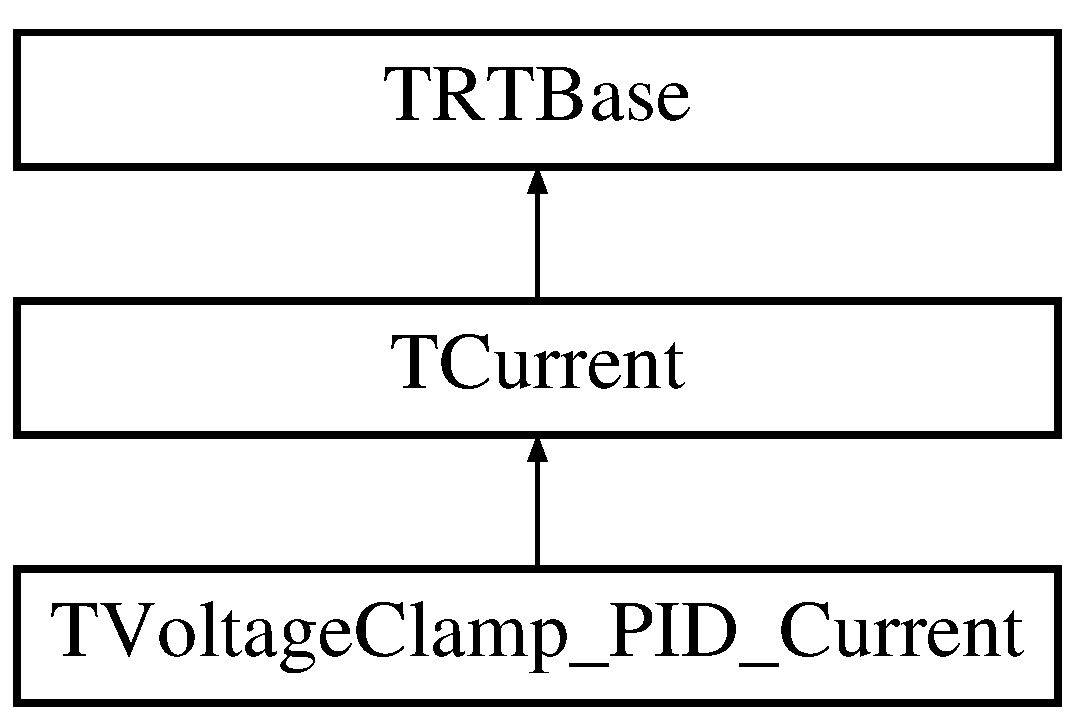
\includegraphics[height=3.000000cm]{class_t_voltage_clamp___p_i_d___current}
\end{center}
\end{figure}
\subsection*{Public Member Functions}
\begin{DoxyCompactItemize}
\item 
bool \+\_\+\+\_\+fastcall \hyperlink{class_t_voltage_clamp___p_i_d___current_a36cfc961ad7b9440318f73fe2ef23e55}{Initialize} (bool Reset)
\begin{DoxyCompactList}\small\item\em Sets Elapsed\+Time to zero. Must be called before first Update. \end{DoxyCompactList}\item 
const std\+::wstring \&\+\_\+\+\_\+fastcall \hyperlink{class_t_voltage_clamp___p_i_d___current_a7be7d4e60396298cad6617d0ab6cfd34}{Class\+Key} () const 
\begin{DoxyCompactList}\small\item\em Returns string used to register class with factory. \end{DoxyCompactList}\item 
const void \+\_\+\+\_\+fastcall \hyperlink{class_t_voltage_clamp___p_i_d___current_aaee131d46d549beb65a598df66a73965}{Get\+Param\+Log\+Header} (std\+::vector$<$ std\+::string $>$ \&params) const 
\begin{DoxyCompactList}\small\item\em Supplies column names for parameter logging. \end{DoxyCompactList}\item 
double \hyperlink{class_t_voltage_clamp___p_i_d___current_a08ef5d1014ae6a1575988185bbcfa0af}{Update\+P\+I\+D} (double step, double error, double position)
\begin{DoxyCompactList}\small\item\em Compute current based on P\+I\+D control. \end{DoxyCompactList}\item 
virtual double \+\_\+\+\_\+fastcall \hyperlink{class_t_voltage_clamp___p_i_d___current_af90e17c7b0f0dbc81040bdc99de4a6e8}{Do\+Update} (double step, double Vkin, double Vdrv, std\+::vector$<$ double $>$ \&params)
\begin{DoxyCompactList}\small\item\em Uses Proportional-\/\+Integral-\/\+Differential method to determine injected current. \end{DoxyCompactList}\item 
\hypertarget{class_t_voltage_clamp___p_i_d___current_ab420c1ac0df81fe6fcb3ff1a0bf395ea}{virtual void \+\_\+\+\_\+fastcall \hyperlink{class_t_voltage_clamp___p_i_d___current_ab420c1ac0df81fe6fcb3ff1a0bf395ea}{Populate\+Edit\+Form} ()}\label{class_t_voltage_clamp___p_i_d___current_ab420c1ac0df81fe6fcb3ff1a0bf395ea}

\begin{DoxyCompactList}\small\item\em Called by G\+U\+I to synchronize edit form with current values of object params. \end{DoxyCompactList}\item 
\hypertarget{class_t_voltage_clamp___p_i_d___current_a7002ebe60a154e87f930b6836f8c95d7}{virtual bool \+\_\+\+\_\+fastcall \hyperlink{class_t_voltage_clamp___p_i_d___current_a7002ebe60a154e87f930b6836f8c95d7}{Validate\+Edit\+Form} ()}\label{class_t_voltage_clamp___p_i_d___current_a7002ebe60a154e87f930b6836f8c95d7}

\begin{DoxyCompactList}\small\item\em Called by G\+U\+I to check if changed values are satisfactory. \end{DoxyCompactList}\item 
\hypertarget{class_t_voltage_clamp___p_i_d___current_a065e523cb852fbca91bd13e5a93bf293}{virtual void $\ast$const \+\_\+\+\_\+fastcall \hyperlink{class_t_voltage_clamp___p_i_d___current_a065e523cb852fbca91bd13e5a93bf293}{Get\+Edit\+Form} ()}\label{class_t_voltage_clamp___p_i_d___current_a065e523cb852fbca91bd13e5a93bf293}

\begin{DoxyCompactList}\small\item\em Returns downcasted T\+Voltage\+Clamp\+\_\+\+P\+I\+D\+\_\+\+Current\+Form$\ast$ that is used to set values for this object. \end{DoxyCompactList}\item 
\hypertarget{class_t_voltage_clamp___p_i_d___current_a9391484c5bb2a33a3d8972bd6a7b4d3c}{\+\_\+\+\_\+fastcall \hyperlink{class_t_voltage_clamp___p_i_d___current_a9391484c5bb2a33a3d8972bd6a7b4d3c}{T\+Voltage\+Clamp\+\_\+\+P\+I\+D\+\_\+\+Current} ()}\label{class_t_voltage_clamp___p_i_d___current_a9391484c5bb2a33a3d8972bd6a7b4d3c}

\begin{DoxyCompactList}\small\item\em default constructor \end{DoxyCompactList}\item 
\hypertarget{class_t_voltage_clamp___p_i_d___current_a8bedf080162f48cebb5614eb3703c913}{\+\_\+\+\_\+fastcall \hyperlink{class_t_voltage_clamp___p_i_d___current_a8bedf080162f48cebb5614eb3703c913}{T\+Voltage\+Clamp\+\_\+\+P\+I\+D\+\_\+\+Current} (\hyperlink{class_t_current_user}{T\+Current\+User} $\ast$owner, const std\+::wstring \&name)}\label{class_t_voltage_clamp___p_i_d___current_a8bedf080162f48cebb5614eb3703c913}

\begin{DoxyCompactList}\small\item\em specialized constructor 2 param \end{DoxyCompactList}\item 
\hypertarget{class_t_voltage_clamp___p_i_d___current_a25b4322894753f9ca41a5fd465ece8e1}{\+\_\+\+\_\+fastcall \hyperlink{class_t_voltage_clamp___p_i_d___current_a25b4322894753f9ca41a5fd465ece8e1}{T\+Voltage\+Clamp\+\_\+\+P\+I\+D\+\_\+\+Current} (const std\+::wstring \&name)}\label{class_t_voltage_clamp___p_i_d___current_a25b4322894753f9ca41a5fd465ece8e1}

\begin{DoxyCompactList}\small\item\em specialized constructor 1 param \end{DoxyCompactList}\item 
\hypertarget{class_t_voltage_clamp___p_i_d___current_a4cac8df237b266af70182298b25ce50e}{\+\_\+\+\_\+fastcall \hyperlink{class_t_voltage_clamp___p_i_d___current_a4cac8df237b266af70182298b25ce50e}{T\+Voltage\+Clamp\+\_\+\+P\+I\+D\+\_\+\+Current} (const \hyperlink{class_t_voltage_clamp___p_i_d___current}{T\+Voltage\+Clamp\+\_\+\+P\+I\+D\+\_\+\+Current} \&source)}\label{class_t_voltage_clamp___p_i_d___current_a4cac8df237b266af70182298b25ce50e}

\begin{DoxyCompactList}\small\item\em copy constructor \end{DoxyCompactList}\item 
\hypertarget{class_t_voltage_clamp___p_i_d___current_a0939de636e6a794ab6e3ed1488011151}{\hyperlink{class_t_voltage_clamp___p_i_d___current}{T\+Voltage\+Clamp\+\_\+\+P\+I\+D\+\_\+\+Current} \& \hyperlink{class_t_voltage_clamp___p_i_d___current_a0939de636e6a794ab6e3ed1488011151}{operator=} (const \hyperlink{class_t_voltage_clamp___p_i_d___current}{T\+Voltage\+Clamp\+\_\+\+P\+I\+D\+\_\+\+Current} \&source)}\label{class_t_voltage_clamp___p_i_d___current_a0939de636e6a794ab6e3ed1488011151}

\begin{DoxyCompactList}\small\item\em overloaded assignment operator \end{DoxyCompactList}\item 
\hypertarget{class_t_voltage_clamp___p_i_d___current_ad58bd13fd1a388cd9091644ec47d907e}{virtual void \+\_\+\+\_\+fastcall \hyperlink{class_t_voltage_clamp___p_i_d___current_ad58bd13fd1a388cd9091644ec47d907e}{Copy\+Params\+From} (const \hyperlink{class_t_current}{T\+Current} $\ast$const source)}\label{class_t_voltage_clamp___p_i_d___current_ad58bd13fd1a388cd9091644ec47d907e}

\begin{DoxyCompactList}\small\item\em overloaded method for duplicating currents without complete assignment \end{DoxyCompactList}\end{DoxyCompactItemize}
\subsection*{Protected Member Functions}
\begin{DoxyCompactItemize}
\item 
\hypertarget{class_t_voltage_clamp___p_i_d___current_aa2a4a186d2c2ebf6c9742f200b81698f}{virtual void const \+\_\+\+\_\+fastcall \hyperlink{class_t_voltage_clamp___p_i_d___current_aa2a4a186d2c2ebf6c9742f200b81698f}{Write\+To\+Stream} (ostream \&stream) const }\label{class_t_voltage_clamp___p_i_d___current_aa2a4a186d2c2ebf6c9742f200b81698f}

\begin{DoxyCompactList}\small\item\em Writes data members to a stream. \end{DoxyCompactList}\item 
\hypertarget{class_t_voltage_clamp___p_i_d___current_a1f31d307ea90b6ffaf869fc7fa9d8886}{virtual void const \+\_\+\+\_\+fastcall \hyperlink{class_t_voltage_clamp___p_i_d___current_a1f31d307ea90b6ffaf869fc7fa9d8886}{Read\+From\+Stream} (istream \&stream)}\label{class_t_voltage_clamp___p_i_d___current_a1f31d307ea90b6ffaf869fc7fa9d8886}

\begin{DoxyCompactList}\small\item\em Reads data members from a stream. \end{DoxyCompactList}\end{DoxyCompactItemize}
\subsection*{Friends}
\begin{DoxyCompactItemize}
\item 
\hypertarget{class_t_voltage_clamp___p_i_d___current_ac98d07dd8f7b70e16ccb9a01abf56b9c}{class {\bfseries boost\+::serialization\+::access}}\label{class_t_voltage_clamp___p_i_d___current_ac98d07dd8f7b70e16ccb9a01abf56b9c}

\end{DoxyCompactItemize}


\subsection{Detailed Description}
Implementation of current designed to clamp a cells voltage to a command potential. 

Uses Proportional-\/\+Integral-\/\+Differential method to determine injected current necessary to hold a cell at a command potential

\begin{DoxyAuthor}{Author}
E. Brady Trexler $<$ebtrexler (at) gothamsci.\+com$>$, 2011 -\/ 2013 
\end{DoxyAuthor}


\subsection{Member Function Documentation}
\hypertarget{class_t_voltage_clamp___p_i_d___current_a7be7d4e60396298cad6617d0ab6cfd34}{\index{T\+Voltage\+Clamp\+\_\+\+P\+I\+D\+\_\+\+Current@{T\+Voltage\+Clamp\+\_\+\+P\+I\+D\+\_\+\+Current}!Class\+Key@{Class\+Key}}
\index{Class\+Key@{Class\+Key}!T\+Voltage\+Clamp\+\_\+\+P\+I\+D\+\_\+\+Current@{T\+Voltage\+Clamp\+\_\+\+P\+I\+D\+\_\+\+Current}}
\subsubsection[{Class\+Key}]{\setlength{\rightskip}{0pt plus 5cm}const std\+::wstring\& \+\_\+\+\_\+fastcall T\+Voltage\+Clamp\+\_\+\+P\+I\+D\+\_\+\+Current\+::\+Class\+Key (
\begin{DoxyParamCaption}
{}
\end{DoxyParamCaption}
) const\hspace{0.3cm}{\ttfamily [inline]}, {\ttfamily [virtual]}}}\label{class_t_voltage_clamp___p_i_d___current_a7be7d4e60396298cad6617d0ab6cfd34}


Returns string used to register class with factory. 

Users of class factories must also tell the class the key they used when registering the class. See factory.\+h 

Implements \hyperlink{class_t_r_t_base_a6083fd510cbcb00faa85e5934fc3c18e}{T\+R\+T\+Base}.

\hypertarget{class_t_voltage_clamp___p_i_d___current_af90e17c7b0f0dbc81040bdc99de4a6e8}{\index{T\+Voltage\+Clamp\+\_\+\+P\+I\+D\+\_\+\+Current@{T\+Voltage\+Clamp\+\_\+\+P\+I\+D\+\_\+\+Current}!Do\+Update@{Do\+Update}}
\index{Do\+Update@{Do\+Update}!T\+Voltage\+Clamp\+\_\+\+P\+I\+D\+\_\+\+Current@{T\+Voltage\+Clamp\+\_\+\+P\+I\+D\+\_\+\+Current}}
\subsubsection[{Do\+Update}]{\setlength{\rightskip}{0pt plus 5cm}virtual double \+\_\+\+\_\+fastcall T\+Voltage\+Clamp\+\_\+\+P\+I\+D\+\_\+\+Current\+::\+Do\+Update (
\begin{DoxyParamCaption}
\item[{double}]{step, }
\item[{double}]{Vkin, }
\item[{double}]{Vdrv, }
\item[{std\+::vector$<$ double $>$ \&}]{params}
\end{DoxyParamCaption}
)\hspace{0.3cm}{\ttfamily [inline]}, {\ttfamily [virtual]}}}\label{class_t_voltage_clamp___p_i_d___current_af90e17c7b0f0dbc81040bdc99de4a6e8}


Uses Proportional-\/\+Integral-\/\+Differential method to determine injected current. 


\begin{DoxyPre}
\begin{DoxyVerb}      Calls UpdatePID with error = Vcommand - Vkin.
        Uses Vkin so a synapse can clamp a cell.  Vdrv is ignored.
\end{DoxyVerb}

\end{DoxyPre}
 

Implements \hyperlink{class_t_current_a36d89025eb424f6905fef945c9ae4fa7}{T\+Current}.

\hypertarget{class_t_voltage_clamp___p_i_d___current_aaee131d46d549beb65a598df66a73965}{\index{T\+Voltage\+Clamp\+\_\+\+P\+I\+D\+\_\+\+Current@{T\+Voltage\+Clamp\+\_\+\+P\+I\+D\+\_\+\+Current}!Get\+Param\+Log\+Header@{Get\+Param\+Log\+Header}}
\index{Get\+Param\+Log\+Header@{Get\+Param\+Log\+Header}!T\+Voltage\+Clamp\+\_\+\+P\+I\+D\+\_\+\+Current@{T\+Voltage\+Clamp\+\_\+\+P\+I\+D\+\_\+\+Current}}
\subsubsection[{Get\+Param\+Log\+Header}]{\setlength{\rightskip}{0pt plus 5cm}const void \+\_\+\+\_\+fastcall T\+Voltage\+Clamp\+\_\+\+P\+I\+D\+\_\+\+Current\+::\+Get\+Param\+Log\+Header (
\begin{DoxyParamCaption}
\item[{std\+::vector$<$ std\+::string $>$ \&}]{params}
\end{DoxyParamCaption}
) const\hspace{0.3cm}{\ttfamily [inline]}, {\ttfamily [virtual]}}}\label{class_t_voltage_clamp___p_i_d___current_aaee131d46d549beb65a598df66a73965}


Supplies column names for parameter logging. 


\begin{DoxyParams}{Parameters}
{\em params} & = vector of parameter names for logging Override in derived classes to add their parameters to the header \\
\hline
\end{DoxyParams}


Implements \hyperlink{class_t_current_ab49cb51723efade5eec00fa78fad7ad8}{T\+Current}.

\hypertarget{class_t_voltage_clamp___p_i_d___current_a36cfc961ad7b9440318f73fe2ef23e55}{\index{T\+Voltage\+Clamp\+\_\+\+P\+I\+D\+\_\+\+Current@{T\+Voltage\+Clamp\+\_\+\+P\+I\+D\+\_\+\+Current}!Initialize@{Initialize}}
\index{Initialize@{Initialize}!T\+Voltage\+Clamp\+\_\+\+P\+I\+D\+\_\+\+Current@{T\+Voltage\+Clamp\+\_\+\+P\+I\+D\+\_\+\+Current}}
\subsubsection[{Initialize}]{\setlength{\rightskip}{0pt plus 5cm}bool \+\_\+\+\_\+fastcall T\+Voltage\+Clamp\+\_\+\+P\+I\+D\+\_\+\+Current\+::\+Initialize (
\begin{DoxyParamCaption}
\item[{bool}]{reset}
\end{DoxyParamCaption}
)\hspace{0.3cm}{\ttfamily [inline]}, {\ttfamily [virtual]}}}\label{class_t_voltage_clamp___p_i_d___current_a36cfc961ad7b9440318f73fe2ef23e55}


Sets Elapsed\+Time to zero. Must be called before first Update. 


\begin{DoxyParams}{Parameters}
{\em reset} & = flag for derived classes \\
\hline
\end{DoxyParams}


Reimplemented from \hyperlink{class_t_current_a00c70d232ae85a9841d8d07e5770b7bd}{T\+Current}.

\hypertarget{class_t_voltage_clamp___p_i_d___current_a08ef5d1014ae6a1575988185bbcfa0af}{\index{T\+Voltage\+Clamp\+\_\+\+P\+I\+D\+\_\+\+Current@{T\+Voltage\+Clamp\+\_\+\+P\+I\+D\+\_\+\+Current}!Update\+P\+I\+D@{Update\+P\+I\+D}}
\index{Update\+P\+I\+D@{Update\+P\+I\+D}!T\+Voltage\+Clamp\+\_\+\+P\+I\+D\+\_\+\+Current@{T\+Voltage\+Clamp\+\_\+\+P\+I\+D\+\_\+\+Current}}
\subsubsection[{Update\+P\+I\+D}]{\setlength{\rightskip}{0pt plus 5cm}double T\+Voltage\+Clamp\+\_\+\+P\+I\+D\+\_\+\+Current\+::\+Update\+P\+I\+D (
\begin{DoxyParamCaption}
\item[{double}]{step, }
\item[{double}]{error, }
\item[{double}]{position}
\end{DoxyParamCaption}
)\hspace{0.3cm}{\ttfamily [inline]}}}\label{class_t_voltage_clamp___p_i_d___current_a08ef5d1014ae6a1575988185bbcfa0af}


Compute current based on P\+I\+D control. 


\begin{DoxyPre}
\begin{DoxyVerb}      computes pTerm + iTerm + (dTerm * step/tau)  ;
\end{DoxyVerb}

\end{DoxyPre}
 

The documentation for this class was generated from the following file\+:\begin{DoxyCompactItemize}
\item 
G\+U\+I\+\_\+\+R\+T\+\_\+\+Edit\+\_\+\+Voltage\+Clamp\+P\+I\+D\+Current.\+cpp\end{DoxyCompactItemize}

\hypertarget{class_t_voltage_clamp___p_i_d___current_form}{\section{T\+Voltage\+Clamp\+\_\+\+P\+I\+D\+\_\+\+Current\+Form Class Reference}
\label{class_t_voltage_clamp___p_i_d___current_form}\index{T\+Voltage\+Clamp\+\_\+\+P\+I\+D\+\_\+\+Current\+Form@{T\+Voltage\+Clamp\+\_\+\+P\+I\+D\+\_\+\+Current\+Form}}
}


G\+U\+I editor for \hyperlink{class_t_voltage_clamp___p_i_d___current}{T\+Voltage\+Clamp\+\_\+\+P\+I\+D\+\_\+\+Current}.  




{\ttfamily \#include $<$G\+U\+I\+\_\+\+R\+T\+\_\+\+Edit\+\_\+\+Voltage\+Clamp\+P\+I\+D\+Current.\+h$>$}

Inheritance diagram for T\+Voltage\+Clamp\+\_\+\+P\+I\+D\+\_\+\+Current\+Form\+:\begin{figure}[H]
\begin{center}
\leavevmode
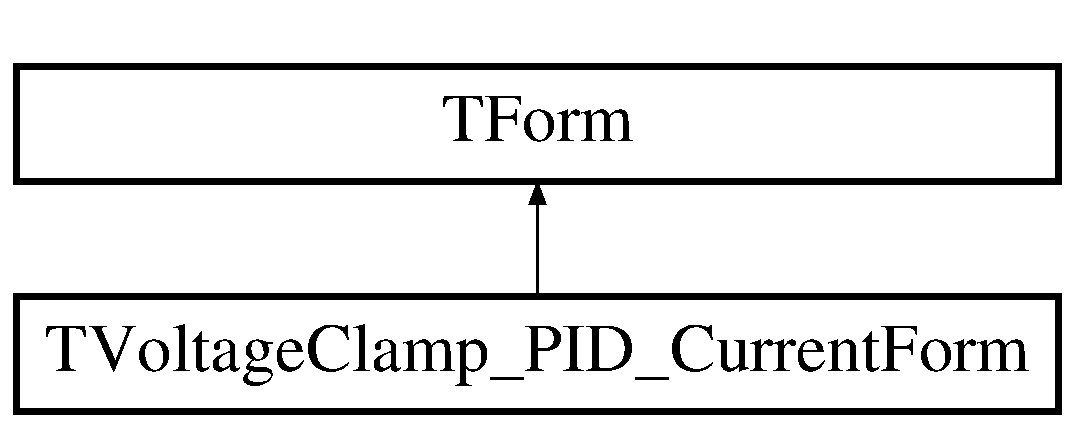
\includegraphics[height=2.000000cm]{class_t_voltage_clamp___p_i_d___current_form}
\end{center}
\end{figure}
\subsection*{Public Member Functions}
\begin{DoxyCompactItemize}
\item 
\hypertarget{class_t_voltage_clamp___p_i_d___current_form_adcbe83e9836425272117042117f440d0}{\+\_\+\+\_\+fastcall {\bfseries T\+Voltage\+Clamp\+\_\+\+P\+I\+D\+\_\+\+Current\+Form} (T\+Component $\ast$Owner)}\label{class_t_voltage_clamp___p_i_d___current_form_adcbe83e9836425272117042117f440d0}

\end{DoxyCompactItemize}
\subsection*{Public Attributes}
\begin{DoxyCompactItemize}
\item 
\hypertarget{class_t_voltage_clamp___p_i_d___current_form_a7d59e831d1887800a51d3e8f40bf0375}{T\+Label $\ast$ {\bfseries Label1}}\label{class_t_voltage_clamp___p_i_d___current_form_a7d59e831d1887800a51d3e8f40bf0375}

\item 
\hypertarget{class_t_voltage_clamp___p_i_d___current_form_a88839e7a3a425aace7ce00c480034436}{T\+Label $\ast$ {\bfseries Label2}}\label{class_t_voltage_clamp___p_i_d___current_form_a88839e7a3a425aace7ce00c480034436}

\item 
\hypertarget{class_t_voltage_clamp___p_i_d___current_form_a8e254b7c1cb8384ce8895bde9eb494a8}{T\+Label $\ast$ {\bfseries Label3}}\label{class_t_voltage_clamp___p_i_d___current_form_a8e254b7c1cb8384ce8895bde9eb494a8}

\item 
\hypertarget{class_t_voltage_clamp___p_i_d___current_form_af6b7d6d2b05cffa0095511724607607f}{T\+Label $\ast$ {\bfseries Label4}}\label{class_t_voltage_clamp___p_i_d___current_form_af6b7d6d2b05cffa0095511724607607f}

\item 
\hypertarget{class_t_voltage_clamp___p_i_d___current_form_a378f77d023775609dae3ec2042327f70}{T\+Edit $\ast$ {\bfseries P\+Gain\+Edit}}\label{class_t_voltage_clamp___p_i_d___current_form_a378f77d023775609dae3ec2042327f70}

\item 
\hypertarget{class_t_voltage_clamp___p_i_d___current_form_ae2bc0a180b4c1a68d612f5bff8026c01}{T\+Edit $\ast$ {\bfseries I\+Gain\+Edit}}\label{class_t_voltage_clamp___p_i_d___current_form_ae2bc0a180b4c1a68d612f5bff8026c01}

\item 
\hypertarget{class_t_voltage_clamp___p_i_d___current_form_a279fb9c27b575b3912a862ce8dd60a1d}{T\+Edit $\ast$ {\bfseries D\+Gain\+Edit}}\label{class_t_voltage_clamp___p_i_d___current_form_a279fb9c27b575b3912a862ce8dd60a1d}

\item 
\hypertarget{class_t_voltage_clamp___p_i_d___current_form_a21cd60b09de7dbd41df36d27743db8dc}{T\+Panel $\ast$ {\bfseries Panel1}}\label{class_t_voltage_clamp___p_i_d___current_form_a21cd60b09de7dbd41df36d27743db8dc}

\item 
\hypertarget{class_t_voltage_clamp___p_i_d___current_form_a06621fff98679081f57b4d743b4ce389}{T\+Edit $\ast$ {\bfseries Tau\+Edit}}\label{class_t_voltage_clamp___p_i_d___current_form_a06621fff98679081f57b4d743b4ce389}

\item 
\hypertarget{class_t_voltage_clamp___p_i_d___current_form_a98e545d99a480323f85376214b5cf211}{T\+Label $\ast$ {\bfseries Label5}}\label{class_t_voltage_clamp___p_i_d___current_form_a98e545d99a480323f85376214b5cf211}

\item 
\hypertarget{class_t_voltage_clamp___p_i_d___current_form_aabc8504486f8d5df90e130dce113dd6f}{T\+Label $\ast$ {\bfseries Label6}}\label{class_t_voltage_clamp___p_i_d___current_form_aabc8504486f8d5df90e130dce113dd6f}

\item 
\hypertarget{class_t_voltage_clamp___p_i_d___current_form_a7200e09c349616fa3a5412bb80df52aa}{T\+Edit $\ast$ {\bfseries V\+Command\+Edit}}\label{class_t_voltage_clamp___p_i_d___current_form_a7200e09c349616fa3a5412bb80df52aa}

\item 
\hypertarget{class_t_voltage_clamp___p_i_d___current_form_a14315f206ca0de91859d54b49be89da0}{T\+Label $\ast$ {\bfseries Label7}}\label{class_t_voltage_clamp___p_i_d___current_form_a14315f206ca0de91859d54b49be89da0}

\item 
\hypertarget{class_t_voltage_clamp___p_i_d___current_form_a0f60b8e081e97c26c915db148d84aba0}{T\+Label $\ast$ {\bfseries Label8}}\label{class_t_voltage_clamp___p_i_d___current_form_a0f60b8e081e97c26c915db148d84aba0}

\item 
\hypertarget{class_t_voltage_clamp___p_i_d___current_form_a8830cb4e81539ee6ff1690301c7096d5}{T\+Edit $\ast$ {\bfseries Imax\+Edit}}\label{class_t_voltage_clamp___p_i_d___current_form_a8830cb4e81539ee6ff1690301c7096d5}

\item 
\hypertarget{class_t_voltage_clamp___p_i_d___current_form_a55f1bfa9ce1f028b6d76eb33a8065576}{T\+Edit $\ast$ {\bfseries Imin\+Edit}}\label{class_t_voltage_clamp___p_i_d___current_form_a55f1bfa9ce1f028b6d76eb33a8065576}

\end{DoxyCompactItemize}


\subsection{Detailed Description}
G\+U\+I editor for \hyperlink{class_t_voltage_clamp___p_i_d___current}{T\+Voltage\+Clamp\+\_\+\+P\+I\+D\+\_\+\+Current}. 

\begin{DoxyAuthor}{Author}
E. Brady Trexler $<$ebtrexler (at) gothamsci.\+com$>$, 2011 -\/ 2013 
\end{DoxyAuthor}


The documentation for this class was generated from the following files\+:\begin{DoxyCompactItemize}
\item 
G\+U\+I\+\_\+\+R\+T\+\_\+\+Edit\+\_\+\+Voltage\+Clamp\+P\+I\+D\+Current.\+h\item 
G\+U\+I\+\_\+\+R\+T\+\_\+\+Edit\+\_\+\+Voltage\+Clamp\+P\+I\+D\+Current.\+cpp\end{DoxyCompactItemize}

\hypertarget{class_t_voltage_clamp_fit_form}{\section{T\+Voltage\+Clamp\+Fit\+Form Class Reference}
\label{class_t_voltage_clamp_fit_form}\index{T\+Voltage\+Clamp\+Fit\+Form@{T\+Voltage\+Clamp\+Fit\+Form}}
}
Inheritance diagram for T\+Voltage\+Clamp\+Fit\+Form\+:\begin{figure}[H]
\begin{center}
\leavevmode
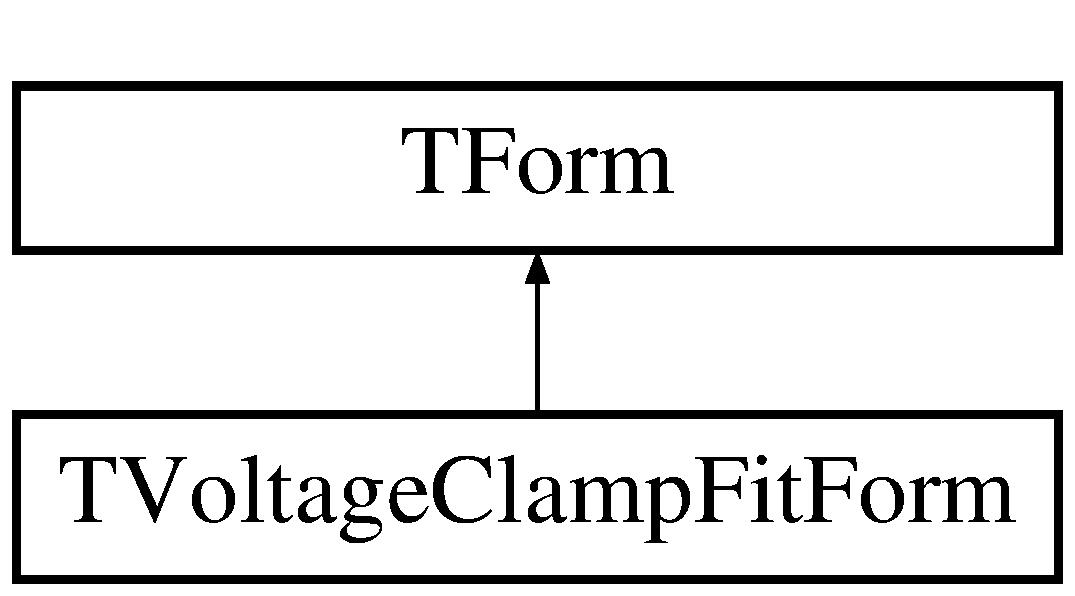
\includegraphics[height=2.000000cm]{class_t_voltage_clamp_fit_form}
\end{center}
\end{figure}
\subsection*{Public Member Functions}
\begin{DoxyCompactItemize}
\item 
\hypertarget{class_t_voltage_clamp_fit_form_ab311a8df380c5f68e2fd660bb6156ef5}{void \+\_\+\+\_\+fastcall {\bfseries Generate\+Button\+Click} (T\+Object $\ast$Sender)}\label{class_t_voltage_clamp_fit_form_ab311a8df380c5f68e2fd660bb6156ef5}

\item 
\hypertarget{class_t_voltage_clamp_fit_form_adfa1a7e8c3e4b8642a0669a315887800}{void \+\_\+\+\_\+fastcall {\bfseries Page\+Control1\+Change} (T\+Object $\ast$Sender)}\label{class_t_voltage_clamp_fit_form_adfa1a7e8c3e4b8642a0669a315887800}

\item 
\hypertarget{class_t_voltage_clamp_fit_form_a9918726cc0ce4232e90dc2ab1f4d2ce4}{void \+\_\+\+\_\+fastcall {\bfseries Page\+Control1\+Changing} (T\+Object $\ast$Sender, bool \&Allow\+Change)}\label{class_t_voltage_clamp_fit_form_a9918726cc0ce4232e90dc2ab1f4d2ce4}

\item 
\hypertarget{class_t_voltage_clamp_fit_form_af093532ff4a4697be6e434fea9dec69c}{void \+\_\+\+\_\+fastcall {\bfseries Save\+Button\+Click} (T\+Object $\ast$Sender)}\label{class_t_voltage_clamp_fit_form_af093532ff4a4697be6e434fea9dec69c}

\item 
\hypertarget{class_t_voltage_clamp_fit_form_a378d81bf328b187863b11b6cad483698}{void \+\_\+\+\_\+fastcall {\bfseries Optimize\+Button\+Click} (T\+Object $\ast$Sender)}\label{class_t_voltage_clamp_fit_form_a378d81bf328b187863b11b6cad483698}

\item 
\hypertarget{class_t_voltage_clamp_fit_form_adab7fb8bb583005aeb5eca825fede65a}{void \+\_\+\+\_\+fastcall {\bfseries Concat\+Epis\+Check\+Box\+Click} (T\+Object $\ast$Sender)}\label{class_t_voltage_clamp_fit_form_adab7fb8bb583005aeb5eca825fede65a}

\item 
\hypertarget{class_t_voltage_clamp_fit_form_a9494d3416cc211e991604ecfc1fda948}{void \+\_\+\+\_\+fastcall {\bfseries Stop\+Button\+Click} (T\+Object $\ast$Sender)}\label{class_t_voltage_clamp_fit_form_a9494d3416cc211e991604ecfc1fda948}

\item 
\hypertarget{class_t_voltage_clamp_fit_form_a4c0da415929e12474485a65b569bac3c}{void \+\_\+\+\_\+fastcall {\bfseries Save\+Params\+Button\+Click} (T\+Object $\ast$Sender)}\label{class_t_voltage_clamp_fit_form_a4c0da415929e12474485a65b569bac3c}

\item 
\hypertarget{class_t_voltage_clamp_fit_form_a4f9bac2baf8d674ee8c159b1c539c4ab}{\+\_\+\+\_\+fastcall {\bfseries T\+Voltage\+Clamp\+Fit\+Form} (T\+Component $\ast$Owner)}\label{class_t_voltage_clamp_fit_form_a4f9bac2baf8d674ee8c159b1c539c4ab}

\end{DoxyCompactItemize}
\subsection*{Public Attributes}
\begin{DoxyCompactItemize}
\item 
\hypertarget{class_t_voltage_clamp_fit_form_a6f13009823c3f938ed80c79d5119c847}{T\+Panel $\ast$ {\bfseries Panel1}}\label{class_t_voltage_clamp_fit_form_a6f13009823c3f938ed80c79d5119c847}

\item 
\hypertarget{class_t_voltage_clamp_fit_form_a1c36e05597f6fbdf993bbffb0adab215}{T\+Panel $\ast$ {\bfseries Panel2}}\label{class_t_voltage_clamp_fit_form_a1c36e05597f6fbdf993bbffb0adab215}

\item 
\hypertarget{class_t_voltage_clamp_fit_form_ab9840c1a8010f2537ef2224db7eb1a18}{T\+Page\+Control $\ast$ {\bfseries Page\+Control1}}\label{class_t_voltage_clamp_fit_form_ab9840c1a8010f2537ef2224db7eb1a18}

\item 
\hypertarget{class_t_voltage_clamp_fit_form_a083e657379c0933838d87f67d7d10a8e}{T\+Tab\+Sheet $\ast$ {\bfseries Tab\+Sheet1}}\label{class_t_voltage_clamp_fit_form_a083e657379c0933838d87f67d7d10a8e}

\item 
\hypertarget{class_t_voltage_clamp_fit_form_a074b769b746e0c854a1cefafbaaeeaed}{T\+Tab\+Sheet $\ast$ {\bfseries Tab\+Sheet2}}\label{class_t_voltage_clamp_fit_form_a074b769b746e0c854a1cefafbaaeeaed}

\item 
\hypertarget{class_t_voltage_clamp_fit_form_aa69292c3cd175decbab84b197cc24fe0}{T\+Tab\+Sheet $\ast$ {\bfseries Tab\+Sheet3}}\label{class_t_voltage_clamp_fit_form_aa69292c3cd175decbab84b197cc24fe0}

\item 
\hypertarget{class_t_voltage_clamp_fit_form_adb7476f58584c03cb86a8f20bbe727fa}{T\+Label $\ast$ {\bfseries Label1}}\label{class_t_voltage_clamp_fit_form_adb7476f58584c03cb86a8f20bbe727fa}

\item 
\hypertarget{class_t_voltage_clamp_fit_form_a270316f2ff6ea397cba772ae696f3321}{T\+Combo\+Box $\ast$ {\bfseries V\+Chan\+Combo\+Box}}\label{class_t_voltage_clamp_fit_form_a270316f2ff6ea397cba772ae696f3321}

\item 
\hypertarget{class_t_voltage_clamp_fit_form_a6a9d70a6b177a7cdd21e29dc1c5bfdd8}{T\+Button $\ast$ {\bfseries Generate\+Button}}\label{class_t_voltage_clamp_fit_form_a6a9d70a6b177a7cdd21e29dc1c5bfdd8}

\item 
\hypertarget{class_t_voltage_clamp_fit_form_a4ac0c2eb4d3b41be2cd0a9e7cf70ca35}{T\+Label $\ast$ {\bfseries Label2}}\label{class_t_voltage_clamp_fit_form_a4ac0c2eb4d3b41be2cd0a9e7cf70ca35}

\item 
\hypertarget{class_t_voltage_clamp_fit_form_a9a30a8fe35d13198ebaa43b6fe676f4e}{T\+Combo\+Box $\ast$ {\bfseries C\+Chan\+Combo\+Box}}\label{class_t_voltage_clamp_fit_form_a9a30a8fe35d13198ebaa43b6fe676f4e}

\item 
\hypertarget{class_t_voltage_clamp_fit_form_af4ff3fff07277f801f650b43e77d7528}{T\+Label $\ast$ {\bfseries Label3}}\label{class_t_voltage_clamp_fit_form_af4ff3fff07277f801f650b43e77d7528}

\item 
\hypertarget{class_t_voltage_clamp_fit_form_a408b4ac4e447fd784058c823a81e5623}{T\+Label $\ast$ {\bfseries Filename\+Label}}\label{class_t_voltage_clamp_fit_form_a408b4ac4e447fd784058c823a81e5623}

\item 
\hypertarget{class_t_voltage_clamp_fit_form_ab8ffa787a780ffd6b36597dd2d13e03b}{T\+Button $\ast$ {\bfseries Save\+Button}}\label{class_t_voltage_clamp_fit_form_ab8ffa787a780ffd6b36597dd2d13e03b}

\item 
\hypertarget{class_t_voltage_clamp_fit_form_a85669ee6d14b2b8a891dbfab2276072c}{T\+Save\+Dialog $\ast$ {\bfseries Save\+Dialog1}}\label{class_t_voltage_clamp_fit_form_a85669ee6d14b2b8a891dbfab2276072c}

\item 
\hypertarget{class_t_voltage_clamp_fit_form_a51c3bc45a6c9b0946e1a7288c3c7e891}{T\+Panel $\ast$ {\bfseries Panel3}}\label{class_t_voltage_clamp_fit_form_a51c3bc45a6c9b0946e1a7288c3c7e891}

\item 
\hypertarget{class_t_voltage_clamp_fit_form_a75ca4059ad7d5b44bc201a3c5c03fff2}{T\+Panel $\ast$ {\bfseries Params\+Panel}}\label{class_t_voltage_clamp_fit_form_a75ca4059ad7d5b44bc201a3c5c03fff2}

\item 
\hypertarget{class_t_voltage_clamp_fit_form_a9fe3d7450962ba2a50a7bf48ee96268c}{T\+P\+L\+O\+T\+Panel $\ast$ {\bfseries Plot\+Panel1}}\label{class_t_voltage_clamp_fit_form_a9fe3d7450962ba2a50a7bf48ee96268c}

\item 
\hypertarget{class_t_voltage_clamp_fit_form_ae7e20aaf54fb34cabc1f577b1c0177fa}{T\+Label $\ast$ {\bfseries Label4}}\label{class_t_voltage_clamp_fit_form_ae7e20aaf54fb34cabc1f577b1c0177fa}

\item 
\hypertarget{class_t_voltage_clamp_fit_form_ac28693d463dc7c2f855b20d77961fc5c}{T\+Check\+Box $\ast$ {\bfseries Concat\+Epis\+Check\+Box}}\label{class_t_voltage_clamp_fit_form_ac28693d463dc7c2f855b20d77961fc5c}

\item 
\hypertarget{class_t_voltage_clamp_fit_form_a95cc49fca2466e35b7e79108c6716265}{T\+Button $\ast$ {\bfseries Optimize\+Button}}\label{class_t_voltage_clamp_fit_form_a95cc49fca2466e35b7e79108c6716265}

\item 
\hypertarget{class_t_voltage_clamp_fit_form_a840987a9c9c2dd8205e287c17a5b2419}{T\+Value\+List\+Editor $\ast$ {\bfseries Value\+List\+Editor1}}\label{class_t_voltage_clamp_fit_form_a840987a9c9c2dd8205e287c17a5b2419}

\item 
\hypertarget{class_t_voltage_clamp_fit_form_ad07ad1e76f8cc63a1f3ded6643a4a523}{T\+Label $\ast$ {\bfseries Label5}}\label{class_t_voltage_clamp_fit_form_ad07ad1e76f8cc63a1f3ded6643a4a523}

\item 
\hypertarget{class_t_voltage_clamp_fit_form_a770e0227ea8bc00e2d20009c9afe7316}{T\+Label $\ast$ {\bfseries fit\+Gen\+Label}}\label{class_t_voltage_clamp_fit_form_a770e0227ea8bc00e2d20009c9afe7316}

\item 
\hypertarget{class_t_voltage_clamp_fit_form_afde04ad7796db00d488ab407fa90a186}{T\+Label $\ast$ {\bfseries Label6}}\label{class_t_voltage_clamp_fit_form_afde04ad7796db00d488ab407fa90a186}

\item 
\hypertarget{class_t_voltage_clamp_fit_form_af030cfac80230d8f0296e9ec5efa6381}{T\+Label $\ast$ {\bfseries Chi\+Sq\+Label}}\label{class_t_voltage_clamp_fit_form_af030cfac80230d8f0296e9ec5efa6381}

\item 
\hypertarget{class_t_voltage_clamp_fit_form_a8f9ba38a997b2cd38cf3b43bc29cc5cc}{T\+Scroll\+Box $\ast$ {\bfseries Scroll\+Box1}}\label{class_t_voltage_clamp_fit_form_a8f9ba38a997b2cd38cf3b43bc29cc5cc}

\item 
\hypertarget{class_t_voltage_clamp_fit_form_a3647bc0279fd881877e4d66aec839faf}{T\+Scroll\+Box $\ast$ {\bfseries Scroll\+Box2}}\label{class_t_voltage_clamp_fit_form_a3647bc0279fd881877e4d66aec839faf}

\item 
\hypertarget{class_t_voltage_clamp_fit_form_ac8a945232f7c2dec4d4f3f41c18e9ec3}{T\+Check\+Box $\ast$ {\bfseries Multi\+Thread\+Check\+Box}}\label{class_t_voltage_clamp_fit_form_ac8a945232f7c2dec4d4f3f41c18e9ec3}

\item 
\hypertarget{class_t_voltage_clamp_fit_form_a515df2eb85f70b5843c900620072613a}{T\+Label $\ast$ {\bfseries Label7}}\label{class_t_voltage_clamp_fit_form_a515df2eb85f70b5843c900620072613a}

\item 
\hypertarget{class_t_voltage_clamp_fit_form_a125a5c559f98754f46ad5bb92e8ae271}{T\+Edit $\ast$ {\bfseries Num\+Threads\+Edit}}\label{class_t_voltage_clamp_fit_form_a125a5c559f98754f46ad5bb92e8ae271}

\item 
\hypertarget{class_t_voltage_clamp_fit_form_aaa0297823e6098041e47ed4253555f21}{T\+Button $\ast$ {\bfseries Stop\+Button}}\label{class_t_voltage_clamp_fit_form_aaa0297823e6098041e47ed4253555f21}

\item 
\hypertarget{class_t_voltage_clamp_fit_form_a90346dff6142d6368b78fe7038a07af0}{T\+Button $\ast$ {\bfseries Save\+Params\+Button}}\label{class_t_voltage_clamp_fit_form_a90346dff6142d6368b78fe7038a07af0}

\item 
\hypertarget{class_t_voltage_clamp_fit_form_a828eed702082447383a34b54a9afcdff}{T\+Save\+Dialog $\ast$ {\bfseries Save\+Dialog2}}\label{class_t_voltage_clamp_fit_form_a828eed702082447383a34b54a9afcdff}

\item 
\hypertarget{class_t_voltage_clamp_fit_form_a67d5e0bf7cbde6f13ccd5984147c3bcf}{double $\ast$ {\bfseries origdata}}\label{class_t_voltage_clamp_fit_form_a67d5e0bf7cbde6f13ccd5984147c3bcf}

\item 
\hypertarget{class_t_voltage_clamp_fit_form_a109b2be4272d5b9aeca636c1b5fbb170}{double $\ast$ {\bfseries genrdata}}\label{class_t_voltage_clamp_fit_form_a109b2be4272d5b9aeca636c1b5fbb170}

\item 
\hypertarget{class_t_voltage_clamp_fit_form_ab029da795d12393380b3db9b5230e006}{\hyperlink{class_t_h_h_current_model}{T\+H\+H\+Current\+Model} {\bfseries H\+H\+Model}}\label{class_t_voltage_clamp_fit_form_ab029da795d12393380b3db9b5230e006}

\end{DoxyCompactItemize}


The documentation for this class was generated from the following files\+:\begin{DoxyCompactItemize}
\item 
G\+U\+I\+\_\+\+Voltage\+Clamp\+Fit\+Form.\+h\item 
G\+U\+I\+\_\+\+Voltage\+Clamp\+Fit\+Form.\+cpp\end{DoxyCompactItemize}

%--- End generated contents ---

% Index
\newpage
\phantomsection
\addcontentsline{toc}{chapter}{Index}
\printindex

\end{document}
